\documentclass[12pt]{article}
\usepackage{amsmath, amsthm, amsfonts, amssymb}
\usepackage{mathtools} % For dcases and \xrightarrow
\usepackage{mathdots}% For the complicated D-module morphism figure
\usepackage[utf8]{inputenc}
\usepackage[all,cmtip]{xy}
\usepackage{xcolor}
\usepackage{graphicx}
\graphicspath{ {./images/} }
\usepackage{url}
\usepackage{csquotes}

% WEIRD: bibtex didn't like the cite key ``humphreys-BGG''
% But was OK when I changed it to ``humphreys.BGG'' for like a minute.
% Then it stopped working again.

%\usepackage{babel}[portuguese]
%\usepackage{geometry}
%\usepackage{cancel}

\usepackage{tikz}
\usepackage{tikz-cd}
%\usepackage{bbm}

\usetikzlibrary{decorations.markings}

\newcommand\Ccancel[2][black]{\renewcommand\CancelColor{\color{#1}}\cancel{#2}}
\newcommand{\vvec}[1]{\vert #1 \rangle}

%%%%%%%%%%%%%%%%%%%%%%%%%%%%%%%%%%%%%%%%%%%%%%%%%%%%%%%%%%%%%%%%%%%%%%%%%%%%%%%%%%%%%%%%
%%%%%%%%%%%%%%%%%%%%%%%%%%%%%%%%%%%%%%%%%%%%%%%%%%%%%%%%%%%%%%%%%%%%%%%%%%%%%%%%%%%%%%%%

\theoremstyle{plain}
\newtheorem{thm}{Theorem}[section]
\newtheorem{lemma}[thm]{Lemma}
\newtheorem{prop}[thm]{Proposition}
\newtheorem{cor}[thm]{Corollary}
\newtheorem{rmrk}[thm]{Remark}
\newtheorem{rem}[thm]{Remark}
\newtheorem{exer}[thm]{Exercise}


\theoremstyle{definition}
\newtheorem{defn}{Definition}[section]
\newtheorem{exmp}{Example}%[section]



\numberwithin{equation}{section}



% LECTURE TAG
\newcommand{\lectag}[2]{\textbf{\color{blue}{#1}. Lecture #2}}

% THE SQUARE BOX AT THE TOP OF THE PAGE
\newcommand{\squarething}[1]{
  \noindent
  \begin{center}
  \framebox{
    \vbox{
      \vspace{4mm}
      \hbox to 5.78in { {\Large \hfill #1  \hfill} }
      \vspace{4mm}
    }
  }
  \end{center}
  \vspace*{4mm}
}

% 1-inch margins, from fullpage.sty by H.Partl, Version 2, Dec. 15, 1988.
\topmargin 0pt
\advance \topmargin by -\headheight
\advance \topmargin by -\headsep
\textheight 8.9in
\oddsidemargin 0pt
\evensidemargin \oddsidemargin
\marginparwidth 0.5in
\textwidth 6.5in

\parindent 0in
\parskip 1.5ex

%%%%%%%%%%%%%%%%%%%%%%%%%%%%%%%%%%%%%%%%%%%%%%%%%%%%%%%%%%%%%%%%%%%%%%%%%%%%%%%%%%%%%%%%
%%%%%%%%%%%%%%%%%%%%%%%%%%%%%%%%%%%%%%%%%%%%%%%%%%%%%%%%%%%%%%%%%%%%%%%%%%%%%%%%%%%%%%%%



\DeclareMathOperator{\Gode}{Gode}
\DeclareMathOperator{\coker}{coker}
\DeclareMathOperator{\spec}{Spec}
\DeclareMathOperator{\sheaves}{Sh}
\DeclareMathOperator{\presheaves}{PreSh}
\DeclareMathOperator{\Ext}{Ext}
\DeclareMathOperator{\Der}{Der}
\DeclareMathOperator{\Stab}{Stab}



\DeclareMathOperator{\shom}{\underline{\Hom}}
\DeclareMathOperator{\Sym}{Sym}

\DeclareMathOperator{\Ad}{Ad}
\DeclareMathOperator{\ad}{ad}
\DeclareMathOperator{\supp}{supp}
\DeclareMathOperator{\Tor}{Tor}
\DeclareMathOperator{\Mor}{Mor}
\DeclareMathOperator*{\colim}{colim}
\DeclareMathOperator{\ch}{Ch}
\DeclareMathOperator{\en}{End}
\DeclareMathOperator{\rk}{Rank}
\DeclareMathOperator{\mult}{mult}
\DeclareMathOperator{\height}{ht}
\DeclareMathOperator{\trans}{{\sf T}}
\DeclareMathOperator{\tr}{Tr}
\DeclareMathOperator{\Hom}{Hom}
\DeclareMathOperator{\sheafHom}{\underline{Hom}}
\DeclareMathOperator{\gr}{gr}
\DeclareMathOperator{\res}{Res}
\DeclareMathOperator{\zhu}{Zhu}
\DeclareMathOperator{\lie}{Lie}
\DeclareMathOperator{\aut}{Aut}
\DeclareMathOperator{\Ind}{Ind}
\DeclareMathOperator{\Id}{Id}
\DeclareMathOperator{\wt}{wt}
\DeclareMathOperator{\img}{im}
\DeclareMathOperator{\Mat}{Mat}
\DeclareMathOperator{\Et}{\acute{E}t}

\DeclareMathOperator{\ev}{ev}
\DeclareMathOperator{\coev}{coev}

\DeclareMathOperator{\BI}{BI}
\DeclareMathOperator{\NI}{NI}
\DeclareMathOperator{\LNI}{LNI}
\DeclareMathOperator{\RNI}{RNI}




\newcommand{\V}{\mathcal{V}}

\newcommand{\what}[1]{\widehat{#1}}
\newcommand{\wtil}[1]{\widetilde{#1}}
\newcommand{\ov}[1]{\overline#1}

\newcommand{\fu}{\mathfrak{u}}
\newcommand{\op}{op}
\newcommand{\M}{\mathcal{M}}
\newcommand{\bbD}{\mathbb{D}}
\newcommand{\im}{im}

\newcommand{\m}{\mathfrak{m}}

\newcommand{\bbA}{\mathbb{A}}


\newcommand{\al}{\alpha}
\newcommand{\la}{\lambda}
\newcommand{\La}{\Lambda}
\newcommand{\Om}{\Omega}
\newcommand{\eps}{\epsilon}
\newcommand{\D}{\Delta}

\newcommand{\C}{\mathbb{C}}
\newcommand{\F}{\mathbb{F}}
\newcommand{\Q}{\mathbb{Q}}
\newcommand{\R}{\mathbb{R}}
\newcommand{\Z}{\mathbb{Z}}
\newcommand{\bbP}{\mathbb{P}}


\newcommand{\frakb}{\mathfrak{b}}
\newcommand{\g}{\mathfrak{g}}
\newcommand{\h}{\mathfrak{h}}
\newcommand{\n}{\mathfrak{n}}
\newcommand{\fb}{\mathfrak{b}}
\newcommand{\gll}{\mathfrak{gl}}
\newcommand{\sll}{\mathfrak{sl}}
\newcommand{\soo}{\mathfrak{so}}
\newcommand{\spp}{\mathfrak{sp}}

\newcommand{\CA}{\mathcal{A}}
\newcommand{\CC}{\mathcal{C}}
\newcommand{\CD}{\mathcal{D}}
\newcommand{\CE}{\mathcal{E}}
\newcommand{\CF}{\mathcal{F}}
\newcommand{\CG}{\mathcal{G}}
\newcommand{\CL}{\mathcal{L}}
\newcommand{\CP}{\mathcal{P}}
\newcommand{\CR}{\mathcal{R}}
\newcommand{\CV}{\mathcal{V}}
\newcommand{\CW}{\mathcal{W}}
\newcommand{\OO}{\mathcal{O}}
\newcommand{\CU}{\mathcal{U}}
\newcommand{\CM}{\mathcal{M}}

\newcommand{\Ass}{\mathbf{Ass}}
\newcommand{\Lie}{\mathbf{Lie}}
\newcommand{\Set}{\mathbf{Set}}
\newcommand{\Vect}{\mathbf{Vec}}



\newcommand{\ma}{\mathfrak{a}}

\newcommand{\Vir}{Vir}

\newcommand{\vac}{\left|0\right>}

\newcommand{\ket}[1]{\left|#1\right>}

\newcommand{\stacksubscript}[2]{\genfrac{}{}{0pt}{}{#1}{#2}}

\newcommand{\tbt}[4]{\left(\begin{array}{cc} #1 & #2 \\ #3 & #4 \\ \end{array}\right)}

%%%%%%%%%%%%%%%%%%%%%%%%%%%%%%%%%%%%%%%%%%%%%%%%%%%%%%%%%%%%%%%%%%%%%%%%%%%%%%%%%%%%%%%%
%%%%%%%%%%%%%%%%%%%%%%%%%%%%%%%%%%%%%%%%%%%%%%%%%%%%%%%%%%%%%%%%%%%%%%%%%%%%%%%%%%%%%%%%
%%%%%%%%%%%%%%%%%%%%%%%%%%%%%%%%%%%%%%%%%%%%%%%%%%%%%%%%%%%%%%%%%%%%%%%%%%%%%%%%%%%%%%%%
%%%%%%%%%%%%%%%%%%%%%%%%%%%%%%%%%%%%%%%%%%%%%%%%%%%%%%%%%%%%%%%%%%%%%%%%%%%%%%%%%%%%%%%%
%%%%%%%%%%%%%%%%%%%%%%%%%%%%%%%%%%%%%%%%%%%%%%%%%%%%%%%%%%%%%%%%%%%%%%%%%%%%%%%%%%%%%%%%
%%%%%%%%%%%%%%%%%%%%%%%%%%%%%%%%%%%%%%%%%%%%%%%%%%%%%%%%%%%%%%%%%%%%%%%%%%%%%%%%%%%%%%%%

\begin{document}

\squarething{Topics in representation theory. IMPA 2024-0}

Jethro van Ekeren \\
%(with figures and computer calculations contributed by Igor Blatt)

%%%%%%%%%%%%%%%%%%%%%%%%%%%%%%%%%%%%%%%%%%%%%%%%%%%%%%%%%%%%%%%%%%%%%%%%%%%%%%%%
%%%%%%%%%%%%%%%%%%%%%%%%%%%%%%%%%%%%%%%%%%%%%%%%%%%%%%%%%%%%%%%%%%%%%%%%%%%%%%%%
%%%%%%%%%%%%%%%%%%%%%%%%%%%%%%%%%%%%%%%%%%%%%%%%%%%%%%%%%%%%%%%%%%%%%%%%%%%%%%%%
%%%%%%%%%%%%%%%%%%%%%%%%%%%%%%%%%%%%%%%%%%%%%%%%%%%%%%%%%%%%%%%%%%%%%%%%%%%%%%%%
%%%%%%%%%%%%%%%%%%%%%%%%%%%%%%%%%%%%%%%%%%%%%%%%%%%%%%%%%%%%%%%%%%%%%%%%%%%%%%%%

%\lectag{2023-01-09}{01}


\tableofcontents



\section{Introduction}

The course will cover some topics in the representation theory of semisimple Lie algebras. For such a Lie algebra, the Weyl character formula expresses the character of a finite dimensional irreducible module in terms of the characters of Verma modules. The irreducible module is finite dimensional exactly when it has a highest weight which is dominant integral. The extension of the character formula to more general highest weights is incredibly subtle, and was the subject of the Kazhdan-Lusztig conjecture, proved in the 1980s by Beilinson-Bernstein and Brylinski-Kashiwara. The proof revolves around the geometry of flag varieties, uses the theory of $D$-modules, and marks the beginning of geometric representation theory. The theorem is too difficult to prove in a one-semester course, but the goal is to learn some of the results and techniques that go into this theory.



% There is material here on a number of topics (especially sheaf theory) which is basically very introductory, but which nevertheless cannot replace a thorough grounding in these topics. It is included, nevertheless, in the hopes of capturing something like what Werner Hertzog calls ``ecstatic truth''. That said, if the reader finds any errors or unclear points, please do let me know.





\section{Review of finite dimensional Lie algebras}

%Vector spaces are almost always over the field $\C$ of complex numbers.

Let's start at the beginning. When we work with vector spaces and algebras, these are generally taken to be defined over the field $\C$ of complex numbers, unless otherwise stated.
\begin{defn}
A Lie algebra is a vector space $\g$ together with a bilinear operation $[,] : \g \times \g \rightarrow \g$ such that
\[
[y, x] = -[x, y]
\]
and
\[
[x, [y, z]] = [[x, y], z] + [y, [x, z]].
\]
\end{defn}
Two basic sources of Lie algebras are as follows. Let $A$ be an associative $\C$-algebra, for example the algebra $\en(V)$ of endomorphisms of a vector space $V$, then $A$ becomes a Lie algebra when equipped with the commutator bracket operation
\[
[a, b] = ab - ba.
\]
For the second source, let $R$ be a commutative $\C$-algebra. A derivation of $R$ is a linear map
\[
D : R \rightarrow R
\]
satisfying
\[
D(ab) = D(a)b + aD(b).
\]
For example $D = d/dx$ is a derivation of the algebra $R = \C[x]$.
%In algebraic geometry commutative algebras are thought of as geometric spaces, called ``affine schemes'', and derivations correspond to vector fields.
The set $\Der(R)$ of derivations of $R$ is a vector space. The composition $D_1 \circ D_2$ of derivations is not a derivation, but the commutator bracket is
\[
[D_1, D_2] = D_1 \circ D_2 - D_2 \circ D_1.
\]
This is another example of a Lie algebra.


Any vector space $V$ with $[x, y] = 0$ for all $x, y \in V$ is a Lie algebra, called an abelian Lie algebra.

\begin{defn}
A Lie algebra $\g$ is called simple if it contains no proper nonzero ideals. A vector subspace $\ma \subset \g$ is a subalgebra if $[\ma, \ma] \subset \ma$ and an ideal if $[\ma, \g] \subset \ma$.
\end{defn}



Examples of finite-dimensional simple Lie algebras:
\begin{itemize}
\item The special linear Lie algebra
\[
\sll_n = \{A \in \Mat_{n} \mid \tr(A) = 0 \},
\]

\item The special orthogonal Lie algebra
\[
\soo_n = \{A \in \Mat_{n} \mid A + A^T = 0\},
\]

\item The symplectic Lie algebra
\[
\spp_{2n} = \{A \in \Mat_{2n} \mid \Omega A + A^T \Omega = 0\}, \quad \text{where} \quad \Omega = \tbt{0}{I_n}{-I_n}{0}.
\]
\end{itemize}
It turns out that all the finite dimensional simple Lie algebras over $\C$, with $5$ exceptions, and contained in these three families. The proof of this fact is the highpoint of a typical first course in Lie algebras. Along the way substantial structure theory of finite dimensional Lie algebras must be developed.

%Remark on $so_{V, B}$ for a general bilinear form $B$.

\begin{defn}
Let $(\cdot, \cdot) : \g \times \g \rightarrow \C$ be a bilinear form. We say that $(\cdot, \cdot)$ is invariant if
\[
([x, y], z) = (x, [y, z])
\]
for all $x, y, z \in \g$.
\end{defn}
For example if $\g = \sll_n$, then
\[
(X, Y) = \tr(XY)
\]
is an invariant bilinear form.  For any finite dimensional Lie algebra $\g$ and $x \in \g$, we write $\ad(x) = [x, -]$. Then the Killing form of $\g$ is by definition
\[
\kappa(X, Y) = \tr_\g \ad(X) \ad(Y).
\]
\begin{exer}
Prove that an invariant bilinear form on a simple Lie algebra must in fact be symmetric.
\end{exer}

\begin{defn}
A semisimple Lie algebra is a direct sum of simple ones
\[
\g = \g_1 \oplus \cdots \oplus \g_s.
\]
\end{defn}
\begin{thm}[Cartan's criterion]
The finite dimensional Lie algebra $\g$ is semisimple if and only if its Killing form is nondegenerate.
\end{thm}
The Killing form thus turns out to be key in determining the structure of simple Lie algebras.

Consider the set of diagonal matrices $\h \subset \g = \sll_n$, and consider an element $h \in \h$ and its bracket
\[
[h, E_{ij}] = (h_i - h_j) E_{ij}.
\]
This is saying that $E_{ij}$ is a simultaneous eigenvector for $\ad(h)$ for all $h \in \h$. The eigenvalues are brought together into an object called a ``weight'', this is a linear function
\[
\alpha_{ij} : \h \rightarrow \C.
\]
The whole of $\sll_n$ actually splits into eigenspaces, indexed by a finite set of such weights
\[
\sll_n = \h \oplus \bigoplus_{i \neq j} \C E_{ij}.
\]
In fact if we write $\varepsilon_i$ for extraction of the ith diagonal entry, then $\alpha_{ij} = \varepsilon_i - \varepsilon_j$.
For example for $n=3$ we have
\[
\begin{tikzpicture}
	\draw[] (0,-2) -- (0,2) (-2,0) -- (2,0);
	\draw[fill] (-0.1,0.1) circle(1.5pt) (0.1,-0.1) circle(1.5pt) (1,0) circle(1.5pt) node[below]{$\alpha_{12}$} (0,1) circle(1.5pt) node[left]{$\alpha_{23}$} (1,1) circle(1.5pt) node[right]{$\alpha_{13} = \alpha_{12} + \alpha_{23}$} (-1,0) circle(1.5pt) (0,-1) circle(1.5pt) (-1,-1) circle(1.5pt);
	\node[anchor = north west] at (-2,2) {$\h^\ast$};
\end{tikzpicture}
\]
% \begin{center}
% \includegraphics[width=80mm]{roots_unsymmetric.png}
% \end{center}

We restrict the Killing form to $(\cdot, \cdot) : \h \times \h \rightarrow \C$, and use it to define
\[
\nu : \h \rightarrow \h^*, \quad \text{and} \quad (\alpha, \beta) = (\nu^{-1}(\alpha), \nu^{-1}(\beta)).
\]
By the way, we use the notation $\left<\la, x\right> = \left<x, \la\right> = \la(x)$ for $x \in \h$ and $\la \in \h^*$.

If we now redraw the roots with angles dictated by the Killing form, then the figure becomes more symmetrical, as follows:
\[
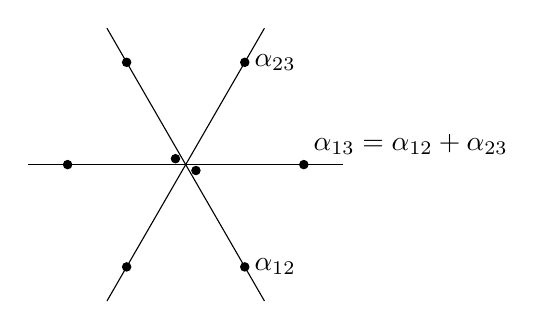
\begin{tikzpicture}
	\foreach \a in {0,120,240} {
	\draw[fill] (\a:1.5cm) circle (1.5pt) (\a+180:1.5cm) circle (1.5pt);
	\draw[] (\a:2cm) -- (\a+180:2cm);
	}
	\draw[fill] (-30:0.15) circle(1.5pt) (150:0.15) circle(1.5pt);
	\node[anchor = south west] at (0:1.5cm) {$\alpha_{13} = \alpha_{12} + \alpha_{23}$};
	\node[right] at (-60:1.5cm) {$\alpha_{12}$};
	\node[right] at (60:1.5cm) {$\alpha_{23}$};
\end{tikzpicture}
\]
% \begin{center}
% \includegraphics[width=80mm]{roots_symmetric.png}
% \end{center}

It turns out that this picture is a pretty good summary of the structure of semisimple Lie algebras in general.
\begin{thm}
Any finite dimensional complex (semi)simple Lie algebra $\g$ has a decomposition
\[
\g = \h \oplus \bigoplus_{\alpha \in \D} \C E_\alpha,
\]
where $\h$ is an abelian subalgebra called the Cartan subalgebra. The dimension of $\h$ is called the rank of $\g$. The weights $\alpha \in \D \subset \h^*$ are called the ``roots'' of $\g$, i.e.,
\[
[h, E_\alpha] = \al(h) E_\alpha \quad \text{for all $h \in \h$}
\]
and
\[
[\g_\alpha, \g_\beta] \subset \g_{\alpha+\beta},
\]
(In fact $[\g_\alpha, \g_\beta] = \g_{\alpha+\beta}$ whenever $\alpha+\beta$ happens to also be a root). The set of roots is invariant under operations
\[
r_\alpha : \beta \mapsto \beta - 2\frac{(\alpha, \beta)}{(\alpha, \alpha)} \alpha.
\]
\end{thm}


{\color{red}GOT TO HERE ON 2024-01-03}

The set
\[
\{\beta + n\alpha \mid n \in \Z\} \cap (\Delta \cup \{0\})
\]
is called the $\alpha$-string through $\beta$. Another key result now.
\begin{thm}
For any pair of roots $\alpha$ and $\beta$ the $\alpha$-string through $\beta$ takes the form
\[
\{\beta-p\alpha, \ldots, \beta, \ldots, \beta+q\alpha\}
\]
and we have
\[
p-q = 2\frac{(\alpha, \beta)}{(\alpha, \alpha)}.
\]
\end{thm}
We split $\Delta$ as $\Delta_+ \cup \Delta_-$ where $\Delta_- = -\Delta_+$. Then we can define simple roots $\{\al_1, \ldots, \al_\ell\}$ as those positive roots that cannot be decomposed into a sum of other positive roots.

For simple roots $\alpha_i$ and $\alpha_j$ we have $\alpha_i - \alpha_i \notin \D$, therefore
\[
a_{ij} = 2 \frac{(\alpha_i, \alpha_j)}{(\alpha_i, \alpha_i)} = -q \leq 0
\]
represents how many times one may add $\alpha_i$ to $\alpha_j$ before leaving $\Delta$. The $\ell \times \ell$-matrix $(a_{ij})$ is called the Cartan matrix of $\g$.

Analysing the Lie algebra $\sll_3$ in this way:
\begin{center}
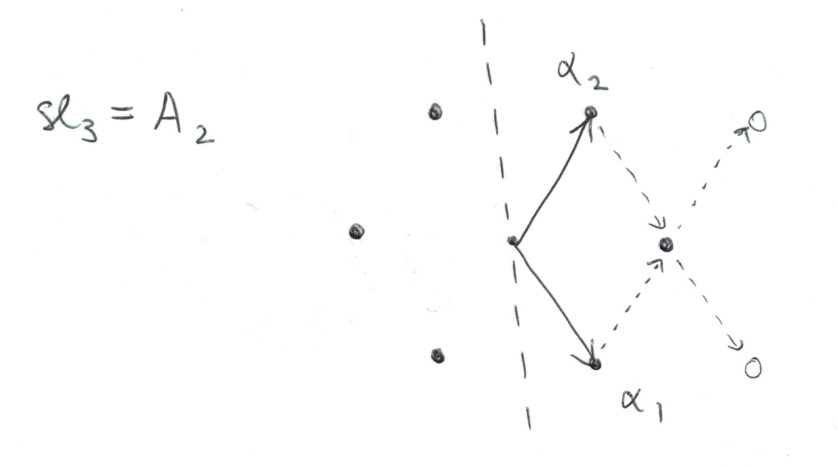
\includegraphics[width=100mm]{A2_Serre.png}
\end{center}
we see that its Cartan matrix must be
\[
\tbt{2}{-1}{-1}{2}.
\]
Similarly, analysing $sp_4$ in this way:
\begin{center}
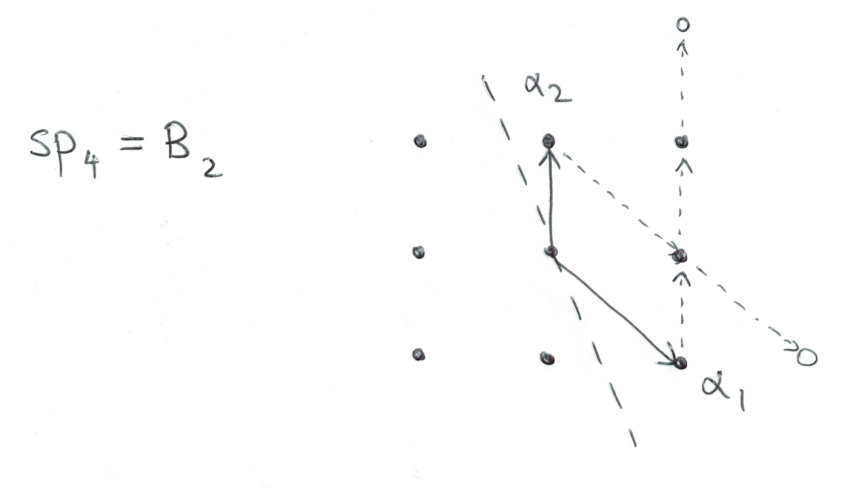
\includegraphics[width=100mm]{B2_Serre.png}
\end{center}
we see (note the importance of getting the order of the roots right) that its Cartan matrix must be
\[
\tbt{2}{-1}{-2}{2}.
\]


% \begin{defn}
% The reflection in the simple root $\al_i$ is the linear transformation $r_i : \h^* \rightarrow \h^*$ defined by
% \[
% r_i(\la) = \la - \left<\la, \al^\vee_i\right> \al_i.
% \]
% One may verify that $(r_i \la, r_i \mu) = (\la, \mu)$ for all $\la, \mu \in \h^*$.
% \end{defn}

\begin{defn}
The Weyl group of $\g(A)$ is the subgroup
\[
W \subset O(\h^*, (\cdot, \cdot))
\]
generated by the root reflections $r_\al$.
\end{defn}

\begin{prop}
In fact $W$ is generated by the reflections $r_1, \ldots, r_\ell$ in simple roots.
\end{prop}



% Writing $E_i = E_{\alpha_i}$, we thus we have the relations
% \[
% \ad(E_i)^{1-a_{ij}} E_j = 0,
% \]
% and similar relations for the $F_i = E_{-\alpha_i}$. Also
% \[
% [E_i, F_j] = 0 \quad \text{for $i \neq j$}.
% \]
% Note also by definition of ``weight'', we have
% \[
% [h, E_i] = \alpha_i(h) E_i, \qquad [h, F_i] = -\alpha_i(h) F_i, \quad \text{for $i=1 \ldots \ell$},
% \]
% and of course
% \[
% [h, h'] = 0 \quad \text{for all $h, h'\in \h$}.
% \]
\begin{lemma}
For each $i = 1, \ldots, \ell$ there exists some nonzero constant $c$ such that
\[
[E_i, F_i] = c \, \nu^{-1}(\alpha_i).
\]
\end{lemma}
It is standard to define
\[
\alpha_i^\vee = \frac{2}{(\alpha_i, \alpha_i)} \nu^{-1}(\alpha_i),
\]
and to normalise $E_i$ and $F_i$ so that
\[
[E_i, F_i] = \alpha_i^\vee.
\]
The reason for this will become clear when we review representation theory.


% \begin{thm}[Serre]
% The generators $E_i$, $F_i$, together with a basis of $\h$, and the relations presented above, define $\g$.
% \end{thm}
% I'll explain this better when we get to Kac-Moody algebras.




\section{Review of modules of finite dimensional simple Lie algebras}

Let $\g$ be a Lie algebra. A $\g$-module (also called a representation of $\g$) is a vector space $V$ and a homomorphism
\[
\rho : \g \rightarrow \en(V)
\]
of Lie algebras, i.e.,
\[
\rho([x, y]) = \rho(x) \rho(y) - \rho(y) \rho(x).
\]
Usually we abuse notation and write $x v$ to stand for $\rho(x)v$.

A vector subspace $W \subset V$ such that $xW \subset W$ for all $x \in \g$ is called a $\g$-submodule. The quotient vector space of a $\g$-module by a $\g$-submodule carries a natural structure of $\g$-module.

PROBLEM 1: Classify all the modules of a Lie algebra $\g$.

Impossible in general, so we restrict to ``nice'', let's say finite dimensional, modules. It's still not really possible in general. But we have
\begin{thm}[Weyl complete reducibility]
If $\g$ is finite dimensional and (semi)simple, then every finite dimensional $\g$-module is isomorphic to a direct sum of irreducible $\g$-modules.
\end{thm}
An irreducible $\g$-module $V$ is one that has no $\g$-submodules other then the trivial ones (namely $0$ and $V$ itself). The proof of this theorem uses Lie algebra cohomology, we will review it soon.

PROBLEM 2: For $\g$ simple, classify and describe the irreducible finite dimensional $\g$-modules.

Now this is possible.

Briefly recall the answer for $\sll_2$. Fix the basis $\{E, H, F\}$ of $\sll_2$ as above, the relations are
\[
[H, E] = 2E, \quad [H, F] = -2F, \quad [E, F] = H.
\]
\begin{thm}
For each nonnegative integer $n \in \Z_+$, there is a unique irreducible module of $\sll_2$ of dimension $n+1$, denoted $V_n$. It looks as follows
\begin{center}
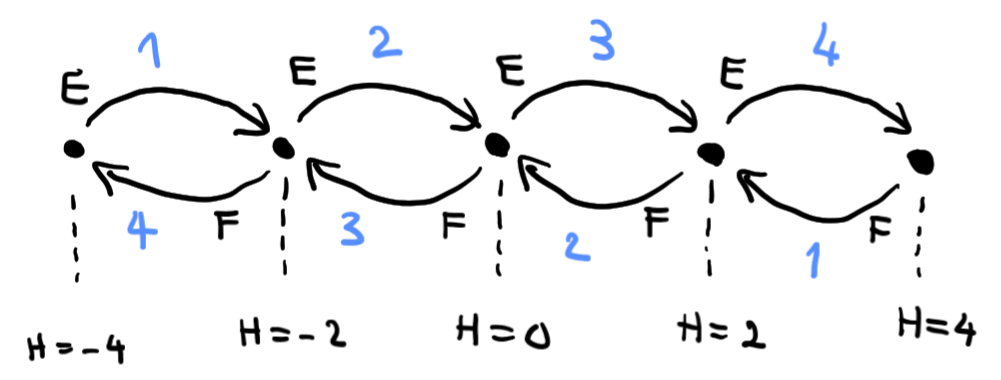
\includegraphics[width=100mm]{sl2_chain_corrected.png}
\end{center}
\end{thm}

{\color{red}GOT TO HERE ON 2024-01-04}






\section{Vermas, irreducibles and category $\OO$}

Let $\g$ be semisimple, and let $M$ be a $\g$-module. A weight space in $M$ is a nonzero subspace $M_\la \subset M$ such that
\[
h v = \la(h) v
\]
for all $h \in \h$ and $v \in M$. Here $\la \in \h^*$ is a weight. If $M$ is a direct sum of weight spaces, we call it a weight module.

The ``support'' of a weight module $M$ is the set
\[
\supp(M) = \{\la \in \h^* \mid M_\la \neq 0\}.
\]


Any finite dimensional irreducible $\g$-module is a weight module. Indeed if we grab a basis $\{H_1, \ldots, H_\ell\}$ of $\h$ then $H_1$ acts in $M$ as some endomorphism, it has an eigenspace which must be stable under $H_2$ since they commute, etc. So there is at least one weight space $M_\la$. But now one can calculate that $E_\al : M_\la \rightarrow M_{\la+\al}$ (which might be zero, but that's no problem). So $M_\la$ is contained in a submodule $M'$ which is a weight module. By irreducibility $M = M'$ is a weight module.




By repeatedly applying elements of $\g_\al$ for $\al \in \D_+$ it is clear that $M$ has one or more ``highest'' weights, in the obvious sense. Precisely, $\La \in \h^*$ is a highest weight of $M$ if $\La \in \supp(M)$ and for all positive roots $\al \in \D_+$ we have $\La + \al \notin \supp(M)$.
\begin{exer}
The highest weight of an irreducible $\g$-module is unique, actually.
\end{exer}


We recall the universal enveloping algebra $U(\g)$ of a Lie algebra $\g$. Let $\{a_1, \ldots, a_N\}$ be a basis of $\g$, then $U(\g)$ is a vector space spanned by words
\[
a_{i_1} a_{i_2} \cdots a_{i_s}
\]
with a natural multiplication given by concatenation, and unit element the empty word $1 = \emptyset$. We regard arbitrary finite strings of elements of $\g$ as elements of $U(\g)$ by imposing distributivity of multiplication over addition. Denote by $i : \g \rightarrow U(\g)$ the linear map sending $x$ to the $1$-letter word $x$.

We also impose a relation that for all $x, y \in \g$ the expression $x y - y x$ in $U(\g)$ is to be identified with $[x, y] \in \g \subset U(\g)$. Formally $U(\g)$ is the quotient of the tensor algebra $T(\g)$ by the $2$-sided ideal generated by $x \otimes y - y \otimes x - [x, y]$ for all $x, y \in \g$.

The algebra $U(\g)$ can be characterised by a ``universal property'', namely for any associative algebra $A$, made into a Lie algebra via $[a, b] = ab-ba$, and homomorphism $\varphi$ of Lie algebras, there exists a unique homomorphism of unital assocative algebras $\widetilde\varphi$ making the following diagram commute
\begin{align*}
\xymatrix{
\g \ar@{->}[dr]^{\varphi} \ar@{->}[rr]^i & & U(\g) \ar@{->}[dl]^{\widetilde\varphi} \\
%
& A & \\
}
\end{align*}

The PBW theorem tells us that $U(\g)$ ``looks like'' a noncommutative version of the polynomial algebra $S(\g)$.
\begin{thm}
The words
\[
a_{i_1} a_{i_2} \cdots a_{i_s}
\]
in which $i_1 \leq i_2 \leq \ldots \leq i_s$ form a basis of $U(\g)$.
\end{thm}

Every $\g$-module becomes a $U(\g)$-module in a unique way such that $i(x) v = xv$.

\begin{defn}
Let $\Lambda \in \h^*$. The Verma module $M(\Lambda)$ of highest weight $\Lambda$ is by definition
\[
M(\La) = U(\g) \otimes_{U(\h \oplus \n_+)} \C_\La,
\]
where $\C_\La = \C v_\Lambda$ is the $1$-dimensional $(\h \oplus \n_+)$-module defined by $\n_+ v_\La = 0$ and $h v_\La = \left<\La, h\right> v_\La$ for all $h \in \h$.
\end{defn}

Recall in general if $A$ is an associative algebra over $\C$ and $M$ and $N$ are right and left $A$-modules, then we have the vector space
\[
M \otimes_A N = \frac{M \otimes_\C N}{(m \cdot a \otimes n = m \otimes a \cdot n)},
\]
with variations for bimodules, etc. By the PBW theorem, as a vector space $M(\La)$ is isomorphic to $U(\n_-)$, and has a basis
\[
f_{i_1} f_{i_2} \cdots f_{i_s} v_\Lambda, \qquad i_1 \leq \ldots \leq i_s,
\]
where $f_1, f_2, \ldots f_N$ is any fixed ordered basis of $\n_-$. By restriction of the action, the $\g$-module $M(\La)$ is also a $U(\n_-)$-module. It is not difficult to see that the association
\begin{align}\label{eq:Un-.basis}
f_{i_1} f_{i_2} \cdots f_{i_s} \mapsto f_{i_1} f_{i_2} \cdots f_{i_s} v_\Lambda,
\end{align}
establishes an isomorphism $U(\n_-) \rightarrow M(\La)$ of $U(\n_-)$-modules.

This isomorphism holds for all weights $\La$, but as $U(\g)$-modules all the different $M(\La)$ are distinct, as we see below, the Verma modules all have different supports, and any two isomorphic weight modules must have the same support.


\begin{defn}
Let $M$ be a $\g$-module, and let $v \in M_\la$ be a vector of weight $\lambda$. Then $v$ is called a singular vector if $\n_+ v = 0$
\end{defn}
Clearly if $\La$ is a highest weight of $M$ then $M_\La$ consists of singular vectors. But there can be other singular vectors in a $\g$-module.

Like the algebra $U(\g)$, the module $M(\La)$ can be characterised by a universal property. A singular vector $v$  in a module $V$ determines a unique morphism
\[
M(\Lambda) \rightarrow V
\]
such that $v_\Lambda \mapsto v$.

Let's introduce some notation. We denote by $Q \subset \h^*$ the $\Z$-linear span of the set $\D$ of roots of $\g$, i.e.,
\[
Q = \{\sum_{i=1}^\ell k_i \al_i \mid k_i \in \Z\}
\]
(We only need to use the simple roots to make linear combinations, because by definition of the notion of simple, all other roots can be written as integer linear combinations of the simple ones.) We denote by
\[
Q_+ = \{\sum_{i=1}^\ell k_i \al_i \mid k_i \in \Z_{\geq 0}\}
\]
the positive cone (equals $\Z_{\geq 0}$-span of $\D_+$). Finally we introduce a partial order on $\h^*$ by saying that
\[
\la \geq \mu \qquad \text{if and only if $\la - \mu \in Q_+$}.
\]



The support of $M(\La)$ is easy to describe. It is convenient to take the $\{f_i\}$ to be a root basis of $\n_-$, namely
\begin{align*}
f_i = E_{-\al_i}
\end{align*}
where $\{\al_1, \ldots, \al_N\}$ is $\D_+$ in some chosen order. The basis vector \eqref{eq:Un-.basis} clearly has weight
\[
\La - \sum_{j=1}^s \al_{i_s}.
\]
Therefore
\[
\supp M(\La) = \La - Q_+.
\]

It is interesting to describe the multiplicities of the weight spaces of $M(\La)$ too.

\begin{center}
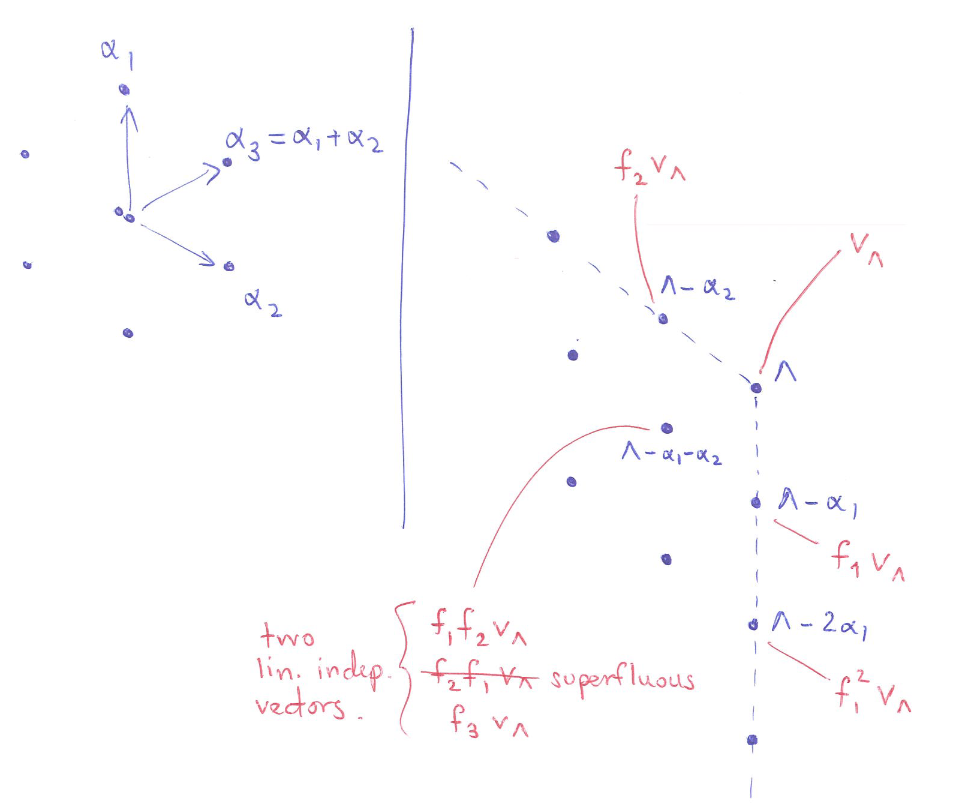
\includegraphics[width=150mm]{Verma-sl3.png}
\end{center}


With a bit of reasoning we see that
\begin{align*}
\dim M(\La)_{\La} &= 1 \\
%
\dim M(\La)_{\La-\al_1} &= \dim M(\La)_{\La-\al_2} = 1 \\
%
\dim M(\La)_{\La-\al_1-\al_2} &= \dim M(\La)_{\La-\al_1-2\al_2} = 2.
\end{align*}
Once we realise that (ultimately because of the PBW theorem) what we are counting here are basis vectors in $\C[f_1, f_2, f_3]$, keeping track of their weights: $\wt(f_1) = -\al_1$, $\wt(f_2) = -\al_2$, $\wt(f_3) = -\al_1-\al_2$, the problem becomes easy.

We write $x_1$ and $x_2$ for the weights $\al_1$ and $\al_2$, so that monomials in $\C[f_1, f_2, f_3]$ become identified with summands in the geometric series expansion of
\[
(1-x_1^{-1})^{-1}(1-x_2^{-1})^{-1}(1-(x_1x_2)^{-1})^{-1}
\]


\begin{defn}
Let $M$ be a weight $\g$-module with finite dimensional weight spaces, then the formal character of $M$ is by definition the sum
\[
\ch_M = \sum_{\lambda \in \h^*} \dim M_\la e^\la.
\]
\end{defn}

In general the character of the Verma module $M(\La)$ is easily seen to be $e^\La / R$ where
\[
R = \prod_{\al \in \D_+} (1 - e^{-\al}).
\]

Example: For the finite dimensional module
\[
L(3\varpi) = M(3\varpi) / J
\]
of $\sll_2$, we have write $x = e^\varpi$
\[
\ch_{M(3\varpi)} = x^3(1 + x^{-2} + x^{-4} + \cdots) = \frac{x^3}{1-x^{-2}}, \qquad \ch_{L(3\varpi)} = x^3 + x + x^{-1} + x^{-3}.
\]



\begin{lemma}
If $I \subseteq M(\La)$ is a submodule then $I = \bigoplus_\la (I \cap M(\La))_\la$.
\end{lemma}

\begin{proof}
This was proved in my Lie algebras course 2022-2 (Lemma 14.5).
\end{proof}

The main use of this lemma to guarantee that the sum of proper submodules of $M(\Lambda)$ is proper (each proper submodule has trivial component in weight $\Lambda$, therefore so too do sums), it follows that there exists a maximal proper submodule $J \subset M(\Lambda)$ (just take the sum of all proper submodules). We denote the quotient (which is irreducible)
\[
L(\La) = M(\La) / J.
\]
We conclude that every finite dimensional irreducible $\g$-module is of this form.

\begin{defn}
The BGG Category $\OO$ is the full subcategory of the category of all $\g$-modules whose objects $M$ satisfy the following conditions
\begin{itemize}
\item $M$ is finitely generated as a $U(\g)$-module,

\item $M$ is a weight module, i.e.,
\[
M = \bigoplus_{\la \in \h^*} M_\la,
\]

\item the action of $\n_+$ on $M$ is locally finite, i.e., for any $v \in M$ we have
\[
\dim U(\n_+) v < \infty.
\]
\end{itemize}
\end{defn}

Some easy consequences of the definition. Proving these is a good exercise for those who have not seen them yet. (See {\cite[Chapter 0]{humbgg}})
\begin{exer}
{\ }
\begin{itemize}
\item The weights of $M$ lie in a finite union of sets of the form $\La - Q_+$.

\item The weight spaces with respect to $\h$ are finite dimensional.
\end{itemize}
\end{exer}


{\color{red}GOT TO HERE ON 2024-01-08}





%There is also a collection of categorical properties satisfied by $\OO$.

Recall the simple roots
\[
\Pi = \{\al_1, \ldots, \al_\ell\},
\]
and for each one the $\sll_2$-triple
\[
E_i, \quad F_i, \quad \al_i^\vee = \frac{2}{(\al_i, \al_i)} \nu^{-1}(\al_i).
\]
Now define
\[
\{\varpi_1, \ldots, \varpi_\ell\} \subset \h^*
\]
to be the basis of $\h^*$ naturally dual to
\[
\Pi^\vee = \{\al_1^\vee, \ldots, \al_\ell^\vee\},
\]
that is $\left< \varpi_i, \al_j^\vee \right> = \delta_{ij}$. These weights are called the \emph{fundamental weights} of $\g$.


\begin{thm}
If $L(\La)$ is finite dimensional, then $\La = \sum_i k_i \varpi_i$ where all $k_i \in \Z_{\geq 0}$.
\end{thm}

By the way, we denote
\[
P_+ = \{ \sum_i k_i \varpi_i \mid \text{ $k_i \in \Z_{\geq 0}$}\}.
\]
Note that $P_+ \not\subset Q_+$ and $Q_+ \not\subset P_+$.


\begin{proof}
Let $v = v_\La$ be a highest weight vector. We consider
\[
v, F_i v, F_i^2 v, \ldots,
\]
this sequence terminates by hypothesis of finite dimensionality, which implies that
\[
\al_i^\vee v = m v \qquad \text{for some integer $m \geq 0$}.
\]
Therefore
\[
\left<\Lambda, \al_i^\vee\right> \in \Z_{\geq 0}.
\]
Conclusion follows.
\end{proof}


\begin{center}
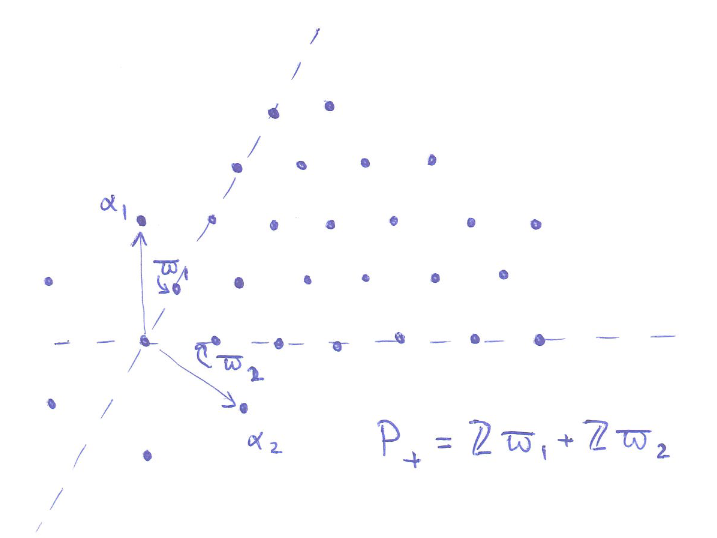
\includegraphics[width=120mm]{P+sl3.png}
\end{center}

In fact the converse is true too.
\begin{thm}\label{thm:P+.implies.fin.dim}
If $\lambda \in P_+$ then $L(\La)$ is finite dimensional.
\end{thm}

There should be some relation between the bases of simple roots and of fundamental weights.
\begin{exer}
Let $\g$ be a finite dimensional simple Lie algebra, so that we know the nondegenerate invariant form $(\cdot, \cdot)$ is unique up to rescaling.
\begin{itemize}
\item Show that the coroots $\al_i^\vee$ are well-defined independent of the choice of $(,)$.

\item Show that the change of basis matrix from $\{\varpi_1, \ldots, \varpi_r\}$ to $\{\al_1, \ldots, \al_r\}$ is the Cartan matrix. More precisely, that
\[
\al_i = \sum_{j=1}^r a_{ji} \varpi_j.
\]
\end{itemize}
\end{exer}

Let us write
\[
Z(\g) = \{z \in U(\g) \mid \text{$zu = uz$ for all $u \in U(\g)$}\}
\]
the centre of $U(\g)$. We shall now write down a very useful element of $Z(\g)$ called the Casimir element.


Let $(,)$ be a nondegenerate invariant bilinear form on $\g$ and let $\{a_i\}$ be a basis of $\g$ and $\{b_i\}$ the corresponding dual basis. That is,
\[
(a_i, b_j) = \delta_{ij}.
\]
The corresponding Casimir element is
\[
\Omega = \sum_{i=1}^{\dim(\g)} a_i b_i \in U(\g).
\]
This element depends on the choice of form $(,)$, but having fixed such a choice it is independent of the choice of basis $\{a_i\}$. Also we recall that if $\g$ is simple then any invariant bilinear form on $\g$ must be a scalar multiple of the Killing form.
\begin{prop}
The operator $\Omega$ commutes with all $x \in \g$ and thus lies in the center of $U(\g)$. In particular if $M$ is an irreducible $\g$-module then $\Omega$ acts as a constant in $M$.
\end{prop}

\begin{proof}
The second part is an immediate consequence of the first part and Schur's lemma. For the first part here is a sketch. Let $x \in \g$ and write $[x, a_i] = \sum_j \alpha_{ij} a_j$ and similarly $[x, b_i] = \sum_j \beta_{ij} b_j$. The key is to use the dual basis relationship to show that $\beta_{ij} = -\al_{ij}$, and obtain a cancelation in
\[
[x, \Om] = \sum([x, a_i]b_i + a_i [x, b_i]).
\]
\end{proof}
Let $M = \bigoplus_{\la} M_\la$ be a weight module. Then since $[h, \Om] = 0$ for all $h \in \h$, we know that $\Om(M_\la) \subset M_{\la}$ for all $\la$. If we further assume that all the weight spaces are finite dimensional (for example if $M \in \OO$), then each weight space has a generalized eigenspace decomposition relative to $\Om$. So we can write
\[
M = \bigoplus_{\gamma \in \C} M^{(\gamma)}
\]
where
\[
M^{(\gamma)} = \{m \in M \mid \text{there exists $N \in \Z_{\geq 0}$ such that $(\Om-\gamma)^N m = 0$}\}.
\]
Notice that each of these vector space summands is actually a $\g$-module. So in many arguments in category $\OO$, it is possible to assume without loss of generality that $M = M^{(\gamma)}$ for some single $\gamma$.



Let us compute the Casimir in some modules of $\sll_2$. We take the symmetric bilinear form
\[
(E, F) = 1, \quad (H, H) = 2,
\]
which is invariant, and
\[
\Omega = EF + FE + \frac{1}{2} H^2 = 2FE + \frac{1}{2}H(H+2).
\]
If we evaluate this operator on the highest weight vector $v$ of weight $\lambda$ (so $Ev = 0$ and $Hv = \lambda v$) then
\[
\Omega = \frac{1}{2}\lambda(\lambda+2).
\]
A little more formally, we have $\al^\vee = H$ and $\varpi \in \h^*$ characterised by $\varpi(H) = 1$. Then the highest weight $\la = a \varpi$ for some $a \in \C$, and $H v = a v$, so
\[
\Omega = \frac{1}{2}a(a+2).
\]
Our normalisation of the bilinear form has it that $(\al, \al) = 2$, but $\varpi = \al / 2$, so $(\varpi, \varpi) = 1/2$. Thus really
\[
\Omega = (\la, \la + 2\varpi).
\]
In fact this is a special case of a general fact.
\begin{defn}
The Weyl vector of $\g$ is the following sum
\[
\rho = \frac{1}{2} \sum_{\al \in \D_+} \al.
\]
\end{defn}
\begin{prop}
Let $\g$ be semisimple, let $M$ be a weight $\g$-module and let $v \in M_\la$ be a singular vector of weight $\la \in \h^*$. Then
\[
\Om v = (\la, \la+2\rho) v.
\]
\end{prop}

\begin{proof}
We choose a basis $\{h_1, \ldots, h_\ell\}$ of $\h$ and complete it to a basis of $\g$ by adding in the root vectors $E_{\al}$ and $F_\al$ as $\al$ runs over $\D_+$. Because of the structure of the Killing form, the dual vector to $E_\al$ is some multiple of $F_\al$ and vice versa. Let $\{h_1', \ldots, h_\ell'\}$ be the basis of $\h$ dual to $\{h_1, \ldots, h_\ell\}$.

Now we compute
\begin{align*}
\Omega v &= \sum_i h_i h'_i v + \sum_{\al \in \D_+} ( E_\al F_\al + F_\al E_\al ) v \\
%
&= \sum_i \la(h_i) \la(h'_i) v + \sum_{\al \in \D_+} ( [E_\al, F_\al] + 2 F_\al E_\al ) v \\
%
&= (\la, \la) v + \sum_{\al \in \D_+} \al^\vee v \\
%
&= (\la, \la) v + \sum_{\al \in \D_+} \la(\al^\vee) v
\end{align*}
{\color{red}(I lost a factor of $2/(\al, \al)$ somehow!)} This simplifies to
\[
(\la, \la+2\rho) v
\]
as required.
\end{proof}

\begin{cor}
Let $M$ be a weight $\g$-module, $v \in M_\la$ a singular vector, and $w \in U(\g) v$ another singular vector, this one of weight $\mu$. Then
\[
(\mu, \mu+2\rho) = (\la, \la+2\rho).
\]
\end{cor}

\begin{proof}
We know that $\Om v = (\la, \la+2\rho) v$, and now because $\Om u = u \Om$ for all $u \in U(\g)$ we see that $\Om w = (\la, \la+2\rho) w$. But we also know that $\Om w = (\mu, \mu+2\rho) w$, so we are done.
\end{proof}
Another convenient way to phrase the relation above is
\[
|\mu+\rho|^2 = |\la+\rho|^2.
\]


\begin{prop}
\[
\rho = \sum_{i=1}^\ell \varpi_i.
\]
\end{prop}

\begin{proof}
Exercise.
\end{proof}

Example of $M = M(2\varpi)$ for $\sll_2$. There are two singular vectors: the highest weight vector in weight $\la = 2\varpi$, and another one in weight $\mu = -4\varpi$.
\begin{center}
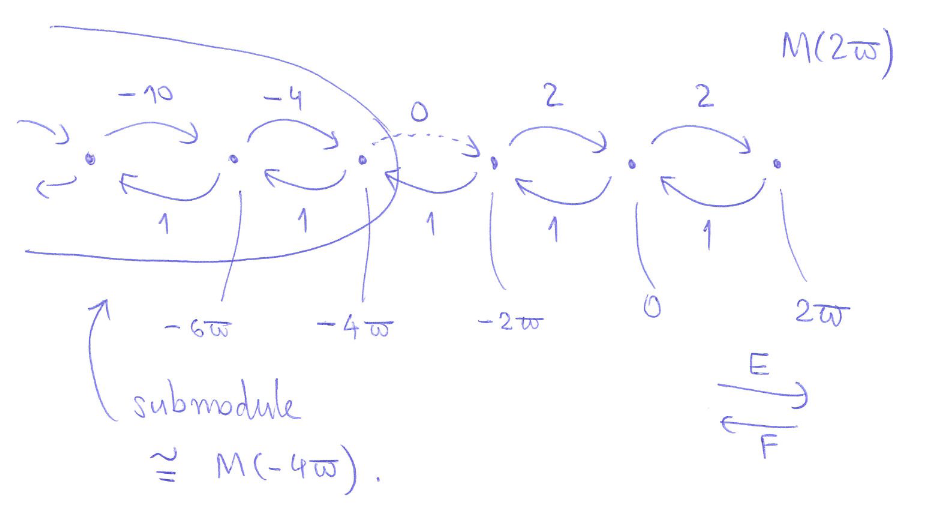
\includegraphics[width=130mm]{M2-M-4-inclusion.png}
\end{center}
We have $\rho = \varpi$, and $\la+\rho = 3\varpi$ and $\mu+\rho = -3\varpi$ clearly have the same norm, as expected.


The notion of abelian category is very important. Roughly speaking an abelian category is a category $\CC$ in which morphisms $f, g : X \rightarrow Y$ can be added and subtracted, and in which there are the notions of kernel $\ker(f) \in \CC$ and cokernel $\coker(f) \in \CC$ of a morphism $f : X \rightarrow Y$, characterised by universal properties. Notions of injective and surjective morphism (more formally known as ``monomorphism'' and ``epimorphism'', respectively) can then be recovered, as well as the ``image'' of a morphism, etc.
\begin{defn}
An object $P$ in an abelian category is \emph{projective} if for every surjection $\pi$ and morphism $\varphi$ as in this diagram, there exists $\widetilde \varphi$ completing it (i.e., such that $\pi \circ \wtil{\varphi} = \varphi$)
\begin{align*}
\xymatrix{
 & M \ar@{->>}[d]^{\pi} \\
%
P \ar@{->}[r]_{\varphi} \ar@{->}[ur]^{\wtil{\varphi}} & N \\
}
\end{align*}
\end{defn}

Recall that a basic example of an abelian category is the category of all left modules over a fixed ring $A$. For example the category of all $\g$-modules is equivalent to the category of all left $U(\g)$-modules, which is an abelian category.

In such categories, we can consider the free modules $A^{\oplus n}$, and it is easy to show that these are projective. In fact in such categories the projective modules are precisely the modules that occur as a summand of some free $A$-module.

Now it is a basic proposition that $\OO$ is also an abelian category. But it is a proper subcategory of $U(\g)$-mod and in particular it is clear that it does not contain any of the free $U(\g)$-modules. So a priori it is not clear whether $\OO$ contains any projective objects. But in fact it does.
\begin{prop}
Suppose $\La \in P_+$, then the Verma module $M(\La)$ is projective.
\end{prop}

\begin{proof}
We consider this situation
\begin{align*}
\xymatrix{
 & M \ar@{->>}[d]^{\pi} \\
%
M(\La) \ar@{->}[r]_{\varphi} \ar@{->}[ur]^{\wtil{\varphi}} & N \\
}
\end{align*}
Let $\ov v = \varphi(v_\La) \in N$ and choose a preimage $v \in M$ of $\ov v$, which we can because $\pi$ is surjective.

Since $\Om v_\La = (\La, \La+2\rho) v_\La$ we also have $\Om \ov v = (\La, \La+2\rho) \ov v$. Let us write $g = (\La, \La+2\rho)$, so that $\ov v \in N^{(g)}$. There is also a decomposition $M = \bigoplus_{\gamma \in \C} M^{(\gamma)}$ and it is possible to choose $v \in M^{(g)}$.

Now consider $U(\n_+)v \subset M$. This vector subspace is finite dimensional and has a weight space decomposition, so it has at least one maximal weight $\La'$, in other words there is some nonzero $w \in M_{\La'}$ such that $w = uv$ for some $u \in U(\n_+)$ and $\n_+ w = 0$. Clearly $w \in M^{(g)}$, and it follows that
\[
(\La, \La+2\rho) = (\La', \La'+2\rho).
\]

We now suppose $\La' \neq \La$ with the aim of deriving a contradiction. In this case we have $\La' = \La + \beta$ for some $\beta \in Q_+$. We have
\begin{align*}
(\La', \La'+2\rho) - (\La, \La+2\rho) &= |\La'+\rho|^2 - |\La+\rho|^2 \\
%
&= |\La+\rho+\beta|^2 - |\La+\rho|^2 \\
%
&= 2(\La+\rho, \beta) + |\beta|^2.
\end{align*}
Since $\rho = \sum_i \varpi_i$ and $\La \in P_+$ we have also $\La+\rho \in P_+$, and since $\beta \in Q_+$ we have $(\La+\rho, \beta) \geq 0$. On the other hand $|\beta|^2 \geq 0$ with equality only for $\beta = 0$, so we have our contradiction.

Knowing now that $\La' = \La$, we see that $w=v$ up to a scalar, and therefore $\n_+v = 0$ or rather, $v$ is a singular vector. By the universal property of $M(\La)$ there exists a morphism $\wtil{\varphi} : M(\La) \rightarrow M$ sending $v_\La \mapsto v$. This is map we wanted to construct. So $M(\La)$ is projective.
\end{proof}




% \begin{defn}
% A projective cover of $M \in \OO$ is $P \in \OO$ projective together with an essential surjection $\pi : P \rightarrow M$ (the surjection $\pi$ is said to be essential if there exists no nontrivial submodule $P_0 \subset P$ such that the restriction $\pi|_{P_0}$ be also surjective).
% \end{defn}
%
% Exercise: Show that all projective covers of an object $M$ (if any exist) are isomorphic to each other.


%Consider $\g = \sll_2$. In a typical block of $\OO$ there are exactly $5$ indecomposable modules.





We recall that for any $\g$-module $M$, the dual vector space $M^*$ acquires a natural $\g$-module structure, via
\[
[x \varphi](m) = -\varphi(x m).
\]
One problem with (or feature of) the category $\OO$ is that it is not closed under this operation. Firstly the dual of a vector space of infinite but countable dimension, is of uncountable dimension.


It is possible to ``correct'' the definition of the dual. Let
\[
\tau : \g \rightarrow \g
\]
be an anti-automorphism of order $2$, satisfying $\tau(h) = h$ for all $h \in \h$ and $\tau(\g_\al) = \g_{-\al}$ for all roots $\al$. For $\sll_n$ for example, taking $\tau(X) = X^T$ would work. It is possible to construct such $\tau$ in general.
\begin{defn}
Let $M = \bigoplus_{\la \in \h^*} M_\la$ be a $\g$-module in category $\OO$. The \emph{contragredient} module $M^\vee$ is by definition $M^\vee = \bigoplus_{\la \in \h^*} M_\la^*$ with the action of $\g$ defined by
\[
[x \varphi](m) = \varphi(\tau(x) m).
\]
\end{defn}
Since $\tau$ acts as the identity on $\h$, we have
\[
(M^\vee)_\la = (M_\la)^* \subset M^\vee.
\]
We could, if we had wished to, define $M^\vee$ with $\tau = -1$, but then we would have
\[
(M^\vee)_\la = (M_{-\la})^* \subset M^\vee,
\]
and modules in $\OO$ would not in general go to other modules in $\OO$. Notice also that the characters of $M$ and $M^\vee$ are equal.

\begin{prop}
If $M \in \OO$ then also $M^\vee \in \OO$.
\end{prop}

{\color{red}Is $\tau$ unique??}

Let's do a couple of examples of contragredient modules for $\g = \sll_2$. Here are the Verma modules $M(2\varpi)$ and $M(-4\varpi)$ (there clearly exists an embedding $M(-4\varpi) \subset M(2\varpi)$).

\begin{center}
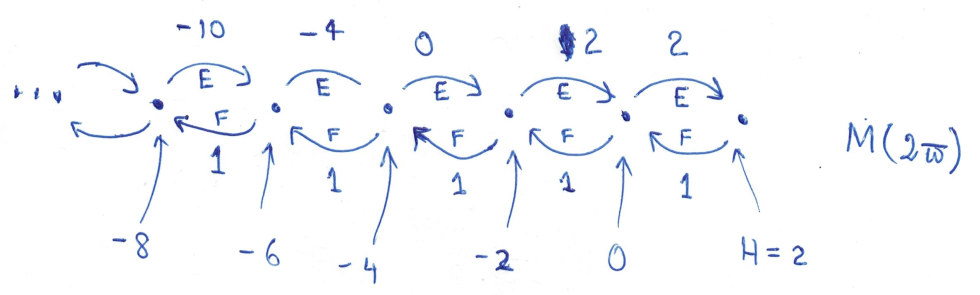
\includegraphics[width=100mm]{M-2.png}
\end{center}

\begin{center}
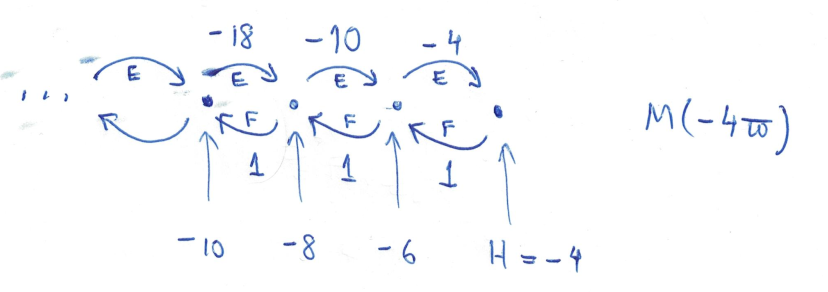
\includegraphics[width=90mm]{M-minus-4.png}
\end{center}



Upon taking the contragredient, we know that the set of weight spaces, and their multiplicities, remain the same. But now the coefficients of $F$ become the coefficients of $E$ and vice versa.


\begin{center}
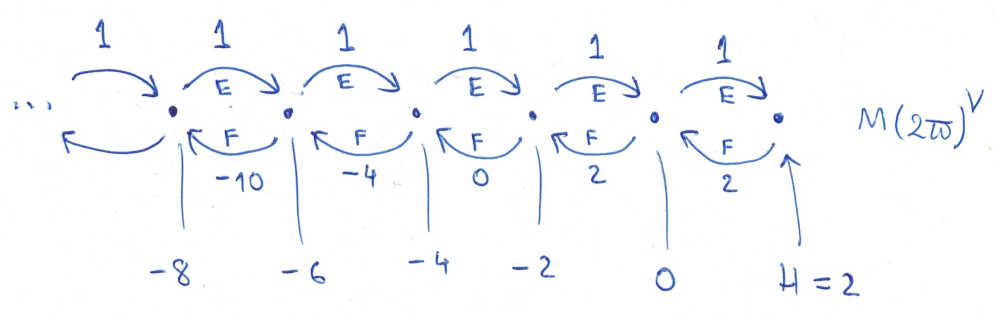
\includegraphics[width=100mm]{M-2-dual.png}
\end{center}

\begin{center}
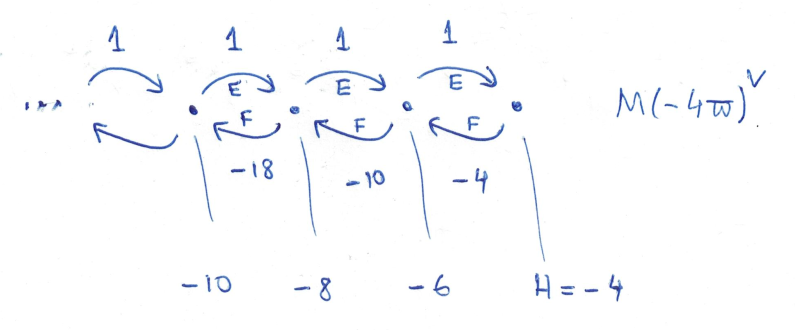
\includegraphics[width=100mm]{M-minus-4-dual.png}
\end{center}


If you think about it, you will see that $M(-4\varpi)^\vee \cong M(-4\varpi)$. If we write $v_{-4}, v_{-6}, \ldots$ for the basis vectors of $M(-4\varpi)$ and $\phi_{-4}, \phi_{-6}, \ldots$ for the corresponding dual vectors which form a basis of $M(-4\varpi)^\vee$, then we can build an isomorphism inductively by $v_{-4} \mapsto \phi_{-4}$, then $v_{-6} \mapsto (-4) \phi_{-6}$, then $v_{-8} \mapsto (-40) \phi_{-8}$, and so on.

Notice that this argument does not work for $M(2\varpi)^\vee$ because we would have to map one of the basis vectors to $0$, so we would not obtain an isomorphism. And indeed $M(2\varpi)^\vee \not\cong M(2\varpi)$. For instance $M(2\varpi)^\vee$ contains a copy of $L(2\varpi)$ while $M(2\varpi)$ does not.

Yet $M(2\varpi)^\vee$ is still an object of $\OO$. Indeed the module is generated by $\phi_2$ and $\phi_{-4}$ (actually we only need $\phi_{-4}$), it is a weight module (by construction), and the action of $\n_+$ is locally finite.


{\color{red}Got up to here on 2024-01-10}

Let $\CC$ be a $\C$-linear abelian category (I just mean every space $\Hom(X, Y)$ is a vector space over $\C$, and $\CC$ is an abelian category) and $X \in \CC$ an object. We can consider the functor
\[
\Hom(X, -) : \CC \rightarrow \Vect.
\]
It is clear that this is a functor, as a morphism $f : A \rightarrow B$ induces a morphism $\Hom(X, A) \rightarrow \Hom(X, B)$ by composition $\phi \mapsto f \circ \phi$. Suppose $A \rightarrow B$ then it is basically clear that
\[
\Hom(X, A) \subset \Hom(X, B),
\]
as two different morphisms to $A$ continue to be different after putting $A$ inside $B$. In other words $\Hom(X, -)$ sends injections to injections.

The same is not true for surjections! Indeed
\begin{defn}
The object $P$ is said to be projective if the functor $\Hom(P, -)$ sends surjections to surjections. That is, if for every $\varphi \in \Hom(P, C)$ there exists $\wtil\varphi \in \Hom(P, B)$ such that $p \circ \wtil{\varphi} = \varphi$
\begin{align*}
\xymatrix{
B \ar@{->>}[r]^{p} & C \\
%
 & P \ar@{->}[u]_{\varphi} \ar@{-->}[ul]^{\wtil{\varphi}} \\
}
\end{align*}
\end{defn}
This is usually phrased in the language of short exact sequences (SES). A SES is $A \subset B$ and $C \cong B/A$, or equivalently $p : B \twoheadrightarrow C$ with $A = \ker(p)$, and in any case is written as
\begin{align}\label{eq:SES}
0 \rightarrow A \rightarrow B \rightarrow C \rightarrow 0.
\end{align}
In general $\Hom(X, -)$ is \emph{left exact}, i.e.,
\[
0 \rightarrow \Hom(X, A) \rightarrow \Hom(X, B) \rightarrow \Hom(X, C).
\]
A functor $F$ which preserves surjections is called \emph{right exact}
\[
F(A) \rightarrow F(B) \rightarrow F(C) \rightarrow 0,
\]
and a functor (like $\Hom(P, -)$ for $P$ projective) which preserves both, is called \emph{exact}
\[
0 \rightarrow \Hom(P, A) \rightarrow \Hom(P, B) \rightarrow \Hom(P, C) \rightarrow 0.
\]

Another name for a short exact sequence \eqref{eq:SES} is an \emph{extension}. The trivial extension where $B = A \oplus C$ with the obvious inclusion $i$ and projection $p$, is also known as a \emph{split} SES. Determining when SES are split and not split is a very important topic.

For now we can make one easy observation
\begin{lemma}
If $P$ is projective then any SES of the form
\begin{align*}%\label{eq:SES}
0 \rightarrow A \rightarrow B \rightarrow P \rightarrow 0
\end{align*}
is split.
\end{lemma}

\begin{proof}
We apply the first definition of projective, to the situation \begin{align*}
\xymatrix{
B \ar@{->>}[r]^{p} & P \\
%
 & P \ar@{->}[u]_{1} \ar@{-->}[ul]^{\wtil{\varphi}} \\
}
\end{align*}
The image of $\wtil{\varphi}$ in $B$ must be an object complementary to the image of $A$ in $B$. So $B$ is the direct sum of these images.
\end{proof}

% \begin{rem}
% Apparently there is a subtlety here, about whether or not we assume existence of arbitrary products and coproducts. Maybe this is just a Reimundice.
% \end{rem}


Like usual in category theory, notions come in pairs. The dual notion to projective object is injective object, whose definition is obtained by reversing all arrows.
\begin{defn}
An object $I$ is said to be \emph{injective} if for all $i$ and $\varphi$ there exists $\wtil{\varphi}$ as in the diagram
\begin{align*}
\xymatrix{
A \ar@{^{(}->}[r]^{i} \ar@{->}[d]_{\varphi} & B \ar@{-->}[dl]^{\wtil{\varphi}} \\
%
I  \\
}
\end{align*}
\end{defn}
We now also get the dual lemma
\begin{lemma}
If $I$ is injective then any SES of the form
\begin{align*}%\label{eq:SES}
0 \rightarrow I \rightarrow B \rightarrow C \rightarrow 0
\end{align*}
is split.
\end{lemma}


\begin{lemma}
The irreducible objects of $\OO$ are precisely the $\g$-modules $L(\La)$ for $\La \in \h^*$.
\end{lemma}

\begin{proof}
Any object in $\OO$ has at least one highest weight vector. So let $v_\La$ be one such for our simple object. This induces a nonzero morphism $M(\La) \rightarrow M$, which image is a submodule of $M$ and so must be all of $M$. So we have a surjection $M(\La) \rightarrow M$. The kernel is contained in the maximal graded submodule, and if it were not equal, the image of the maximal graded submodule would be a nontrivial submodule of $M$. So we are done.
\end{proof}

%PROBLEM: Find a general formula for the character of $L(\La)$.

{\color{red}We noticed that the proof of projectivity of $M(\La)$ works not only for $\La \in P_+$, but far more generally, even for a dense set of weights $\La$. I drew a picture illustrating this. TO DO: Write out this discussion, and include it and the picture here.}


\begin{defn}
Let $\gamma \in \C$, we define the ``very weak block''\footnote{Jethro's terminology, no one really calls it by this name.} $\OO^{(\gamma)}$ to be the subcategory of $\OO$ consisting of objects $M$ which satisfy $M = M^{(\gamma)}$.
\end{defn}
As we have seen, any object of $\OO$ decomposes into a direct sum of objects in distinct very weak blocks. But on the other hand, each very weak block contains an uncountable number of non-isomorphic objects (in particular instance all the Verma modules $M(\la)$ for $|\la+\rho|^2-|\rho|^2 = \gamma$).

We have seen in the discussion above that we can do better. For example let us consider $M(\la)$ and $M(\mu)$ in the same very weak block, i.e.,
\[
|\la+\rho|^2 = |\mu+\rho|^2.
\]
If we do not also have $\la-\mu \notin Q$, then $\la \notin \supp M(\mu)$ and $\mu \notin \supp M(\la)$, so there is no way for there to exist a morphism $M(\la) \rightarrow M(\mu)$, and vice versa. The two modules ``cannot interact'' in some sense.



To capture this idea in a clean way we make the following definition.
\begin{defn}
A \emph{composition series} of $M \in \OO$ is a sequence of submodules
\[
M = M_0 \supset M_1 \supset \ldots \supset M_n \supset M_{n+1} = 0,
\]
such that each quotient $L_i = M_i / M_{i+1}$ is irreducible.
\end{defn}



\begin{prop}\label{prop:weak-block-condition}
Each object of $\OO$ has a composition series.
\end{prop}


{\color{blue}I skipped the proof in class, but here it is in full.}


\begin{proof}
Let $M = \bigoplus_{\gamma \in \C} M^{(\gamma)}$ be the decomposition into generalised eigenspaces of $\Omega$. Without loss of generality we may assume $M = M^{(\gamma)}$, i.e., $\Omega - \gamma$ is locally nilpotent on $M$.

The idea is to start with the series
\[
M = M_0 \supset M_1 = 0.
\]
If $M$ is irreducible, we are done. If not then there is a submodule $S$ which we may insert into the series:
\[
M = M_0 \supset S \supset M_2 = 0.
\]
Then we continue looking for submodules of $S$ and submodules of $M_0$ containing $S$, etc. The question is why this process should terminate in a finite number of steps.

We shall simultaneously keep track of the characters of the quotient modules. For each weight $\mu$ we have
\[
\dim(M_0)_\mu \geq \dim(M_1)_\mu \geq \ldots \geq \dim(M_n)_\mu \geq 0,
\]
Since $\dim(M_0)_\mu$ is finite, clearly there comes a time after which new quotients have zero $\mu$-weight space.

We know that on a highest weight vector of weight $\lambda$ the operator $\Omega$ acts as $(\la, \la + 2\rho)$. But since the Killing form is positive definite\footnote{Only if we work over the reals! So I am cheating a bit here, we are also using that the roots are defined over the reals.}, the set of possible highest weights of subquotients is finite.

Note that we are not claiming that any given submodule $M_i$ is generated by a singular vector. The following could happen

\begin{center}
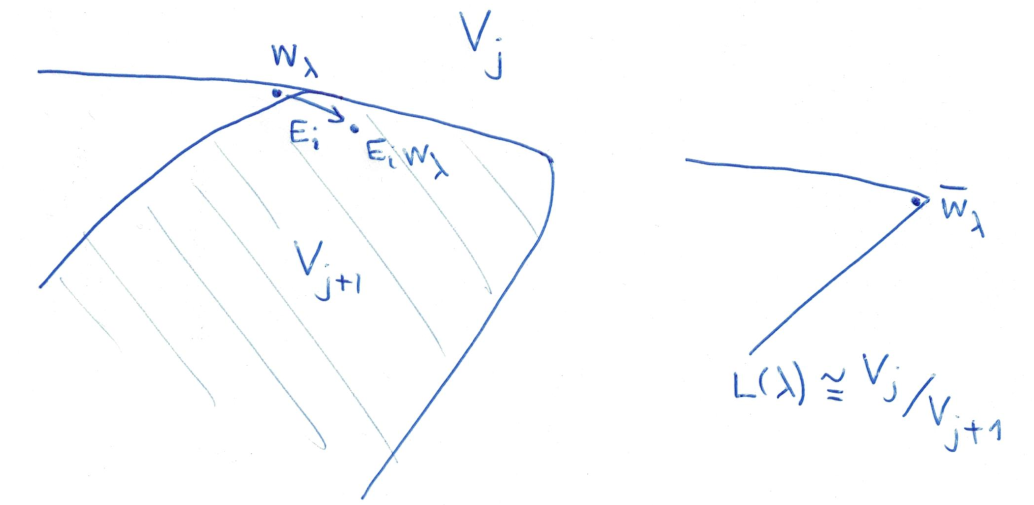
\includegraphics[width=110mm]{subsing.png}
\end{center}

Nevertheless we know that $\Omega$ descends to the same scalar on the quotient $M_i / M_{i+1}$.
\end{proof}

\begin{prop}%\label{prop:weak-block-condition} {\ }
If $L(\la)$ is a composition factor of $M(\Lambda)$, then $\La \geq \la$ and
\[
|\la + \rho|^2 = |\La+\rho|^2.
\]
\end{prop}

\begin{proof}
The first condition on $\la$ is clear since $\supp M(\La) = \La - Q_+$, and the second follows from the fact that $\Omega$ acts in $M(\La)$ by the scalar $(\La, \La+2\rho)$, and thus acts by this constant in all subquotients.
\end{proof}

Now we can define (weak) blocks.
\begin{defn}
The ``weak block'' $\OO^{[\la]}$ consists of all objects of $\OO$ whose composition factors are of the form $L(\la_i)$ where
\begin{itemize}
\item $\la_i - \la \in Q$,

\item $|\la_i+\rho|^2 = |\la+\rho|^2$.
\end{itemize}
\end{defn}
In other words we have specified a certain equivalence class on weights $\la \in \h^*$, and defined weak blocks to consist of objects with composition factors $L(\la_i)$ where all $\la_i$ come from a single equivalence class. By the theory we have developed so far we can prove:
\begin{prop}
Each object of $\OO$ decomposes into a direct sum of objects, which all lie in distinct weak blocks.
\end{prop}

For the majority of weights $\la \in \h^*$ the intersection of the sets
\[
\{\mu \in \h^* \mid |\mu+\rho|^2 = |\la+\rho|^2 \}
\]
and
\[
\la + Q
\]
is $\{\la\}$. In such a case we have $L(\la) = M(\la)$ and the only objects in $\OO^{[\la]}$ are direct sums of copies of $M(\la)$. The other extreme, in some sense, is the case in which $\la \in P$. This is the case we shall generally focus on.

\begin{rem}
Of course there is one case in which the weak block $\OO^{[\la]}$ is small, even though the weight is integral, namely $\la = -\rho$. Then for all weights $\mu = -\rho+\al \in -\rho+Q$ we have
\[
|\mu+\rho|^2 = |\al|^2 > 0,
\]
while $|-\rho+\rho|^2 = 0$. In particular $M(-\rho)$ is irreducible. %In fact $M(\La)$ is irreducible for any ``sufficiently negative'' weight $\La$. You might enjoy trying to find conditions that guarantee this.
\end{rem}

%If $\La$ is irrational then $M(\La) = L(\La)$ already, and if $\La$ is rational then in a certain sense the problem can be reduced to the case that $\La$ is integral. So we restrict attention to $\La \in P$.

If $\la \in \h^*$ and $w \in W$ then we can consider the following operation:
\[
w \circ \la = w(\la+\rho) - \rho.
\]
Since $w : \h^* \rightarrow \h^*$ is an orthogonal transformation (i.e., $(w(\la), w(\mu)) = (\la, \mu)$) we see that
\[
|w\circ \la + \rho|^2 = |\la+\rho|^2.
\]
If we further assume $\la \in P$ then $w\circ\la - \la \in Q$, so all the weights
\[
\{L(w \circ \la) \mid w \in W\}
\]
lie in the same weak block $\OO^{[\la]}$.



In fact a stronger relation on composition factors can be proved.
\begin{prop}\label{prop:block-condition}
Let $L(\la)$ be a composition factor of $M(\Lambda)$. Then $\La \geq \la$ and
\[
\la = w(\La+\rho) - \rho
\]
for some $w \in W$.
\end{prop}
The proof of this is not difficult, but it will come somewhat later in the course. It uses the \emph{Harish-Chandra isomorphism} This result motivates the following definition.
\begin{defn}
The ``block'' $\OO^{\la}$ consists of all objects of $\OO$ whose composition factors are of the form $L(\la_i)$ where
\begin{itemize}
\item $\la_i - \la \in Q$,

\item $\la_i = w \circ \la$ for some $w\in W$.
\end{itemize}
\end{defn}
It is then possible to prove:
\begin{prop}
Each object of $\OO$ decomposes into a direct sum of objects, which all lie in distinct blocks.
\end{prop}




\section{The Weyl complete reducibility theorem}

Let $\g$ be a Lie algebra and $A$, $C$ two $\g$-modules. An extension of $A$ by $C$ is a short exact sequence of $\g$-modules
\[
0 \rightarrow A \rightarrow B \rightarrow C \rightarrow 0.
\]
More precisely, two such SES are considered isomorphic if there exists an isomorphism $B \rightarrow B'$ such that
\begin{align*}
\xymatrix{
0 \ar@{->}[r] & A \ar@{->}[r] \ar@{->}[d]_{1} & B \ar@{->}[r] \ar@{->}[d] & C \ar@{->}[r] \ar@{->}[d]^{1} & 0 \\
%
0 \ar@{->}[r] & A \ar@{->}[r] & B' \ar@{->}[r] & C \ar@{->}[r] & 0 \\
}
\end{align*}
commutes. One can actually define the category of extensions of $A$ by $C$, with morphisms being any morphism $B \rightarrow B'$ making the diagram above commute. Then the $5$-lemma implies that any such morphism is actually an isomorphism. In fancy language this means the category of extensions of $A$ by $C$ is a \emph{groupoid}.

Any SES of vector spaces is split. Let us take an extension as above, and randomly choose a splitting at the level of vector spaces, i.e.,
\begin{align*}
\xymatrix{
0 \ar@{->}[r] & A \ar@{->}[r]^{i} & B \ar@{->}[r]^{p} & C \ar@{->}[r] \ar@/^1.0pc/@[][l]^{s} & 0 \\
}
\end{align*}
where $p \circ s = 1_C$. Consider the following construction: For $x \in \g$ and $c \in C$ the element
\[
x s(c) - s(x c)
\]
lies in $\ker(p) = \img(i)$. Thus we have a $\C$-linear map
\begin{align*}
\g &\rightarrow \Hom(C, A) \\
%
x &\mapsto (c \mapsto [x, s] c).
\end{align*}
Write $M = \Hom(C, A)$ and $\xi_B$ for the linear map.

You might observe that $M = \Hom(C, A)$ is naturally a left $\g$-module, which prompts the question of whether $\xi_B$ is a morphism of $\g$-modules. In general it is not. What is the $\g$-module structure of $M$? Well $\Hom(C, A) \cong C^* \otimes A$ and we know that $C^*$ is a $\g$-module via
\[
[x f](c) = -f(xc),
\]
and $C^* \otimes A$ is a $\g$-module via
\[
x(f \otimes a) = (xf) \otimes a + f \otimes (xa),
\]
so that
\[
[x\xi](c) = x\xi(c) - \xi(xc).
\]
There is a functor from $\g$-modules to vector spaces of \emph{$\g$-invariants}, denoted $M \mapsto M^\g$, and it is clear that
\begin{align*}
\Hom_\g(C, A) = \Hom(C, A)^{\g}.
\end{align*}

Below we shall introduce the Chevalley-Eilenberg complex of $\g$, for now we just consider:
\begin{align*}
M \rightarrow \Hom(\g, M) \rightarrow \Hom(\wedge^2\g, M) \rightarrow \cdots
\end{align*}
(these are spaces of $\C$-linear morphisms, not $\g$-linear morphisms). Let us write $\delta$ for the differentials, the first for example is (if $m \in M$)
\[
\delta(m) : x \mapsto x m,
\]
and the second is (if $f \in \Hom(\g, M)$)
\[
\delta(f) : x \wedge y \mapsto x f(y) - y f(x) - f([x, y]).
\]





Anyway, our extension $B$ has given us an element $\xi_B$ of $\Hom(\g, M)$. Actually, has it really? We had to choose a splitting $s$ to define $\xi_B$. Suppose we chose a different splitting $s'$, then we would obtain the different map
\[
\xi_B' : x \mapsto (c \mapsto [x, s']c).
\]
Let us consider the difference between $\xi_B$ and $\xi_B'$. It will act as
\[
x \mapsto (c \mapsto [x, s - s']c).
\]
Observe that $p(s-s')c = c-c=0$, so $(s-s')c \in \ker(p) = \img(i) = A$. Thus the difference $s-s'$ has given us a linear morphism $C \rightarrow A$, i.e., an element $\eta \in \Hom(C, A) = M$. Now the map
\[
x \mapsto (c \mapsto [x, \eta]c)
\]
is $\delta(\eta)$! So the element $\xi_B$ is not well-defined as an element of $\Hom(\g, M)$, but it is well-defined modulo $\img(\delta)$.

One also checks that $\xi_B \in \ker(\delta)$. So there is a well-defined class
\[
[\xi_B] \in H^1(\g, M) = \frac{\ker(\delta)}{\img(\delta)}.
\]
It is a theorem that $B \mapsto [\xi_B]$ is an isomorphism from the isomorphism classes of extensions to $H^1(\g, M)$. How is this proved? Well, $[\xi_B] = 0$ just means that there is some $\eta \in M$ such that $\xi_B = \delta(\eta)$, i.e.,
\[
(x \mapsto (c \mapsto [x, s]c)) = (x \mapsto (c \mapsto [x, \eta]c))
\]
or rather
\[
[x, s]c = [x, \eta]c
\]
for all $x \in \g$ and all $c \in C$. But now we can use $\eta$ to ''correct'' $s$, setting $\wtil{s} = s - \eta$. Since $\eta(c) \in A$ we have $p \circ \wtil{s} = 1$ as required, but now
\[
x \wtil{s}(c) = \wtil{s}(xc),
\]
so $\wtil{s}$ is a morphism of $\g$-modules. Therefore vanishing of $[\xi_B]$ has been used to exhibit a splitting of the extension $B$, as required.


\begin{defn}
A Lie algebra $\g$ is said to be semisimple if it contains no nonzero solvable ideal.
\end{defn}
\begin{thm}[Cartan's criterion]
A Lie algebra $\g$ is semisimple if and only if its Killing form is nondegenerate.
\end{thm}
This version (the semisimple version) of Cartan's criterion is equivalent to another version (the solvable version)
\begin{thm}\label{thm:CC.sol}
Let $\g \subset \en(M)$ be a Lie subalgebra. Then $(\g, [\g, \g])_M = 0$ if and only if $\g$ is solvable.
\end{thm}
One direction of this follows easily from Lie's theorem. The other direction is very tricky.



\begin{prop}[Whitehead]
Let $\g$ be a semisimple Lie algebra and $M$ a finite dimensional $\g$-module. Then $H^1(\g, M) = 0$.
\end{prop}


\begin{proof}
We will have to use Cartan's criterion (in the solvable form), and for this we need to get into a position where $\g \subset \en(M)$. Consider the ideal $\g_0 \subset \g$ defined by
\[
\g_0 = \{x \in \g \mid x M = 0\}.
\]
Since $\g$ is semisimple, both the ideal $\g_0$ and the quotient $\ov\g = \g/\g_0$ are semisimple too. Since $\g_0$ acts trivially on $M$, we see that $m$ acquires the structure of an $\ov\g$-module. Furthermore the morphism $\ov \g \rightarrow \en(M)$ is injective, so we have $\ov\g \subset \en(M)$. So far so good. We also note that any $f \in Z^1(\g, M)$ is induced by some $\ov f \in Z^1(\ov\g, M)$. Why is this? Because $[\g_0, \g_0] = \g_0$, so any element of $\g_0$ can be written as a linear combination of terms $[y, z]$ for $y, z \in \g_0$, and on such terms we have
\[
f([y, z]) = yf(z) - zf(y) = 0 - 0 = 0.
\]
So indeed we lose nothing by assuming $\g \subset \en(M)$.

We define a Casimir operator for $M$. Consider the trace form $(\cdot, \cdot)_M : \g \times \g \rightarrow \C$ defined by
\[
(x, y)_M = \tr_M x y.
\]
We claim that $()_M$ is nondegenerate. Indeed the radical of the form is an ideal in $\g$, but also by Theorem \ref{thm:CC.sol} it is a solvable Lie algebra. Thus by semisimplicity of $\g$, the radical vanishes and the form is nondegenerate. We take $\{a_i\}$ to be a basis of $\g$ and $\{b_i\}$ to be the dual basis relative to $()_M$. We define the Casimir to be
\[
\Omega = \Om_M = sum_i a_i b_i.
\]



Let $M = \bigoplus_{\gamma \in \C} M_\gamma$ be the decomposition of $M$ into generalised eigenspaces of the Casimir operator $\Omega_M$, and let $M'$ be the direct sum over $\gamma \neq 0$ so that $M = M_0 \oplus M'$. If $M = M_0$ then we have
\[
0 = \tr_M \Om = \sum_i \tr_M a_i b_i = \sum_i (a_i, b_i)_M = \dim \g,
\]
so in fact we must have $M' \neq 0$ and so $\dim(M_0) < \dim(M)$. This will form the basis of an inductive argument. Indeed we shall prove $H^1(\g, M') = 0$ so that $H^1(\g, M) = H^1(\g, M_0)$.

A key observation is that $\Om$ is invertible in $M'$. Let $f \in Z^1(\g, M')$. By Lemma \ref{lem:Casimir.indentity}
\[
\Om f(x) = x m, \quad \text{where} \quad m = \sum_i a_i f(b_i).
\]
Consider the element $\Om^{-1}m \in M'$, we shall verify that
\[
f = \delta(\Om^{-1}m),
\]
so that $ \in B^1(\g, M')$ and $H^1(\g, M') = 0$ as desired. Indeed
\[
f(x) = \Om^{-1} xm = x \Om^{-1}m
\]
and we are done (the fact that $\Om^{-1}$ commutes with the action of $x$ follows from the fact that $\Om$ commutes with the action of $x$).

\end{proof}


\begin{lemma}\label{lem:Casimir.indentity}
Let $f : \g \rightarrow M$ be a $1$-cocycle, i.e., an element of $Z^1(\g, M)$. Let $\{a_i\}$ and $\{b_i\}$ be dual bases of $\g$ relative to an invariant bilinear form, and $\Omega$ the corresponding Casimir element. Then
\[
x \sum_i a_i f(b_i) = \Omega f(x) \qquad \text{for all $x \in \g$}.
\]
\end{lemma}

\begin{rem}
It is easy to construct examples of non-split extensions of modules over non-semisimple Lie algebras. For example let $\g = H$ the Heisenberg Lie algebra, namely $H = \left< p, q, c \right>$ where
\begin{align*}
p = \left(\begin{array}{ccc}
          0 & 1 & 0 \\
          0 & 0 & 0 \\
          0 & 0 & 0 \\
          \end{array}
\right)
\qquad
q = \left(\begin{array}{ccc}
          0 & 0 & 0 \\
          0 & 0 & 1 \\
          0 & 0 & 0 \\
          \end{array}
\right)
\qquad
c = \left(\begin{array}{ccc}
          0 & 0 & 1 \\
          0 & 0 & 0 \\
          0 & 0 & 0 \\
          \end{array}
\right)
\end{align*}
Then $\ma = \C c$ is an ideal, and the inclusion $\ma \subset H$ gives an extension
\[
0 \rightarrow \ma \rightarrow H \rightarrow Q \rightarrow 0,
\]
which is easily checked to be nontrivial.
\end{rem}

\begin{rem}[Thanks Thadeu!]
Suppose $\dim(\g) < \infty$, and suppose $H^1(\g, M) = 0$ for all finite dimensional $\g$-modules $M$. Is it true that $\g$ must be semisimple? Well, we consider the adjoint $\g$-module, it in particular must be isomorphic to a direct sum of irreducible modules. If we choose such a decomposition, it is easy to see that each factor is an ideal, each of which has no nonzero proper ideals and is therefore simple as a Lie algebra. So indeed such $\g$ is semisimple.
\end{rem}





\section{Lie algebra cohomology}


This material is mostly from {\cite[Section 7.7]{Weibel}}.
\begin{defn}
Let $\g$ be a Lie algebra. The Chevalley-Eilenberg complex $V_\bullet(\g)$ of $\g$ is the following sequence of free left $U(\g)$-modules:
\begin{align*}
V_n(\g) = U(\g) \otimes \wedge^n\g,
\end{align*}
with differential
\begin{align*}
d(u \otimes \xi_1 \wedge \ldots \wedge \xi_n) = {} & \sum_{i=1}^{n} (-1)^{i+1} (u \xi_i) \otimes \xi_1 \wedge \ldots \wedge \what\xi_i \wedge \ldots \wedge \xi_n \\
&+ \sum_{i < j} (-1)^{i+j} u \otimes [\xi_i, \xi_j] \wedge \xi_1 \wedge \ldots \wedge \what\xi_i \wedge \ldots \wedge \what\xi_j \wedge \ldots \wedge \xi_n
\end{align*}
\end{defn}

Using this complex we can give the ``explict'' definitions of homology and cohomology of $\g$-modules (the ``implicit'' definitions being in terms of derived functors).
\begin{defn}
Let $M$ be a left $U(\g)$-module, then the cohomology $H^n(\g, M)$ of $\g$ with coefficients in $M$ is the cohomology of the complex
\[
C^n = \Hom_{U(\g)}(V_n(\g), M).
\]
\end{defn}
Observe that an element of $\Hom_{U(\g)}(U(\g) \otimes \wedge^n\g, M)$ is uniquely determined by its restriction to (a basis of) $\wedge^n\g$, and so we have a natural identification
\[
C^n = \Hom_{\C}(\wedge^n(\g), M).
\]
This is how the picture we are setting up here is related to that drawn in the previous section.

Now we can define homology. Notice that it is easier to state the definition for right $U(\g)$-modules.
\begin{defn}
Let $N$ be a right $U(\g)$-module, then the homology $H_n(\g, M)$ of $\g$ with coefficients in $M$ is the homology of the complex
\[
C_n = N \otimes_{U(\g)} V_n(\g).
\]
\end{defn}

In order to
\begin{prop}\label{prop:CE.exact}
The sequence $V_n(\g)$ with differentials defined above is indeed a complex (i.e., $d \circ d = 0$), and it is exact for all $n \neq 0$. Indeed
\begin{align*}
H_i(V_\bullet(\g)) = \begin{dcases}
\C & i=0 \\
0 & i \neq 0
\end{dcases}
\end{align*}
\end{prop}

The fact that $d \circ d = 0$ can be proved by direct calculation, and we leave it as an exercise.

To prove the statement on homology is essentially as difficult as proving the PBW theorem. In fact we will introduce a filtration, and use it to manipulate the problem to a point where we can use the result of the PBW theorem directly.

{\color{red}2024-01-15. Got up to here.}


\begin{defn}
Let $V$ be a vector space, an increasing filtration of $V$ is a sequence of vector subspaces of $V$:
\[
F_0V \subset F_1V \subset F_2V \subset \ldots
\]
(by convention we write $F_{-1}V = 0$). The filtration is called complete if $\bigcup_p F_pV = V$.

The associated graded is the vector space
\[
\gr V = \bigoplus_{p \geq 0} F_pV / F_{p-1}V,
\]
we write $\pi_p : F_pV \rightarrow \gr_p V$ for the quotient maps on components.
\end{defn}

Fix an ordered basis $\{x_1, \ldots, x_N\}$ of $\g$.

We introduce the PBW filtration in $U(\g)$ by setting
\begin{align*}
F_p U(\g) = \left< x_{i_1} \cdots x_{i_r}) \mid r \leq p \right>.
\end{align*}
One checks that
\[
\pi_p(x) \pi_q(y) = \pi_{p+q}(xy)
\]
is a well-defined product in the vector space $\gr U(\g)$ and is commutative. The fancy statement of the PBW theorem is as follows.
\begin{thm}[PBW]
The canonical morphism
\[
S(\g) \rightarrow \gr U(\g)
\]
is an isomorphism.
\end{thm}


To analyse the Chevalley-Eilenberg complex we do something similar. Define
\begin{align*}
F_p V_n = \left< (x_{i_1} \cdots x_{i_r}) \otimes x_{j_1} \wedge \cdots \wedge x_{j_s} \mid \text{$i_1 \leq \ldots \leq i_r$, $j_1 < \ldots < j_s$ and $r + s \leq p$} \right>,
\end{align*}
so that
\[
F_0V_n \subset F_1V_n \subset \ldots \subset V_n
\]
for each $n$. We easily verify that $d(F_pV_n) \subset F_pV_{n-1}$, so actually we have a filtration of complexes
\[
F_0V_\bullet \subset F_1V_\bullet \subset \ldots \subset V_\bullet.
\]

Now we set up the spectral sequence associated with the filtration. There are conventions for how to do this, but to avoid obscuring the idea I will ignore them. The idea is this: the filtered complex gives a collection of objects parametrised by two integers, namely $F_pV_n$. We arrange the associated graded objects
\[
 \gr_p(V_n) = F_pV_n / F_{p-1}V_n
\]
on a $\Z \times \Z$ grid and call this ``page $0$'' of the spectral sequence. Actually the differential $V_n \rightarrow V_{n-1}$ induces certain morphisms between the objects on page $0$. At each position we have an object with a morphism going in and one coming out. We take the cohomology.

We now have a $\Z \times \Z$ grid of cohomology objects, and we call this ``page $1$'' of the spectral sequence. The ``page $2$'' will be obtained from page $1$ again as a cohomology, page $3$ from page $2$, and so on to infinity. Now I will explain the morphisms in more detail.

Page $0$ is not mysterious. We know that $d(F_pV_n) \subset F_pV_{n-1}$ and $d(F_{p-1}V_n) \subset F_{p-1}V_{n-1}$, so it is clear that $d : V_n \rightarrow V_{n-1}$ induces a morphism
\[
 d^{(0)} : \gr_p(V_n) \rightarrow \gr_p(V_{n-1}).
\]
If we choose to place $\gr_p(V_n)$ at the position $(p, n)$ on page $0$ then $d^{(0)}$ goes vertically downward one step. We might say that $d^{(0)}$ has bidegree $(0, -1)$.
\begin{align*}
\xymatrix{
\gr_0V_3 \ar@{->}[d] & \gr_1V_3 \ar@{->}[d] & \gr_2V_3 \ar@{->}[d] & \gr_3V_3 \ar@{->}[d] \\
%
\gr_0V_2 \ar@{->}[d] & \gr_1V_2 \ar@{->}[d] & \gr_2V_2 \ar@{->}[d] & \gr_3V_2 \ar@{->}[d] \\
%
\gr_0V_1 \ar@{->}[d] & \gr_1V_1 \ar@{->}[d] & \gr_2V_1 \ar@{->}[d] & \gr_3V_1 \ar@{->}[d] \\
%
\gr_0V_0  & \gr_1V_0  & \gr_2V_0  & \gr_3V_0  \\
}
\end{align*}
The notation for page $N$ is $E^N$, so in this case we would we would say that we have defined
\[
E^0_{p, n} = \gr_p(V_n)
\]

To get the differential on page $1$ we consider the quotient $F_pV_n / F_{p-2}V_n$ now. It is clear that there is a SES
\[
0 \rightarrow \frac{F_{p-1}V_n}{F_{p-2}V_n} \rightarrow \frac{F_pV_n}{F_{p-2}V_n} \rightarrow \frac{F_pV_n}{F_{p-1}V_n} \rightarrow 0,
\]
or rather
\[
0 \rightarrow \gr_{p-1}(V_n) \rightarrow \frac{F_pV_n}{F_{p-2}V_n} \rightarrow \gr_{p}(V_n) \rightarrow 0.
\]
We have such a SES for each value of $n$, and it is straightforward to check that the differential $d : V_n \rightarrow V_{n-1}$ induces a  map between the SES corresponding to $n$ and $n-1$. So we actually have a SES of complexes
\[
0 \rightarrow \gr_{p-1}(V_\bullet) \rightarrow \frac{F_pV_\bullet}{F_{p-2}V_\bullet} \rightarrow \gr_{p}(V_\bullet) \rightarrow 0.
\]
Passing to cohomology yields a long exact sequence, and we are particularly interested in the connecting morphisms
\[
\delta : H_n(\gr_{p}(V_\bullet)) \rightarrow H_{n-1}(\gr_{p-1}(V_\bullet)).
\]
We have $E^1_{p, n} = H_n(\gr_{p}(V_\bullet))$ by the definition of page $1$. So the connecting morphism above is telling us there is a morphism
\[
E^1_{p, n} \rightarrow E^1_{p-1, n-1}.
\]
So page $1$ looks as follows
\begin{align*}
\xymatrix{
E^1_{0, 3} & E^1_{1, 3} \ar@{->}[dl] & E^1_{2, 3} \ar@{->}[dl] & E^1_{3, 3} \ar@{->}[dl] \\
%
E^1_{0, 2} & E^1_{1, 2} \ar@{->}[dl] & E^1_{2, 2} \ar@{->}[dl] & E^1_{3, 2} \ar@{->}[dl] \\
%
E^1_{0, 1} & E^1_{1, 1} \ar@{->}[dl] & E^1_{2, 1} \ar@{->}[dl] & E^1_{3, 1} \ar@{->}[dl] \\
%
E^1_{0, 0} & E^1_{1, 0}  & E^1_{2, 0}  & E^1_{3, 0}  \\
}
\end{align*}
The differentials now have degree $(-1, -1)$.

The general yoga of spectral sequences is that each page is cohomology of the previous page, and itself acquires a new differential. The bidegree of the differential on page $N$ is a ``linear function'' of $N$, i.e.,
\[
\deg d^{(N)} = (\alpha_0, \beta_0) + (\alpha, \beta) N.
\]
In the case above
\[
\deg d^{(0)} = (0, -1) \quad \text{and} \quad \deg d^{(1)} = (-1, -1),
\]
so
\[
(\alpha_0, \beta_0) = (0, -1) \quad \text{and} \quad (\alpha, \beta) = (-1, 0).
\]
The differentials on page $2$ will have bidegree $(-1, -2)$, and so on.


Finally, what's the point of setting up a spectral sequence? The key theorem is that under fairly general hypotheses, ``page $\infty$'' recovers the homology of our original complex $V_\bullet$, in the following sense
\[
\gr H_n(V_\bullet) = \bigoplus_{k \in \Z} E^\infty_{(0, n) + (\alpha, \beta)k}
\]
But we almost never really go to page $\infty$. Instead, in 99\% of cases we do the following: with a judicious choice of filtration, the complexes on page 1 (or occasionally page 2) become rather easy to analyse, and in fact vanish in practically all degrees. This implies vanishing of the corresponding $H_n(V_\bullet)$.

In the present situation, the first thing to observe is that
\[
E^0_{p, n} = \gr_p(V_n) = 0 \quad \text{whenever $n > p$}.
\]
This is clear when you think about it: an element of $V_n$ is a wedge product of at least $n$ of the $x_{j_k}$, putting it in $F_{\geq n} V_n$. So page $0$ really looks like
\begin{align*}
\xymatrix{
 &  &  & \gr_3V_3 \ar@{->}[d] \\
%
 &  & \gr_2V_2 \ar@{->}[d] & \gr_3V_2 \ar@{->}[d] \\
%
 & \gr_1V_1 \ar@{->}[d] & \gr_2V_1 \ar@{->}[d] & \gr_3V_1 \ar@{->}[d] \\
%
\gr_0V_0  & \gr_1V_0  & \gr_2V_0  & \gr_3V_0  \\
}
\end{align*}
In fact if we push this observation a bit further, we note that $F_pV_p$ must be the span of terms of the form
\[
1 \otimes  x_{j_1} \wedge \cdots \wedge x_{j_p},
\]
so in fact $E^0_{p, p}$ is identified with $\wedge^p \g$. At the other extreme $V_0 = U(\g)$ and here the filtration is exactly the PBW filtration. So $E^0_{p, 0} = \gr_p U(\g)$ can be identified with $S(\g)_p$ the vector subspace of degree $p$ polynomials in $\g$. Other terms, such as $\gr_2 V_1 \cong S(\g)_1 \otimes \wedge^1\g = \g \otimes \g$ are tensor products of the two types of term.
\begin{align*}
\xymatrix{
 &  & \wedge^2 \g \ar@{->}[d] \\
%
 & \g \ar@{->}[d] & \g \otimes \g \ar@{->}[d] \\
%
\C  & \g  & S(\g)_2 \\
}
\end{align*}
What about the differentials? We see that the second sum in the definition of $d$ vanishes in the associated graded, and the induced differential on $E^0$ is
\begin{align*}
d(u \otimes \xi_1 \wedge \ldots \wedge \xi_n) = {} & \sum_{i=1}^{n} (-1)^{i+1} (u \xi_i) \otimes \xi_1 \wedge \ldots \wedge \what\xi_i \wedge \ldots \wedge \xi_n.
\end{align*}
An observation: if we set $K_n = \bigoplus_{p \geq 0} E^0_{p, n}$ then we naturally have $K_n = S(\g) \otimes \wedge^n \g$ with differential defined by the formula above.

This is a definition that we can make for any commutative algebra in fact: Let $R$ be a commutative $\C$-algebra, and let $\{x_1, \ldots, x_N\}$ be a set of elements in $R$. Write $L$ for the linear span of the $x_i$, and define
\[
K_n = R \otimes \wedge^n L
\]
with the differential as above. This is called the Koszul complex of $R$ relative to the set $\{x_i\}$. It is important in commutative algebra, and the general theorem about it is the following:
\begin{defn}
A sequence $x_1, \ldots, x_N$ in the commutative $\C$-algebra $R$ is a ``regular sequence'' if each $x_i$ is a non zero divisor in the quotient $R / (x_1, \ldots, x_{i-1})$.
\end{defn}

\begin{thm}\label{thm:Koszul.res}
Let $I \subset R$ denote the ideal in $R$ generated by $\{x_1, \ldots, x_N\}$. If the set (in some order) is a regular sequence then
\begin{align*}
H_i(K_\bullet) = \begin{dcases}
R / I & i=0 \\
0 & i \neq 0
\end{dcases}
\end{align*}
\end{thm}
Since $S(\g)$ is a polynomial algebra in $x_1, \ldots, x_N$, each quotient $S(\g) / (x_1, \ldots, x_{i-1})$ is just a smaller polynomial algebra, none of which has any zero divisors at all. So the theorem applies, and we find
\begin{align*}
H_i(K_\bullet) = \begin{dcases}
S(\g) / (\g) = \C & i=0 \\
0 & i \neq 0
\end{dcases}
\end{align*}
Thus the spectral sequence has ``collapsed'' at the first page with $E^s_{p, n} = E^1_{p, n}$ for all $s \geq 1$, concentrated in bidegree $(0, 0)$. This proves Proposition \ref{prop:CE.exact}.

I claimed that the exactness of the Chevalley-Eilenberg complex was of essentially the same difficulty as the PBW theorem. We have certainly used the PBW theorem in an essential way. For honesty's sake, we should go over the proof of Theorem \ref{thm:Koszul.res}, to show that it is not hiding some other deep and difficult result. That said, we actually only use the very special case in which $R$ is a polynomial algebra $\C[x_1, \ldots, x_N]$, and our regular sequence is precisely the list of generators $x_1, \ldots, x_N$. So let's just prove this case, it's almost trivial.

First think about the case $N=1$: the complex is
\[
\C[x] \rightarrow \C[x],
\]
with the differential being multiplication by $x$. Clearly the homology of this complex is $1$ in degree $0$ and $0$ in all other degrees.

Now consider the case $N =2$: the complex is
\[
\C[x, y] \rightarrow \C[x, y] \oplus \C[x, y] \rightarrow \C[x, y],
\]
the first map is determined by $1 \mapsto (-y, x)$, and the second is $(f, g) \mapsto xf+gy$.

In fact we deal with this by making a general definition and a standard result:
\begin{defn}
Let $C_\bullet$ and $D_\bullet$ be two homological complexes. We define the tensor product complex to be
\[
(A \otimes B)_n = \bigoplus_{i+j = n} A_i \otimes B_j,
\]
with differential given by
\[
d(a \otimes b) = d(a) \otimes b \pm a \otimes d(b).
\]
\end{defn}
Now
\begin{prop}
Let $A$ and $B$ be complexes of vector spaces. Then
\[
H(A \otimes B) \cong H(A) \otimes H(B).
\]
\end{prop}
Now we check that
\[
K(\C[x_1, \ldots, x_N]) = K(\C[x_1]) \otimes \cdots \otimes K(\C[x_N]),
\]
and so the general statement follows from the case $N=1$.



{\color{red}GOT TO HERE ON 2024-01-17}

\section{First interlude on sheaves: sheaves of vector spaces}





As the course advances we will start using sheaves. In this section we review sheaves of vector spaces over a topological space. A particularly important example of such sheaves are the ``local systems''. Later we will increase the level of complexity by considering sheaves of $\OO$-modules, and then sheaves of $\CD$-modules. Finally we close the circle with the Riemann-Hilbert correspondence, which asserts that certain nice $\CD$-modules (so called regular holonomic $\CD$-modules) are essentially the same thing as local systems.

In these notes a ``neighbourhood'' of a point is always taken to mean an open neighbourhood of the point.
\begin{defn}
Let $X$ be a topological space. A presheaf $\CF$ of vector spaces on $X$ consists of an assignment $U \mapsto \CF(U)$ of a vector space $\CF(U)$ to each open $U \subset X$, and a morphism of vector spaces $\res_{U, V} \CF(U) \rightarrow \CF(V)$ to each inclusion of open sets $V \hookrightarrow U$, such that
\begin{itemize}
 \item $\res_{U, U} = \Id$,

 \item whenever $W \subset V \subset U$ we have $\res_{V, W} \circ \res_{U, V} = \res_{U, W}$.
\end{itemize}
The presheaves on $X$ form a category, with a morphism $\phi : \CF \rightarrow \CG$ consisting of a collection $\phi_U : \CF(U) \rightarrow \CG(U)$ for each open $U$, compatible with all restrictions.
\end{defn}
The most primitive example, and one of the most important, is the following: Let $M$ be a fixed vector space. We assign $\CF(U) = M$ for every open $U \subset X$, and set $\res_{U, V} = \Id$ for all $V \subset U$. A presheaf of this form is known as a constant presheaf on $X$.

Another fundamental example is the presheaf $C_X$ in which $C_X(U)$ is the vector space of continuous functions $U \rightarrow \C$, and the maps $\res_{U, V}$ are in fact restriction of functions.

\begin{defn}[{\cite[Section 1]{FAC}}]
Let $X$ be a topological space. A sheaf $\CF$ of vector spaces on $X$ consists of an assignment $x \mapsto \CF_x$ of a vector space $\CF_x$ to each point $x \in X$, and a topology on the disjoint union $\CF = \bigcup_{x \in X} \CF_x$ (we write $\pi : \CF \rightarrow X$ for the obvious surjection) such that
\begin{itemize}
\item for each $x \in X$ and $f \in \CF_x$, there exists a neighbourhood $U$ of $x$ in $X$ and a neighbourhood $\wtil U$ of $f$ in $\CF$ such that $\pi : \wtil U \rightarrow U$ is a homeomorphism,

\item the function $\CF \rightarrow \CF$ ($(x, f) \mapsto (x, -f)$) is continuous,

\item let $\CF \times_X \CF  \subset \CF \times \CF$ stand for the subset of pairs $((x, f), (y, g))$ in which $x = y$, then the function $\CF \times_X \CF \rightarrow \CF$ ($(x, f, g) \mapsto (x, f+g)$) is continuous.
\end{itemize}
\end{defn}
Let $\CF$ be a presheaf on $X$. For any point $x \in X$ we define the stalk $\CF_x$ to be the colimit (also known in this case as ``direct limit'')
\[
\colim_{x \in U} \CF(U)
\]
over all $U$ containing $x$, along the morphisms $\res$.
\begin{center}
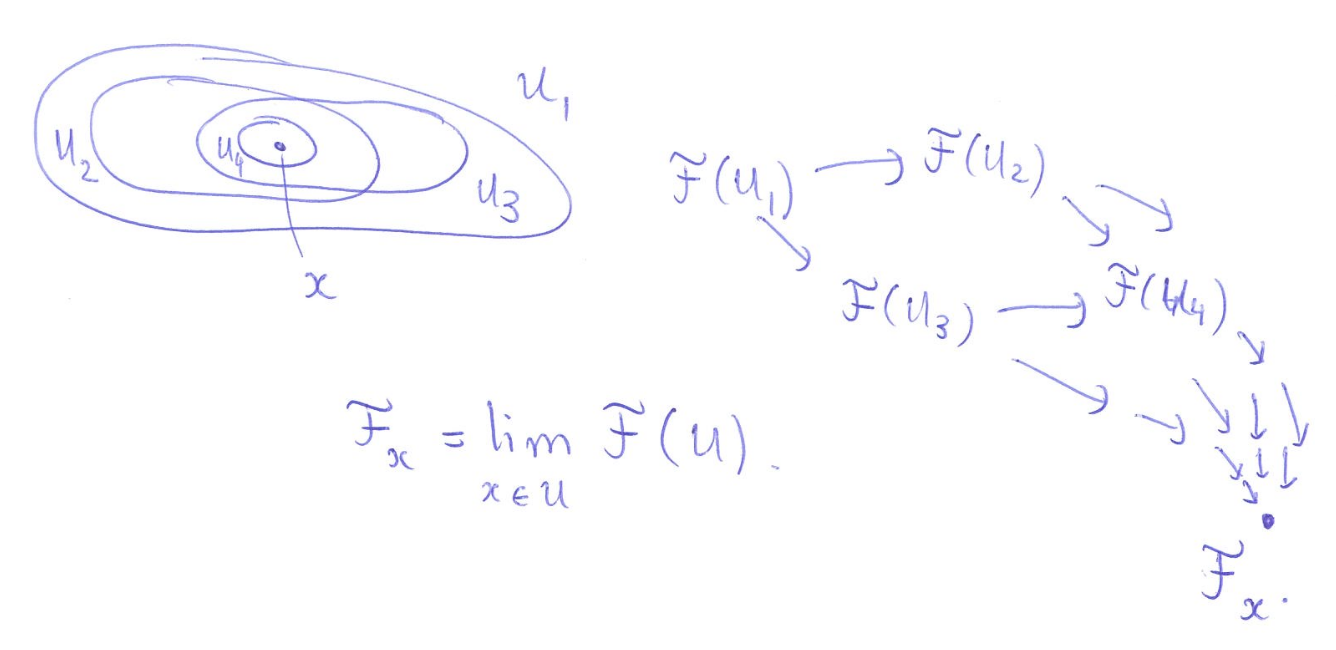
\includegraphics[width=100mm]{direct-limit.png}
\end{center}
{\color{red}Correct this diagram, it should read ``colimit''}. Elements of the stalk are called germs, and they consist of pairs $(U, s)$ where $U$ is an open containing $x$ and $s \in \CF(U)$. Two such pairs represent the same germ if there is an open subset of the intersection on which the restrictions of the sections coincide. Addition of germs $(V_1, s_1)$ and $(V_2, s_2)$ is carried out by restriction to $V_1 \cap V_2$ and addition of the sections $s_1$ and $s_2$ in $\CF(V_1 \cap V_2)$.

We recall the general definition of a colimit.
\begin{defn}
Let $J$ be a diagram in a category $\CC$, that is, a collection of objects $A_i \in \CC$ and a collection of morphisms $\al_{ij} : A_i \rightarrow A_j$. We consider the \emph{undercategory} which consists of tuples: $X \in \CC$ an object, and compatible $f_i : A_i \rightarrow X$ for each $A_i$ (compatible means $f_j \circ \al_{ij} = f_i$ whenever $\al_{ij} : A_i \rightarrow A_j$ is part of $J$). A colimit of $J$ is an initial object in the undercategory of $J$, that is, an object $(X, \{f_i\})$ such that for any other object $(X', \{f_i'\})$, there exists a unique morphism $X \rightarrow X'$ making a bunch of obvious diagrams commute.
\end{defn}
In this level of generality the colimit of a diagram may or may not exist. In the case of the collection of vector spaces $\CF(V)$ for $x \in V$ considered above, the colimit exists and is constructed as the vector space of germs described above.

%The most classic version of this construction is for functions: $\CF = \OO$.
%Example: The sheaf of germs of continuous functions on $X$. For $x \in X$ let $U \subset X$ be a neighbourhood of $x$ and $f$ a continuous function $U \rightarrow \R$. If we pass to smaller and smaller neighbourhoods

The set of stalks of a presheaf forms a sheaf. Indeed, starting with a presheaf $\CF$ on $X$ we are going to consider the disjoint union $\CF^+ = \bigcup_{x \in X} \CF_x$, and equip it with a topology such that it becomes a sheaf. The topology is the one generated by the following collection of open sets: for $U \subset X$ open and $s \in \CF(U)$ we define
\[
[U, s] = \{(x, s(x)) \mid x \in U\} \subset \CF^+.
\]
(See {\cite[Chap. II, Exercise 1.13]{Hartshorne}}.) The construction $\CF \mapsto \CF^+$ defines a functor, denoted $\Et$, or simply $(-)^+$.

Given a sheaf $\CF$ we can form a presheaf $\CF^\circ$ (my notation) by setting
\[
\CF^\circ(U) = \{f : U \rightarrow \CF \mid \text{$f(x) \in \CF_x$ and $f$ is continuous} \}.
\]
In fact the functors $(-)^+$ and $(-)^\circ$ are adjoint functors.

\begin{rem}
This definition of sheaf looks quite similar to the definition of a vector bundle over $X$. Recall that a vector bundle of finite rank $n$ consists of a total space $E$ with a projection $\pi : E \rightarrow X$ and certain homeomorphisms $\phi_U : \pi^{-1}(U) \rightarrow U \times \R^n$ (for $\{U\}$ some sufficiently fine cover of $X$) such that $\phi_U \circ \phi_V^{-1}$ are appropriately continuous on restrictions. In particular for every $x \in X$ there is the \emph{fibre} $\pi^{-1}(x) \cong \R^n$. On the other hand we have the set of sections
\[
\Gamma(U, E) = \{s : U \rightarrow \pi^{-1}(U) \mid \text{$s$ continuous and $\pi \circ s = 1_U$}\}.
\]
These vector spaces form a presheaf (denote it $\CF$), and we have the vector space $\CF_x$, the \emph{stalk} of $\CF$ at $x$. It is good to remember that the stalk and fibre are quite different. In fact the fibre at $x$ of our vector bundle is finite dimensional, while the stalk of the associated sheaf is the infinite dimensional vector space of ``germs of sections of $E$'' at $x$.
\end{rem}

The functors $(-)^+$ and $(-)^\circ$ are adjoint. It is customary (and probably more intuitive) to work in the category of presheaves, and define a sheaf according to some conditions which are always satisfied by presheaves of the form $\CF^\circ$. Explicitly
\begin{defn}
Let $\CF$ be a presheaf on $X$. We say $\CF$ is a sheaf if the following conditions hold:
\begin{itemize}
\item If $U \subset X$ is open and $\{V_i\}$ is an open cover of $U$, and we are given $s_i \in \CF(V_i)$ for each $i$, such that for all $i, j$
\[
\res_{V_i, V_i \cap V_j} s_i = \res_{V_j, V_i \cap V_j} s_j,
\]
then there exists $s \in \CF(U)$ such that
\[
s_i = \res_{U, V_i} s
\]
for each $i$.

\item If $s \in \CF(U)$ and $\{V_i\}$ is a cover as above, and $\res_{U, V_i} s = 0$ for each $i$, then $s = 0$. In particular the section $s$ whose existence is assured by the last item, is unique.
\end{itemize}
\end{defn}
The constant presheaf associated with vector space $M$ is not a sheaf. We define the \emph{constant sheaf} to be the sheafification of the constant presheaf, and we denote it $\underline{M}_X$. For all $x \in X$ the stalk of $\underline{M}_X$ at $x$ is a copy of $M$. Again, note that this is very different than the trivial vector bundle $E = X \times M$, whose \emph{fibre} (not stalk) at $x$ is a copy of $M$.

To see why the constant sheaf $\underline{M}_X$ is different than the constant presheaf $\CF$ defined by $\CF(U) = M$ for all open $U$, we consider $U \subset X$ the union of a collection of disjoint open sets $\{U_i\}$, and a section $v_i \in \CF(U_i)$ for each $i$. If the $v_i$ are not all equal, then there is no section in $\CF(U)$ which restricts to the various $v_i$. The stalk of $\CF$ at every point is $M$, so $\underline{M}_X = \CF^+$ is $X \times M$ with a certain weird topology, and the sheaf of sections $(\CF^+)^\circ$ turns out to be the set of locally constant $M$-valued functions on $X$.

The presheaf $C_X$ is already a sheaf, it turns out.

Another interesting example: Let $M$ be a fixed vector space, and $x \in X$ any point. We assign $\CF(U) = M$ for every open $U \subset X$ which contains $x$, and $\CF(U) = 0$ if not. We set $\res_{U, V} = \Id$ if $V$ contains $x$ and $0$ otherwise. This is a sheaf, and a sheaf of this form is known as a skyscraper sheaf on $X$.


In \cite{Hartshorne} (in the exercise referenced above), the topology on $\CF^+$ is described as being the ``strongest'' one for which the functions $U \rightarrow \CF^+$ defined by $x \mapsto (x, s(x))$ are continuous, for all open $U \subset X$ and all sections $s \in \CF(U)$. One topology is said to be ``stronger'' than another (or ``finer'' than another) if it contains all of the open sets of the latter. Thus the claim is plausible since the sets $[U, s]$ have been declared to be open, and if we were to declare any more sets to be open, it would become more difficult for a function $U \rightarrow \CF^+$ to be continuous.


A morphism of presheaves $\varphi : \CF \rightarrow \CG$ consists of the data of a morphism $\varphi_U : \CF(U) \rightarrow \CG(U)$ for each open $U$, which are compatible with the restriction maps in $\CF$ and $\CG$.

If we view a sheaf as a special kind of presheaf, then a morphism of sheaves is just a morphism of presheaves. If we adopt the fibre-wise definition then a morphism $\varphi : \CF \rightarrow \CG$ of sheaves consists of a morphism $\varphi_x : \CF_x \rightarrow \CG_x$ for each stalk, such that the union $\varphi : \CF \rightarrow \CG$ is continuous. We say that $\varphi$ is injective if each stalk map is injective, and surjective if each stalk map is surjective.

Translating the notions of injectivity and surjectivity back into the language of presheaves, we eventually find that $\varphi$ is injective/surjective exactly if: for every $x \in X$ there exists a neighbourhood $U$ of $x$ such that $\varphi_U : \CF(U) \rightarrow \CG(U)$ is injective/surjective.

Note that this definition is different than the following ``naive'' (and wrong) definition: a morphism of sheaves $\varphi : \CF \rightarrow \CG$ is injective/surjective if $\varphi_U : \CF(U) \rightarrow \CG(U)$ is injective/surjective for all open $U \subset X$. It's an exercise to show that an injective morphism of sheaves is always injective in this naive sense, but a surjective morphism is not necessarily surjective in the naive sense.

Regarding injectivity, the sheaf axiom used in an essential way. Indeed the idea is that if on some open $U$ the map $\varphi_U : \CF(U) \rightarrow \CG(U)$ were non injective, then the $\varphi_V$ would have to be non injective on some strictly smaller open $V \subset U$ because of the sheaf gluing axiom.

\begin{prop}
Let $X$ be a topological space. The category of all sheaves on $X$ is an abelian category, with kernel and cokernel defined stalk-by-stalk.
\end{prop}

Let $\CF$ be a sheaf on $X$ and $U \subset X$ an open subset. We have $\CF(U)$ which is just some vector space, and we have another entity $\CF|_{U}$ a sheaf on $U$ defined by
\[
\CF|_{U}(V) = \CF(V) \quad \text{for all $V \subset U$ open}.
\]


\begin{defn}
Let $M$ be a finite dimensional vector space. Let $\CF$ be a sheaf on $X$ such that for every $x \in X$ there exists a neighbourhood $U$ of $x$ and an isomorphism
\[
\CF|_U \cong \underline{M}_U.
\]
Then we say that $\CF$ is a local system on $X$.
\end{defn}

The constant sheaf is an obvious example of such a thing, but there are other examples too. Let $X = \C^\times = \C \backslash \{0\}$ and let
\[
\CF(U) = \{a x^{2/3} \mid a \in \C\}.
\]
The function $f(x) = x^{2/3}$ is not globally defined without a branch cut (in which case it becomes discontinuous across the cut). But in any sufficiently small ball we can define the function unambiguously, more precisely in
\[
B_\varepsilon(a) = \{x \in \C \mid |x-a| < \varepsilon\}
\]
for $a \in \C^\times$ and $0 < \varepsilon < |a|$.

We obtain a sheaf which is isomorphic to the constant sheaf $\underline{\C}_U$ when restricted to any of these balls, but which has no nonzero sections over $X$ and so is definitely not isomorphic to $\underline{\C}_X$.
% \begin{center}
% 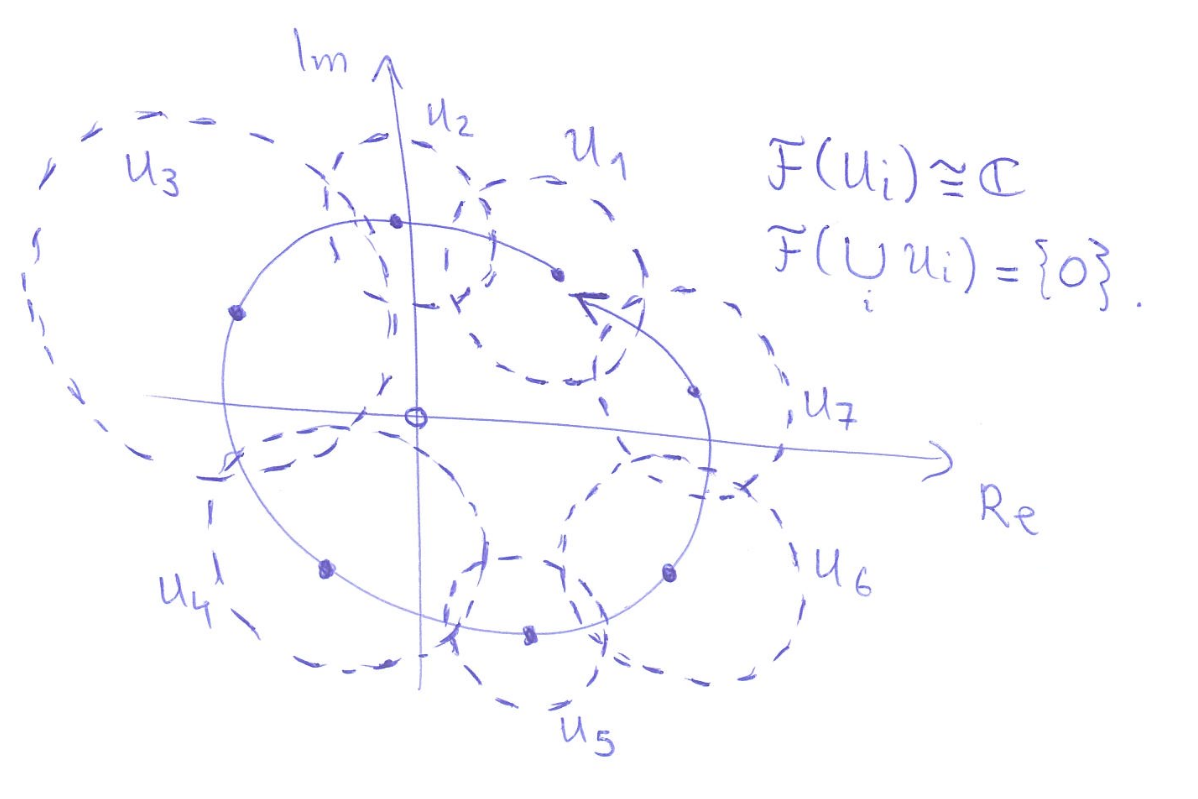
\includegraphics[width=100mm]{nontriv-loc-sys.png}
% \end{center}

\begin{figure}[htp]
\begin{center}
\begin{tikzpicture}[scale=1.5]
% Axes
\draw[->] (-2.5, 0) -- (2.5, 0) node[below right] {Re};
\draw[->] (0, -2.5) -- (0, 2.5) node[below right] {Im};

% Circles and points
\draw[dashed] (1, 0) circle (1/2);
\draw[dashed] (0.5, 0.866) circle (3/4);
\draw[dashed] (-0.5, 0.866) circle (1/2);
\draw[dashed] (-1, 0) circle (5/6);
\draw[dashed] (-0.5, -0.866) circle (3/5);
\draw[dashed] (0.5, -0.866) circle (2/3);
%\draw[dashed] (1.5, 0.866) circle (1);

% Dots at intersections
\draw (1.5, 0) node[above right] {$U_1$};
\draw (0.5, 0.866) node[above right] {$U_2$};
\draw (-0.5, 1.266) node[above left] {$U_3$};
\draw (-1, 0) node[above left] {$U_4$};
\draw (-0.5, -1.366) node[below left] {$U_5$};
\draw (1.2, -0.866) node[below right] {$U_6$};
%\draw (1.5, 0.866) node[above right] {$U_7$};
% Labels
% \node at (2.2, 1) {$F(U_i) \cong \mathbb{C}$};
% \node at (2.2, 0.5) {$F(\bigcup_i U_i) = \{0\}$};
\end{tikzpicture}
\end{center}
\caption{For each $i$ we have $\CF|_{U_i} = \underline{\C}_{U_i}$, while $\CF(\bigcup_i U_i) = \{0\}$}
\label{fig:1}
\end{figure}



{\color{red}GOT TO HERE ON 2024-01-18}

A comment on specifying a sheaf on a base. See {\cite[Section 6.30]{stacks-project}} for a careful discussion.
% https://stacks.math.columbia.edu/tag/009H
We recall that a topological space consists of a set $X$ and a set $\tau$ of subsets $U \subset X$ called the open subsets, such that $\tau$ satisfies certain axioms. By definition a \emph{base} of $\tau$ is a subset $B \subset \tau$ such that every $U \in \tau$ is equal to the union of a (possibly infinite) collection of sets in $B$. The open balls form a base of the usual metric topology of $\R^n$ for example.

To specify a sheaf it is sufficient to specify it on a base of the topology. If one wants to be formal, it is possible to define the notion of ``sheaf on $B$'' (where $B$ is a base of a topology), and then prove a proposition:
\begin{prop}
Let $\CF$ be a sheaf on a topological space $(X, \tau)$ with base $B$, then the restriction of $\CF$ to the open sets in $B$ defines a sheaf on the base, this operation defines a functor from the category of sheaves on $\tau$ to the category of sheaves on $B$, and this functor is an equivalence of categories.
\end{prop}



\section{Image functors of sheaves}


Let $X$, $Y$ be topological spaces, and $f : X \rightarrow Y$ a continuous function. Let $\CF$ be a sheaf on $X$. It is possible to push $\CF$ forward to $Y$ as follows: Let $V \subset Y$ be an open set, then $f^{-1}(V) \subset X$ is open, we define a presheaf $f_* \CF$ on $Y$ by
\[
f_*\CF(V) := \CF(f^{-1}(V)).
\]
One verifies that this is actually a sheaf.

The pushforward is always left exact, but not in general right exact. That is, let
\begin{align*}
0 \rightarrow \CF_1 \rightarrow \CF_2 \rightarrow \CF_3 \rightarrow 0
\end{align*}
be a short exact sequence of sheaves on $X$, then we claim that
\begin{align*}
0 \rightarrow f_*\CF_1 \rightarrow f_*\CF_2 \rightarrow f_*\CF_3.
\end{align*}
We have seen that injectivity/surjectivity can be tested by passing to a sufficiently small neighbourhood of each point. The thing is that no matter how small a neighbourhood $V$ of $y \in Y$ we take, the preimage $f^{-1}(V)$ might be ``big'', and so surjectivity of $f_*\CF_2(V) \rightarrow f_*\CF_3(V)$ might fail for \emph{all} neighbourhoods of $y$. The case of injectivity is different: An injection of sheaves really is injective on every open, and therefore injectivity of $\CF_1 \rightarrow \CF_2$ implies injectivity of $f_*\CF_1 \rightarrow f_*\CF_2$.

Now we describe pullback $f^{-1}\CG$ of a sheaf $\CG$ on $Y$. Since the image $f(U) \subset Y$ of open $U \subset X$ is not open in general, how to turn a presheaf on $Y$ into a presheaf on $X$ is not so clear. The definition, in fact, is the following: Let $\CG$ be a presheaf on $Y$, and let $U \subset X$ be open. Consider the set of all open $V \subset Y$ containing $f(U)$. We form a colimit\footnote{Remember: Initial object which receives maps from all the guys} over these, defining
\begin{align}\label{eq:pullback.presheaf}
f^{-1}\CG(U) = \colim_{V \supset f(U)} \CG(V).
\end{align}
If $\CG$ is a sheaf, then this construction is still not enough, as it happens that $f^{-1}\CG$ might not be a sheaf. So for sheaves $\CG$ on $Y$ we define $f^{-1}\CG$ to be the sheafification $(-)^+$ of the presheaf pullback described above.

The definition of pullback of a sheaf is actually easier if we use the stalk-wise definition. Then $\CG$ has a stalk $\CG_y$ at each $y \in Y$ and we define the sheaf $f^{-1}\CG$ to have stalk at $x$ given by $(f^{-1}\CG)_{x} = \CG_{f(x)}$.

It's an exercise to verify that the two definitions of the pullback of a sheaf coincide. We note that the pullback functor $f^{-1}$ is exact. This is transparent from the stalk-wise definition. See {\cite[Lemma 17.3.3(c)]{stacks-project}}.


It turns out $(f^{-1}, f_*)$ forms a left-right adjoint pair between categories of sheaves. Recall this means there are natural isomorphisms
\[
\Hom(f^{-1}\CG, \CF) \cong \Hom(\CG, f_*\CF).
\]
If we unpack what the two sides mean, the isomorphism becomes clear. This is a good exercise.
%
% \begin{exer}
% Do this!
% \end{exer}

Here is a little more explanation. A morphism $\CG \rightarrow f_* \CF$ consists of a compatible system of morphisms of vector spaces (indexed by open $V \subset Y$):
\[
\CG(V) \rightarrow f_*\CF(V) = \CF(f^{-1}(V)).
\]
Now we wish to describe morphisms $f^{-1}\CG \rightarrow \CF$. Since we have defined $f^{-1}(\CG)$ as a sheafification, we should comment on this before starting.
\begin{rem}[Thanks Diego!]
The sheafification functor $(-)^+$, and the functor $(-)^{\circ}$ sending a sheaf to its presheaf of sections (or rather, the functor of forgetting that the presheaf is a sheaf) is itself an example of an adjoint pair. Namely for any presheaf $\CF$ and sheaf $\CG$ on $X$, we have
\[
\Hom(\CF^+, \CG) \cong \Hom(\CF, \CG^{\circ}).
\]
\end{rem}
This means that to specify a morphism $f^{-1}\CG \rightarrow \CF$ of sheaves is really the same thing as to specify a morphism $f^{-1}\CG \rightarrow \CF$ where this time $f^{-1}\CG$ stands for the presheaf \eqref{eq:pullback.presheaf}. Such a morphism consists of a compatible system of morphisms of vector spaces (indexed by open $U \subset X$):
\[
\colim_{V \supset f(U)} \CG(V) \rightarrow \CF(U).
\]
Let us restrict to a fixed $U$ for a moment. By definition of colimit, a morphism as above is the same thing as a collection of compatible morphisms
\[
\CG(V) \rightarrow \CF(U)
\]
running over all open $V \supset f(U)$. Switching perspective and viewing $V$ as fixed, this is the data of a compatible system of morphisms running over all $U$ such that $f(U)$ is contained in $V$. But $f(U) \subset V$ is the same thing as saying $U \subset f^{-1}(V)$. Such a system is completely and uniquely determined by the morphism $\CG(V) \rightarrow \CF(f^{-1}(V))$. So we have proved the adjointness property. Moreover we have seen that at its core the adjointness of $(f^{-1}, f_*)$ hinges on the change of perspective between all open $V$ containing $f(U)$, and all open $U$ contained in $f^{-1}(V)$.


We reserve the symbol $\Gamma(X, -)$ for $\pi_*(-)$ the pushforward along the surjection $\pi : X \rightarrow *$ to a point. In other words $\Gamma(X, \CF)$ is $\CF(X)$. As for pushforwards in general, the functor
\[
\Gamma(X, -) : \sheaves(X) \rightarrow \Vect
\]
is left-exact. If we could show that $\sheaves(X)$ has enough injectives (which it does), then we could compute derived functors $R^n\Gamma(X, -)$.

Derived functors of pushforward to a point have a very natural interpretation. If $X$ is a sufficiently nice topological space they recover singular cohomology of $X$.
\begin{thm}\label{thm:sheaf-sing-coho}
Let $X$ be a topological manifold, then there are isomorphisms
\[
R^n\Gamma(X, \underline{\R}_X) \cong H_{\text{sing}}^n(X).
\]
\end{thm}
The theorem is true for topological spaces much more general than topological manifolds. It is true (for example) if $X$ is \emph{paracompact} and \emph{locally contractible}.

It's actually not hard to show that $\sheaves(X)$ has enough injectives, using a construction due to Godement.

Let $X$ be a topological space and let $\{M_x\}$ be a completely arbitrary collection of vector spaces indexed by $x \in X$. We define a presheaf $\CM$ by
\[
\CM(U) = \prod_{x \in U} M_x
\]
(so an element of this vector space is an arbitrary choice of $v_x \in M_x$ for each $x \in U$). This is easily seen to be a sheaf. One notes that the stalk $\CM_x$ of this sheaf at $x$ is very different from $M_x$.

Indeed consider the example in which $X = \R$ and $M_x = 0$ unless $x$ is of the form $1/n$ for $n \in \Z_{\geq 1}$, in which case $M_x = \C$. Then the stalk at $0$ is the vector space of ``tails'', namely the vector space of sequences
\[
(a_1, a_2, a_3, a_4, \ldots)
\]
modulo the equivalence relation $\sim$ that says
\[
(a_1, a_2, a_3, a_4, \ldots) \sim (b_1, b_2, b_3, b_4, \ldots)
\]
if there exists $N \geq 1$ such that $a_n = b_n$ for all $n \geq N$.


Given a sheaf $\CF$, one defines the Godement ``envelope'' of $\CF$ as the above construction applied to the collection of vector spaces $\CF_x$. There is a canonical morphism of sheaves
\[
\CF \rightarrow \Gode(\CF),
\]
indeed a section $s \in \CF(U)$ induces $s_x \in \CF_x$ at each $x \in U$, and we combine these to define a section $\widehat{s} \in \Gode(\CF)(U)$.

The construction described above (and so in particular the Godement envelope) is an example of an injective object in the category $\sheaves(X)$. Indeed let $i : \CF \rightarrow \CG$ be an injective morphism of sheaves, and let $\CM$ be a sheaf of the form described above: $\CM(U) = \prod_{x \in U} M_x$. Let a morphism $f : \CF \rightarrow \CM$ be given. By definition this consists of a collection of compatible morphisms
\[
\CF(U) \rightarrow \CM(U) = \prod_{x \in U} M_x,
\]
i.e., a collection of compatible morphisms
\[
\CF(U) \rightarrow M_x
\]
where $U$ runs over all open sets containing $x$. By definition of stalk this is the same thing as a morphism of vector spaces $\CF_x \rightarrow M_x$ (note: $M_x$ here, not $\CM_x$). Since vector spaces are always injective objects, we can extend this morphism along the injection $\CF_x \rightarrow \CG_x$ to obtain $\CG_x \rightarrow M_x$ for each $x$. It remains to confirm that these morphisms define a morphism of sheaves $\CG \rightarrow \CM$ making
\begin{align*}
\xymatrix{
\CF \ar@{^{(}->}[r]^{i} \ar@{->}[d]_{f} & \CG \ar@{-->}[dl]^{\wtil{f}} \\
%
\CM \\
}
\end{align*}


\begin{rem}
The world's shortest introduction to derived functors. The general narrative of derived functors starts from the notions of left and right exact functors. If the abelian category $\CC$ has enough projectives then any object $A \in \CC$ can be given a projective resolution $P_\bullet \rightarrow A$, and any such resolution can be used to compute the values on $A$ of the left derived functors $L_iF$ of a right exact functor $F$ (example: tensor product). Similarly if $F$ is left exact (example: $F(-) = \Gamma(X, -)$ from sheaves on $X$ to $\Vect$), then an injective resolution $A \rightarrow I^\bullet$ can be used to compute the values on $A$ of the right derived functors $R^iF$.
\end{rem}








{\color{red}GOT TO HERE ON 2024-01-22}

% It is also flabby (hence soft and acyclic).

Although it is important to know that enough projectives or enough injectives exist, in the day-to-day business of computing derived functors it is often possible to get away with using less exotic objects. Given a left exact functor $F$, there is a notion of $F$-injective object, and it is a theorem that a resolution by $F$-injective objects suffices to compute derived functors $R^iF$.

In the case of sheaves, one has the following notion:
\begin{defn}
A sheaf $\CF$ on $X$ is said to be flabby if the restriction morphism $\CF(X) \rightarrow \CF(U)$ is surjective for every open set $U \subset X$.
\end{defn}

It is then a standard theorem (I found it in these notes {\cite[Proposition 6.9]{Viterbo}}, look up a textbook reference)
\begin{thm}
A flabby sheaf is $\Gamma(X, -)$-injective, indeed $\Gamma(X, -)$-acyclic (which is stronger).
\end{thm}


The sheaves of singular cochains are not necessarily injective, but if $X$ is a topological manifold then they are flabby. So by the homological algebra general nonsense above, these sheaves can be used to resolve if one is computing global sections.

The proof of Theorem \ref{thm:sheaf-sing-coho} then proceeds by introducing sheaves of singular cochains. Roughly speaking: for $n \in \Z_{\geq 0}$ a basic singular chain in $U \subset X$ is a continuous function $\sigma : \D^n \rightarrow U$, where $\D^n$ is the standard $n$-simplex, and a singular chain is a formal linear combination of finitely many basic ones. The vector space of singular chains is denoted $C_n(U)$ and singular cochains are elements of $C^n(U) = C_n(U)^*$ the dual vector space. These form presheaves, which we then sheafify to obtain sheaves $\CC^n_{\text{sing}}$. The usual coboundary produces a complex
\[
0 \rightarrow \CC^0_{\text{sing}} \rightarrow \CC^1_{\text{sing}}\rightarrow \CC^2_{\text{sing}} \rightarrow \cdots
\]
of sheaves which resolves $\underline{\R}_X$ (this is proved by passing to small open sets in $X$ which are sufficiently nice to check explicitly). A key point is that the sheaves $\CC^n_{\text{sing}}$ are flabby, so the derived global sections of $\underline{\R}_X$ are computed as the cohomology of the complex of vector spaces
\[
0 \rightarrow \Gamma(X, \CC^0_{\text{sing}}) \rightarrow \Gamma(X, \CC^1_{\text{sing}}) \rightarrow \Gamma(X, \CC^2_{\text{sing}}) \rightarrow \cdots
\]
Now these vector spaces are exactly the vector spaces of singular cochains which are used to define singular cohomology in basic topology.





\section{Weyl character formula}


Where we left off our study of category $\OO$, we had seen that every $M \in \OO$ possesses a composition series with factors a finite set of irreducible modules $L(\la_i)$, each with a finite multiplicity $b_i \in \Z_{\geq 0}$. These factors and multiplicities are independent of the specific composition series, so we write $[M : L(\la)]$ for $b_i$. This induces an equality of characters
\[
\ch_M = \sum_{\la_i} m_i \ch_{L(\la_i)}.
\]

We are particularly interested in the multiplicities
\[
b_{\La, \la} = [M(\La) : L(\la)]
\]
(where $\La \in P$ for simplicity). We know that $L(\La)$ appears as the first quotient $M(\La) / J$, so $b_{\La, \La} = 1$. Then any other nonzero $b_{\La, \la}$ occur for $\la < \La$. Let us choose a linear order on $P$ consistent with the partial order $\leq$. The set of coefficients
\[
b_{\La, \la} = [M(\La) : L(\la)]
\]
can be viewed as a $\Z \times \Z$ matrix, which is lower triangular with ones on the diagonal. Hence the matrix can be inverted and we may write
\begin{align} \label{lfromm}
\ch_{L(\La)} = \sum_{\la \leq \La} m_{\La, \la} \ch_{M(\la)}.
\end{align}
We have $m_{\La, \La} = 1$ and $m_{\La, \la} \in \Z$.







We will prove a formula for the character of $L(\La)$ for $\La \in P_+$.

Combining the formula for the character of the Verma with equation \eqref{lfromm} and multiplying through by $e^\rho$ yields
\begin{align} \label{wkp-pre}
R \ch_{L(\La)} = \sum_{\la \leq \La} m_{\La, \la} e^{\la}, \qquad R = \prod_{\al \in \D_+} (1-e^{-\al}).
\end{align}
For reasons that will become clear soon, we will multiply through to obtain:
\begin{align} \label{wkp}
e^\rho R \ch_{L(\La)} = \sum_{\la \leq \La} m_{\La, \la} e^{\la+\rho}.
\end{align}

%To go further we either need some more assumptions on our module, or some more heavy theory.

First we will show that $e^\rho R$ is $W$-skew invariant by checking it on the generating reflections $r_i$. We need the following two facts:
\begin{itemize}
\item $\D$ is $W$-invariant.

\item The set $\D_+ \backslash \{\al_i\}$ is invariant under $r_i$.
\end{itemize}
The first fact is part of the classical theory we reviewed in the first lessons.

As for the second fact: write $\beta \in \D_+ \backslash \{\al_i\}$ as a $\Z_+$-linear combination of the $\al_k$ with a positive coefficient for some simple root $\al_j \neq \al_i$. Then $r_i(\beta)$ also has a positive coefficient of $\al_j$ and hence lies in $\D_+ \backslash \{\al_i\}$, because every root is either positive or negative.

Now we calculate
\begin{align*}
r_i(e^\rho R)
%
= e^{\rho-\al_i} (1 - e^{\al_i}) \prod_{\al \in \D_+ \backslash \{\al_i\}} (1 - e^{-\al})
%
= -e^\rho R,
\end{align*}
which is the $W$-skew invariance asserted above.

We have assumed that $\La \in P_+$. We now show that this implies $\ch_{L(\La)}$ is $W$-invariant.
\begin{defn}
Let $\g$ be semisimple. A weight module for $\g$ is said to be \emph{integrable} if $E_{\al}$ acts locally nilpotently in $M$ for all $\al \in \D$.
\end{defn}
Let $M$ be integrable and let $\mu \in \supp(M)$. For some simple root $\al$, consider the $\sll_2$-subalgebra $\ma = <E_\al, \al^\vee, E_{-\al}>$ and its representation in $L = \bigoplus_{n \in \Z} M_{\la + n \al}$. Because of integrability, each vector in $L$ lies in a finite dimensional $\ma$-submodule. By an argument similar to the one we did for $\g$ itself, we may deduce that each weight space of $L$ is finite dimensional and
\[
\dim(M_\la) = \dim(M_{r_i(\la)}).
\]
The $W$-invariance of $\ch_{M}$ follows.
\begin{lemma}
If $\La \in P_+$ then $L(\La)$ is integrable.
\end{lemma}

\begin{proof}
We know that $\n_+$ acts locally nilpotently, since we checked $L(\La)$ is in $\OO$. Now check that local nilpotence of $\n_-$ holds on the highest weight vector $v_\La$. The idea now is to prove local nilpotence on other vectors inductively.
\end{proof}

An immediate corollary of $W$-invariance of the character is finite dimensionality of $L(\La)$, which we asserted without proof in Theorem \ref{thm:P+.implies.fin.dim}.

We now see that
\[
\sum_{\la \leq \La} m_{\La, \la} e^{\la+\rho}
\]
must be $W$-skew invariant.

Consider a weight $\la$ such that $m_{\La, \la} \neq 0$. If $w(\la+\rho) = \mu+\rho$ then $m_{\La, \la} = \eps(w) m_{\La, \mu}$ because of skew invariance. Because $m_{\La, \la} \neq 0$ only for $\la \leq \La$ we deduce that $w(\la+\rho) \leq \La+\rho$ for all $w \in W$.

Next we will show that the range of summation in (\ref{wkp}) is $\la \in W \circ \La$, where $\circ$ is the \emph{shifted action} of the Weyl group $w \circ \la = w(\la+\rho)-\rho$. In fact it follows from Proposition \ref{prop:block-condition}. We now give a proof for $\La \in P_+$ (the only case we need here).
\begin{prop}\label{prop:dominant-block-condition}
Let $L(\la)$ be a composition factor of $M(\Lambda)$, where $\La \in P_+$. Then $\la \geq \La$ and
\[
\la = w(\La+\rho) - \rho
\]
for some $w \in W$.
\end{prop}


\begin{proof}
Let $\mu = w\circ \la$ be such that $\height(\La-\mu)$ takes its minimal value as $w$ ranges over $W$. We will prove that $\mu = \La$. First we will prove that $\mu \in P_+$. Indeed if $\left<\mu+\rho, \al^\vee_i\right> < 0$ for some $i$ then
\[
\La - r_i \circ \mu = \La+\rho - r_i(\mu+\rho) = \La-\mu + \left<\mu+\rho, \al^\vee_i\right> \al_i
\]
has strictly lower height than $\La-\mu$. Hence $\left<\mu+\rho, \al^\vee_i\right> \geq 0$ for each $i$, which is to say
\[
\mu+\rho \in P_+.
\]

Now, $\La+\rho$ and $\mu+\rho$ are in $P_+$ and $(\La+\rho) - (\mu+\rho) = \sum_i k_i \al_i$ where all $k_i \geq 0$. Also $|\La+\rho|^2 = |\mu+\rho|^2$, which implies
\[
0 = |\La+\rho|^2 - |\mu+\rho|^2 = (\La+\mu+2\rho, \La-\mu) = \sum_i k_i \left<\La+\mu+2\rho, \al^\vee_i\right> (\al_i, \al_i).
\]
The terms in the summation on the right are all positive, so each $k_i = 0$ in fact, hence $\mu = \La$.

It follows that $\la \in W \circ \La$, as claimed.
\end{proof}

We have shown that
\[
R \ch L(\La) = \sum_{\la \in W \circ \La} m_{\La, \la} e^{\la}.
\]
There is one more step to the final version:
\begin{thm}[Weyl-Kac]
Let $\La \in P_+$, then
\begin{align} \label{wk}
R \ch L(\La) = \sum_{w \in W} \eps(w) e^{w \circ \La}.
\end{align}
\end{thm}

To complete the proof we just need to show that the stabiliser of $\La$ in $(W, \circ)$ is $\{1\}$.% This fact is actually true for all $\la$ such that $\la+\rho \in P_{++}$.

%REMARK: I'm not completely sure why this fact is necessary: the LHS is skew-invariant, therefore so is the RHS. we also know that $m_{\La, \La} = 1$, so choose $w \in W$ taking $\La$ to $\la$, we deduce that $m_{\La, \la} = \eps(w)$. If two $w$ of different parities map $\La$ to $\la$ then so be it! This is a contradiction and all that means is that the assumptions we have made so far on $\La$ are incompatible with this possibility.

%In fact it looks like people exploit this already.


%\subsection{The dominant integral weights form a fundamental domain for $W$}

\begin{prop}\label{prop:P+.trivial.stab}
Let $\La \in P_+$, then the stabiliser of $\La$ under the dot action of $W$ is trivial.
\end{prop}

The proof relies on an annoyingly complicated lemma about the geometry of the $W$-action on $\h^*$. But the lemma will be needed later on too, so we should take it seriously.
\begin{lemma} \label{lem:comb}
If $r_{i_1} \cdots r_{i_t}(\al_i) < 0$ then there exists $s$ ($1 \leq s \leq t$) such that
\[
r_{i_1} \cdots r_{i_s} \cdots r_{i_t} r_i = r_{i_1} \cdots r_{i_{s-1}} r_{i_{s+1}} \cdots r_{i_t}.
\]
\end{lemma}

\begin{proof}
For each $ k < t$ let $\beta_k = r_{i_{k+1}} \cdots r_{i_t}(\al_i)$, and let $\beta_t = \al_i$. By hypothesis $\beta_0 < 0$, and $\beta_t > 0$.

Let $\beta_{s-1} < 0$, $\beta_s > 0$, we have $\beta_{s-1} = r_{i_s} \beta_s$. Now, if $\beta \in \D_+$, then $(\beta + \Z \al_k) \cap \D \subseteq \D_+$ unless $\beta = \al_i$ simply because every root is either positive or negative. Therefore if $\beta \in \D_+$ and $r_i(\beta) < 0$ then $\beta = \al_i$. Applying this to the situation at hand shows that $\beta_s = \al_{i_s}$. Also $\al_{i_s} = w(\al_i)$ where $w = r_{i_{s+1}} \cdots r_{i_t}$.

The subspaces $\R \al_i$ and $\al_i^\perp$ are complementary, and $r_i$ is the unique linear transformation that sends $\al_i$ to $-\al_i$ and restricts to the identity on $\al_i^\perp$. The same goes for $\al_{i_s}$. Because $w$ is an orthogonal transformation sending $\al_i$ to $\al_{i_s}$, it sends $\al_i^\perp$ to $\al_{i_s}^\perp$. Therefore $r_{i_s} = w r_i w^{-1}$.

Substituting this for $r_{i_s}$ into $r_{i_1} \cdots r_{i_s} \cdots r_{i_t} r_i$ yields $r_{i_1} \cdots r_{i_{s-1}} r_{i_{s+1}} \cdots r_{i_t}$ as desired.
\end{proof}



\begin{proof}[Proof of Proposition \ref{prop:P+.trivial.stab}]
Now, $A$ is an integer matrix, so we could have defined $\h_\R$ and $\h_\R^*$, using $\R$ in place of $\C$. We can embed $\h_\R \hookrightarrow \h$. The action of $W$ may be defined on $\h_\R^*$ since the definition makes no reference to the base field.

Let
\[
\h_\R^\circ = \{h \in \h_\R | \text{$\left<\al, h\right> \neq 0$ for each $\al \in \D$}\}.
\]
The \emph{positive (open) Weyl chamber} is the set
\[
C = \{h \in \h_\R | \text{$\left<\al_i, h\right> > 0$ for each $i$}\}.
\]
% The Tits cone is $X = \cup_{w \in W} w(C)$, $C^\vee, X^\vee \subseteq \h_\R^*$ are defined similarly.

We claim that $C$ is a fundamental domain for the action of $W$ on $\h_\R^\circ$, i.e., for all $h \in C$, $w(h) = h$ if an only if $w = 1$. The claim above about $P_{+}$ will follow.



Suppose now that $h \in C$ and $h' = w(h) \in C$ also. Let $w = r_{i_1} \cdots r_{i_t}$ be a \emph{reduced expression} for $w \neq e$, meaning that $t \in \Z_{>0}$ is minimal among all possible such representations of $w$. We have $\left<\al_{i_t}, h\right> > 0$ by hypothesis, therefore $\left<w(\al_{i_t}), w(h)\right> = \left<w(\al_{i_t}), h'\right> > 0$ too.

On the other hand we claim that $w(\al_{i_t}) \in \D_-$. For assume it were the case that $w(\al_{i_t}) \in \D_+$, then we would have
\[
r_{i_1} \cdots r_{i_{t-1}}(\al_{i_t}) = w r_{i_t}(\al_{i_t}) = w(-\al_{i_t})\in \D_-,
\]
and it would follow from Lemma \ref{lem:comb} that our expression for $w$ was not reduced, a contradiction.

Therefore $\left< w(\al_{i_t}), h' \right> < 0$, which contradicts $h' = h$. So $w = e$.
\end{proof}


The proof contains a result which it will be useful to state on its own.
\begin{lemma}\label{lem:reduced.expression.lemma}
Let $w \in W$ of length $\ell(w) = k$. Then there exists $i$ such that $w r_i$ has length $k-1$. Furthermore
\[
w(\al_i) \in \D_- \qquad \text{and} \qquad (wr_i)(\al_i) \in \D_+.
\]
\end{lemma}

Exercise: Write out a proof.




{\color{red}GOT TO HERE ON 2024-01-24}



\section{Category $\OO$ has enough projective}


Let us finally prove the following classification of indecomposable objects in a block of category $\OO$ for $\sll_2$.
\begin{prop}
Let $\g = \sll_2$. There are exactly $5$ indecomposable objects in the block $\OO_0$, and they are the following:
\begin{itemize}
\item The Verma $M = M(0)$ and its irreducible quotient $L = L(0)$,

\item The dual Verma $M^\vee$,

\item The irreducible Verma $M^- = M(-2\varpi)$ (which is self-dual),

\item The module $V$ constructed in the first exercise list as an extension
\[
0 \rightarrow M \rightarrow V \rightarrow M^- \rightarrow 0.
\]
\end{itemize}
\end{prop}


\begin{proof}
Let $A \in \OO_0$ and consider the submodule $B = U(\g)A_0 \subset A$. We claim that $B$ is isomorphic to a direct sum of copies of $M$ and $L$. Indeed let $v_1 \in A_0$ be nonzero and $B^1 = U(\g)v_1 \subset B$.

Since $v_1$ is a singular vector, there is a surjection $M \rightarrow B^1$ and so $B^1$ is either isomorphic to $M$ or else to its unique nontrivial quotient $L$.

Now grab another vector $v_2 \in A_0$ and consider the submodule $B^2$ generated by $v_1$ and $v_2$. (We could consider the submodule generated by $v_2$ alone, but that might have nontrivial intersection with $B^1$, and things would quickly get complicated). We can say that $B^2 \supset B^1$ with both $B^1$ and $B^2 / B^1$ isomorphic to $L$ or to $M$. In other words we have an extension
\[
0 \rightarrow B^1 \rightarrow B^2 \rightarrow B^2/B^1 \rightarrow 0
\]
which is of the following four:
\begin{align*}
0 &\rightarrow L \rightarrow E \rightarrow L \rightarrow 0 \\
%
0 &\rightarrow M \rightarrow E \rightarrow M \rightarrow 0 \\
%
0 &\rightarrow L \rightarrow E \rightarrow M \rightarrow 0 \\
%
0 &\rightarrow M \rightarrow E \rightarrow L \rightarrow 0.
\end{align*}
Since $L$ is finite dimensional, we know that there are no nontrivial extensions of $L$ by $L$, so in that case $B^2$ would be a direct sum of two copies of $L$.

The middle two cases are also easy to treat. In fact we have a general lemma:
\begin{lemma}
Let
\begin{align*}
0 \rightarrow A \rightarrow E \rightarrow M(\lambda) \rightarrow 0
\end{align*}
be an extension, where
\[
\supp(A) \subset \supp(M(\la)).
\]
Then the extension is split.
\end{lemma}

\begin{proof}
Let $e_\la \in E_\la$ be a preimage in $E$ of the generating vector $v_\la \in M(\la)$. Because of the condition on supports, $e_\la$ is a singular vector in $E$ and so by the universal property, there exists a morphism $\al : M(\la) \rightarrow E$ sending $\al(v_\la) = e_\la$. The image of $\al$ is some quotient of $M(\la)$. But since $e_\la \mapsto v_\la$ in the exact sequence, the image of $\al$ must surject to $M(\la)$ and so $Im(\al) \subset E$ is a copy of $M(\la)$. We have just described a splitting of the exact sequence.
\end{proof}

What about the final case? Now there is no general result to appeal to, but we can analyse this specific case as follows. We know that
\[
0 \rightarrow N \rightarrow M \rightarrow L \rightarrow 0,
\]
where $N$ in this case is the Verma module $M^-$. Observe that $\Hom(N, M) \cong \C$ since the weight spaces are all $1$-dimensional.

Now we will use this SES to get a LES for $\Ext$ (Derived functors of Homming to $M$), namely
\begin{align*}
\xymatrix{
 &  &  \\
%
\Ext(N, M) \ar@{->}[urr] & \Ext(M, M) \ar@{->}[l] & \Ext(L, M) \ar@{->}[l] &  \\
%
\Hom(N, M) \ar@{->}[urr] & \Hom(M, M) \ar@{->}[l] & \Hom(L, M) \ar@{->}[l] & 0  \ar@{->}[l] \\
}
\end{align*}
What we know so far is that
\begin{align*}
\xymatrix{
 & 0 \ar@{->}[l] & (?) \ar@{->}[l] &  \\
%
\C \ar@{->}[urr] & \C \ar@{->}[l]^{\cong} & 0 \ar@{->}[l] & 0  \ar@{->}[l] \\
}
\end{align*}
and exactness of the LES gives us $\Ext(L, M) = 0$.

So now we know in all cases that $B^2$ is a direct sum of copies of $L$ and/or $M$. We continue inductively (using that $\Ext$ spaces are additivie in their arguments). So $B \subset A$ is a direct sum of copies of $L$ and $M$.

Consider now $Q = A / B$. The submodule $C$ of $Q$ generated by $Q_{-2}$ must be isomorphic to a direct sum of copies of $M^-$ (same reasoning as above, but simpler this time). In fact $Q = C$ as there are no further irreducible modules in $\OO_0$ beyond $L$ and $M^-$ to form its composition series.

Now we either have $A$ isomorphic to a direct sum of copies of $L$, $M$ and $M^-$, or else $A$ contains a nontrivial extension
\[
0 \rightarrow L \rightarrow U \rightarrow M^- \rightarrow 0.
\]
or
\[
0 \rightarrow M \rightarrow V \rightarrow M^- \rightarrow 0.
\]
There is a unique up to isomorphism extension $U$, and it is actually $M^\vee$. This can be proved by hand, similarly to the exercise proving uniqueness of the extension $V$.

Now we make a key observation: As we have proved in a previous lecture,  $M$ is a projective module, and so $M^\vee$ is an injective module. This means that if $M^\vee$ occurs as a submodule of $A$ then it occurs as a summand. So we can consider the other summand and proceed inductively.

In fact if we could show that $V$ is injective then we would be finished. In fact it is, as we show in the next proposition.
\end{proof}

\begin{prop}
The extension $V$ is injective.
\end{prop}

\begin{proof}
First we note that $V^\vee \cong V$, so it suffices to show that $V$ is projective. Indeed consider these pictures

INSERT


To prove projectivity, we will reduce it to a general result using a clever realisation of $V$. Consider the Verma module $M(-\rho) = M(-\varpi)$. This module has the special property of being the unique Verma module in its block $\OO_{-\rho}$. Since $L(-\rho) = M(-\rho) / J$ where the composition factors of $J$ must have strictly lower weight, in fact $J = 0$ and $M(-\rho)$ is irreducible.

Because there are no Verma modules of weight higher than $-\rho$ in the same block either, we conclude that $M(-\rho)$ is projective.

Now we consider $M(-\varpi) \otimes L(\varpi)$, it is isomorphic to $V$! Since $L(\varpi)$ is finite dimensional, it follows that $V$ is projective by Proposition \ref{prop:tensor.fin.dim} below.
\end{proof}


\begin{prop}\label{prop:tensor.fin.dim}
If $P \in \OO$ is projective, and $L$ is finite dimensional, then $P \otimes L$ is projective.
\end{prop}


\begin{proof}
Recall that projectivity of $P$ means (by definition, essentially) that the functor
\[
X \mapsto \Hom(P, X)
\]
is exact. But now
\begin{align*}
X \mapsto &\Hom(P \otimes L, X) \\
%
&\cong \Hom(P, \Hom(L, X)) \\
%
&\cong \Hom(P, X \otimes L^*)
\end{align*}
is exact too.
\end{proof}




Now let us discuss embeddings of Verma modules, tying up with the notion of reduced expressions in the Weyl group.
\begin{prop}\label{prop:length.embeddings}
Let $w = r_{i_t} \cdots r_{i_1}$ be a reduced expression, and write $w^{(k)} = r_{i_{k}} \cdots r_{i_1}$ (so $w^{(0)} = e$, $w^{(1)} = r_{i_1}$ and $w^{(t)} = w$). Suppose that $\La \in P_+$. Then there exists an embedding
\[
M(w^{(k)} \circ \La) \rightarrow M(w^{(k-1)} \circ \La)
\]
for each $k \geq 1$.
\end{prop}


\begin{proof}
We wish to show that
\begin{align*}
m = \left< w^{(k-1)} \circ \La, \al_{i_k}^\vee \right> \in \Z_{\geq 0},
\end{align*}
for it then follows that
\[
F_{i_k}^{m+1} v_{w^{(k-1)} \circ \La}
\]
is a singular vector.

But we compute
\begin{align*}
\left< w^{(k-1)} \circ \La + \rho, \al_{i_k}^\vee \right>
%
&= \left< w^{(k-1)} (\La + \rho), \al_{i_k}^\vee \right> \\
%
&= \left< \La + \rho, (w^{(k-1)})^{-1}(\al_{i_k}^\vee) \right> \\
%
&= \left< \La + \rho, r_{i_{1}} \cdots r_{i_{k-1}}(\al_{i_k}^\vee) \right> \\
%
&= \left< \La + \rho, \beta \right>
\end{align*}
where $\beta \in \D_+$, by Lemma \ref{lem:comb}. The expression is therefore positive, and we are done.

The fact that $M(w^{(k)} \circ \La) \rightarrow M(w^{(k-1)} \circ \La)$ is injective is the following lemma.
\end{proof}




{\color{blue}I DREW A BUNCH OF PICTURES OF INCLUSIONS OF VERMAS FOR SL3. DRAW THEM AND INCLUDE THEM HERE.}

From Lemma \ref{lem:comb} and Proposition \ref{prop:length.embeddings} we start to perceive the surprising importance of reduced expressions in the Weyl group $W$ of a simple Lie algebra $\g$. In particular we give the symbol $\ell$ to the function
\[
\ell : W \rightarrow \Z_{\geq 0}
\]
sending $w \in W$ to the length of any reduced expression of $w$. The length function has other combinatorial interpretations. Later we shall see:
\begin{prop}\label{prop:wD+D-ell}
For all $w \in W$ one has
\[
\ell(w) = |w(\D_+) \cap \D_-|.
\]
\end{prop}
From this it follows immediately that $0 \leq \ell(w) \leq |\D_+|$ for all $w \in W$. In fact the maximal value of $|\D_+|$ is realised by, it turns out, a unique element in the Weyl group. This element is denoted $w_\circ$ and is simply called ``the longest element'' of the Weyl group.

Another curious element of $W$ is the so-called \emph{Coxeter element}. This is the product of all the simple reflections, taken in any random order, each exactly once. It turns out this element is well-defined up to conjugacy. Its order is a number
\[
h
\]
called the \emph{Coxeter number} of $\g$. For example $h(\sll_n) = n$ and $h(E_8) = 30$.


Another important number associated with $\g$ is the \emph{dual Coxeter number} $h^\vee$, which is defined as follows: let $\theta \in \D_+$ be the highest root (the unique root such that no root is higher than it) and let $\kappa$ denote the Killing form of $\g$ (which we restrict to $\h$, use to identify $\h \rightarrow \h^*$, and finally transfer to a bilinear form $\kappa$ on $\h^*$), then
\[
\kappa(\theta, \theta) = \frac{1}{h^\vee}.
\]
It is very common to define
\[
(\lambda, \mu) = 2 h^\vee \kappa(\la, \mu),
\]
so that $(\theta, \theta) = 2$.

Some weird relations satisfied by $h$ and $h^\vee$:
\[
h = \frac{\dim(\g)}{rank(\g)}
\]
and
\[
|\rho|^2 = \frac{h^\vee \dim(\g)}{12}.
\]





{\color{red}GOT TO HERE ON 2024-01-25}


Finally we will use Proposition \ref{prop:tensor.fin.dim} to show that $\OO$ has enough projectives. For this we will need a lemma which will be useful on its own too.
\begin{lemma}[{\cite[Theorem 3.6]{humbgg}}]\label{lem:Verma.filtration}
Let $\lambda \in \h^*$ and let $L$ be a finite dimensional $\g$-module. Then the tensor product
\[
M(\lambda) \otimes L
\]
carries a filtration, whose associated graded is a direct sum
\[
\bigoplus_{\nu} M(\lambda+\nu)
\]
of Verma modules, where $\nu$ runs over the weights of $L$ counted with multiplicity.
\end{lemma}

\begin{proof}
Consider the isomorphism
\[
(U(\g) \otimes_{U(\fb)} W) \otimes L \cong U(\g) \otimes_{U(\fb)} (W \otimes L),
\]
here on the left we have a tensor product of $U(\g)$-modules, and on the right we are considering $L$ as a $U(\fb)$-module by restriction. The case of interest is $W = \C v_\la$, for which the left hand side is $M(\la) \otimes L$.

Since $W$ and $L$ are weight modules, so is $W \otimes L$. We choose a basis $\{v_1, \ldots, v_n\}$ ordered so that $i \leq j$ whenever $\wt(v_i) \leq \wt(v_j)$ (so $v_n$ is the highest of the weights). Since the action of $\fb$ only raises weights, the span of the subset of vectors $\{v_k, \ldots, v_n\}$ is a $\fb$-submodule of $W \otimes L$ for each $k$. In other words we have a filtration
\[
W \otimes L = N_1 \supset N_2 \supset \ldots \supset N_n \supset N_{n+1} = 0,
\]
with $N_k$ being the span of $\{v_k, \ldots, v_n\}$. The associated graded is a direct sum of one-dimensional weight modules $\C v_{\la+\nu}$ where $\nu$ runs over the weights of $L$.

Since the functor
\[
U(\g) \otimes_{U(\fb)} (-)
\]
is exact, the $\g$-module
\[
U(\g) \otimes_{U(\fb)} (W \otimes L)
\]
carries a filtration whose associated graded is a direct sum of modules $M(\la+\nu)$. This completes the proof.
\end{proof}

The following proposition is Theorem 3.8 of the book \cite{humbgg} of Humphreys.
\begin{thm}
Let $\g$ be a semisimple Lie algebra. Then the category $\OO$ has enough projectives and enough injectives.
\end{thm}


\begin{proof}
We shall prove that $\OO$ has enough projectives, that is, that for every $M \in \OO$ there exists a projective object $P$ and a surjection $P \rightarrow M$. By considering contragredient objects we will conclude that $\OO$ has enough injectives too.

Let $M(\la)$ be a Verma module. There exists some $\La = \la + N \rho$ for which $M(\La)$ is projective, so consider $M(\La) \otimes L(N\rho)$ which is also projective since $L(N\rho)$ is finite dimensional. We take an ordered basis of $L(N\rho)$ with weights increasing, as recommended in the lemma above. The first vector lies in weight $-N\rho = w_\circ(N\rho)$. The lemma then tells us that the first quotient in the filtration of $M(\La) \otimes L(N\rho)$ is a copy of $M(\La-N\rho) = M(\la)$. Thus we have proved that $M(\la)$ receives a surjection from the projective object $M(\La) \otimes L(N\rho)$.

Since every irreducible in $\OO$ is $L(\la)$ for some $\la$, it follws that all irreducibles receive a surjection from a projective. By induction on the length of a composition series it is possible to extend this result to all objects of $\OO$. See the proof in \cite{humbgg} for details, or better yet, reconstruct them for yourself.
\end{proof}


Let us finish up this section with a few other useful facts about Verma modules which do not need any special theoretical machinery to prove.
\begin{lemma}
Any nonzero morphism $M(\mu) \rightarrow M(\la)$ is injective.
\end{lemma}

\begin{proof}
As $U(\n_-)$-modules we have $M(\mu) \cong M(\la)$, and $M(\mu) \rightarrow M(\la)$ is of the form $u \mapsto u u_0$ for some (nonzero) $u_0 \in U(\n_-)$. But the ring $U(\n_-)$ has no zero divisors, so $u u_0 = 0$ only if $u = 0$ and we are done.
\end{proof}


\begin{lemma}
For any weights $\la$, $\mu$ we have
\[
\dim \Hom(M(\mu), M(\la)) \leq 1.
\]
\end{lemma}

\begin{proof}
First we claim that any Verma module possesses a unique irreducible submodule. In fact the ring $U(\n_-)$ is left Noetherian, and the statement follows from a general argument about Noetherian rings. Namely: if $x \neq 0$ is a non-right-zero-divisor and $I$ a left ideal in the left Noetherian ring $R$, then $Rx$ meets $I$ nontrivially. Indeed the chain of ideals
\[
I \subset I + Ix \subset I + Ix + Ix^2 \subset \ldots
\]
must stabilise, so forsome $N$ we have
\[
x^N = a_0 + a_1 x + \cdots + a_{N-1} x^{N-1}, \qquad a_i \in I.
\]
Assume $I \cap Rx = 0$. Then from the equation we have $a_0 = 0$. But then we can cancel $x$ from the equation and also deduce $a_1 = 0$, and continue in this way until we find $x = 0$, which is a contradiction. So in fact $Rx$ has nonzero intersection with every left ideal in $R$. It follows, in fact, that every pair of nonzero left ideals has nonzero intersection.

Applied to $R = U(\n_-)$: Suppose there were two distinct irreducible submodules of $M(\la) \cong U(\n_-)$, corresponding to distinct left ideals $I_1$ and $I_2$. They have nonzero intersection, but the intersection is a $\g$-submodule (Think about why!) and so both submodules must be equal to it, and to each other.

Now we turn to the proof of the lemma. Let $f_1$, $f_2$ be two such morphisms. Each of them sends the unique irreducible submodule $S \subset M(\mu)$ to some (irreducible) submodules $S_1$, $S_2$ of $M(\la)$. Again by uniqueness, these images coincide, and so there exists some constant $c$ for which $f_1 = c f_2$. But then $g = f_1 - cf_2$ by construction satisfies $g(S) = 0$, and so by the previous lemma, $g = 0$.
\end{proof}





\section{Lie groups and algebraic groups}


A Lie group is a smooth manifold $G$ which is simultaneously a group in the sense that multiplication $G \times G \rightarrow G$ and inversion $G \rightarrow G$ are both smooth maps. An algebraic group is a smooth algebraic variety which is a group in a similar sense.


Some basic examples of Lie groups are
\[
GL_n(\R) = \{A \in \Mat_{n \times n}(\R) \mid \det(A) \neq 0\}
\]
and
\[
SL_n(\R) = \{A \in GL_n(\R) \mid \det(A) = 1\},
\]
and
\[
SO_n(\R) = \{A \in SL_n(\R) \mid A^T A = I_n\}.
\]
We can actually take the entries of the matrices in any field, and we get a group. But having taken $\R$ as the field, these groups are also examples of smooth manifolds. Indeed $GL_n(\R) \subset \R^{n^2}$ the complement of a set defined by the polynomial equation $\det(A) = 0$. For each point of $GL_n(\R)$, there is a sufficiently small open ball centred at the point, disjoint from the $\det = 0$ set. These balls form an atlas.

The group multiplication $G \times G \rightarrow G$ is smooth since it is polynomial. The inversion map $G \rightarrow G$ is also smooth, because it is rational.

Now $SL_n(\R) \subset \R^{n^2}$ too, but this time it is the locus cut out by the polynomial equation $\det = 1$. Why is this a manifold? We need to show every point of $SL_n(\R)$ has a neighbourhood homeomorphic to a ball in $\R^{n^2-1}$ and the transition maps are smooth.

{\color{blue}

IN CLASS I SKIPPED THIS BLUE TEXT.

This is a standard sort of thing to check in differential geometry, it's an application of the inverse function theorem. Let's recall how it goes. Let $U \subset \R^n$ be an open set and $f : U \rightarrow \R$ a smooth function. Let $a \in U$ and write $b = f(a)$. Recall the differential
\[
df_a = [\frac{\partial f}{\partial x_1}(a), \cdots, \frac{\partial f}{\partial x_n}(a)].
\]
In general the differential of a smooth map $\R^n \rightarrow \R^m$ is the $m \times n$ matrix
\[
df_a = [\frac{\partial f_i}{\partial x_j}(a)].
\]
Suppose $df_a \neq 0$. Without loss of generality the first component of $df_A$ is nonzero. Define
\begin{align*}
F : U &\rightarrow \R^n \\
%
F(x_1, \ldots, x_n) &= (f(x_1, \ldots, x_n), x_2, \ldots, x_n).
\end{align*}
The differential of $F$ at $a$ is
\begin{align*}
dF_a = \left[
\begin{array}{ccccc}
\partial_1 f(a) & \partial_2 f(a) & \partial_3 f(a) & \cdots & \partial_n f(a) \\
%
0 & 1 & 0 & \cdots & 0 \\
%
0 & 0 & 1 & \cdots & 0 \\
%
\vdots & \vdots & \vdots &  & \vdots \\
%
0 & 0 & 0 & \cdots & 1 \\
\end{array}
\right]
\end{align*}
Since this matrix is invertible at $a$, there exist neighbourhoods of $a \in U \subset \R^n$ and $F(a) = (b, a_2, \ldots, a_n) \in \R^n$ between which $F$ is a bijection with a smooth inverse, which we might call $G$. The intersection of $f^{-1}(b)$ with this neighbourhood is then the graph of the function
\[
g(x_2, \ldots, x_n) =  G(b, x_2, \ldots, x_n).
\]
The coordinates $(x_2, \ldots, x_n)$ are then a chart on this graph.

In fact this is the main idea in the proof of the following fundamental theorem in differential geometry:
\begin{thm}[The submersion theorem]
Let $f : M \rightarrow N$ be a submersive map of smooth manifolds, and $q \in N$. Then $f^{-1}(q) \subset M$ is an embedded submanifold.
\end{thm}


% let $q$ be a regular value of $f$ (this means every $p \in f^{-1}(q)$ is a regular point of $f$, this in turn means that $df_p : T_pM \rightarrow T_qN$ is surjective for each of these points.)

How do we check that $\det : \R^{n^2} \rightarrow \R$ is submersive? Well, it isn't really, at the matrix of all zeros the differential of $\det$ is also $0$, so not submersive. This is not a problem, as we are working ``away'' from $0$, but it makes it more awkward to apply the theorem.

At $a = I_n$ it is obvious that $df \neq 0$: we can just think about the family
\begin{align*}
A(t) = \left[
\begin{array}{ccccc}
t & 0 & 0 & \cdots & 0 \\
%
0 & 1 & 0 & \cdots & 0 \\
%
0 & 0 & 1 & \cdots & 0 \\
%
\vdots & \vdots & \vdots &  & \vdots \\
%
0 & 0 & 0 & \cdots & 1 \\
\end{array}
\right]
\end{align*}
which satisfies $\det A(t) = t$. By smoothness there exists a ball around $I_n$ in which $\det \neq 0$ and $d(\det) \neq 0$.


}


Two notions of vector field. Let $X$ be an $n$-dimensional smooth manifold and let $C = C^\infty_X$ denote the sheaf of smooth functions on $X$, and $R = \Gamma(X, C)$ the ring of globally defined functions. Then we can consider a Lie algebra
\[
\Der(R) = \{D : R \rightarrow R \mid D(fg) = fD(g) + gD(f)\}.
\]
We can also choose a point $x \in X$, write $C_x$ for the germ of $C$, and consider the ideal
\[
C_x \ni \m_x = \{s_x \mid s_x(x) = 0\}.
\]
Consider the vector space $\m_x / \m_x^2$. One can check that it is $n$-dimensional. Then the dual space
\[
T_x X = (\m_x / \m_x^2)^*
\]
is to be thought of as the tangent space of $X$ at $x$, and $\Der(R)$ is to be thought of as the vector space of global vector fields on $X$. Since we mentally picture a vector field as consisting of a vector sitting at each point of $X$, we ought to have, for every $x \in X$, a map
\[
\Der(R) \rightarrow (\m_x / \m_x^2)^*,
\]
or rather, each $D \in \Der(R)$ ought to give as a linear map
\[
\m_x / \m_x^2 \rightarrow \R.
\]
What is this map? It is the following: For $\alpha \in \m_x / \m_x^2$, choose a representative $(U, f_0) \in C_x$ of $\al$, extend $f_0$ to a global function $f \in R$ that coincides with $f_0$ in $U$ (to be able to do this we use the idea of partition of unity and bump functions), now consider $D(f)$ and in particular its image in $C_x$. It might be that the germ of $D(f)$ is no longer in $\m_x$, but it turns out that the germ of $D(f)$ is well-defined modulo $\m_x$. But $C_x / \m_x \cong \R$, so we have just used $D$ to produce a well-defined (and linear) map $\m_x / \m_x^2 \rightarrow \R$ as required.

\begin{rem}
According to a mathoverflow post \cite{cont.bad}, if you try doing the $\m_x / \m_x^2$ construction with continuous functions you will get $0$. Indeed define $f_+ = \min\{f, 0\}$ and $f_- = -\max\{f, 0\}$ so that $f = f_+ - f_-$ with $f_\pm$ non-negative at all points. We have continuous functions $g_\pm = \sqrt{f_\pm}$, and $f = g_+^2 - g_-^2 \in \m_x^2$.
\end{rem}


The need for bump functions here might seem a symptom of an insufficiently subtle definition of vector field. Clearly, it would seem, we should define a \emph{sheaf} $T_X$ of vector fields on $X$, so that the statement above becomes the following: for each $U \subset X$ open and $x \in U$, there is a linear map
\[
T_X(U) \rightarrow (\m_x / \m_x^2)^*.
\]
We can try defining the sheaf $T_X$ of vector fields on $X$ by
\[
T_X(U) = \Der(C_X^\infty(U))
\]
for each open set $U \subset X$. Now what are the restriction maps $T_X(U) \rightarrow T_X(V)$ for open subsets $V \subset U$? Given a function $f \in C_X^\infty(V)$ and $D \in \Der(C_X^\infty(U))$ we would like to say what $D(f)$ should be. We have the same problem as above; unless we know how to extend a function from $V$ to $U$ then we do not know how to restrict a derivation from $U$ to $V$!


If you look at the definition of $T_X$ in an algebraic geometry text, {\cite[p. 180]{Hartshorne}} for example, you will see it defined as
\[
T_X = \underline{\Hom}_{\OO_X}(\Omega_X, \OO_X).
\]
Here $\OO_X$ is the sheaf of functions (think of it as the algebraic geometry analogue of $C_X^\infty$), and $\Omega_X$ is another sheaf called the sheaf of $1$-forms.


I will discuss $\Om_X$ below, for now I want to focus on the notion of
\[
\underline{\Hom}(-, -) : \sheaves(X) \times \sheaves(X) \rightarrow \sheaves(X).
\]
What is the construction? We could imagine assigning
\[
U \mapsto \Hom(\CF(U), \CG(U)),
\]
but we have no reason to believe these vector spaces possess well-defined restriction maps, any more than derivations did.

The actual definition of $\underline{\Hom}$ is as the sheaf defined by:
\[
U \mapsto \Hom(\CF|_U, \CG|_U).
\]
We must remember the crucial difference between the vector space $\CF(U)$ and the sheaf $\CF|_U$. The definition feels a little circular, but it is not. Essentially, a section of the sheaf $\underline{\Hom}(\CF, \CG)$ over $U$ is a specification of how to transform from $\CF$ to $\CG$, not only sections over $U$, but also all sections over all open subsets of $U$. Similarly, a section of $T_X$ over $U$ is a specification, not only of a derivation of $C_X^\infty(U)$, but also of a derivation of the space of functions on $V$ for each open subset $V$ of $U$, and all of these derivations compatible with each other under restriction of fuctions. See also the notes {\cite{Smadja}}.

Since I brought up $\Om_X$, I might as well define it, although we will not use it until later. Let $R$ a commutative $\R$-algebra. Then
\[
\Om_{R} = R \otimes_\R R / I
\]
where $I$ is the vector subspace spanned by all elements of $R \otimes R$ of the form
\[
a \otimes fg - af \otimes g - ag \otimes f.
\]
If we start denoting $a \otimes f$ as $a \, df$, the idea becomes clear. So elements of $\Om_X$ are differential $1$-forms. The good thing is that these gadgets restrict as we expect them to, i.e., if $V \subset U$ then we have the restriction map $\OO_X(U) \rightarrow \OO_X(V)$. Since clearly in general a homomorphism $R \rightarrow S$ of $\R$-algebras induces a morphism $\Om_R \rightarrow \Om_S$, so we obtain natural restriction maps which aloow us to define a sheaf (or at least a presheaf, which we can then sheafify). I leave it as an exercise to confirm the universal property that $\Om_R$ satisfies, namely that an $R$-linear morphism $\Om_R \rightarrow R$ is the same thing as an element of $\Der(R)$.


Anyway, back to Lie groups. Let $G$ be a Lie group and write $\g = T_eG$. We are going to show that $\g$ has the natural structure of a Lie algebra. For each $g \in G$ there is a smooth function
\[
L_g : G \rightarrow G
\]
acting as $x \mapsto gx$. Since $L_g$ is invertible, the pullback $L_g^*$ and pushforward $L_{g*}$ yield inverse isomorphisms between spaces of germs of functions at $x$ and at $gx$, and thence isomorphisms between tangent spaces $T_xG$ and $T_{gx}G$.  For any two points $x, y \in G$ there is a unique $g$ such that $y = gx$, and we can ask of a section $\xi$ of $TG$ that its values at $x$ and $y$ correspond under the isomorphism of tangent spaces. Such a vector field will be called \emph{left invariant}.


Let us describe left invariance at the level of global vector fields. We have our ring $R$ of smooth functions on $G$ and an automorphism $\alpha_g$ sending $f$ to $f_1$ defined by $f_1(x) = f(g^{-1}x)$ (i.e., $\alpha_g$ sends a bump function concentrated on $x$ to a bump function concentrated on $gx$). The action of $L_{g*}$ on vector fields corresponds to the conjugation
\[
\Der(R) \rightarrow \Der(R), \qquad D \mapsto \alpha_g \circ D \circ \alpha_g^{-1}.
\]
We have $\xi \in \Der(R)$ left invariant now if
\[
\alpha_g \circ D \circ \alpha_g^{-1} = \xi.
\]

An important basic fact is that the commutator of two left invariant vector fields is again left invariant. In fact it is clear that if $\xi_1$ and $\xi_2$ satisfy this condition, then
\[
\xi_1 \circ \xi_2 - \xi_2 \circ \xi_1
\]
does too.

Each left invariant vector field is determined by its value at $e$, so we think of the commutator bracket on these vector fields as an operation defined on $\g$: writing $\xi_a$ for the left invariant vector field associated with $a \in \g$, we define $[,] : \g \times \g \rightarrow \g$ by
\[
\xi_{[a, b]} = \xi_a \circ \xi_b - \xi_b \circ \xi_a.
\]
One can check that this bracket makes $\g$ a Lie algebra.










---------------

Construction: Let $\g$ be a semisimple Lie algebra and $V$ a faithful finite dimensional $\g$-module. Consider automorphisms
\[
\exp(a E_\al)
\]
for $a \in \C$ and $\al \in \D$ (these expressions are polynomial in $a$). The subgroup $G \subset GL(V)$ is an algebraic group whose Lie algebra is isomorphic to $\g$.

Exercise: Consider this construction for $SL_2$. Find the diagonal matrices as products of upper and lower triangular matrices.








\section{The flag variety of $GL_n(\C)$}

In this section we do a few calculations with the common flag variety. Later we study flag varieties from a more abstract and general perspective.

Let $V$ be a vector space of dimension $n$ over a field, which can be general, but for us will always be $\C$.
\begin{defn}
A complete flag in $V$ is a sequence of vector subspaces
\[
V_1 \subset V_2 \subset \ldots \subset V_{n-1} \subset V,
\]
where $\dim V_j = j$. The flag variety $X$ is the set of all such flags.
\end{defn}
As suggested by its name, the set of all flags in $V$ can be given the structure of an algebraic variety.

First we observe that $GL(V)$ acts on $V$, moving subspaces around, and sending flags to flags. So $X$ is a set with an action of the group $G = GL(V)$. The action is transitive. Indeed, given two flags $F_1$ and $F_2$, choose bases adapted to each, i.e., if $F_1$ is the flag
\[
V_1 \subset V_2 \subset \ldots \subset V_{n-1} \subset V_n = V
\]
then take $\{e_1\}$ a basis of $V_1$, then take $e_2$ such that $\{e_1, e_2\}$ is a basis of $V_2$, and so on. Do the same for the flag $F_2$, obtaining basis $\{e_1', e_2', \ldots, e_n'\}$. Finally take any element $g \in GL(V)$ which sends $e_i$ to $e_i'$. By elementary group theory, then, there is a set bijection
\[
X = G / B
\]
where $B$ is the stabiliser subgroup of any particular fixed flag. Let's choose a basis $\{e_1, \ldots, e_n\}$ of $V$ and consider the ``standard flag'' $F_0$ given by $V_j = \oplus_{i \leq j} \C e_i$. So now $V = \C^n$ and $G = GL(V) = GL_n(\C)$. A matrix fixing the standard flag must: (1) send $e_1$ to a nonzero multiple of $e_1$, (2) send $e_2$ to a nonzero multiple of $e_2$ plus any multiple of $e_1$, etc. Clearly $B = Stab(F_0)$ consists of the upper triangular matrices.

Remark: the restricted action of $SL(V)$ is already transitive on $X$, so we could have done all of the above with $G = SL_n(\C)$ and $B \subset G$ the set of upper triangular matrices with determinant $1$.

In fact this picture extends to a class of groups called \emph{semisimple linear algebraic groups} in general. There is a notion of Borel subgroup of such a group, which we shall define below, and then it is possible to define the \emph{flag variety} $X = G / B$ where $B \subset G$ is any Borel subgroup. An important fact is the following (see the book of Humphreys {\cite[Theorem 21.3]{Humphreys.alg.grp}}).
\begin{thm}
Let $G$ be a simple algebraic group and $B \subset G$ a Borel subgroup. Then $G / B$ is projective.
\end{thm}
One often sees the terms parabolic subgroup and parabolic subalgebra appear in this theory. Here is the definition.
\begin{defn}
A subgroup $P \subset G$ is said to be parabolic if $G / P$ is a projective variety.
\end{defn}
So we have the purely linguistic corollary
\begin{cor}
Every Borel subgroup is parabolic.
\end{cor}

Before we get into the nuts and bolts of linear algebraic groups, it is worthwhile to sketch some other important ingredients of the theory in the case of $G = GL_n(\C)$.

Let $T \subset G$ be the subset of all diagonal matrices. This is isomorphic to
\[
\C^\times \times \C^\times \times \cdots \times \C^\times
\]
(with $n$ factors), and in particular is abelian. It is called a maximal torus of $G$ and in the general picture, the maximal tori in $G$ correspond to the Cartan subalgebras in the corresponding Lie algebra $\g$ of $G$.

We have introduced

\begin{align*}
B = \{\left(
\begin{array}{cccc}
* & * & * & * \\
0 & * & * & * \\
0 & 0 & * & * \\
0 & 0 & 0 & * \\
\end{array}
\right)\}
\end{align*}
already. Now we introduce also the subgroups of $G$
\begin{align*}
U = \{\left(
\begin{array}{cccc}
1 & * & * & * \\
0 & 1 & * & * \\
0 & 0 & 1 & * \\
0 & 0 & 0 & 1 \\
\end{array}
\right)\}
%
\quad \text{and} \quad
%
U^- = \{\left(
\begin{array}{cccc}
1 & 0 & 0 & 0 \\
* & 1 & 0 & 0 \\
* & * & 1 & 0 \\
* & * & * & 1 \\
\end{array}
\right)\}.
\end{align*}

Consider the normaliser
\[
N_G(T) = \{g \in G \mid gTg^{-1} = T\}.
\]
We have $T \subset N_G(T)$ as a normal subgroup. The quotient, rather beautifully, is a finite group isomorphic to the Weyl group of $(\g, \D)$. Since we are treating only $GL_n(\C)$ for now, we want to check that
\[
W = N_G(T) / T \cong S_n.
\]
Let us say that a monomial matrix is a matrix $(a_{ij})$ such that for each $i$ there is exactly one $j$ for which $a_{ij} \neq 0$ holds. Clearly such a matrix is expressible as a permutation matrix times an invertible diagonal matrix. So we need only show the following
\begin{prop}
If $g \in G$ conjugates $T$ to $T$ then $g$ is a monomial matrix.
\end{prop}

\begin{proof}
Since $X \mapsto gXg^{-1}$ is a linear operation on $X$, it suffices to check on a linear basis of diagonal matrices (even a basis consisting of not necessarily diagonal matrices).

So we calculate the two sides in
\[
g \left(
\begin{array}{cccc}
1 & 0 & 0 & 0 \\
0 & 0 & 0 & 0 \\
0 & 0 & 0 & 0 \\
0 & 0 & 0 & 0 \\
\end{array}
\right) = \left(
\begin{array}{cccc}
a_1 & 0 & 0 & 0 \\
0 & a_2 & 0 & 0 \\
0 & 0 & a_3 & 0 \\
0 & 0 & 0 & a_4 \\
\end{array}
\right) g,
\]
say, and equate coefficients to discover that either $g_{11} = 0$, or if not then $g_{1j} = 0$ for $j = 2, \ldots, n$.

We then proceed in a similar manner inductively, showing that in every row of $g$ there is at most one (and hence exactly one) nonzero entry.
\end{proof}

For each $w \in W$ we choose a representative $n_w \in N_G(T)$ and consider $B n_w B \subset G$. Clearly the set does not depend on the choise of representative $n_w$ of $w$, so we denote the set $BwB$. These are called \emph{double cosets}. The nice thing about double cosets is that they give a partition of $G$, i.e.,
\begin{thm}
There is a decomposition as a disjoint union
\[
G = \bigcup_{w \in W} BwB.
\]
\end{thm}

\begin{proof}
First we shall show that every element $g \in G$ lies in one of the double cosets. Then we shall show their intersections are empty.

For the first part, we must show that for every $g \in G$ there exist matrices $b, b' \in B$ such that $bgb'$ is a monomial matrix. But let us consider what left and right multiplication by elements of $B$ mean in terms of row/column operations. The operation
\[
g \mapsto g \left(
\begin{array}{cccc}
1 & 0 & \alpha & 0 \\
0 & 1 & 0 & 0 \\
0 & 0 & 1 & 0 \\
0 & 0 & 0 & 1 \\
\end{array}
\right)
\]
corresponds to the operation that takes $\alpha$ times the first column and adds it to the third column. In general, by similar such operations, we can add any multiple of column $i$ to column $j$ for $i < j$. Meanwhile the operation
\[
g \mapsto \left(
\begin{array}{cccc}
1 & 0 & \alpha & 0 \\
0 & 1 & 0 & 0 \\
0 & 0 & 1 & 0 \\
0 & 0 & 0 & 1 \\
\end{array}
\right) g
\]
corresponds to adding $\alpha$ times the third row to the first row. In general, by similar such operations, we can add any multiple of row $i$ to row $j$ for $i > j$. It is not hard to see that by the Gaussian process with the restricted class of row and column operations permitted to us, we are able to reduce $g$ to a monomial matrix.

To prove the second part, we suppose that
\[
Bn_wB \ni g \in Bn_{w'}B
\]
so that in particular there exist $b, b' \in B$ such that
\[
b' = n_w^{-1} b n_{w'}.
\]
The key observation is that for each nonzero entry of $n_w^{-1} n_{w'}$ the entry of $n_w^{-1} b n_{w'}$ in the same position is also nonzero. It is not difficult to see why, and part of the justification is that all the diagonal entries of $b$ are nonzero. It follows from the observation that $n_w^{-1} n_{w'}$ is upper triangular and hence diagonal in fact. So $w' = w$.
\end{proof}




For each element $w \in W$ we define
\[
U(w) = U \cap (n_w U^- n_w^{-1}).
\]
\begin{prop}[{\cite[Corollary 23.60]{Fulton-Harris}}]
Every element of $B w B$ can be written in a unique way as $u n_w b$ where $b \in B$ and $u \in U(w)$.
\end{prop}

Let's just comment on the non-uniqueness of representation in $B w B$. Indeed in the map
\[
B \times B \rightarrow BwB, \qquad (b, b') \mapsto b n_w b'
\]
the preimage of a point in general is quite large. For example for $w = e$, we have $BwB = B$ and there are many distinct ways to write a given $b_0 \in B$ as $b_0 = bb'$.

\begin{proof}
Let's also introduce $U'(w) = U \cap (n_w U n_w^{-1})$. The Lie algebra of $U(w)$ is spanned by all the $\g_{\alpha}$ for which $\alpha \in \D_+$ and $w^{-1}(\al) \in -\D_+$. Similarly the Lie algebra of $U'(w)$ is spanned by all the $\g_{\alpha}$ for which $\alpha \in \D_+$ and $w^{-1}(\al) \in \D_+$. It follows that $U(w)U'(w) = U$ and so $U(w)U'(w)T = B$.

The key observation is that $U'(w) n_w \subset n_w U$ {\color{red}IN FULTON-HARRIS THIS IS STATED AS EQUALITY, WHICH CANNOT POSSIBLY BE TRUE}. We also use $T n_w = n_w T$. Now we compute
\begin{align*}
B n_w B &= U(w) U'(w) T n_w B \\
&= U(w) U'(w) n_w T B \\
&\subset U(w) n_w U T B \\
&= U(w) n_w B.
\end{align*}
That shows every element of $BwB$ has a decomposition of the desired form. What about uniqueness? Similarly to the key observation: $n_w^{-1} U(w) n_w = U^-$. So if $n_w = u n_w b$ then $n_w^{-1} u n_w \in B$. Since $U^- \cap B = \{e\}$ we are done.
\end{proof}

Clearly the dimension of $U(w)$ is the cardinality of $\D_+ \cap w^{-1}(-\D_+)$. According to Proposition \ref{prop:wD+D-ell} (which we have not yet proved {\color{red}ACTUALLY I THINK I FORGOT TO PROVE THIS}) this coincides with $\ell(w)$ the length of a reduced expression for $w$. Furthermore, as algebraic varieties
\[
U(w) \cong \C^{\ell(w)}.
\]
Since we have $G = \bigcup_{w \in W} U(w) w B$, we have the corresponding partition of $X = G / B$ as
\[
X = \bigcup_{w \in W} X_w \qquad X_w = U(w) w B / B \cong U(w).
\]
The varieties $X_w$ are called \emph{Bruhat cells}, their closures $\ov X_w$ are called \emph{Schubert varieties}. While the $X_w \cong U(w)$ are smooth (indeed they are the simplest possible kind of variety, isomorphic to affine space), the Schubert varieties are sometimes singular.


Let's do the example of $G = SL_2(\C)$ in detail. we have
\begin{align*}
B = \left(
\begin{array}{cc}
* & * \\
0 & * \\
\end{array}
\right), \qquad
%
U^- = \left(
\begin{array}{cc}
1 & 0 \\
* & 1 \\
\end{array}
\right).
\end{align*}
We have $W = \{e, \sigma\}$, and we may take
\[
n_e = I_2 =
\left(
\begin{array}{cc}
1 & 0 \\
0 & 1 \\
\end{array}
\right)
%
\quad \text{and} \quad
%
n_\sigma =
\left(
\begin{array}{cc}
0 & -1 \\
1 & 0 \\
\end{array}
\right)
\]
(note that $n_\sigma^{-1} = -n_\sigma$).

Firstly $U(e) = \{I_2\}$ and so $X_e$ consists of the single point $I_2 B / B$.

Next we examine $U(\sigma)$, we find
\[
U(\sigma) =
\{\left(
\begin{array}{cc}
1 & u \\
0 & 0 \\
\end{array}
\right)\}
%
\quad \text{and} \quad
%
X_\sigma =
\{\left(
\begin{array}{cc}
u & -1 \\
1 & 0 \\
\end{array}
\right)\}.
\]

It turns out that $G / B \cong \bbP^1$. We clearly have an identification of $X_\sigma$ with $\C$, now let's understand how $X_e$ is identified with the point $\{\infty\}$.

We multiply the element of $X_\sigma$ parametrised by $u$ (and we shall soon send $u \rightarrow \infty$) by a cleverly chosen element of $B$, which will vary with $u$ in a way such as to compensate and make the product tend to $I_2$. Observe:
\begin{align*}
\left(
\begin{array}{cc}
u & -1 \\
1 & 0 \\
\end{array}
\right) \left(
\begin{array}{cc}
u^{-1} & 1 \\
0 & u \\
\end{array}
\right) = \left(
\begin{array}{cc}
1 & 0 \\
u^{-1} & 1 \\
\end{array}
\right).
\end{align*}
Clearly then in the limit $u \rightarrow \infty$ this tends to $I_2$.





\section{Linear algebraic groups}\label{sec:lin.alg.grp}

Now we will develop a bit of the theory of linear algebraic groups over $\C$. The goal will be to explain an algebraic proof that $G / B$ is a projective variety.


Let $R$ be a finitely generated $\C$-algebra. Essentially by definition this means there exists a surjective homomorphism $\C[x_1, \ldots, x_n] \rightarrow R$, the kernel of which is an ideal $I$. The spectrum $X = \spec(R)$ is a geometric object, we think of it either as the set of prime ideals $p \subset R$ given the Zariski topology. Or we think in terms of $\C$-points: a $\C$-point of $X$ is a homomorphism of $\C$-algebras
\[
\phi: R \rightarrow \C.
\]
Notice that such a homomorphism by definition $\phi(1) = 1$, and $\phi$ is completely determined once we specify the values $\phi(x_i) = a_i \in \C$ for $i=1, \ldots n$. Thus a $\C$-point determines a tuple
\[
(a_1, \ldots, a_n) \in \C,
\]
and $\C$-points of $X$ are identified with the tuples such that
\[
f(a_1, \ldots, a_n) = 0
\]
for all $f \in I$. Thus the set of $\C$-points of $X$ is identified with the so-called zero set $V = V(I) \subset \C^n$ of the ideal.

Hilbert's Nullstellensatz says that $V$ is nonempty\footnote{Considering the example of $\R[x] / (x^2+1)$ shows that algebraic closure of $\C$ is needed for the statement to hold}, and furthermore that the ideal $I$ can almost be completely reconstructed from the set $V$. The actual statement is that the radical ideal $\sqrt{I}$ can be recovered from $V$ as
\[
\{f \in \C[x_1, \ldots, x_n] \mid f(V) = 0\}.
\]
Loosely speaking, the term affine algebraic variety will mean an algebraic set $V = V(I) \subset \C^n$, corresponding to some ideal $I \subset \C[x_1, \ldots, x_n]$. Given the above remarks, it is equivalent to consider finitely generated rings $R$ containing no nilpotent elements. We then write $\spec(R)$ for the corresponding variety.

Just to be explicit:
\begin{defn}
An algebraic set is by definition a subset of $\C^n$ of the form
\[
V(I) = \{p \in \C^n \mid \text{$f(p) = 0$ for all $f \in I$}\}
\]
for some subset $I \subset \C[x_1, \ldots, x_n]$ (which might as well be an ideal). An affine algebraic variety is an algebraic set. The Zariski topology on $\C^n$ is the topology whose closed sets are the algebraic sets. The Zariski topology of an algebraic variety is the subspace topology induced from $\C^n$. A constructible set in an affine algebraic variety is a finite union of intersections of closed and open sets.
\end{defn}


Let $X = \spec(R)$ and $Y = \spec(S)$. A morphism $f : X \rightarrow Y$ of affine algebraic varieties consists of a homomorphism $S \rightarrow R$, simple as that.

\begin{lemma}
The image of a constructible set under a morphism of affine algebraic varieties is a constructible set. A constructible set $S$ contains a subset which is open and dense in the closure $\ov S$.
\end{lemma}


\begin{defn}
A linear algebraic group is an affine algebraic variety $G$ together with morphisms $\mu : G \times G \rightarrow G$ (multiplication) and $i : G \rightarrow G$ (inverse) which make $G$ (as a set) into a group.
\end{defn}
Here the product $G \times G$ appears. In general $X \times Y$ means the algebraic variety associated with the tensor product ring $R \otimes_\C S$. (Exercise: convince yourself that the tensor product ring does indeed correspond to the Cartesian product of sets.)


The usual examples of Lie groups give examples of algebraic groups. We have $GL_n(\C) \subset \C^{n^2}$ and $SL_n(\C) \subset \C^{n^2}$. Actually, it is plain to see that $SL_n(\C)$ is an algebraic variety, since it is the zero set of the ideal generated by the polynomial
\[
\det(A) - 1.
\]
But why is $GL_n(\C)$ an algebraic variety, being as it is characterised by the open condition $\det(A) \neq 0$? Well there is a trick: we actually define $GL_n(\C)$ as the algebraic set
\[
\{(A, B) \in \C^{n^2} \times \C^{n^2} \mid AB = I_n\}.
\]
The $n=1$ case of this is just
\[
\C^\times = \{(a, b) \in \C \mid ab = 1\} = \spec(\C[x, y] / (xy-1)).
\]


The relation $R \leftrightarrow \spec(R)$ is a contravariant functor. Or rather one might say that we have defined the category of affine algebraic varieties to be $\CC^{\op}$, where $\CC$ is the category of finitely generated commutative rings without nilpotents. From this point of view an affine scheme is just an object of the opposite of the category of all commutative rings.

Anyway, the fact that $\mu : G \times G \rightarrow G$ is associative can be reformulated purely in terms of the corresponding map
\[
\Delta : R \rightarrow R \otimes_\C R,
\]
similarly for $S : R \rightarrow R$ corresponding to the inversion in $G$. The structure that arises is that of a \emph{Hopf algebra}. A Hopf algebra is an algebra together with a comultiplication $\Delta$ as above, which should be coassociative, as well as being compatible with the usual multiplication in some way, and there should be an antipode $S$ which should be compatible with the multiplication and comultiplication.


{\color{blue}IN CLASS, HERE, I GAVE A LONG MEANDERING INTRODUCTION TO THE NOTION OF HOPF ALGEBRA FROM THE POINT OF VIEW OF WANTING TO BE ABLE TO TENSORISE AND DUALISE LEFT-MODULES OVER AN ASSOCIATIVE ALGEBRA. THIS MOTIVATES THE HOPF ALGEBRA STRUCTURE ON $U(\g)$ TOO.}

Let us spell this out in the simple example of $\C^\times$. Here $R = \C[x, y] / (xy-1)$. A $\C$-point of $R$ is a homomorphism $\phi : R \rightarrow \C$, which is determined by $\phi(x) = a$. Since $\phi(y) \in \C$ is inverse to $a$, necessarily $a \neq 0$. The product of the $\C$-points $\phi_a$ and $\phi_b$ is by definition the $\C$-point $\phi_{ab}$. So now we have to ponder what homomorphism
\[
\Delta : R \rightarrow R \otimes R
\]
satisfies
\[
(\phi_a \otimes \phi_b) \circ \Delta = \phi_{ab},
\]
and it's pretty clear that $\D(x) = x \otimes x$ (and $\D(y) = y \otimes y$) does the trick, in fact is the only choice that works.

Now let's look at $SL_2(\C)$. The ring of functions is
\[
\C[x_{11}, x_{12}, x_{21}, x_{22}] / (\det)
\]
where $\det = x_{11} x_{22} - x_{12} x_{21}$. By thinking about the structure of the product
\[
\left(\begin{array}{cc}
a_1 & b_1 \\ c_1 & d_1 \\
\end{array}
\right)
\left(\begin{array}{cc}
a_2 & b_2 \\ c_2 & d_2 \\
\end{array}
\right) =
\left(\begin{array}{cc}
a_1 a_2 + b_1 c_2 & a_1 b_2 + b_1 d_2 \\ c_1 a_2 + d_1 c_2 & c_1 b_2 + d_1 d_2 \\
\end{array}
\right)
\]
it becomes clear that
\[
\Delta(x) = x_{11} \otimes x_{11} + x_{12} \otimes x_{21},
\]
etc. Anyway, the Hopf algebra perspective is interesting, but we won't really use it for anything in this course.






Above we identified the affine algebraic variety as the set of $\C$-points of $X = \spec(R)$, namely the set of homomorphisms $R \rightarrow \C$. This perspective can be enlarged in a natural way: For another $\C$-algebra $S$ one defines an $S$-point of $X$ to be a homomorphism $R \rightarrow S$. Consider what happens if we take $S = \C[\varepsilon] / (\varepsilon^2)$. Then a homomorphism $\varphi : R \rightarrow S$ is of the form
\[
\phi(r) = \phi_0(r) + \varepsilon \phi_1(r),
\]
where $\phi_0, \varphi_1 : R \rightarrow \C$. It is easy to see that $\phi_0$ itself has to be a homomorphism (so is nothing other than a $\C$-point of $X$), but $\varphi_1 : R \rightarrow \C$ is $\C$-linear but not a homomorphism. Indeed
\[
\phi_1(rs) = \phi_0(r)\phi_1(s) + \phi_1(r)\phi_0(s).
\]
Something that is clear from this is that $\phi_1(1) = 0$. Let us consider a point $e \in X$ and consider only $S$-points whose ``underlying $\C$-point'' is $e$. Then it is clear that $\phi_1$ is completely determined by its values on $I \subset R$ the ideal of functions which vanish at $e$. On the other hand, $\phi_1$ descends to a well-defined and linear function on the quotient
\[
I / I^2.
\]
Those who know a little algebraic geometry will recognise that $I / I^2$ is the Zariski cotangent space, and so $\phi_1$ amounts to precisely an element of the Zariski tangent space $T_eX = (I / I^2)^*$.

Now suppose that $X = G$ is a linear algebraic group. The Hopf algebra structure on $R$ should translate into some extra structure on $T_eG$, which (you might have guessed) ends up being the structure of Lie algebra. Let's leave this as an exercise.

A morphism of algebraic groups induces a morphism of the corresponding Lie algebras, and many concepts in the two worlds match up: Lie subalgebras with subgroups, ideals with normal subgroups. The quotient of a Lie algebra by an ideal has a natural Lie algebra structure. One might ask the same about algebraic groups. It turns out that yes, the quotient of a linear algebraic group by a closed normal subgroup carries a structure of linear algebraic group. We will prove it later.


In practice this perspective gives a very direct construction of the corresponding Lie algebra. For example the Lie algebra of $SL_n(\C)$ should be identified with the set of matrices $X \in Mat_{n}(\C)$ such that
\[
I_n + \varepsilon X \in SL_n(S).
\]
But one can check that $\det(I_n + \varepsilon X) = 1 + \varepsilon \tr(X)$, so we recover
\[
\mathfrak{sl}_n(\C) = \{X \in Mat_{n}(\C) \mid \tr(X) = 0 \}.
\]
Or for example
\[
SO_n(\C) = \{A \in GL_n(\C) \mid A^TA = I_n \},
\]
has Lie algebra consisting of $X$ for which
\[
(I_n + \varepsilon X^T) (I_n + \varepsilon X) = I_n,
\]
i.e., $X + X^T = 0$.


\begin{rem}
Every closed subgroup of a linear algebraic group induces a Lie subalgebra. But not every Lie subalgebra corresponds to a closed subgroup. The simplest example occurs for $G = (\C^\times)^2$ whose Lie algebra is $\C^2$ with Lie bracket $0$. Any vector subspace is a Lie subalgebra but a vector subspace $(t, \alpha t)$ (for some fixed irrational number $\al$) can only correspond to a subgroup of the form $\{(z, z^\al)\}$. Bu such a set is not algebraic.
\end{rem}




Now let us recall some basic notions of projective geometry. The $n$-dimensional projective space $\bbP^n$ is by definition the set
\[
\bbP = (\C^{n+1} \backslash (0, \ldots, 0)) / \sim,
\]
where the equivalence relation $\sim$ is defined by $v \sim \lambda v$ for $\lambda \neq 0$. We think of $\bbP^n$ as the set of lines through the origin in $\C^{n+1}$. We tend to write points of $\bbP^n$ in the format $[v_0 : v_1 : \ldots : v_n]$. We write
\[
D_i = \{[v_0 : v_1 : \ldots : v_r] \mid v_i \neq 0\},
\]
and we observe that there is an isomorphism $D_i \rightarrow \C^r$ via
\[
[v_0 : v_1 : \ldots : v_r] \mapsto (\frac{v_0}{v_i}, \frac{v_1}{v_i}, \ldots, \widehat{\frac{v_i}{v_i}}, \ldots, \frac{v_r}{v_i}).
\]
%These are the ``standard'' affine charts of $\bbP^r$, which we basically always use whenever we want to do some Cech business on $\bbP^r$.


Inspired by the definition of smooth manifold, a projective variety may be defined as a subset of $\bbP^n$ whose intersection with each open affine $U_i$ is an affine algebraic variety. A good starting point to get intuition about projective varieties is that they are analogous to compact topological spaces (affine algebraic varieties being never compact).
\begin{defn}
Let $X$ be a complex algebraic variety. We say that $X$ is proper (or complete) if it is compact and Hausdorff in the complex analytic topology.
\end{defn}
For example a projective variety is proper. Hironaka gave a (difficult) example of a $3$-dimensional smooth and proper but not projective variety. Some facts about proper varieties:
\begin{itemize}
\item A closed subvariety of a proper variety is proper.

\item An affine and proper variety is zero dimensional (i.e., consists of a finite collection of points).
\end{itemize}

We are only discussing linear algebraic groups, which by definition are affine. But when we come to consider quotient varieties, projective varieties arise naturally.




{\color{red}

Give examples of projective varieties: explain why Grassmannians and flag varieties are projective. Via the Plucker embedding, Grassmannians are projective varieties.

Maybe here is a good place to talk about sheaves of $\OO$-modules, in aid of the definition of scheme in general?}






\begin{defn}
An action of an algebraic group $G$ on a variety $X$ is a morphism of algebraic varieties $G \times X \rightarrow X$ (written $(g, x) \mapsto gx$) such that
\begin{itemize}
 \item $g_1(g_2 x) = (g_1g_2) x$


\item $ex = x$.
\end{itemize}
\end{defn}







This lemma is {\cite[8.2]{Humphreys.alg.grp}}.
\begin{lemma}\label{lem:fixed.points.closed}
Let $G$ act on $X$. The set of fixed points in $X$ of any $g \in G$ is a closed subvariety. The same is true for the fixed points of $G$.
\end{lemma}

\begin{proof}
Let $g \in G$ and consider the morphism $\psi : X \rightarrow X \times X$ given by $x \mapsto (x, gx)$. The set of fixed points of $g$ is precisely the inverse image of the diagonal $\D \subset X \times X$ under $\psi$. The diagonal is closed (in the Zariski topology) and the preimage of a closed set is closed.

The fixed points of $G$ is just the intersection of all the sets of fixed points, and arbitrary intersections of closed sets are closed.
\end{proof}

This lemma is {\cite[8.3]{Humphreys.alg.grp}}.
\begin{lemma}\label{lem:closed.orbit}
Let $G$ act on a variety $X$. Then each orbit is smooth and its boundary is a union of orbits of strictly lower dimension. In particular there exists a closed orbit in $X$.
\end{lemma}

\begin{proof}
We first observe that the closure $\ov Y$ is invariant under $G$. Indeed $\ov Y$ is the union of all closed sets containing $Y$, but the collection of closed sets containing $Y$ is invariant under the action of $G$ and hence so is their mutual intersection. It follows immediately that $\ov Y \backslash Y$ is a union of orbits.

Let $Y = Gy$ for some $y \in X$. We now wish to show that $Y$ is open in $\ov{Y}$. Since it is the image of $G$ under the map $g \mapsto gy$, the set $Y$ is constructible, and so contains a subset $S$ which is open and dense in $\ov{Y}$. The union of all translates by $G$ of $S$ is a union of sets open in $\ov Y$, hence open in $\ov Y$ and at the same time this union equals $Y$. Thus $Y$ is open in $\ov Y$.

Hence the complement $\ov Y \backslash Y$ is closed, hence (assuming we know a thing or two about dimension) of strictly lower dimension. Since the dimension cannot go down forever, there must be some orbit for which $\ov Y \backslash Y$ is empty, i.e., a closed orbit.
\end{proof}


An algebraic group $G$ is said to be solvable if it is solvable as an abstract group, i.e., one defines $(G, G)$ to be the subgroup of $G$ generated by $ghg^{-1}h^{-1}$ for $g, h \in G$, and $G$ is solvable if the derived series $D^0(G) = G$, $D^1(G) = (G, G)$, $D^{n+1}(G) = (D^n(G), D^n(G))$, eventually goes to $\{e\}$.

The derived series corresponds at the level of Lie algebras to the derived series in that context, and
\begin{defn}
Let $G$ be a linear algebraic group. A Borel subgroup $B \subset G$ is a closed connected solvable subgroup which is maximal with respect to inclusion.
\end{defn}

\begin{defn}
Let $\g$ be a Lie algebra. A Borel subalgebra $\frakb \subset \g$ is a maximal solvable Lie subalgebra.
\end{defn}

In the following theorem, it is important that the ground field (which for us is always $\C$ anyway) be algebraically closed and of characteristic $0$.
\begin{thm}[Lie's theorem]
Let $\g$ be a solvable Lie subalgebra of $gl_V$. Then there exists a one-dimensional $\g$-submodule $L \subset V$.
\end{thm}

For the following theorem, see {\cite[17.6]{Humphreys.alg.grp}}. Apparently, and weirdly, it is true even if the base field is not of characteristic zero.
\begin{thm}[Lie-Kolchin theorem]\label{thm:Lie-Kolchin}
Let $G$ be a connected solvable subgroup of $GL(V)$. Then there exists a one-dimensional $G$-submodule $L \subset V$.
\end{thm}


This proposition is {\cite[21.2]{Humphreys.alg.grp}}.
\begin{prop}
Let $G$ be a connected algebraic group, and let $X$ be a nonempty proper variety with an action of $G$. If $G$ is solvable then the action has a fixed point.
\end{prop}

\begin{proof}
The proof is by induction on the dimension of $G$. If $\dim G = 0$ then since it is connected $G = \{e\}$ and so $X$ is all fixed points.

Now suppose $\dim G > 0$ and let $H \subset G$ be the commutator subgroup, which has strictly smaller dimension because of solvability. By the inductive hypothesis, $H$ has a fixed point on $X$. So let us set $Y \subset X$ the set of $H$-fixed points.

We know that $Y$ is closed by Lemma \ref{lem:fixed.points.closed}. In general a closed subvariety of a proper variety is proper. Since $H \subset G$ is a normal subgroup, the action of $G$ on $X$ preserves $Y$. So we have a proper variety $Y$ with an action of $G$, in which every point is fixed by $H$.

For any $x \in Y$ the stabiliser $\Stab_G(x)$ contains $H$ and so is a normal subgroup of $G$. According to Theorem \ref{thm:normal.affine}, this implies that $G / Stab_G(x)$ is an affine variety. By Lemma \ref{lem:closed.orbit} one can choose $G x$ closed (hence proper). So we have a bijection
\[
G / \Stab_G(x) \rightarrow G x
\]
from an affine variety to a proper variety. But an affine proper variety is a point, so $G = \Stab_G(x)$\footnote{Actually, in \cite{Humphreys.alg.grp} it is explained that this is not entirely trivial, so a careful proof is given there.}
\end{proof}
By applying the theorem to the projectivisation $\bbP(V)$, the Lie-Kolchin theorem follows immediately.



% Let $G$ be a semisimple affine algebraic group, and $B \subset G$ a Borel subgroup. The book of Fulton and Harris explains that $G / B$ is compact in {\cite[23.45]{Fulton}}. But somehow I find the presentation too brief there. Humphreys book on algebraic groups is more convincing (and applicable to fields other than $\C$, if you're into that sort of thing).

Now we come to the main theorem.
\begin{prop}\label{thm:flag.is.projective}
Let $G$ be a linear algebraic group, and $B \subset G$ a Borel subgroup. Then the quotient space $G / B$ carries the structure of a smooth projective variety, compatible with the action of $G$.
\end{prop}

First some preliminaries. This one is {\cite[11.2]{Humphreys.alg.grp}}
\begin{prop}\label{prop:exact.stabiliser}
Let $G$ be a linear algebraic group, and $H \subset G$ a closed subgroup. There exists a rational representation $\rho : G \rightarrow GL(V)$ and a one-dimensional subspace $L \subset V$ such that $H$ is exactly the stabiliser of $L$, i.e.,
\[
\{g \in G \mid \rho(g) L = L\} = H.
\]
\end{prop}

\begin{proof}
Let $I \subset \C[G]$ denote the vanishing ideal of $H$. As for any ideal in a Noetherian ring, $I$ is finitely generated, so [Humphreys Lin Alg Grps, Prop 8.6] we can find a finite dimensional $G$-invariant subspace $W \subset \C[G]$ which contains a set of generators of $I$.

Basic idea: actually more generally for an algebraic action of $G$ on affine variety $V$, it amounts to a morphism $\C[V] \rightarrow \C[V] \otimes \C[G]$, and the image of any $f \in \C[V]$ is a finite linear combination of $f_i \otimes g_i$. The subspace spanned by the $f_i$ contains all $G$-translates of $f$. Nice.

Now set $M = W \cap I$.

By [Humphreys Lin Alg Grps, Prop 8.5] apparently $\{g \in G \mid g(I) = I\} = H$. One direction is obvious. For the other direction, if $g(I) = I$ and $f \in I$ then by definition $f(x) = 0$ for all $x \in H$ including $x = e$, now $[g . f](x) = f(g^{-1}x)$ so $g . f$ vanishes at $g^{-1}$. So the hypothesis $g .f \in I$ implies $g \in H$ in fact.

Therefore $H(M) = M$. Now we claim that $\{g \in G \mid g(W) = W\} = H$ in fact. This is easy since $I = M \C[G]$, so if $g(M) = M$ we deduce $g(I) = g(M\C[G]) = g(M)\C[G] = I$, so $g \in H$.

Let $d = \dim(M)$ and set $V = \wedge^d(W)$ and $L = \wedge^d(M)$. A simple lemma asserts that $\wedge^d\rho(g)$ fixes $L$ if and only if $\rho(g)$ fixes $M$, so we are done.
\end{proof}
As a direct corollary we have:
\begin{prop}
The quotient of an affine algebraic group by a closed subgroup, is an algebraic variety (quasiprojective).
\end{prop}

\begin{proof}
% Let $A = \C[G]$ the coordinate ring of $G$, and let $I \subset A$ denote the ideal defining the closed subgroup $H \subset G$. By general theory $I$ is finitely generated, so let $W \subset A$ be a finite dimensional vector subspace containing a set of generators (we can find such a thing). Let $M = I \cap W$.
%
% We claim
% \[
% \{g \in G \mid g(M) = M\} = H.
% \]
% It is known (how?) that
% \[
% \{g \in G \mid g(I) = I\} = H,
% \]
% but then since $M$ generates $I$ the claim follows.
%
% Let $d = \dim M$ and consider $V = \wedge^d W$ and $L = \wedge^d M \subset V$. The representation of $G$ on $W$ induces one on $V$, and the fact that claim about $H$ and $M$ above implies now that the stabiliser of the line $L$ is precisely $H$.

We let $V$ and $L$ be as in the previous proposition. We can think about the action of $G$ on $\bbP V$, and the orbit $G \cdot [L]$. The stabiliser of $[L]$ is precisely $H$, so we have $G \cdot [L] = G / H$ as sets. Thus we have presented $G / H$ as the image of a morphism of algebraic varieties, so it is a constructible subset of projective space.
\end{proof}


Another important corollary is the following (see {\cite[Proposition 5.5.10]{Springer}}).
\begin{thm}\label{thm:normal.affine}
The quotient $G/H$ of a linear algebraic group $G$ by a closed normal subgroup $H$ is again a linear algebraic group.
\end{thm}


\begin{proof}
By Proposition \ref{prop:exact.stabiliser} there is a representation $(V, \rho)$ of $G$ and a line $L \subset V$ for which we have $N = Stab_G(L)$. The action of $H$ on $L$ then constitutes a character, i.e.,
\[
\rho(h) v = \chi_0(h) v
\]
for some $\chi_0 : H \rightarrow \C^\times$. Define, for each character $\chi$, the subspace $V_\chi$ consisting of vectors $v$ such that $\rho(h) v = \chi(h) v$ for all $h \in H$. So $L \subset V_{\chi_0}$ in particular. We now take $V' \subset V$ to be the span of all these $V_\chi$. Since $H$ is normal in $G$, each $\rho(g)$ permutes the $V_\chi$ and hence $V'$ is a subrepresentation of $V$. Assume without loss of generality that $V' = V$.

Now define $W \subset \en(V)$ by
\[
W = \{f : V \rightarrow V \mid \text{$f(V_\chi) \subset V_\chi$ for each $\chi$}\}.
\]
We consider the conjugation representation of $G$ in $W$, namely
\[
\psi(g)f = \rho(g) \circ f \circ \rho(g)^{-1}.
\]
Since each $\rho(h)$ acts by some constant in each $V_\chi$, we have $\psi(h) = I_W$ for all $h \in H$. Let us now consider $g \in \ker(\psi)$. Firstly it is clear that such $g$ must preserve each $V_\chi$. But then by Schur's lemma, its restriction to each $V_\chi$ must be by some constant. In particular $\rho(g)$ fixes $L$ and so $g \in H$.

Thus we have an injective map $G / H \rightarrow GL(W)$ which, since it is a representation, is a homomorphism of groups.

{\color{red}Springer makes a point of checking the differential too, which is a map of Lie algebras. Not sure if this is just a characteristic $p$ thing or if it is necessary too in the complex case.}
\end{proof}



\begin{proof}[of Theorem \ref{thm:flag.is.projective}]
Let $B$ be a Borel in $G$ of largest possible dimension. By Proposition \ref{prop:exact.stabiliser} there exists a $G$-module $V$ and a line $L \subset V$ for which $B$ is the stabiliser of $L$.

We now look at the quotient module $V / L$ of $B$. By Theorem \ref{thm:Lie-Kolchin} there is another invariant line $L_2$ here, and by continuing in this way we construct a flag
\[
L = V_1 \subset V_2 \subset \ldots \subset V
\]
fixed by $B$. In fact by construction of $L$, the stabiliser of this flag (call it $F$) is exactly $B$.

Thus we have identified $G / B$ with the orbit $G \cdot F$ in the flag variety $Fl(V)$. The stabiliser of any point in $Fl(V)$ is a solvable subgroup of $G$ (WHY? Presumably because intersection of G with upper triangular matrices from $GL(V)$), hence of dimension no greater than that of $B$. It follows that $G \cdot F$ has minimal dimension, and hence is closed by Proposition \ref{lem:closed.orbit}. As the flag variety is projective, so is $G/B$.
\end{proof}

OK so why is $Fl(V)$ projective? This is easy, 

Firstly consider the Grassmannian $Gr(n, d)$ of $d$-planes inside $\C^n$. We associate to such a plane the form $v_1 \wedge \ldots \wedge v_d$, which determines the $d$-plane and is in turn only well-defined up to scalars. Thus there is an embedding
\[
Gr(n, d) \rightarrow \bbP(\wedge^d \C^n).
\]
The flag variety consists of a series of planes of dimension $1$, $2$, etc. related by the conditions of inclusion. So $Fl(V)$ is a closed subvariety of
\[
Gr(n, 1) \times Gr(n, 2) \times \cdots \times Gr(n, n-1).
\]






\section{From integral weights to line bundles on $G/B$}


We are now going to describe a procedure which takes an integral weight $\La \in P \subset \h^*$ and produces a line bundle over $G/B$. A very efficient reference for this is {\cite[p. 253]{HTT}}.

Let $T \subset B \subset G$ be a maximal torus and Borel subgroup of a semisimple algebraic group $G \subset GL_n(\C)$. For intuition, one may imagine $G = SL_n(\C)$ with $T$ the diagonal matrices and $B$ the upper triangular.

We know the one-dimensional representations of $\h = \Lie(T)$ are just given by weights $\la \in \h^*$, i.e., $\C v_\la$ with
\[
H v_\la = \la(H) v_\la.
\]
Intuitively we would like to ``exponentiate'' such a representation to get a representation of $T$. Informally, an element of $T$ can be written $e^H$ for some $H \in \h$, and we would like to define the action of $e^H$ on $v_\la$ as being
\[
e^{H} v_\la = e^{\la(H)} v_\la.
\]
This will not work for an arbitrary $\la$, indeed consider $SL_3$ and $\sll_3$: the matrices
\begin{align*}
H_1 = \left(
\begin{array}{ccc}
1 & 0 & 0 \\
0 & -1 & 0 \\
0 & 0 & 0 \\
\end{array}
\right)
%
\quad \text{and} \quad
H_2 = \left(
\begin{array}{ccc}
0 & 0 & 0 \\
0 & 1 & 0 \\
0 & 0 & -1 \\
\end{array}
\right)
\end{align*}
we have $e^{2\pi i H_1} = e^{2\pi i H_2} = I_3$, and so we had better have $\la(H_1), \la(H_2) \in 2\pi i \Z$, in other words we need $\la \in \Z \varpi_1 + \Z \varpi_2$.

This is more-or-less the general situation: only weights in some lattice $L \subset \h^*$ will exponentiate to representations of the torus $T$, in this case the lattice was $P$, but in general there are a small finite number of possibilities $Q \subset L \subset P$.

More concretely now, for a weight $\la = m \varpi_1 + n \varpi_2$, a general element of $T \subset SL_3$ looks like
\begin{align*}
h = \left(
\begin{array}{ccc}
s & 0 & 0 \\
0 & s^{-1} t & 0 \\
0 & 0 & t^{-1} \\
\end{array}
\right)
%
\quad \text{and} \quad
h v_\la = s^m t^n v_\la.
\end{align*}

So let $\La$ be such an integral weight. We extend $M = \C v_\La$ module over the Borel subgroup $B \subset G$ by letting $u \in U$ act as the identity. This is the exponentiated version of the one-dimensional $\frakb$-module defined by $x v = \Lambda(x) v$ for $x \in \h$ and $xv = 0$ for $x \in \n_+$. In fact for the construction below we could take any $B$-module $M$.

% Here are two examples: $\sll_2$ and $\sll_3$.
% \begin{center}
% \includegraphics[width=70mm]{sl2-grp-wt.png}
% \end{center}
%
%
% \begin{center}
% \includegraphics[width=70mm]{sl3-grp-wt.png}
% \end{center}


Now we construct a vector bundle over $X = G / B$ as follows:
\begin{align*}
E = E_\La = (G \times M)/\sim, \qquad (g b, v) \sim (g, b v).
\end{align*}
The projection map $p : E \rightarrow X$ is given by $(g, v) \mapsto gB$. Notice that $G$ acts on the total space $E$ in a manner compatible with the projection $p$, namely $g_1(g, v) = (g_1g, v)$.

The fibre $p^{-1}(gB)$ consists of the image in $E$ of all pairs $(gb, v) \in G \times M$ for $b \in B$. All of these are identified in $E$ with pairs of the form $(g, v)$. On the other hand all such pairs occur and are mutually distinct, so $p^{-1}(gB)$ is in bijection with $M$.

If we had chosen a different representative $g' \in gB$ (so $g' = gb_0$ for some $b_0 \neq e$) then the bijection $p^{-1}(gB) \rightarrow M$ obtained would be different.



{\color{red}
How best to show this is locally trivial? It suffices to do so near $g = e$. We should use the fact that $U^- B$ is dense in $G$. Maybe the best way to show this would be to observe that the differential
\[
T_e U^- \otimes T_e B \rightarrow T_e G
\]
is surjective.
}

A section of $E$ is a function $s : X \rightarrow E$ such that $p \circ s = id_X$. We can always write $s(gB)$ in the form $(g, \varphi(g))$, and we are led to consider the function
\[
\varphi : G \rightarrow M.
\]
In fact we can be even more concrete, we write $\varphi(g) = f(g)v_\La$. Evidently $s(gbB) = s(gB)$, but our translation to functions has given us
\begin{align*}
(g, f(g) v_\La) = s(gB) = s(gbB) = (gb, f(gb) v_\La) = (g, f(gb) \La(b) v_\La),
\end{align*}
so $f(gb) = \Lambda(b)^{-1} f(g)$. Thus $\Gamma(G/B, \CL_\Lambda)$ is identified with
\[
\{f : G \rightarrow \C \mid \text{$f(gb) = \Lambda(b)^{-1} f(g)$ for all $b \in B$}\},
\]
There is a natural action of $G$ on this set of functions, in which $g_1f$ is defined by
\[
[g_1f](g) = f(g_1^{-1}g).
\]







\section{The Borel-Weil theorem}\label{sec:Borel-Weil}



\begin{thm}[Borel-Weil]
The space of global sections $\Gamma(G/B, \CL_{\Lambda})$ is always a $\g$-module in a natural way. If $\La \in P_+$ then
\[
\Gamma(G/B, \CL_{-\Lambda}) \cong L(\La)^*,
\]
and for all other $\La$ is is zero.
\end{thm}

The note of Lurie \cite{lurie-bwb} provides a useful sketch of the proof.

Before presenting the proof, let's work out the case of $G = SL_2$ in detail. Let's warm up by checking that
\[
\CL_{-2\varpi} \cong T_{\bbP^1}.
\]
In the big cell we have the coordinate $u$ as above and the fibres are of the form
\[
(\left(
\begin{array}{cc}
u & -1 \\
1 & 0 \\
\end{array}
\right), \C v_\la).
\]
As we have computed in a previous lecture
\begin{align*}
\left(
\begin{array}{cc}
u & -1 \\
1 & 0 \\
\end{array}
\right) \left(
\begin{array}{cc}
u^{-1} & 1 \\
0 & u \\
\end{array}
\right) = \left(
\begin{array}{cc}
1 & 0 \\
u^{-1} & 1 \\
\end{array}
\right).
\end{align*}
We trivialise the bundle in a neighbourhood of $\{\infty\}$ as
\[
(\left(
\begin{array}{cc}
1 & 0 \\
x & 1 \\
\end{array}
\right), \C v_\la).
\]
On the overlap we have $x = 1/u$ and
\[(\left(
\begin{array}{cc}
1 & 0 \\
x & 1 \\
\end{array}
\right), v_\la) = (\left(
\begin{array}{cc}
u & -1 \\
1 & 0 \\
\end{array}
\right), u^{-k} v_\la)
\]
If we take $k = -2$, then this is just the transformation law for $T_{\bbP^1}$ where
\[(\left(
\begin{array}{cc}
1 & 0 \\
x & 1 \\
\end{array}
\right), v_\la) \equiv -\frac{d}{dx} \qquad (\left(
\begin{array}{cc}
u & -1 \\
1 & 0 \\
\end{array}
\right), v_\la) \equiv \frac{d}{du}.
\]

Now let's think about the action of $\g = \sll_2$ via vector fields on $\bbP^1$ more generally. Write $X = G/B \cong \bbP^1$ for the flag variety (or any variety at this point), and consider a smooth function $f : X \rightarrow \C$. We have an action of $g \in G$ by
\[
[g f](x) = f(g^{-1}x),
\]
and we can differentiate to obtain an action of $\g$, i.e.,
\[
[a f](x) = \frac{d}{dt} f(e^{-ta} x) |_{t=0}.
\]
In the present case, to be concrete, let us restrict functions to the big cell, which is identified with $\C$ by
\[
u \leftrightarrow \left(
\begin{array}{cc}
u & -1 \\
1 & 0 \\
\end{array}
\right) B / B.
\]
The action of $E$ is as follows
\begin{align*}
\frac{d}{dt} f(e^{-tE} x) |_{t=0} &= \frac{d}{dt} f( \left(
\begin{array}{cc}
1 & -t \\
0 & 1 \\
\end{array}
\right)\left(
\begin{array}{cc}
u & -1 \\
1 & 0 \\
\end{array}
\right) )|_{t=0} \\
%
&= \frac{d}{dt} f( \left(
\begin{array}{cc}
u-t & -1 \\
1 & 0 \\
\end{array}
\right) )|_{t=0} = \frac{d}{dt} f(u-t) |_{t=0}.
\end{align*}
Thus
\[
E \mapsto -\frac{d}{du}.
\]
The cases of $H$ and $F$ are a little trickier:
\begin{align*}
\frac{d}{dt} f(e^{-tF} x) |_{t=0} &= \frac{d}{dt} f( \left(
\begin{array}{cc}
1 & 0 \\
-t & 1 \\
\end{array}
\right)\left(
\begin{array}{cc}
u & -1 \\
1 & 0 \\
\end{array}
\right) )|_{t=0} \\
%
&= \frac{d}{dt} f( \left(
\begin{array}{cc}
u & -1 \\
1-ut & t \\
\end{array}
\right) )|_{t=0}.
\end{align*}
To proceed we have to write the product matrix in the standard form by multiplying on the right with an element of $B$. In fact
\[
\left(
\begin{array}{cc}
1 & 0 \\
-t & 1 \\
\end{array}
\right)\left(
\begin{array}{cc}
u & -1 \\
1 & 0 \\
\end{array}
\right) = \left(
\begin{array}{cc}
u(1-tu)^{-1} & -1 \\
1 & 0 \\
\end{array}
\right)\left(
\begin{array}{cc}
1-tu & t \\
0 & (1-tu)^{-1} \\
\end{array}
\right),
\]
so $F$ acts as
\[
\frac{d}{dt} f(u(1-tu)^{-1}) |_{t=0},
\]
or rather
\[
F \mapsto u^2 \frac{d}{du}.
\]
A similar calculation yields
\[
H \mapsto -2u \frac{d}{du}.
\]

Now let us examine the action of these operators on the sections of one of the line bundles $\CL_{\la}$. Over the big cell a section of the line bundle can be written as
\[
u \mapsto s(u) =  f(u) (\left(
\begin{array}{cc}
u & -1 \\
1 & 0 \\
\end{array}
\right), v_\la).
\]
We now repeating the calculation for $F$ noting that now
\begin{align*}
( \left(
\begin{array}{cc}
u(1-tu)^{-1} & -1 \\
1 & 0 \\
\end{array}
\right), \left(
\begin{array}{cc}
1-tu & t \\
0 & (1-tu)^{-1} \\
\end{array}
\right) v_\la ) = ( \left(
\begin{array}{cc}
u(1-tu)^{-1} & -1 \\
1 & 0 \\
\end{array}
\right), (1-tu)^k v_\la )
\end{align*}
so in terms of the function $f(u)$ we have
\[
\frac{f(u(1-tu)^{-1})}{(1-tu)^k}
\]
(The $(1-tu)^k$ turning into $(1-tu)^{-k}$ is a tricky point.) So $F$ acts as
\[
u^2 \frac{d}{du} + ku.
\]
In full we have
\begin{align*}
E &\mapsto -\frac{d}{du}, \\
%
H &\mapsto -2u \frac{d}{du} - k, \\
%
F &\mapsto u^2 \frac{d}{du} + ku.
\end{align*}


{\color{blue}For $k = -N$, DIAGRAM OF CHAIN $1, u, u^2, \ldots, u^{N}$ WITH OPERATORS $E, H, F$.}




The proof of the Borel-Weil theorem requires the following important result.
\begin{thm}\label{thm:finiteness.sections}
Let $X$ be a smooth projective algebraic variety (or a compact complex manifold) and $E$ a holomorphic vector bundle over $X$. Then the vector space of holomorphic global sections $\Gamma(X, E)$ is finite dimensional.
\end{thm}




\begin{proof}[Proof of the Borel-Weil theorem]
We have established that $G/B$ is a projective algebraic variety, and that $\CL_\Lambda$ is a holomorphic line bundle. Therefore the vector space $\Gamma(X, \CL_\La)$ is finite dimensional by Theorem \ref{thm:finiteness.sections}, recall that it is identified with
\[
V = \{f : G \rightarrow \C \mid \text{$f(gb) = \Lambda(b)^{-1} f(g)$ for all $b \in B$}\},
\]
with the action of $G$ being
\[
[gf](x) = f(g^{-1}x).
\]
By differentiation this space becomes a $\g$-module. The first observation is that since $V$ is finite dimensional, we have a constraint on $\Lambda \in P$.

Indeed let
\[
V^- = \{f \in V \mid \text{$f(ux) = f(x)$ for all $u \in U^-$}\}.
\]
For any $f \in V^-$ we have
\[
f(ub) = f(1b) = \Lambda(b)^{-1}f(1).
\]
If we had two functions $f_1, f_2 \in V^-$ with $f_2(1) \neq 0$ then we would have
\[
f_1(x) = \frac{f_1(1)}{f_2(1)} f_2(x)
\]
for all $x \in U^-B$. But
\[
U^-B = U(w_\circ) n_{w_\circ} B = B w_\circ B \subset G
\]
is the big double coset. Since this double coset is dense in $G$, the proportionality relation between $f_1$ and $f_2$ above, must hold for all $x \in G$.  So $\dim(V^-) \leq 1$.


We can actually conclude that $V$ is irreducible already. If it were not then it would have strictly more than one singular vector for the action of $\n_-$. But such singular vectors are just the same as elements of $V^-$, which we have just shown to be at most $1$-dimensional. Further we claim that the weight of $f \in V^-$ is $\La$, and so the only way that $V \neq 0$ might hold is if $-\La \in P_+$. Indeed for $k \in T$ we compute (for arbitrary $u \in U^-$ and $b \in B$)
\[
[kf](u b) = f(k^{-1}ub) = f(u' k^{-1} b) = \Lambda(k) f(u' b) = \Lambda(k) f(u b).
\]
(Here we used that $U^-$ is normalised by $T$, as is $B$, and we used $f(u'b) = f(ub) = f(b)$).


It remains to prove $V^- \neq 0$ when $\Lambda \in P_+$. To do this we shall construct a nonzero holomorphic function $f : G \rightarrow \C$ such that $f(ub) = \Lambda(b)^{-1}$ for all $u \in U^-$ and $b \in B$. It is easy to see that such a function satisfies the required $B$-invariance condition, and so will be an element of $V$ (in fact also $V^-$).

Such a function $f$ (if it exists) is already determined on all of $U^-B \subset G$, with
\[
f(u b) = \Lambda(b)^{-1}.
\]
% see that $f(u) = 1$ for all $u \in U'$, so that
% \[
% f((ub')b) = \Lambda(b'b)^{-1} = \Lambda(b')^{-1} \Lambda(b)^{-1} = f(ub') \Lambda(b)^{-1},
% \]
% i.e., $f(g b) = \Lambda(b)^{-1}f(g)$ for all $g \in U'B$, hence all $g \in G$ by density. So $v \in V$. Also
% \[
% f(uu'b) = \Lambda(b)^{-1} = f(u'b)
% \]
% so $f(ux) = f(x)$ for all $x \in U'B$ hence all $x \in G$. So $f \in V^+$.
We recall the decomposition
\begin{align}\label{eq:Bru.dec}
G = \bigcup_{w \in W} B w B
\end{align}
The ``big double coset'' is $U^- \times B$. We wish to show that $f$ is regular on double cosets of lower dimension. In fact, by a result called Hartog's theorem, it suffices to do this for double cosets of codimension $1$. These correspond to the simple roots of $\g$.

Let us sketch the argument for $G = SL_n$. To be concrete let's suppose the character corresponds to the weight $\La = \sum_{i} k_i \varpi_i$ where all $k_i \in \Z$.

So let $\alpha$ be a simple root, and let $P \subset G$ be the corresponding parabolic subgroup, namely the subgroup generated by $U^-$ and $\exp(t E_\alpha)$. In $G = SL_n(\C)$, for example, $P$ consists of matrices that look something like the following:
\begin{align*}
\left(
\begin{array}{c|cc|cc}
1 & 0 & 0 & 0 & 0 \\
\hline
* & * & * & 0 & 0 \\
* & * & * & 0 & 0 \\
\hline
* & * & * & 1 & 0 \\
* & * & * & * & 1 \\
\end{array}
\right)
\end{align*}
Let $G_0 \cong SL_2(\C)$ denote the block diagonal matrices with two-by-two block as indicated. We now consider the restriction of our function $f$ to $G_0 \subset G$. Any element
\[
\left(\begin{array}{cc}
a & b \\
c & d \\
\end{array}
\right) \in G_0
\]
in which $a \neq 0$ can be written in the form
\begin{align*}
\left(\begin{array}{cc}
1 & 0 \\
c & 1 \\
\end{array}
\right) \left(\begin{array}{cc}
a & b \\
0 & 1/a \\
\end{array}
\right) =
\left(\begin{array}{cc}
a & b \\
ac & bc + 1/a \\
\end{array}
\right),
\end{align*}
and the value of $f$ on any such element is $a^{-k_i}$.

We go into the lower dimensional double coset by taking the limit
\begin{align*}
\left(\begin{array}{cc}
1 & 0 \\
-1/(b_0a) & 1 \\
\end{array}
\right) \left(\begin{array}{cc}
a & b_0 \\
0 & 1/a \\
\end{array}
\right) =
\left(\begin{array}{cc}
a & b_0 \\
-1/b_0 & 0 \\
\end{array}
\right) \rightarrow \left(\begin{array}{cc}
0 & b_0 \\
-1/b_0 & 0 \\
\end{array}
\right)
\end{align*}
as $a \rightarrow 0$. The assumption $-\Lambda \in P_+$ now says that the value of $f$ vanishes in this limit, as required.
\end{proof}


\section{Finiteness of global sections: analytic proof}


Here is an elementary proof of Theorem \ref{thm:finiteness.sections}, in case the projective variety $X$ is $1$-dimensional. Such a variety is the same thing as a compact Riemann surface. Let us use the notation $\D_r = \{z \in \C \mid |z| < r\}$ for positive real $r$, and $\D = \D_1$.
\begin{prop}[Maximum modulus principle]
Let $U \subset \C$ be some open set containing the closure $\ov{\D}_r$, and $f : U \rightarrow \C$ holomorphic. Then there exists $z_0 \in \partial \D_r$ such that
\begin{align*}
\sup_{z \in \D_r} |f(z)| \leq |f(z_0)|.
\end{align*}
\end{prop}

The Schwarz lemma is a useful corollary of the maximum modulus principle.
\begin{prop}[Schwarz lemma]
Let $U \supset \ov\D$ and $f : U \rightarrow \C$ holomorphic, and suppose that $f(0) = 0$ and $|f(z)| \leq 1$ for all $z \in \D$. Then
\[
|f(z)| \leq |z|
\]
for all $z \in \D$.
\end{prop}

\begin{proof}
We consider the holomorphic function $g(z) = f(z) / z$ and apply the maximum modulus principle to $g$ for each $0 < r < 1$. There exists $z_r \in \partial \D_r$ such that
\[
|g(z)| \leq |g(z_r)| = \frac{|f(z_r)|}{|z_r|} = \frac{|f(z_r)|}{r} \leq \frac{1}{r}
\]
for all $z \in \D_r$. Taking the limit as $r \rightarrow 1$ yields
\[
|g(z)| \leq 1
\]
for all $z \in \D$. But this tells us that $|f(z)| \leq |z|$ for all $z \in \D$.
\end{proof}
The same proof, with $g(z) = f(z) / z^k$ yields the following more general version:
\begin{prop}
Let $U \supset \ov\D$ and $f : U \rightarrow \C$ holomorphic, and suppose that $f(z)$ vanishes to order $k$ at $z=0$, and that $|f(z)| \leq A$ for all $z \in \D$. Then
\[
|f(z)| \leq A |z|^k
\]
for all $z \in \D$.
\end{prop}

Now the finiteness theorem. This proof can be found in {\cite[p. 32]{Narasimhan}}. It is only given for Riemann surfaces {\color{red}Same proof works for higher dimensional complex varieties?}
\begin{thm}
Let $X$ be a compact Riemann surface, and $E$ a holomorphic vector bundle over $X$. Then the vector space $\Gamma(X, E)$ of global holomorphic sections of $E$, is finite dimensional.
\end{thm}

\begin{proof}
Let us cover $X$ by charts $U_i$, each homeomorphic to $\D \subset \C$ with corresponding coordinate $z_i : U_i \rightarrow \D$. Let $a_i = z_i^{-1}(0) \in U_i$, and also let $V_i = z_i^{-1}(\D_{1/2}) \subset U_i$.

We assume each chart $U_i$ is sufficiently small that its closure is contained in another chart $W_i \subset X$ on which $E$ has a trivialisation
\[
\tau_i : \pi^{-1}(W_i) \rightarrow W_i \times \C^n.
\]
We also assume that the $V_i$ cover $X$. And since $X$ is compact, we do all of this with a finite set $U_1, \ldots, U_N$ of charts. The trivialisations of $E$ give holomorphic functions
\[
g_{ij} = \tau_i \circ \tau_j^{-1} : W_i \cap W_j \rightarrow GL_n(\C).
\]

Let $s \in \Gamma(X, E)$. Its restrictions to $W_i$ give functions $s_i : W_i \rightarrow \C^n$ with the property $s_i(x) = g_{ij}(x) s_j(x)$ on intersections. Now consider the norms
\[
||s||^U = \max_i \sup_{U_i} |s_i(x)|
\]
and similarly $||s||^V$ using the $V$. You might think $||s||^U = ||s||^V$ because both the $\{U_i\}$ and the $\{V_i\}$ cover $X$, but this is not true because the $|s_i(x)|$ make use of the choice of charts. That is, even for a single point $x \in X$ the values of $|s_i(x)|$ and $|s_j(x)|$ might be different.

What is obvious is that $||s||^V \leq ||s||^U$, and what we can further say is that there exists a constant $C > 0$ such that
\[
||s||^U \leq C ||s||^V.
\]
Indeed, because the closure of $U_i$ is compact, $\sup_{U_i} |s_i(x)|$ is realised as $|s_i(x_0)|$ for some $x_0 \in \ov{U}_i$. Then $x_0 \in V_j$ for some $j$, and
\[
|s_i(x_0)| = |g_{ij}(x_0) s_j(x_0)| \leq C |s_j(x_0)|,
\]
where $C = \max_{i, j} \sup_{U_i \cap U_j} |g_{ij}(x)|$ which is finite.

Consider the ring $\OO_i$ of germs of holomorphic functions at the point $a_i \in X$, with its ideal $m_i$ of functions which vanish at $a_i$. The quotient $\OO_i / m_i^k$ is a vector space of dimension $k$. By expanding the function $s_i$ as a power series at the point $a_i$ and taking the first $k$ coefficients, we have a linear map
\[
\Gamma(X, E) \rightarrow (\OO_i / m_i^k)^{\oplus n},
\]
in fact by expanding at each $a_i$, we obtain a linear map
\[
\Gamma(X, E) \rightarrow \bigoplus_i (\OO_i / m_i^k)^{\oplus n}.
\]
We would like to show that for some sufficiently large $k$, this map is injective. This will imply the theorem.

So let $s \in \Gamma(X, E)$, let $k \geq 0$, and suppose $s_i(x)$ vanishes to order $k$ at $a_i$. Now we invoke the Schwarz lemma: it implies that $|s_i(z)| \leq A |z|^k$ on $U_i \cong \D$ for some constant $A$, which implies $|s_i(z)| \leq 2^{-k} A$ on $V_i \cong \D_{1/2}$. Therefore $||s||^V \leq 2^{-k} ||s||^U$. So now we have
\[
||s||^U \leq C ||s||^V \leq 2^{-k} C ||s||^U.
\]
If we take $k$ sufficiently large that $2^{-k} C < 1$ then the only way this can be satisfied is if $s = 0$. This shows injectivity of the linear map above, for some sufficiently large $k$.
\end{proof}






\section{Second interlude on sheaves: $\OO$-modules}




If we are doing geometry then each space $X$ should come with a special sheaf $\OO_X$ of what we call ``functions on $X$''. This should be a sheaf of rings on $X$. The intuition of functions is that whenever $f : X \rightarrow Y$ is a morphism in whatever category of spaces we are studying, there must be a notion of pullback of a function. That is, there ought to be a morphism
\[
f^{-1}\OO_Y \rightarrow \OO_X.
\]
By adjointness there is a corresponding distinguished morphism
\[
\OO_Y \rightarrow f_* \OO_X.
\]
We have already seen the fundamental example of $X$ a topological space, and $C_X$ the sheaf of all continuous functions on $X$. Below we will discuss another fundamental example: the structure sheaf on the spectrum of a ring.



A simple example of pullback now.
\begin{exmp}
We consider $X$ the space consisting of a single point, and $Y = \spec \C[t]$ the complex line, and $i : X \rightarrow Y$ the map sending the point to the origin $\{0\}$. Then $\OO_X(X) = \C$ and $\OO_Y(Y) \cong \C[t]$. The pullback $i^{-1} \OO_Y$ can be defined stalkwise, and in fact must just assign the stalk $\OO_{Y, 0}$ to $X$. The stalk, by its definition, is a certain colimit. Intuitively it consists of rational functions $f(t)$ with no pole at $t=0$. Let us write $R_0$ for this localisation. The map $i^{-1} \OO_Y \rightarrow \OO_X$ now consists of
\[
R_0 \rightarrow \C
\]
which is just the act of evaluation $f(t) \mapsto f(0)$.
\end{exmp}

\begin{defn}
Let $X$ be a topological space and $\OO_X$ a sheaf of rings on $X$. An $\OO_X$-module is a sheaf $\CF$ on $X$ in which $\CF(U)$ is an $\OO_X(U)$-module, and the restriction maps are compatible with the module structures.
\end{defn}

Let $\CF$ be a sheaf of $\OO_X$-modules. The sheaf pushforward $f_*\CF$ is a sheaf on $Y$ and it is a sheaf of modules over the sheaf $f_*\OO_X$. It is not yet an $\OO_Y$-module, but it is very easy to turn it into one: just send a function $\beta \in \OO_Y$ along the map $\OO_Y \rightarrow f_* \OO_X$ and then let it act on $f_*\CF$. By abuse of notation we refer to this $\OO_Y$-module as $f_*\CF$. Because $f_*$ concides with the plain sheaf pushforward at the level of sheaves, this abuse of notation is not a big problem. Furthermore $f_*$ is a left exact functor, since that is true already at the level of plain sheaves.

Recall that the sheaf pullback $f^{-1}$ is an exact functor. The pullback of an $\OO_Y$-module to $Y$, however, will not be the plain sheaf pullback ``dressed'' with extra structure, as the pushforward was. It really is different as a sheaf. Indeed the sheaf pullback $f^{-1}\CG$ of an $\OO_Y$-module $\CG$ is a sheaf on $X$, but not itself an $\OO_X$-module. It is an $f^{-1}\OO_Y$-module, and we have a canonical map
\[
f^{-1}\OO_Y \rightarrow \OO_X.
\]
What we do is define
\[
f^*\CG = \OO_X \otimes_{f^{-1}\OO_Y} f^{-1}\CG,
\]
which is an $\OO_X$-module.

Since $f^*\CG \neq f^{-1}\CG$ as sheaves, the exactness of $f^{-1}$ does not imply exactness of $f^*$. And in fact $f^*$ is only right exact in general, essentially because the tensor product is only right exact in general. Also the functors $(f^*, f_*)$ between categories of sheaves of $\OO_X$-modules and $\OO_Y$-modules, are adjoint functors.

Here is some terminology, which we will probably never use.
\begin{defn}
The morphism $f$ is said to be flat if $f^*$ is exact.
\end{defn}


Let $R$ be a commutative ring. We have introduced the spectrum of $R$ in Section \ref{sec:lin.alg.grp} in a somewhat informal manner in terms of algebraic sets. A more general and abstract definition is as the set
\[
\spec(R) = \{P \subset R \mid \text{$P$ is a prime ideal}\}
\]
equipped with a topology which we now describe. (Recall that by definition of a prime ideal we allow $P = \{0\}$, but we exclude $P = R$.) For any subset $T \subset R$ we may consider
\[
V(T) = \{P \in \spec(R) \mid \text{$P \supset T$}\}
\]
The Zariski topology on $\spec(R)$ is obtained by declaring all the sets $V(T)$ to be closed {\cite[10.17]{stacks-project}}. It turns out that the topology is generated by certain open sets of the form
\[
D(f) = \spec(R) \backslash V(\{f\}).
\]
\begin{rem}
In fact $\spec(R_f) \cong D(f)$.
\end{rem}
Let $X = \spec(R)$. We wish to think of $R$ as the ring of functions on $X$. More precisely we wish to define a sheaf $\OO_X$ with $\Gamma(X, \OO_X) = R$. We define $\OO_X$ by setting
\[
\OO_X(D(f)) = R_f = \{a / f^N \mid \text{$a \in R$ and $N \geq 0$}\} / \sim
\]
the localisation (for $f \neq 0$). Since these sets form a base, this assignment determines the sheaf completely. It is just required to check that this assignment actually defines a sheaf.

If $D(g) \subset D(f)$ then we must assign a morphism $R_f \rightarrow R_g$. This involves a little bit of commutative algebra. If an element $a \in R$ is outside the union of all maximal ideals of $R$, then $a$ is invertible. Every maximal ideal is prime, so in particular if $a$ is outside the union of all prime ideals then $a$ is invertible. The inclusion $D(g) \subset D(f)$ tells us that the image of $f$ under $R \rightarrow R_g$ is not contained in any prime ideal of $R_g$, hence is invertible. It follows from the universal property of localisation that there exists a morphism $R_f \rightarrow R_g$.

If the inverse of $f$ in $R_g$ is $a / g^d$, then $a f - g^d$ is annihilated by some power of $g$ and so $g^e = af$ for some $e$. The morphism $R_f \rightarrow R_g$ is thus explicitly $b / f^n \mapsto b a^n / g^{en}$.

All this shows that we have a presheaf on the base of the Zariski topology. We still need to check that it is a sheaf on the base (and hence will induce a sheaf in the usual sense). Roughly speaking the sheaf-on-a-base condition to be checked is that, for any cover an intersection of two distinguished opens by other distinguished opens, the gluing condition holds. The present case is a little easier than the general case since $D(f) \cap D(g) = D(fg)$, so it suffices to check covers of distinguished opens by other distinguished opens. Such covers are finite, and if $D(f) \subset \bigcup_{i} D(g_i)$ then $\{g_i\}$ generates the unit ideal in $R_f$ (this is if and only if apparently).

The gluing condition can be phrased as exactness of the sequence
\[
0 \rightarrow M_f \rightarrow \bigoplus_i M_{fg_i} \rightarrow \bigoplus_{i, j} M_{fg_ig_j},
\]
which in turn is proved from the fact that $\{g_i\}$ generates the unit ideal in $R_f$. In fact this is the following lemma applied to $R_f$ in place of $R$:
\begin{lemma}[{\cite[Lemma 10.2.4]{stacks-project}}]
Let $M$ be an $R$-module, and $\{g_i\}$ generating the unit ideal. Then
\[
0 \rightarrow M \rightarrow \bigoplus_i M_{g_i} \rightarrow \bigoplus_{i, j} M_{g_ig_j}
\]
is exact.
\end{lemma}
Just for definiteness we now state
\begin{defn}
The structure sheaf of the affine scheme $X = \spec(R)$ is by definition the sheaf constructed in the preceding remarks, and is deinted $\OO_X$.
\end{defn}

The localisation construction, which is fundamental to the definition of $\OO_X$, can be performed for modules too: for an $R$-module $M$ we have an $R_f$-module $M_f = R_f \otimes_R M$. We define a sheaf of $\OO_X$-modules $\wtil{M}$ by setting $\wtil{M}(D(f)) = M_f$. Recalling that points of $X$ are prime ideals in $R$: the stalk $\wtil{M}_P$ at a prime ideal $P$ winds up being the localisation of $M$ by the multiplicative set $R \backslash P$.


Since we are discussing the Zariski topology and structure sheaves, we might as well go the whole hog and recall the notion of scheme in general. A topological space which has a cover by subspaces homeomorphic to spaces of the form $\spec(R)$ (called ``open affines''), is called a scheme. More or less.
\begin{defn}
Let $\CF$ be a sheaf of $\OO$-modules on a scheme $X$. We say that $\CF$ is quasicoherent if one of the following equivalent conditions holds:
\begin{itemize}
\item (See {\cite[Definition 13.2.2]{Vakil}}) There exists a cover $\{U_i\}$ by affines, such that $\CF|_U \cong \wtil{M}$ for some $\OO(U)$-module $M$.

\item There exists a cover $\{U_i\}$ such that for each $U = U_i$ the restriction $\CF|_U$ has a presentation of the form
\[
\OO_U^{\oplus J} \rightarrow  \OO_U^{\oplus I} \rightarrow \CF|_U \rightarrow 0.
\]
\end{itemize}
\end{defn}
Think of quasi-coherence as the condition that lets one reduce questions about a sheaf to a finite collection of questions about modules over rings.


Let's check that the tangent sheaf is quasicoherent. The key computation is the following: Let $D \in \Der(R)$ and $a, f \in R$, then we should have
\[
D(a) = D(f (a/f)) = D(f) (a/f) + f D(a/f),
\]
so
\[
D(a/f) = \frac{1}{f} \left( D(a) - (a/f) D(f) \right).
\]

% Is every open set obtained by a finite sequence of localisations by non-nilpotent elements? This sounds related to the notion of regular sequence. Is there something interesting here?

\begin{exer}\label{exer:TX.localises}
Deduce that $\Der(R_f) \cong R_f \otimes_R \Der(R)$.
\end{exer}
Hint: This computation is more commonly done for K\"{a}hler differentials $\Om$, namely one is to show that
\[
\Om_{R_f / \C} \cong R_f \otimes_R \Om_{R / \C},
\]
which is a special case of the more general statement
\[
S^{-1} \Om_{R / A} \cong \Om_{S^{-1}R / A}
\]
whenever $R$ is an $A$-algebra and $S \subset R$ is a multiplicative set. See {\cite[p. 328]{Akhil.CRing}} (FIND A MORE CLASSIC REFERENCE)


\section{Cech cohomology}\label{sec:cech}


Discussion of Cech complex: Hartshorne III.4.

Let $\CU = \{U_i\}_{i \in I}$ be an open cover of a topological space $X$, and let $\CF$ be a sheaf on $X$. For any finite subset $S = \{i_0, \ldots, i_p\} \subset I$ denote by $U_S$ the open set $\cap_{s \in S} U_s$. Now we define the vector space
\begin{align*}
C^p(\CU, \CF) = \bigoplus_{\# S = p+1} \CF(U_S).
\end{align*}
This is actually the global sections of a sheaf
\begin{align*}
\CC^p(\CU, \CF) = \bigoplus_{\# S = p+1} j^S_* \CF|_{U_S}.
\end{align*}
We define Cech differentials
\[
\CC^p(\CU, \CF) \rightarrow \CC^{p+1}(\CU, \CF),
\]
but to do so we have to fix an order on $I$. An element $\alpha \in \CC^p(\CU, \CF)$ consists of an element
\[
\alpha_{i_0, \ldots, i_p} \in \CF(U_{i_0} \cap \cdots \cap U_{i_p})
\]
for each tuple $i_0 < \ldots < i_p$, and $d\alpha \in C^{p+1}(\CU, \CF)$ will consist of similar elements
\begin{align*}
(d\alpha)_{i_0, \ldots, i_{p+1}} = \sum_{j=0}^{p+1} (-1)^j \res \alpha_{i_0, \ldots, \widehat{i}_j \ldots, i_{p+1}}
\end{align*}
Here $\res$ stands for the restriction from $U_{i_0} \cap \ldots \cap \widehat{U}_{i_j} \cap \ldots \cap U_{i_{p+1}}$ to the smaller open set $U_{i_0} \cap \cdots \cap U_{i_{p+1}}$.

This fits into the general derived functor perspective as follows: We replace our sheaf $\CF$ by a resolution
\begin{align*}
\xymatrix{
 & \CF \ar@{->}[d] & \\
%
0 \ar@{->}[r] & \CC^0 \ar@{->}[r] & \CC^1 \ar@{->}[r] & \cdots \\
}
\end{align*}
and then hit the resolution, term-by-term with our functor, in this case $\Gamma(X, -)$, obtaining
\begin{align*}
\xymatrix{
0 \ar@{->}[r] & C^0 \ar@{->}[r] & C^1 \ar@{->}[r] & \cdots \\
}
\end{align*}
which we then take the cohomology. Cech cohomology is the best thing ever. It's what allows you to turn sheaves on a space into concrete invariants like Betti numbers, etc. Of course, not every open cover gives you the right answer (indeed $\{X\}$ is an open cover of $X$, and this would usually not be expected to work). In general one imagines that some cover by ``sufficiently small'' open sets will give the right answer. This is quantified by the definition of a cover being ``acyclic for $\CF$''. In the case of a smooth manifold, opens homeomorphic to balls in $\R^n$ usually suffice, for quasicoherent sheaves in algebraic geometry, a cover for which all opens and their intersections are open affines in $X$ is sufficient {\cite[Lemma 30.2.6]{stacks-project}}.


Now let's do some examples. Let $E = \C / \Z + \Z \tau$ be a smooth elliptic curve. Let's compute the Cech cohomology of $\OO_E$ using the cover $U_1 = E \backslash p_1$ and $U_2 = E \backslash p_2$. The Cech complex has only two terms
\[
C^0 \rightarrow C^1
\]
where $C^0 = \OO_E$ and
\[
C^0 = j^1_* {\OO_E}|_{U_1} \oplus j^2_* {\OO_E}|_{U_2},
\]
and
\[
C^1 = j^{1, 2}_* {\OO_E}|_{U_1 \cap U_2}.
\]

We can describe $H^0(U_1, \OO_E)$ in terms of elliptic functions. Write $\La = \Z + \Z \tau$, and recall the Weierstrass function
\[
\wp(z) = \frac{1}{z^2} + \sum_{\la \in \La \backslash \{0\}} \left( \frac{1}{(z-\la)^2} - \frac{1}{\la^2} \right),
\]
which satisfies
\[
\wp(z+1)=\wp(z), \qquad \wp(z+\tau)=\wp(z),
\]
i.e., is an elliptic function. It turns out there is no elliptic function with a simple pole at $z=0$, so $\wp(z)$ together with all its derivatives (and the constant function) must form a basis of $H^0(E \backslash \{0\}, \OO_E)$. Hence $H^0(U_1, \OO_E)$ is spanned by $1$, $\wp(z-p_1)$ and all its derivatives.

The space $H^0(U_1 \cap U_2, \OO_E)$ contains the restrictions of all the functions on $U_1$ and $U_2$ already seen, and essentially one more. Consider
\[
\zeta(z) = \frac{1}{z} + \sum_{\la \in \La \backslash \{0\}} \left( \frac{1}{z-\la} + \frac{1}{\la} + \frac{z}{\la^2} \right),
\]
which is well-defined and meromorphic on $\C$, but satisfies
\[
\zeta(z+1)=\zeta(z)+\alpha, \qquad \zeta(z+\tau)=\zeta(z)+\beta,
\]
for some constants $\al$ and $\beta$. Thus $\zeta(z)$ is not elliptic but
\[
\zeta_{p_1, p_2}(z) = \zeta(z-p_1)-\zeta(z-p_2) \in H^0(U_1 \cap U_2, \OO_E)
\]
is. By the residue theorem, any elliptic function with poles at $p_1$ and $p_2$ is a linear combination of $\zeta_{p_1, p_2}$, the constant function $1$, and derivatives of $\wp(z-p_1)$ and $\wp(z-p_2)$. The Cech complex is
\[
H^0(U_1, \OO_E) \oplus H^0(U_2, \OO_E) \rightarrow H^0(U_1 \cap U_2, \OO_E)
\]
where $(f, g) \mapsto f|_{U_1 \cap U_2} + g|_{U_1 \cap U_2}$. Clearly the kernel is $\C(1, -1)$ and the cokernel is $\C \zeta_{p_1, p_2}$. Thus we have proved $H^0(\OO_X) \cong H^1(\OO_X) \cong \C$.

Now in
\[
\Gamma(E, C^0) \rightarrow \Gamma(E, C^1)
\]
the kernel of the differential consists of multiples of $(1, 1)$ (the constant function in both entries). The cokernel consists of multiples of $\zeta(z-p_1) - \zeta(z-p_2)$.

We have just computed that
\[
R^n\Gamma(E, \OO_E) \cong \begin{dcases}
\C & n=0,1 \\
0 & i \geq 2.
\end{dcases}
\]


------------------------

PUT THIS SOMEWHERE ELSE



A digression on singular homology and cohomology. Hatcher, Ch. 2 for the standard case, Chriss-Ginzburg p. 94 for the Borel-Moore case.



Let $X$ be a topological space. An $n$-chain on $X$ is a finite $\C$-linear formal combination of continuous maps
\[
\sigma : \Delta^n \rightarrow X.
\]
Here $\Delta^n$ denotes the $n$-dimensional simplex and by convention is the set
\[
\Delta^n = {(x_0, \ldots, x_n) \in \R_{\geq 0}^n \mid \sum x_i = 1}
\]
The vertices are assigned labels $0, \ldots, n$, the vertex number $i$ being the one in which $x_i = 1$ and all the other coordinates are $0$. Now there are ``face maps''
\[
F_i : \Delta^{n-1} \rightarrow \Delta^n
\]
defined by sending the $n$ vertices of $\Delta^{n-1}$ to the $n+1$ vertices of $\Delta^{n}$, in order, skipping $i$, and extending linearly to the interior of the simplex. The boundary of the $n$-chain $\sigma$ is the following $(n-1)$-chain:
\begin{align*}
\partial \sigma = \sum_{i=0}^n (-1)^{i} \sigma \circ F_i.
\end{align*}
We denote by $C^{sing}_n(X)$ the vector space of all singular $n$-chains. With $\partial$ is becomes a homological complex called the singular homology complex. The dual vector spaces $C_{sing}^n(X) = C^{sing}_n(X)^*$ similarly form the singular cohomology complex.


An infinite $n$-chain on $X$ is an infinite $\C$-linear combination
\[
\alpha = \sum_{i=0}^\infty a_i \sigma_i
\]
of maps $\sigma_i : \Delta^n \rightarrow X$. Such an infinite chain is said to be ``locally finite'' if for all $K \subset X$ compact, the set
\[
\{i \mid \text{$a_i = 0$ and $\sigma_i(\Delta^n) \cap K \neq 0$} \}
\]
is finite. We denote by $C^{BM}_n(X)$ the vector space of locally finite infinite $n$-chains. The boundary morphism is defined as usual, and one notes that it is well-defined.




Reference for all this.....
\begin{thm}
Let $X$ be a nice topological space. Then there are isomorphisms
\[
H^i_{sing}(X, \C) \cong \check{H}^i(X, \underline{\C}_X).
\]
\end{thm}





{\color{red}If $X$ is a smooth oriented manifold of dimension $n$ then
\[
 H_i^{BM}(X) \cong H^{n-i}(X),
\]
even if $X$ is not compact.
}




{\color{blue}
Here is HTT C.2.16. It seems that Verdier duality happens in and between the categories $D^b(Sh(X))$, i.e., the derived categories of sheaves of abelian groups, or of vector spaces over a fixed field, etc. Then
\[
Rf_* \circ \bbD_X \cong \bbD_Y \circ Rf_!,
\]
where the duality functor $\bbD_X$ by definition is
\[
\bbD_X(M) = RHom(M, \omega_X).
\]

For smooth $X$, it turns out, the object $\omega_X$ is isomorphic to $\underline\C_X[n]$. We consider $f : X \rightarrow *$. Then on the right hand side (after taking cohomology) we get
\[
RHom(R\Gamma_c(X, M), \C_{pt}).
\]
If we take $M = \underline\C_X$ then this becomes $H^0_c(X)^*$ (the sheaf $\C_{pt}$ is nothing more than a copy of the vector space $\C$, it's not going to get any more acyclic). We pick up the other cohomology groups by taking $M = \underline\C_X[i]$ (concentrated in degree $-i$, that is), then the RHS is $H^i_c(X)^*$.

On the LHS we get
\[
Rf_*(\bbD(M))
\]
If we take $M = \underline\C_X[i]$ then one wants to argue that
\[
RHom(\underline\C_X[i], \underline\C_X[n])
\]
is given by resolving the $\underline\C_X[n]$ (which as a complex sits in degree $-n$, but whose resolution will be spread out over the degrees $-n, \ldots, -1, 0$), and then the Hom from $\underline\C_X[i]$ just picks out the term in degree $-i$. At the level of cohomology we then get
\[
H^{n-i}(X).
\]
So we recover Poincaré duality
\[
 H^{n-i}(X) \cong H^i_c(X)^*
\]
as required.

}




\section{Finiteness of global sections: algebraic proof}


The algebraic proof of the Kodaira-Serre theorem requires an understanding of coherent sheaves on $\bbP^r$, in particular the twist sheaves $\OO(n)$. We briefly recall some background.

The line bundle $\OO(1)$ on $\bbP^r$ is given by a trivialisation with section $v_i$ over $D_i$ and transition functions $v_i = (x_i/x_j) v_j$ on overlaps. In particular if we define a section
\[
s_i = x_i^{-1} v_i \qquad \text{on the open set $D_i$}
\]
for each $i = 0, \ldots r$, then on overlaps we find
\[
s_i = x_i^{-1} (x_i/x_j) v_j = x_j^{-1} v_j = s_j.
\]
In other words the $s_i$ are restrictions of a single section $s$ of $\OO(1)$. More generally for any $n \in \Z$ we can consider $\OO(n)$, which has local sections $v_i$ satisfying $v_i = (x_i/x_j)^n v_j$. If $n \geq 1$ then $\OO(n) \cong \OO(1)^{\otimes n}$. In the case of the sphere $X = \bbP^1$, one can check that the tangent bundle is $T_X \cong \OO(2)$. The bundle of $1$-forms is the dual bundle (has adjoint transition functions) and is isomorphic to $\OO(-2)$.
\begin{rem}
The tangent and cotangent bundles of $\bbP^r$ in general are of rank $r$, so are not isomorphic to some $\OO(n)$. But one could compute, for example $\omega_{\bbP^r} = \wedge^r \Om_{\bbP^r}$, and ask for what $m$ is it isomorphic to $\OO(m)$. Good exercise. If I did it right then $\omega_{\bbP^2} \cong \OO(-3)$ for example.
\end{rem}

\begin{exer}
Compute the Cech cohomology of $\OO_{\bbP^1}$ and $\Omega_{\bbP^1}$.
\end{exer}

In fact it is useful to give another point of view on $\bbP^r$ and $\OO(n)$. Let us start by considering the polynomial ring, with grading
\[
S = \C[X_0, \ldots, X_r] = \bigoplus_{k=0}^\infty S_k, \qquad \text{$\deg(X_i) = 1$ for each $i$}.
\]
The closed sets in $\bbP^r$ are by definition the vanishing sets $V(I)$ of \emph{homogeneous} ideals $I \subset S$. These vanishing sets $V(I)$, which technically are subsets of $\C^{r+1}$, are all ``conical'' in the sense that $x \in V(I)$ implies $\alpha x \in V(I)$ for all $\al \in \C^{\times}$. Thus one pictures such sets as ``projected'' onto charts, or rather one works with equivalence classes.

The basic open sets of the topology are $D(f) \subset \bbP^r$, corresponding to the complement of $V(f)$ for homogeneous $f \in S$. Such a basic open set is affine, and one can ask what it is the spectrum of. It turns out that
\[
D(f) \cong \spec(S_f)_0,
\]
i.e., just as $S$ is $\Z_+$-graded we see that $S_f$ is $\Z$-graded, and so $(S_f)_0$ is some nontrivial ring.

For example $\bbP^1 = \{[a_0 : a_1]\} / \sim$ and
\begin{align*}
D_0 = \{[a_0 : a_1] \mid a_0 \neq 0\} / \sim = \{[1 : u]\} \cong \spec \C[u],
\end{align*}
while $\C[X_0, X_1]_{X_0} = \C[X_0^{\pm 1}, X_1]$ and
\[
\C[X_0^{\pm 1}, X_1]_0 = \C[X_1 / X_0] \cong \C[u].
\]
Similar remarks apply to $D_1$. Now $D_0 \cap D_1 = D(X_0X_1)$, which is therefore the spectrum of the ring
\[
(\C[X_0, X_1]_{X_0X_1})_0 = \C[X_0^{\pm 1}, X_1^{\pm 1}]_0 = \C[(X_1 / X_0)^{\pm 1}].
\]
The morphisms
\begin{align*}
\xymatrix{
D_0 & & D_1 \\
%
& D_0 \cap D_1 \ar@{->}[ul] \ar@{->}[ur] & \\
}
\end{align*}
correspond, at the level of rings, to
\begin{align*}
\xymatrix{
\C[X_1 / X_0] \ar@{->}[dr] & & \C[X_0 / X_1] \ar@{->}[dl] \\
%
& \C[(X_1 / X_0)^{\pm 1}] & \\
}
\end{align*}

Now we present a construction of sheaves on $\bbP^r$. Suppose $M$ is a graded $S$-module. Then we assign to the open affine $D(f) \subset \bbP^r$ the $(S_f)_0$-module $(M_f)_0$. This defines a quasicoherent sheaf on $\bbP^r$, it turns out, which we denote $\widetilde{M}$.

The Serre twist sheaves arise from a brilliantly simple instance of the general construction. Denote $M = S(1)$ the graded $S$-module in which $M_n = S_{n+1}$ (so it is $S$ ``shifted down'' a degree). It turns out that the associated quasicoherent sheaf $\widetilde M$ is the sheaf of sections of the line bundle which I have been denoting $\OO(1)$.

Let's work out the details in an example. On $\bbP^1$ we have
\begin{align*}
\widetilde{M}(D_0) &= (\C[X_0, X_1]_{X_0})_1 = \C[X_0^{\pm 1}, X_1]_1 = \C[X_1 / X_0] X_0, \\
%
\widetilde{M}(D_0) &= \C[X_1 / X_0] X_1,
\end{align*}
and
\begin{align*}
\widetilde{M}(D_0 \cap D_1) &= \C[X_0^{\pm 1}, X_1^{\pm 1}]_1 = \C[(X_1 / X_0)^{\pm 1}] X_0.
\end{align*}
We may now think of $v_0 = X_0$ as the trivialising section over $D_0$, with $\Gamma(D_0, \widetilde{M}) = \C[u]v_0$, and similarly $\Gamma(D_1, \widetilde{M}) = \C[x] v_1$ (where $v_1 = X_1$ and $x = X_0 / X_1 = 1/u$). Over the intersection $D_0 \cap D_1$ we have $v_1 = (X_1 / X_0) v_0$.



Now we return to general notions for a while, before tackling the proof of the Kodaira-Serre theorem. We introduce some important adjectives for modules over a ring.
\begin{defn}
Let $R$ be a commutative ring and $M$ an $R$-module.
\begin{itemize}
\item We say that $M$ is finitely generated if there exists a surjective morphism $R^n \rightarrow M$ for some finite $n$.

\item We say that $M$ is a finitely presented $R$-module if there exists a surjective morphism $\varphi : R^n \rightarrow M$ for some finite $n$, and if there exists a surjective morphism $R^m \rightarrow \ker(\varphi)$ for some finite $m$,

\item We say that $M$ is a coherent $R$-module if there exists a surjective morphism $R^n \rightarrow M$ for some finite $n$, and if for any morphism (surjective or not) $\varphi : R^N \rightarrow M$ there exists a surjective morphism $R^m \rightarrow \ker(\varphi)$ for some finite $m$.
\end{itemize}
\end{defn}

If $R$ is a Noetherian ring, then all three of these notions become identical.
%We recall from Algebra I that if $R$ is Noetherian, then every finitely generated $R$-module is finitely presented.
\begin{exer}
Prove that if $R$ is Noetherian, then every finitely generated $R$-module is coherent.
\end{exer}

% A module is Noetherian if every submodule is finitely generated.
% Every finitely generated module over Noetherian $R$ is Noetherian.
% So if $R$ is Noetherian and $M$ is a finitely generated $R$-module, and $\varphi : R^N \rightarrow M$ then $\ker(\varphi) \subset R^N$ is finitely generated.

Now let us sketch the relationship between vector bundles and $\OO$-modules. A vector bundle over $X$ is a topological space $E$ with a surjection $\pi : E \rightarrow X$, a vector space structure on $\pi^{-1}(x) \subset E$ for each $x \in X$, and trivialisations $\pi^{-1}(U) \rightarrow U \times \C^n$ for each $U$ in some atlas of $X$, such that the induced transition maps $U_i \cap U_j \rightarrow GL_n(\C)$ lie in whatever category of maps is appropriate.

Given a vector bundle $E$, for every $U \subset X$ we should have a set of ``sections'' $\Gamma(U, E)$ forming a vector space. Furthermore $\Gamma(U, E)$ should naturally be a module over $\OO_X(U)$. So $E$ gives rise to a presheaf $\CF$ of $\OO$-modules. It is actually a sheaf, because of the way we have constructed it. If $U$ is one of the charts on which $E$ is trivialised, then the trivialisation induces an isomorphism $\CF|_U \cong \OO|_U^{\oplus n}$ of sheaves on $U$. We will call any sheaf of $\OO$-modules which is locally of this form: a ``locally free'' sheaf.



We would like to be able to use tool from homological algebra. But the collection of locally free sheaves does not form an abelian category. Indeed consider a fixed trivial vector bundle $E = X \times \C^n$ and consider a function $f$ on $X$ which vanishes at just one point $p \in X$. Then multiplication by $f$ is a morphism $E \rightarrow E$, whose cokernel is a sheaf with support $\{p\}$ -- clearly not a locally free sheaf. So it will be necessary to find an abelian category containing the locally free sheaves.



%Consider the manifold $X = \C$, denote by $z$ the standard coordinate, and consider a trivial vector bundle $E = X \times \C^n$, and its sheaf of sections $\CF$. Then $\CF(U) \cong \OO(U)^{\oplus n}$ for each connected open $U \subset X$. We consider the morphism $\alpha : \CF \rightarrow \CF$ which is multiplication of sections by $t$. Now $\ker(\al) = \{0\}$ for all $U$, so far so good. But $\coker(\al)$ is isomorphic either to: $0$ if $U$ doesn't contain the origin, or $\C$ if it does. So the sheaf $\coker(\al)$ is not locally free.


First an excentric definition.
\begin{defn}
Let $\CF$ be a quasicoherent sheaf of $\OO$-modules on $X$. We say $\CF$ is coherent if there exists a cover of $X$ by affine opens $U_i = \spec(R_i)$ such that $\CF|_{U_i} \cong \wtil M_i$ for a coherent $R_i$-module $M_i$.
\end{defn}
Now the usual definition.
\begin{defn}
Let $\CF$ be a sheaf of $\OO$-modules on $X$. Then $\CF$ is said to be coherent if (1) $\CF$ is of finite type (i.e., for every point $x \in X$ there is a neighbourhood $U$ for which $\CF(U)$ is a quotient of $\OO(U)^{n}$ for some finite $n$), and (2) for every open $U \subset X$ and finite collection of sections $s_1, \ldots s_N \in \CF(U)$, the kernel of the induced map $\OO(U)^{N} \rightarrow \CF(U)$ is of finite type.
\end{defn}

A scheme $X$ is said to be Noetherian if it is ``locally Noetherian'' and ``quasicompact''. Intuitively a scheme is Noetherian if it has a finite cover by affine opens $U_i = \spec(R_i)$ and each $R_i$ is a Noetherian ring. More formally ``locally Noetherian'' means every point is contained in an open neighbourhood of the form $U \cong \spec(R)$ where $R$ is Noetherian, and ``quasicompact'' means every open cover of $X$ has a finite subcover. Yes, this is the definition of compact. Algebraic geometers use the term ``quasicompact''.

It follows that over a Noetherian scheme, locally free sheaves of finite rank (i.e., sheaves of sections of vector bundles) are coherent sheaves. One can think of the category of coherent sheaves as the ``smallest abelian category'' containing all the vector bundles.

The following lemma appears as {\cite[II, Exercise 5.5]{Hartshorne}}
\begin{lemma}\label{lem:coherence.pushforward}
If $f : X \rightarrow Y$ is a closed immersion of algebraic varieties, and $\CF$ is a coherent sheaf on $X$, then $f_*(\CF)$ is a coherent sheaf on $Y$.
\end{lemma}


\begin{proof}
In fact the result holds for any finite morphism $f : X \rightarrow Y$, so we have to do three things: (1) explain what a finite morphism is, (2) prove that closed immersions are finite morphisms, and (3) prove the lemma.

A morphism of schemes $f : X \rightarrow Y$ is said to be finite if there is a cover of $Y$ by affine opens $V_i$ such that each preimage $U_i = f^{-1}(V_i)$ is an open affine, and (writing $V = \spec(B)$ and $U = \spec(A)$) the induced map $B \rightarrow A$ makes $A$ into a finitely-generated $B$-module.

To say that $i : X \rightarrow Y$ is an inclusion is to say that $Y$ has a cover by open affines $V_i = \spec(B_i)$, and the intersection $X \cap V_i$ is the vanishing locus of some ideal $I_i \subset B_i$. The corresponding morphism of rings of functions is $B_i \mapsto B_i / I_i$ and the latter is finitely generated (with one generator) over the former.

So inclusions are finite maps.

Let $V_i$ be a cover of $Y$ by open affines, $U_i = f^{-1}(V_i)$, with $B_i$ and $A_i$ as above. We recall that $f_*\CF(V) = \CF(f^{-1}(V))$ (with the $B$-module structure on $f_*\CF(V)$ given by mapping $B \rightarrow A$ and acting on $\CF(f^{-1}(V))$). Coherence of $f_*\CF$ now reduces to a simple algebraic fact:

If $M$ is a coherent $A$-module and $B \rightarrow A$ a ring homomorphism with $A$ a finitely generated $B$-module, then $M$ is a coherent $B$-module.

{\color{red}If this is not actually true... then we just impose a hypothesis that the rings be Noetherian, and then things should work no trouble.}
\end{proof}



Proof can be found in Hartshorne, Chapter III, section 5.
\begin{thm}
Let $X$ be a projective variety and $\CF$ a coherent sheaf on $X$. Then
\[
\dim H^i(X, \CF) < \infty \qquad \text{for all $i \geq 0$}.
\]

\end{thm}

\begin{proof}
By definition our variety $X$ comes with $i : X \rightarrow \bbP^r$ a closed imersion into a projective space. As we have seen in Lemma \ref{lem:coherence.pushforward}, the pushforward $i_* \CF$ is a coherent sheaf on $\bbP^r$. Furthermore
\[
H^i(X, \CF) \cong H^i(\bbP^r, i_*\CF).
\]
 (this is {\cite[III, Lemma 2.10]{Hartshorne}}, but the basic idea is that $H^i(X, -)$ are the derived functors of pushforward to a point, so the key is to verify that pushforwards compose nicely, i.e., $(f \circ g)_* = f_* \circ g_*$)
Thus it suffices to prove the statement for $X = \bbP^r$.

Proposition \ref{prop:O(n).finite.coho} below says that the result holds for $\CF$ of the form $\OO(n)$, hence also for finite direct sums of such sheaves.

So let $\CF$ be any coherent sheaf on $\bbP^r$. Firstly we claim that $\CF$ is a quotient of a direct sum of sheaves of the form $\OO(n_i)$. It follows from a result which is important in its own right: there exists $N$ such that $\CF \otimes \OO(N)$ is globally generated. A sheaf $\CG$ is said to be globally generated if there exists a surjection $\bigoplus_{i \in I} \OO \rightarrow \CF$.
%\footnote{By the way, to say that $\CF$ is globally generated means that there exists a set of global sections $s_i \in \CF(X)$ whose germs at $x$ generate the stalk $\CF_x$ as an $\OO_x$-module, equivalently if there exists a surjection $\bigoplus_{i \in I} \OO \rightarrow \CF$.}

So why does this $N$ exist? Well, look at the cover of $\bbP^r$ by the standard affine opens $D_i$ (the set where $x_i \neq 0$). Each restriction $\CF(D_i)$ is the localisation of a $\C[x_0, \ldots, x_n]$-module $M_i$ which, by hypothesis, is finitely generated. Let $f_i^{(j)}$ be a finite set of generators of $M_i$. There exists $N$ such that the section $x_i^N f_i^{(j)}$ of $\CF \otimes \OO(N)$ on $D_i$ is the restriction of a section on $\bbP^r$. This statement is similar in spirit (and proof) to Lemma 5.3(b) which says that if $\CF$ is a quasicoherent sheaf on an affine scheme $X$ and $s \in \CF(D(f))$ then there exists $N$ such that $f^N s \in \CF(D(f))$ lies in the image of the restriction $\CF(X) \rightarrow \CF(D(f))$. So we have $\OO^k \rightarrow \CF \otimes \OO(N)$ for some $k$, and hence $\OO(-N)^k \rightarrow \CF$.


Since $\bbP^r$ has a cover by $r+1$ open affine charts, we have $H^i(\bbP^r, \CF) = 0$ for all $i > r$. (Since the cohomology is computed by a Cech cover.)

Thus we write
\[
0 \rightarrow \CR \rightarrow \CE \rightarrow \CF \rightarrow 0,
\]
where $\CE$ is a finite direct sum of sheaves $\OO(n_i)$. The kernel $\CR$ is also coherent (this is a basic and important feature of the notion of coherence). We have a long exact sequence in cohomology
\[
\cdots \rightarrow H^{i}(\bbP^r, \CE) \rightarrow H^{i}(\bbP^r, \CF) \rightarrow H^{i+1}(\bbP^r, \CR) \rightarrow \cdots.
\]
For $i = r$ we have $H^{i+1}(\bbP^r, \CR) = 0$, so
\[
\cdots \rightarrow H^{r}(\bbP^r, \CE) \rightarrow H^{r}(\bbP^r, \CF) \rightarrow 0,
\]
and hence finite dimensionality of $H^{r}(\bbP^r, \CF)$. For $i=r-1$ we obtain
\[
\cdots \rightarrow H^{r-1}(\bbP^r, \CE) \rightarrow H^{r-1}(\bbP^r, \CF) \rightarrow H^{r}(\bbP^r, \CR) \rightarrow \cdots,
\]
and hence we deduce finite dimensionality of $H^{r-1}(\bbP^r, \CF)$ from finite dimensionality of $H^{r}(\bbP^r, \CR)$. We continue in this way by induction.
\end{proof}




See {\cite[III, Theorem 5.1]{Hartshorne}}
\begin{prop}\label{prop:O(n).finite.coho}
The sheaf cohomology $H = H^i(\bbP^r, \OO(n))$ is as follows: (1) If $0 < i < r$ then $H = 0$, (2) If $n < 0$ and $i = 0$ then $H = 0$, (3)
\end{prop}




\section{Third interlude on sheaves: $\CD$-modules}





For starters this section follows the introduction to {\cite{HTT}}.


For smooth $X$ one can define $\CD_X$ inside the sheaf $\en_\C(\OO_X)$ inductively by $\CD_X^0 = \OO_X$ and
\[
\CD_X^{\leq n} = \{\xi \in \en_\C(\OO_X) \mid [\xi, \OO_X] \subseteq \CD_X^{\leq n-1}\}.
\]
In particular $\CD_X^{\leq 0} = \OO_X$, and also $T_X \subset \CD_X^{\leq 1}$. Indeed if $v \in T_X$ then
\[
[v, f](g) = v(fg) - fv(g) = v(f) g.
\]




Previously we have discussed the tangent sheaf $T_X$ which is defined by
\[
T_X(U) = \Der(\OO_X(U)) = \Hom_{\OO_X(U)}(\Om_X(U), \OO_X(U)).
\]
We checked that this definition works in Exercise \ref{exer:TX.localises}, with the outcome that $T_X$ is a quasicoherent sheaf on $X$. A similar idea shows that $\CD_X$ is a quasicoherent sheaf too.




The general structure of $\CD_X$, for smooth $X$ at least, is quite easy to picture. Start with $X = \bbA^n$, then $\CD_X(X)$ consists of linear combinations of expressions of the form
\begin{align}\label{eq:diff.op.general}
f(x_1, \ldots, x_n) \left(\frac{\partial}{\partial x_1}\right)^{i_1} \cdots \left(\frac{\partial}{\partial x_n}\right)^{i_n}.
\end{align}
If we choose different coordinates on $X$ then a given element of $\CD_X(X)$ will have an expression of the same general shape in the new coodinates, but the coefficient functions $f$ will be different in general, and change according to the usual rules of calculus. This applies to the restriction maps on a single variety too, so one should just think of $\CD_X(U)$ as consisting of expressions as above on each sufficiently small open $U$.

For example on $\bbP^1$ with coordinate $z$ and $w = 1/z$, the section $z \partial_z^2$ corresponds, in the opposite chart, to
\[
2w^2 \partial_w + w^3 \partial_w^2.
\]
One starts with
\[
\partial_z = \frac{\partial w}{\partial z} \partial_w = -\frac{1}{z^2} \partial_w = -w^2 \partial_w,
\]
and repeats.



\begin{rem}
In \cite{HTT} the authors define $\CD_X$ to be the sheaf of algebras generated by $\OO_X$ and $T_X$. But in fact $\CD_X$ as defined above is generated by these two subsheaves. There is a proof that goes via associated graded, as presented in \cite{Gaitsgory-05} and \cite{yi.sun}. Step 1: Verify that
\[
[\CD_X^{\leq p}, \CD_X^{\leq q}] \subset \CD_X^{\leq p+q-1}.
\]
Step 2: As a formal consequence we have a morphism $\psi : \Sym_{\OO_X} T_X \rightarrow \gr \CD_X$. We should like to show this morphism is surjective, in fact we will show it is an isomorphism. Step 3: Construct a morphism
\[
\phi^n : \gr \CD_X \rightarrow \Sym^n_{\OO_X} T_X,
\]
assuming it to have been done already for $j < i$, as follows (base case $n = 1$ is OK). Composition
\[
\OO_X \otimes \CD^{\leq n}_X \xrightarrow{\text{$[\cdot,\cdot]$}} \CD^{n-1}_X \rightarrow \gr^{n-1} \CD_X
\]
descends to
\[
\OO_X \otimes \gr^{n} \CD_X \rightarrow \gr^{n-1} \CD_X \cong \Sym^{n-1}_{\OO_X} T_X
\]
and is, for each fixed element of $\gr^n$, a derivation on the first factor. So we define $\phi^n$ as the composition
\[
\gr^{n} \CD_X \rightarrow \Der(\OO_X, \Sym^{n-1}_{\OO_X}) \cong T_X \otimes \Sym^{n-1}_{\OO_X} T_X \rightarrow \Sym^{n}_{\OO_X} T_X.
\]
Step 4: If $\phi^n(P) = \sum \xi \otimes P' \in T_X \otimes \Sym^{n-1}_{\OO_X}$ then one confirms that $\sum P' \circ \xi \equiv P$ in the associated graded.

\end{rem}



A $\CD$-module on $X$ means a sheaf of modules over the sheaf of algebras $\CD_X$-modules. Since the algebras $\CD_X(U)$ are not commutative in general, one has to distinguish left and right $\CD$-modules.




The canonical example of a left $\CD_X$-module is $\OO_X$ with the action which defines $\CD_X$. An interesting and important example of a right $\CD_X$-module (on a smooth $n$-dimensional variety) is the sheaf of $n$-forms $\omega_X$. Consider an open chart $U$ with coordinates $x_1, \ldots, x_n$, so that sections of $\omega_X$ over $U$ are expressible as
\[
f \eta = f(x_1, \ldots, x_n) \, dx_1 \wedge \ldots \wedge dx_n.
\]
The right action of $\CD_X(U)$ is characterised by
\[
\eta \partial_i = 0, \qquad i = 1, \ldots, n.
\]
The requirement of being a right $\CD_X$-module now determines the action on all $f \eta$, indeed
\[
(f \eta) \partial_i = \eta (f \partial_i) = \eta ([f, \partial_i] + \partial_i f) = -f_i \eta.
\]
It is a good exercise to check that this definition makes sense, and to feel why the construction yields a right $\CD_X$-module and not a left $\CD_X$-module. The construction can be expressed more invariantly as
\[
(s)X = -\CL_X(s)
\]
where $X$ is any vector field and $\CL_X$ is the Lie derivative, here $s$ is any section of $\omega_X$.


In fact there is a close relation between left and right $\CD_X$-modules. Let $M$ be a left $\CD_X$-module, then we can produce a corresponding right $\CD_X$-module
\[
M \otimes_{\OO} \omega
\]
with action
\[
(m \otimes \eta) \partial = -(\partial m) \otimes \eta - m \otimes (\partial \eta).
\]



Let's work more concretely for a moment. Let $X = \bbA^1$, and write the algebra $\Gamma(X, \CD_X)$ as $D = \C[x, \partial]$. This is not really a polynomial algebra, it is the free associative on generators $x$ and $\partial$ module the ideal of relations generated by
\[
\partial x - x \partial = 1.
\]
By a variant of the PBW theorem $D$ has a basis consisting of elements the form $x^m \partial^p$ for $m, p \in \Z_+$. Now we can consider all sorts of submodules and quotient modules, for example $D \partial \subset D$ is a left submodule (isomorphic to $D$ itself), and we can consider the quotient
\[
D / D\partial
\]
which has a basis $\{ x^m \mid m \in \Z_+\}$. We see that $D / D\partial = \C[x] = \OO_X(X)$. On the other hand we can consider
\[
D / Dx = \left< \partial^p \mid p \in \Z_+ \right>.
\]
We denote the image of $1 \in D$ in this module by the symbol $\delta$. This is appropriate because it satisfies the relation $x \delta = 0$, and so can be conceptualised as the Dirac delta function.

DRAW A PICTURE HERE.



Let's stick with $X = \bbA^n$ for a while, and write $D = \C[x_1, \ldots, x_n, \partial_1, \ldots, \partial_n]$ as before. We may describe systems of linear PDEs in the language of $\CD$-modules, and even think about what it would mean to solve them ``algebraically''. Let $u_1, \ldots, u_\ell$ be $\ell$ unknown functions of the variables $x_1, \ldots, x_n$ which satisfy a system of $k$ partial differential equations
\begin{align}\label{eq:PDE}
\sum_{j=1}^\ell P_{ij} u_j = 0, \qquad i = 1, \ldots, k
\end{align}
Let's consider the $u_j$ as \emph{formal} objects at first, and consider the free $D_X$-module $D_X^\ell$ with generators $\wtil u_1, \ldots, \wtil u_\ell$. So vectors here are just linear combinations of objects for the form \eqref{eq:diff.op.general} applied to the $u_i$. An assignment of \emph{actual} functions $u_1, \ldots, u_\ell$ extends to a morphism
\[
D_X^\ell \rightarrow \OO_X, \qquad \wtil u_i \mapsto u_i.
\]
Saying that the functions satisfy the system \eqref{eq:PDE} says in particular that each vector
\[
\sum_{j=1}^\ell P_{ij} \wtil u_j \in D_X^\ell
\]
is sent to zero in $\OO_X$. So in fact we have a morphism
\[
\varphi : D_X^k \rightarrow D_X^\ell
\]
defined by $\varphi(\wtil v_i) = \sum_{j=1}^\ell P_{ij} \wtil u_j$, and the quotient $D_X$-module $M = D_X^\ell / \varphi(D_X^k)$. Then a solution to the system of PDEs is the same thing as a morphism $M \rightarrow \OO_X$ of $D_X$-modules. In algebraic language, we are to study
\[
\Hom_{D}(M, \OO)
\]
for finitely presented $D$-modules $M$.

Now, if we want to work really algebraically, then $\OO$ means the ring $\C[x_1, \ldots, x_n]$ of polynomial functions (which we can relax to rational functions if we restrict to Zariski open sets $U \subset \bbA^n$). But in this ring even the simplest of differential equations often have no solution. For example $n=1$ and
\[
P = P_{11} = \partial_x - 1
\]
The solutions (in $C^\infty$ let's say) are $A e^x$, these are all the solutions in $C^\infty$, and there are no solutions in $\C[x]$.

For another example we take $X = \bbA^1 \backslash \{0\}$ (i.e., the spectrum of $\C[x, x^{-1}]$) and $P = \partial_x - (2/3)x^{-1}$, then in simply connected domains away from $x = 0$ we have the $C^\infty$ solutions $A x^{2/3}$. The thing about this solution is that if we analytically continue around the origin, say from a small disc centred on $x=1$, anticlockwise around the unit circle (we're in $\bbA^1$, the complex plane) back to the starting point, the solution comes back multiplied by $e^{2\pi i / 3}$. In particular there is no globally well-defined solution on $X$, \emph{even} working in $C^\infty$. The lesson of this example is that we ought to be open to the idea of sheaves of solutions, not just solutions on the whole space.

{\color{red}Is there a clean way to describe this locally constant sheaf, simpler than ''multiples of the analytic function $x^{2/3}$''}

The Riemann-Hilbert correspondence is deeply transcendental. From HTT p. 99:
\begin{displayquote}
Although our objectives in this book are algebraic $D$-modules ($D$-modules on smooth algebraic varieties), we have to consider the corresponding analytic $D$-modules ($D$-modules on the underlying complex manifolds with classical topology) in defining their solution (and de Rham) complexes.
\end{displayquote}
Also the RH correspondence involves local systems, and local systems in the Zariski topology are all trivial (reference for this??). At the same time, the de Rham functor between derived categories
\[
DR_X(M^\bullet) = \Om_X \otimes^L_{D_X} M^\bullet
\]
apparently makes sense either analytically or algebraically (though HTT definitely make a point of working analytically here). So a priori it does seem at least plausible that in the derived category analytically locally constant sheaves could be represented by purely Zariski type objects.


{\color{blue}
Random notes from HTT.

A $\C_X$-module is the same thing as a sheaf of vector spaces. So $D^b(\C_X)$ denotes the derived category of sheaves of vector spaces.

Def 4.2.2. A local system is a sheaf which locally looks like a constant sheaf of fin dim vector spaces. In other words a locally free $\C_X$-module of finite rank.

Observe that a vector bundle is essentially a locally free $\OO_X$-module of finite rank. But the notion is extremely different.

A constructible sheaf is a complex of sheaves of vector spaces whose cohomology sheaves are local systems.

To start with $DR_X$ lands in $D^b(\C_X)$. Later it is shown to land in constructible sheaves. This is Kashiwara's constructibility theorem {\cite[Theorem 4.6.3]{HTT}}. Then Thm 4.6.6 is the claim that the restriction to honest $D$-modules lands in perverse sheaves. Apparently the proof of Kashiwara's theorem is easier for algebraic $D$-modules, but the definition of the functors is still to first analytify (see p. 121.). Also Remark 4.7.3 emphasises that algebraic $\Om_X \otimes^L_{D_X} M^\bullet$ is not a good object.

The algebraic case of Kashiwara is Thm 4.7.7. The proof is shorter, but uses etale morphisms and doesn't look necessarily easier....

Much later, after discussion of regular $D$-modules, we come to Theorem 7.2.2
\[
DR_X : D^b_{rh}(D_X) \rightarrow D^b_c(X)
\]
is an equivalence of categories, and (Theorem 7.2.5) the pure $D$-modules go to the perverse sheaves.

}

TO DO: $\partial_x - \lambda$ is not regular. Is $x \partial_x - \lambda$ regular?

A nice narrative here is that we have to have a foot in both complex analytic and (projective) algebraic worlds. We only get enough solutions by working analytically (example $D / D(\partial_x - \lambda)$ and $D / D(x\partial_x - \lambda)$ have no algebraic solutions in general). But on the other hand we only get an equivalence to $D_c^b(X)$ by restricting from the zoo of all analytic differential equations to the regular ones, and regularity cannot be defined analytically.


{\color{blue}The note of \texttt{sanathd} is quite nice. Describes vector bundles with integrable connection as the simplest case of holonomic. Also the RH correspondence is super simple in principle in this case: at least the inverse functor is, just take the local system and tensor with $\OO_X$ to get a locally free $\OO_X$-module (i.e., vector bundle!), also $d$ comes from $d : \OO_X \rightarrow \Omega_X$ tensored with the identity on the local system.

A nice way to think of the RH equivalence is that the the DR functor sends many $D$-modules to the same local system, but among all of these there is a sort of ``distinguished'' one, the one with regular singularities. How is this special D-module constructed from the local system (in general perverse sheaf)
}

\section{Integrable connections and local systems}


There is a fundamental notion in differential geometry of a rank $n$ vector bundle $E$ with a connection $\nabla$, which is to say a specification of how we should ``differentiate'' sections of $E$, or which is the same thing, a specification of which sections of $E$ we are to single out as being ``horizontal'' in the same way that the function $1$ is declared to be horizontal among all $C^\infty$ functions.

\newcommand{\E}{\mathcal{E}}

Formally, a connection $\nabla$ on a vector bundle $E$ is a morphism of sheaves of sections
\[
\nabla : \E \rightarrow \Omega^1_X \otimes_{\OO_X} \E,
\]
or equivalently for each $\xi \in T_X(U)$, a morphism
\[
\nabla_\xi : \E(U) \rightarrow \E(U)
\]
satisfying
\begin{itemize}
\item[(i)] $\nabla_{f\xi}(s) = f \nabla_\xi(s)$,

\item[(ii)] $\nabla_\xi(fs) = \xi(f) s + f \nabla_\xi(s)$.
\end{itemize}
Equivalently
\[
\nabla(fs) = df \otimes s + f \cdot \nabla(s).
\]
Such a map is \emph{not} $\OO_X$-linear. Such a map extends to a sequence of maps
\[
d : \Omega^k_X \otimes_{\OO_X} \E \rightarrow \Omega^{k+1}_X \otimes_{\OO_X} \E.
\]
A special class of connections are those for which $d \circ d = 0$, these are called \emph{integrable connections}. This condition cane be expressed in terms of $\nabla_\xi$, and says that:
\begin{itemize}
\item[(iii)] $\nabla_{[\xi_1, \xi_2]}(s) = [\nabla_{\xi_1}, \nabla_{\xi_2}](s)$.
\end{itemize}


Now integrable connections form a special class of $\CD_X$-modules. Concretely, if $(\E, \nabla)$ is an integrable connection, then
\[
f \cdot s \mapsto f s, \qquad \xi \cdot s = \nabla_\xi(s)
\]
uniquely defines a structure of $\CD_X$-module on $\E$. To check that this is true, one must observe (1) that $\OO_X$ and $T_X$ generate $\CD_X$, and (2) the relations in $\CD_X$ are satisfied by this action, this in turn follows from the axioms (i), (ii) and (iii) defining the notion of integrable connection.


Now let's consider a very simple construction that can be performed on $(\E, \nabla)$: we consider the subsheaf
\[
\ker(\nabla) \subset \E.
\]
Just as $\nabla$ is a morphism of sheaves but not a morphism of $\OO_X$-modules, the sheaf $\ker(\nabla)$ is not an $\OO_X$-module in any natural way. That's OK, it doesn't have to be. It is simply a sheaf of vector spaces.

But in fact $\ker(\nabla)$ is not just a random sheaf of vector spaces, it is in general (and for this we have to pass to the complex analytic topology) a locally constant sheaf. Indeed let $x \in X$ and $U \subset X$ a neighbourhood of $x$ homeomorphic to a ball in $\C^n$ over which $E$ is trivialised. Any section $s$ is identified with a tuple $(u_1, \ldots, u_n)$ of holomorphic functions over $U$ and the condition $s \in \ker(\nabla)$


\begin{defn}
Let $X$ be a $C^\infty$ manifold or complex manifold. A distribution on $X$ is a sub- vector bundle $D \subset T_X$. The distribution is said to be involutive if $[\xi, \eta] \in D$ for all sections $\xi, \eta \in D$.
\end{defn}
If we consider the total space $E$ of our vector bundle (whose sheaf of sections we are denoting $\E$), then the connection $\nabla$ defines a distribution on $E$


\begin{thm}[Frobenius]
If $D$ is an involutive distribution of rank $r$ on a manifold $E$ and $p \in E$, then there exists a neighbourhood $U$ of $p$ in $E$ and a submanifold $S \subset U$ of dimension $r$ containing $p$ such that at each point $s \in S$ we have $D_s = T_s S \subset T_sE$.
\end{thm}


We can deduce from this theorem, the following
\begin{thm}[Frobenius]
Let $\pi : E \rightarrow X$ be a vector bundle with integrable connection over a smooth manifold $X$, and let $x \in X$ and $p \in \pi^{-1}(x)$. Then there exists a neighbourhood $U$ of $x$ in $X$, for which there is a unique section $s \in \E(U)$ satisfying $\nabla(s) = 0$ and $s(x) = p$.
\end{thm}
In particular, choosing a basis $\{p_1, \ldots, p_n\}$ of $E_x$, and making the identifications
\[
\C^n \rightarrow E_x \rightarrow \E(U),
\]
equips $\ker(\nabla)$ with the structure of a local system.

Conversely, given a local system $\CL$ it is possible, in fact very easy, the construct a vector bundle with integrable connection. We let
\[
\E = \CL \otimes_{\underline{\C}_X} \OO_X,
\]
which is a vector bundle, because on open charts in which $\CL(U)$ is identified with some vector space $V$, clearly $\E(U)$ is similarly identified with $V \otimes \OO_X(U)$. The transition maps between different such charts are just constant matrices. Finally we can endow $\E$ with a connection by defining, locally,
\[
\nabla(v \otimes f) = v \otimes df.
\]
To put this another way, there is a natural inclusion
\[
\CL \subset \E
\]
and the connection is constructed in such a way that $\CL \subset \ker(\nabla)$.

Thus it is basically clear already that if we start from a local system $\CL$ and perform the operations $(-) \otimes_{\underline{\C}_X} \OO_X$ and then $\ker(\nabla)$, we will recover $\CL$ up to isomorphism. Similarly it is not hard to show that if we start from a vector bundle with integrable connection $(E, \nabla)$ and apply the operations $\ker(\nabla)$ and then $(-) \otimes_{\underline{\C}_X} \OO_X$, we will recover $(E, \nabla)$ up to isomorphism.


This equivalence between integrable connections and local systems is clean and lovely. But more general versions are needed in applications. As we saw above the differential equation $(x \partial - 2/3)u = 0$, which corresponds to the $\CD$-module $M = D / D (x \partial - 2/3)$, has a sheaf of solutions on $\C$ which is not quite a local system, and indeed $M$ itself is not quite a vector bundle with integrable connections, there is something singular about the connection at $x = 0$. 

The correspondence described here is generalised by the so-called Riemann-Hilbert correspondence. It treats $\CD$-modules satisfying appropriate finiteness conditions and relates them to \emph{constructible sheaves}. It is a statement about derived categories. It takes a lot of work to properly understand the Riemann-Hilbert correspondence and its proof. But perhaps the following observation could help one get started. The correspondence described above was simply $(\E, \nabla) \mapsto \ker(\nabla)$. We have seen that $\nabla$ is naturally the start of a complex of sheaves
\[
0 \rightarrow \E \rightarrow \Om_X^1 \otimes_{\OO_X} \E \rightarrow \Om_X^2 \otimes_{\OO_X} \E \rightarrow \ldots  \rightarrow \Om_X^n \otimes_{\OO_X} \E \rightarrow 0,
\]
and $\ker(\nabla)$ is simply the cohomology in degree $0$ of this complex. One can imagine trying to take the other cohomology groups into account also. Natural questions begin to suggest themselves immediately: does one expect the higher cohomology groups to be local systems, or local systems on a large open set in some precise sense? If so, in what sense?) Packaging the resulting data into some sort of derived object of the category of constructible sheaves.

{\color{red}Note to self: The proof of RH comes after a very prolonged throat-clearing about six-functor formalisms and derived categories. While, yes, it's true and important that the RH correspondence respects the six functors, is it perhaps possible to skip all of that and just "do" it, as we did above for the case of local systems?}

\section{The hypergeometric functions}

Taken from the book of Ince \cite[p. 389]{Ince}.

Riemann considered the following problem: find a differential operator $L
in \D_1$, such that
\begin{itemize}
\item the ODE $L f = 0$ is order $2$,

\item the solutions are holomorphic at all points in the complex plane except three: $a$, $b$ and $c$,

\item There exist two constants $\alpha_1$, $\alpha_2$, and two solutions defined in a neighbourhood of $z = a$ of the form
\[
(z-a)^{\alpha_1} g_1(z) \qquad (z-a)^{\alpha_2} g_2(z)
\]
where $g_1$ and $g_2$ are holomorphic in the neighbourhood
such that
\end{itemize}


\section{Singular support and holonomic $\CD$-modules}


Above we commented on the order filtration on $\CD$ and its associated graded $\gr \CD \cong \Sym_{\OO_X} T_X$. The associated graded is a big commutative algebra, which means we can ask what it corresponds to geometrically. The answer is that polynomials in elements of $T_X$ are something like polynomial functions on the total space of $T^*X$. On the other hand $\Sym_{\OO_X} T_X$ is a sheaf, not on the total space of $T^*_X$ but rather on $X$. In fact if $\pi : T^*_X \rightarrow X$ is the natural projection, 
\[
\Sym_{\OO_X} T_X \cong \pi_* \OO_{T^*_X}.
\]

Let $M$ be a $\CD_X$-module with a good filtration. Then we can form
\[
\ch_M = \supp\left( \OO_{T^*_X} \otimes_{\OO_{\pi^{-1} \pi_* T^*_X}} \pi^{-1} \gr M \right),
\]
a closed subset in the total space $T^*_X$. This is a lot to swallow at once, but if
\[
M = D / (D P_1 + \cdots D P_k)
\]
then $\ch_M$ is the vanishing set of the ideal
\[
\{\sigma(Q) \mid D P_1 + \cdots D P_k\}.
\]
Here $\sigma(Q)$ is the "principal symbol" of a differential operator.


% fact the spectrum of this ring is the total space of the cotangent bundle $T^*_X$ (and the natural inclusion $\OO_X \rightarrow \Sym_{\OO_X} T_X$ corresponds to the natural surjection $\pi : T^*_X \rightarrow X$).




\section{Sheaves of $\CD$-modules}

Let $f : X \rightarrow Y$ be a morphism. We wish to define pushforward and pullback of $\CD$-modules along $f$. Much as in the case of $\OO$-modules, we adopt the view that the correct notions will arise by combining the plain sheaf notions with some understanding of the relations between $\CD_X$ and $f^{-1}\CD_Y$, and between $f_*\CD_X$ and $\CD_Y$.


First we define pullback as it is easier. Let $\CG$ be a left $\CD_Y$-module. Consider the $\OO$-module pullback
\[
f^*\CG = \OO_X \otimes_{f^{-1} \OO_Y} f^{-1} \CG.
\]
We equip it with a left $\CD_X$-module structure via the formula
\begin{align}\label{eq:transfer.mod.def}
\theta(\al \otimes s) = \theta(\al) \otimes s + \al \sum_i \theta(y_i \circ f) \otimes \frac{\partial}{\partial y_i} s.
\end{align}
Where did the weird looking definition \eqref{eq:transfer.mod.def} come from? The idea is to imagine a solution of the PDE corresponding to $\CG$, write down some differential equations that the pullback of such a function should satisfy, and then code them into a $\CD$-module. It's really just the chain rule:
\[
\frac{\partial s}{\partial x} = \sum_i \frac{\partial y_i}{\partial x} \frac{\partial s}{\partial y_i}.
\]

We can do this construction in a slightly more fancy way, which will lead us to the correct definition of pushforward also. The idea is to consider the $\OO_X$-module pullback sheaf on $X$:
\[
f^*\CD_Y = \OO_X \otimes_{f^{-1} \OO_Y} f^{-1} \CD_Y,
\]
which itself carries the nontrivial $\CD_X$-module structure \eqref{eq:transfer.mod.def}. We denote this sheaf by the symbol $\CD_{X\rightarrow Y}$, it is a $\CD_X$-module, acting on the left. It is also a right $f^{-1}\CD_Y$-module.


The $D$-module pullback can now be defined as
\[
f^*\CG = \CD_{X\rightarrow Y} \otimes_{f^{-1} \CD_Y} f^{-1} \CG.
\]
We check that as an $\OO$-module we recover
\[
f^*\CG = \OO_X \otimes_{f^{-1} \OO_Y} f^{-1} D_Y \otimes_{f^{-1} D_Y} f^{-1} \CG = \OO_X \otimes_{f^{-1} \OO_Y} f^{-1} \CG = f^*\CG.
\]
%So although logically the $\OO$-module and $\CD$-module pullbacks could reasonably have been given distinct notations, in practice it's OK to overload notation, in just the same way that we use $f_*$ to denote both the plain sheaf pushforward and $\OO$-module pushforward.
Notice, then, that the pullback of $\CD$-modules is right exact because at the level of sheaves it coincides with the pullback of $\OO$-modules, which is a right exact functor.






Let us now work out the pushforward of $\CD$-modules.
% Formally this is rather analogous to the definition of the $\OO$-module pullback. The derived version of this construction is obtained by replacing $\otimes$ with its derived version $\otimes^L$:
% \[
% Lf^*\CG = D_{X\rightarrow Y} \otimes^L_{f^\bullet D_Y} f^\bullet \CG.
% \]
% (At the level of cohomology this means taking $\Tor^\bullet$ groups).
%An interesting feature of this pullback is that the mediating bimodule $D_{X \rightarrow Y}$ is no longer `equal' to one of the algebras acting on it. This has a dramatic impact on the $D$-module pushforward
Let $\CF$ be a \emph{right} $\CD_X$-module. Tensoring it with $\CD_{X \rightarrow Y}$ gives an $f^{-1} \CD_Y$-module
\[
\CF \otimes_{\CD_X} \CD_{X \rightarrow Y}.
\]
Notice that here we really are forced to start with a right $\CD_X$-module. The result is still a sheaf on $X$.

{\color{red}This sheaf is still an $\OO_X$-module. Is that relevant? Comment on why the $\OO_X$-module structure survives.}


We can now push it forward to $Y$, obtaining
\[
f_*(\CF \otimes_{\CD_X} \CD_{X \rightarrow Y}),
\]
which is a right $\CD_Y$-module. Why is it a right$\CD_Y$-module? Well, it makes sense that is be a $f_*f^{-1}\CD_Y$-module, whatever that is. But here the adjuction works in our favour. From
\[
\Hom(f^{-1}\CG, \CF) \cong \Hom(\CG, f_*\CF)
\]
we get (putting $f_*\CG$ in place of $\CF$)
\[
\Hom(\CG, f_*f^{-1}\CG) \cong \Hom(f^{-1}\CG, f^{-1}\CG),
\]
and the unit morphism on the right hand side corresponds to some canonical morphism $\CG \rightarrow f_*f^{-1}\CG$. We use $\CD_Y \rightarrow f_*f^{-1}\CD_Y$ to give $f_*(\CF \otimes_{\CD_X} \CD_{X \rightarrow Y})$ a right $\CD_Y$-module structure.



This definition involves a composition of a right exact functor $\otimes$ with a left exact functor $f_*$. The resulting composition is a perfectly well-defined functor, but it is generally not exact on either side. This is a slightly new situation, the majority of functors we study are either left or right exact, and we study their derived functors. This functor does not have derived functors in the usual sense, and to study it using homological algebra we need to use the heavier machinery of derived categories (or, which is basically equivalent, we need to use spectral sequences to compute it in general).


We will use the following notation for the pushforward of $\CD$-modules: If $f : X \rightarrow Y$ and $\CF$ is a $\CD_X$-module, then its pushforward is the $\CD_Y$-module
\[
\int_f \CF = f_* (\CF \otimes_{\CD_X} \CD_{X \rightarrow Y}).
\]
The same notation will also be used (following {\cite[p. 40]{HTT}}) for the corresponding ``derived object''
\[
\int_f \CF = Rf_* (\CF \otimes^L_{\CD_X} \CD_{X \rightarrow Y}).
\]

One important case of $\int$, for which we do not need the whole machinery of derived categories to understand, is $\int_i$ for $i : X \rightarrow Y$ a closed embedding. It is known that $\int_i$ is exact (see {\cite[p. 69]{HTT}}). Locally the image $i(X)$ is described by the vanishing of functions in some ideal $I_X \subset \OO_Y$, and the local description of $\int_i D_X$ is
\[
D_Y / D_Y I_X.
\]
This includes the case of the $\delta(x)$-function, as the case $i : * \rightarrow Y = \bbA^1$ embedding a point. Then we can consider $\OO_*(*) = \C$ and $\CD_*(*) = \C$ as well as $\OO_Y(Y) = \C[x]$ and $\CD_Y(Y) = D = \C[x, \partial]$. The direct image $\int_i \CD_X$ is a skyscraper sheaf at $0$, whose global sections is the $D$-module $D / Dx$.


Another very important case is that in which $X$ is smooth projective and $p : X \rightarrow *$. Then the $\CD$-module pushforward along $p$ is essentially de Rham cohomology. More precisely $\int_p \omega_X$ is an object in the derived category of $\CD_*$-modules (which is to say $\C$-modules), whose cohomology it turns out is the singular cohomology $H^*(X)$ of $X$.

Indeed $p^{-1}(\CD_*) = \underline{\C}_X$ the constant sheaf on $X$, and $D_{X \rightarrow *} = \OO_X \otimes_{\underline{\C}_X} \underline{\C}_X = \OO_X$.

If we consider a right $\CD_X$-module $\CF$ then we refer to $\CF \otimes^L_{D_X} \OO_{X}$ as the de Rham complex of $\CF$, and the association
\[
\CF \mapsto \CF \otimes^L_{D_X} \OO_{X}
\]
as the de Rham functor. (In {\cite[Section 4.2]{HTT}} the de Rham functor is defined for left $\CD_X$-modules, and looks a little different there, only for this reason. Closely related to the de Rham functor is the so called ``solution functor'' also).

Anyway, taking the derived version of $(-) \otimes_{\CD_X} \OO_X$, followed by derived global sections, yields singular cohomology and in the process the Hodge diamond.

Let us do the example of the smooth elliptic curve $E = \C / \Z + \Z \tau$, which is particularly easy to work out concretely since $\omega_E$ has a nonvanishing global section $dz$ and hence $\omega_E \cong \OO_E$. We have a resolution of $\OO_E$ by left $\CD_E$-modules which is basically $\CD \rightarrow \CD$ with $f(z) \partial_z^k \mapsto f(z) \partial_z^{k+1}$. We tensor over $\CD$ with the right $\CD$-module $\omega$, obtaining
\[
\omega \otimes_{\CD} \CD \rightarrow \omega \otimes_{\CD} \CD.
\]
This is equivalent to
\[
\OO_E \rightarrow \OO_E, \qquad f(z) \mapsto f'(z).
\]
Now we may take a Cech resolution of both terms, and we obtain a spectral sequence. Recall that we have computed the sheaf cohomology of $\OO_E$ via a Cech resolution already in Section \ref{sec:cech}. So we will re-use this computation.

We obtain a spectral sequence for $\int_p \omega_E$ whose first page looks as follows.
\begin{figure}[htp]
\begin{center}
\begin{tikzcd}
{\C \zeta_{p_1, p_2}} \arrow[r] & {\C \zeta_{p_1, p_2}} &  & h \arrow[r, maps to]        & h'         \\
{\C(1, 1)} \arrow[r]           & {\C(1, 1)}           &  & {(f, g)} \arrow[r, maps to] & {(f', g')}
\end{tikzcd}
\end{center}
\end{figure}
The bottom arrow vanishes because the derivative of a constant vanishes. The top arrow vanishes because $\zeta'(z) = -\wp(z)$, so the derivative of $\zeta_{p_1, p_2}$ goes to zero in the Cech cohomology group $H^1(\OO_X)$.

The second (and infinite) page of the spectral sequence is
\begin{figure}[htp]
\begin{center}
\begin{tikzcd}
\C & \C \\
\C & \C
\end{tikzcd}
\end{center}
\end{figure}
In total, therefore, we recover $H^*(\int_p \omega_E) = (\C, \C^2, \C)$, which are the Betti numbers of $E$.

















\section{Sato description of diagonal pushforward}


Do we really need to?


{\color{red}Explain the intuition for $\CD$-module pushforward along closed embeddings.}




\section{Beilinson-Bernstein localisation}




Let $X$ be a variety which carries an action of the Lie group $G$. Then we obtain a linear map $\g \rightarrow T_X(U)$ for each open $U \subset X$. We recall how this map was constructed, intuitively. If we denote the image of $a \in \g$ by $\xi_a$ then for $x \in X$ and a function $f$ defined near $x$, we have by definition
\[
[\xi_a f](x) = \frac{d}{dt} f(e^{-ta} x)|_{t=0}.
\]
In Section \ref{sec:Borel-Weil} above we worked out explicitly the case of $X = G / B$ for $G = SL_2$, with the result
\begin{align}\label{eq:untwisted.DO}
\begin{split}
E &\mapsto -\frac{\partial}{\partial u} \\
%
H &\mapsto -2 u \frac{\partial}{\partial u} \\
%
F &\mapsto u^2 \frac{\partial}{\partial u},
\end{split}
\end{align}
for functions of $u$ on the big cell $X_\sigma \subset G / B$, parametrised by
\[
u \mapsto \left(\begin{array}{cc}
u & -1 \\
1 & 0 \\
\end{array}
\right).
\]

Back in the general context, by taking arbitrary products we obtain a homomorphism of associative algebras $U(\g) \rightarrow \CD_X(U)$ for each $U$. If we wish to express this in sheaf language, we would say that there is morphism of sheaves of algebras
\[
\underline{U(\g)} \rightarrow \CD_X
\]
(where we have the constant sheaf on the LHS).

A quick remark on twisted differential operators. Let $E$ be any $\OO$-module on $X$. Then we can imitate the definition of $\CD_X$ to obtain a sheaf $\CD_X^E$ defined as the union of
\[
\CD_X^{E, \leq n} = \{\xi \in \en_\C(E) \mid [\xi, \OO_X] \subseteq \CD_X^{E, \leq n-1}\}.
\]
This is called the sheaf of differential operators on $E$, and in general sheaves of this form are called twisted differential operators (TDO).

We have actually worked out some examples of TDOs already. Recall the line bundles $\CL_\Lambda$ on $X = G / B$ which we studied in the Borel-Weil theorem. Recall that from their construction in the form $E = G \times M / \sim$ over $X = G / B$, the total spaces of these bundles acquire a compatible $G$-action. We say they are $G$-equivariant vector bundles. We interpreted sections $s$ of $E$ as functions $G \rightarrow M$ satisfying a certain equivariance condition. At the level of such functions, the action of $G$ is
\[
[g f](x) = f(g^{-1}x).
\]
We can translate this action back into an action on sections. If $s$ is a section of $E$ then we discover that $g s$ is given by the formula
\[
[g s](xB) = g s(g^{-1} xB).
\]
Now we check that the following formula defines an action of $\g$ by differential operators on sections of $E$.
\[
[\xi_a s](x) = \frac{d}{dt} e^{ta} s(e^{-ta} x)|_{t=0}.
\]
We did this already, and for the line bundle $\CL_{-k\varpi}$ we got the result
\begin{align}\label{eq:TDO}
\begin{split}
E &\mapsto -\frac{d}{du}, \\
%
H &\mapsto -2u \frac{d}{du} - k, \\
%
F &\mapsto u^2 \frac{d}{du} + ku.
\end{split}
\end{align}

The abstract statement here is that if $X$ is a space with an action of $G$ and $E$ is a $G$-equivariant vector bundle on $X$ then there is a morphism
\[
\underline{U(\g)} \rightarrow \CD_X^E.
\]

Everything we do below can be done for general vector bundles, but we will work primarily with the trivial line bundle.

Let $V$ be a left $U(\g)$-module now. We define a sheaf $\CV$ of $\CD_X$-modules on $X$ as the quasicoherent sheaf associated with $\Gamma(X, \CD_X) \otimes_{U(\g)} V$, that is
\[
\V(U) = \CD_X(U) \otimes_{U(\g)} V.
\]
This is called \emph{Beilinson-Bernstein localisation}. We shall often denote the $\CD$-module associated with $V$ as $\D(V)$.

Let's consider $\g = \sll_2$ and the case of the trivial $\g$-module $V = \C$. We observe that $V = U(\g) / U(\g)\g$, so that (in $X_\sigma$ at least)
\[
\CD_X \otimes_{U(\g)} V = \CD_X \otimes_{U(\g)} U(\g) / U(\g) \g = \CD / \CD \partial_u.
\]
This is just $\OO_X$. In fact in the other chart (with coordinate $x = 1/u$) we have
\begin{align*}
E &\mapsto x^2 \frac{\partial}{\partial x} \\
%
H &\mapsto 2 x \frac{\partial}{\partial x} \\
%
F &\mapsto -\frac{\partial}{\partial x},
\end{align*}
and we similarly conclude $\CV = \OO$. Just to labour the point a little further: in the first chart $U$ we have $\OO(U) \cong \CD(U) / (\partial_u)$ and in the second open $U'$ we have $\OO(U') \cong \CD(U') / (\partial_x)$. The restrictions to $U \cap U'$ go to $D = \C[u, u^{-1}, \partial_u]$ and in this ring we have an equality of left ideals
\[
D \partial_u = D \partial_x.
\]




EXAMPLE OF TRIVIAL MODULE BECOMING $\OO_X$? EXAMPLE OF A NONTRIVIAL IRREP GOING TO ZERO.... ? THEN DEDUCE SOME CONDITION ON THE CENTRAL CHARACTER. THEN TALK ABOUT LOCALISATION TO TWISTED DIFFERENTIAL OPERATORS.




%A good preliminary roadmap The book of Humphreys \cite{humbgg} has a good  too.


For most $\g$-modules $M$ we have $\D(M) = 0$ in fact. This becomes clear upon considering the Casimir operator $\Om$. Indeed recall that
\[
\Om = EF + FE + \frac{1}{2}H^2
\]
for $\g = \sll_2$. The image $\Om'$ of this in $\CD_X(U)$, where $U = X_\sigma$ is the big cell, is (using \eqref{eq:untwisted.DO})
\[
\Om' = -\frac{\partial}{\partial u} u^2 \frac{\partial}{\partial u} - u^2 \frac{\partial}{\partial u} \frac{\partial}{\partial u} + 2 u \frac{\partial}{\partial u} u \frac{\partial}{\partial u} = 0.
\]
One finds similarly that the image of $\Om$ is zero in the other open affine. Now let $M$ be a $\g$-module in which $\Om = c I_M$ (for example any irreducible or Verma). If $c \neq 0$ then, of course,
\[
P \otimes m = \frac{1}{c} (P \otimes c m) = \frac{1}{c} (P \otimes \Om m) = \frac{1}{c} (P \Om' \otimes m) = 0 \frac{1}{c} (P \otimes m) = 0.
\]

If we repeat this calculation to find the image of $\Om$ in $\CD_X^E$ for $E = \CL_{-k\varpi}$ using \eqref{eq:TDO}, we find that $\Om'$ equals some definite constant, which depends on $k$. Indeed what is supposed to happen is that the space of global sections
\[
\Gamma(X, \CL_{-\La}) \cong L(\La)^* \qquad \text{(for $\La \in P_+$)}
\]
becomes a $\CD_X^{E}$-module. The Beilinson-Berstein localisations of Verma modules $M(\la)$ and their simple quotients $L(\la)$, are zero except possibly for $\la$ in the same weak block as $\La$.



-------------------------


A straightforward (but by no means obvious) theorem:
\[
\Gamma(G/B, \CD_{-2\rho}) \cong U(\g) / (\chi(x) + 2\rho(x))
\]
Uses the nilpotent cone and such...?

A really hard, and vitally important, theorem:
\[
\CD_{-2\rho}-mod \cong \Gamma(G/B, \CD_{-2\rho})-mod
\]

There are $|W|$ Vermas in this category, and they correspond to $\CD$-modules supported on cells in the Bruhat decomposition.

The irreducibles are harder to describe, they are what is called ``minimal extensions'' or ``intermediate extensions''.

After applying the Riemann-Hilbert correspondence, each Verma module corresponds to a constructible sheaf which is (cohomologically) supposed in a single degree and (sheaf-theoretically) supported on a single Bruhat cell.

The irreducible modules correspond to much more complicated things called IC-sheaves, which are spread out over several different cohomological degrees.

--------------------



OK great, so for each $w \in W$ we denote by $i_w : X_w \rightarrow X$ the inclusion, and we consider the $\CD_X$-modules:
\begin{align*}
\M'_w = \int_{i_w} \OO_{X_w}
\end{align*}

%\newcommand{\bbA}{\mathbb{A}}

First let's consider $w = \sigma$. We have $X_\sigma \cong \bbA^1$ open in $X$. So $\M_\sigma = \OO_X(X_\sigma) \cong \C[u]$. If we draw the vectors $u^k$ in a chain, it becomes easy enough to see that
\[
\Gamma(X, \M'_\sigma) \cong M(0)^\vee
\]
the dual Verma module!


\begin{center}
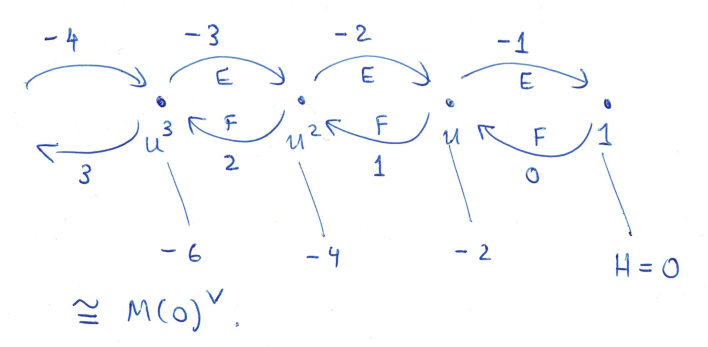
\includegraphics[width=100mm]{D-mod-big-cell.png}
\end{center}

Second let's consider $w = e$. Since the cell is $\{\infty\}$ let's work with the local coordinate $x = 1/u$. Relative to this coordinate we have $X_e = \{0\}$, and $\partial_x$ is a normal vector field. We have $\OO_{*} = \C$, let $\delta$ denote the image of $1$ under the pushforward. Then the pushforward is spanned by $\delta$, $\partial_x \delta$, $\partial_x^2 \delta$, etc. The action of $x$ is determined by the relation $x \delta = 0$. For example this determines that
\[
x(\partial \delta) = \partial(x \delta) - \partial(x) \delta = -\delta
\]




\begin{center}
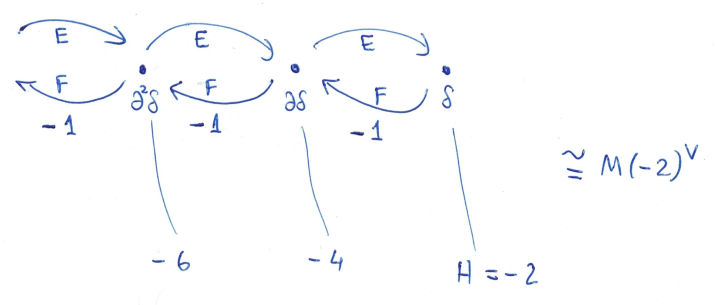
\includegraphics[width=100mm]{D-mod-little-cell.png}
\end{center}

So in fact
\[
\Gamma(X, \M'_e) \cong M(-2)^\vee.
\]

{\color{blue}
\begin{rem}
A bit of a paradox: probably due to a sign error somewhere. Let us consider $\Delta(M(-2))$ and try to confirm the description we just obtained. We present $M(-2)$ as the quotient $U(\g) / U(\g) <E, H+2>$ (quotient of left $U(\g)$-modules). In the big cell with coordinate $u$ we find
\[
\CD / \CD <\partial_u, -2u \partial_u + 2> = \C[u] / (-2u \partial_u + 2)\C[u]
\]

\end{rem}
}


It turns out that $D$-module dual corresponds to contragredient dual in category $\OO$. So if we define $\M_w = \D(\M'_w)$ then $\M_e$ corresponds to $M(-2)$ and $\M_\sigma$ corresponds to $M(0)$.

---------------

Next we need to explain
\begin{align*}
\CL_e &= \M_e, \\
%
\CL_\sigma &= \M_\sigma - \M_e.
\end{align*}
So far there is nothing to explain as the LHS have not been defined. The point is that one defines the LHS in some way (specifically as IC sheaves, which means they are Verdier-self-dual) and a very deep theorem guarantees that they are irreducible in a certain sense (so their global sections correspond to the irreducible $\g$-modules $L_w$).

This requires passing to perverse sheaves via the Riemann-Hilbert correspondence.

The other ingredient is to somehow associate these objects (holomorphic regular $\CD_X$-modules) with elements of the Hecke algebra. In such a way (check details) that $\M_w$ corresponds to the basis element $T_w$, and $\CL_w = \M_w + (lower order)$ has the property that it is invariant under the involution. This ends up proving the Kazhdan-Lusztig conjecture.

The annoying thing is that this requires even more weird theory: Hodge modules, which are a sort of refined hybrid of $\CD$-modules and perverse sheaves.


------------------

The explicit statements about where the Vermas and irreducibles go are as follows:
\begin{thm}
Let $i : X_w \rightarrow G/B$ denote the embedding of a Bruhat cell. There is an isomorphism of $\CD$-modules
\[
\D(M_w^\vee) \cong \int_i \OO_{X_w}.
\]
\end{thm}

\begin{thm}[{\cite[Proposition 12.3.2 (i)]{HTT}}]
Let $i : X_w \rightarrow G/B$ denote the embedding of a Bruhat cell. There is an isomorphism of $\CD$-modules
\[
\D(L_w) \cong i_{!*} \OO_{X_w}.
\]
\end{thm}
First we explain the notation. In general if $f : X \rightarrow Y$ and $\CM$ is a $\CD_X$-module, then there exists a canonical morphism
\[
\int_{f!} \CM \rightarrow \int_f \CM
\]
and we denote its image by $f_{!*} \CM$. This $\CD_Y$-module is called the ``minimal extension'' of $\CM$ relative to $f$.

We fix notation as follows: $U = X_\sigma = \bbP^1 \backslash \{\infty\}$ and $V = \bbP^1 \backslash \{0\}$, with inclusions
\[
j : U \rightarrow \bbP^1 \leftarrow \{\infty\} : i.
\]

{\color{blue}First compute $\int_j \OO_U$ using the more standard triangle.}


If $\CM$ is a left $\CD$-module, then we may consider
\[
\Hom_{\CD_X}(\CM, \CD_X).
\]
We prefer to consider this operation only for relatively ``small'' $\CD$-modules -- we should like them to be coherent as $\OO_X$-modules at least. Intuitively it is like taking the dual of a vector space, if the dimension is infinite then the dimension of the dual is very much larger. The result of this operation is now a right $\CD_X$-module, so we convert it back (and throw in a shift for good measure) defining
\[
\bbD\CM = \Hom_{\CD_X}(\CM, \CD_X) \otimes_{\OO_X} \omega_X^{\otimes -1} [\dim_X].
\]
This operation sends the category (bounded complexes of) coherent $\CD$-modules into itself, and $\bbD^2 = \Id$ {\cite[Proposition 2.6.5]{HTT}}.
\begin{table}[h!]
\centering
\begin{tabular}{ |c|c| }
\hline
Sheaves & $\CD$-modules \\
\hline
$f_*$ & $\int_f$ \\
$f^{-1}$ & $f^\star = \bbD_X \circ f^\dagger \circ \bbD_Y$ \\
$f_!$ & $\int_{f!} = \bbD_Y \circ \int_f \circ \bbD_X$ \\
$f^!$ & $f^\dagger = f^*[\dim_X-\dim_Y]$ \\
$\bbD$ & $\bbD$ \\
\hline
\end{tabular}
\caption{Matching between image functors for plain sheaves and $\CD$-modules}
\label{table:6-func}
\end{table}



The following is {\cite[Theorem 1.7.1]{HTT}}.
\begin{thm}
Let $Z \subset X$ be a closed subset, assume $Z$ is smooth as a variety. Let $i : Z \rightarrow X$ denote the inclusion, and $j : U \rightarrow X$ the inclusion of the complement. Then there exists a distinguished triangle
\[
\int_{i} i^\dagger \CM \rightarrow \CM \rightarrow \int_{j} j^\dagger \CM \xrightarrow{+1}
\]
\end{thm}
If we use plain sheaf notation of Table \ref{table:6-func}, then the distinguished triangle of the theorem above becomes
\begin{align}\label{eq:main.triangle}
i_! i^! \CM \rightarrow \CM \rightarrow j_* j^* \CM \xrightarrow{+1}.
\end{align}
According to {\cite[p. 19]{Jeffs}} and to {\cite[p. 18]{Williamson-illustrated}}, there is another distinguished triangle:
\[
j_! j^! \CM \rightarrow \CM \rightarrow i_* i^* \CM \xrightarrow{+1}
\]
referred to as the triangle ``Verdier dual'' to \eqref{eq:main.triangle}. Let's derive it. According to {\cite[p. 18]{Jeffs}} {\color{blue}This should be somewhere in HTT, just have to find it.} we have $\int_i = \int_{i!}$ for a closed inclusion, and $j^\star = j^\dagger$ for an open inclusion.

Opening up the definitions here gives
\[
\bbD_X i_* \bbD_Z i^! \CM \rightarrow \CM \rightarrow j_* \bbD_U j^! \bbD_X \CM \xrightarrow{+1}
\]
Now let's apply this triangle not to $\CM$ but to $\bbD(\CM)$, and let's also post-compose everything with $\bbD$. The post-composition reverses arrows. We get
\[
 \xleftarrow{+1} i_* \bbD_Z i^! \bbD_X \CM \leftarrow \bbD_X^2 \CM \leftarrow \bbD_X j_* \bbD_U j^! \CM.
\]
A potentially confusing detail: the left-most arrow still has degree $+1$ because the operation $\Hom_{\CD}(-, \CD)$ is understood to send the term in degree $+k$ to degree $-k$ in general. Using the definitions of $i_*$ and $j^!$ again, and $\bbD_X^2 = \Id$, we have
\[
j_! j^! \CM \rightarrow \CM \rightarrow i_* i^* \CM \xrightarrow{+1}.
\]
as required.


Anyway, to compute $\int_j \OO_U$ we use the standard triangle
\[
\int_{i} i^\dagger \CM \rightarrow \CM \rightarrow \int_{j} j^\dagger \CM \xrightarrow{+1}
\]
with $\CM = \OO_{\bbP^1}$. The rightmost term is precisely $\int_j \OO_U$. Now $i^\dagger \OO_{\bbP^1}$ is the $\OO$-module pullback with a homological shift. More precisely it is $\underline\C[-1]$ (i.e., concentrated in homological degree $1$). On $U$ nothing much is happening: we have $\int_j\OO_U(U) = \OO_{\bbP^1}(U)$. On $V$ things are more interesting. Thus the LES is telling us
\begin{align*}
\xymatrix{
\C[\partial_x] \ar@{->}[r] & 0 & \\
%
0 \ar@{->}[r] & \CD / \CD \cdot \partial_x \ar@{->}[r] & ? \ar@{->}[ull] \\
}
\end{align*}
From this we infer
\begin{align}\label{eq:intj}
[\int_{j}\OO_U](V) = \CD / \CD \cdot \partial_x x.
\end{align}


To compute $\int_{j!} \OO_U$ we will use the triangle
\[
\int_{j!} j^! \CM \rightarrow \CM \rightarrow \int_i i^* \CM \xrightarrow{+1}
\]
We take $\CM = \OO_{\bbP^1}$. It is a fact that
\[
j^! \OO_{\bbP^1} = j^* \OO_{\bbP^1} = \OO_U,
\]
so the leftmost term is just what we are computing. Now we proceed by computing on $U$ and on $V$. Firstly on $U$ nothing much happens, we have
\[
[\int_{j!}\OO_U](U) = \OO_{\bbP^1}(U) = \C[u].
\]
On $V$ things are a little more interesting. We claim that
\begin{align}\label{eq:intj!}
[\int_{j!}\OO_U](V) = \CD / \CD \cdot x \partial_x
\end{align}
(where $D = \C[x, \partial_x]$). First we note that $\CM(V) = \OO_{\bbP^1}(V) = \CD / \CD \cdot \partial_x$. Next we recall that $i^* \CM$ is the $\OO$-module pullback as a sheaf, so $i^* \CM = \C$ on the point. {\color{red}Now a confusing point: the pullback $i^\dagger \OO$ would be $\C[-1]$ because of the definition, i.e., concentrated in degree $+1$. But I think the triangle I am using is Verdier dual to the usual one, and $i^*$ is supposed to mean Verdier dual to $i^\dagger$, which in this case just moves $\C$ to degree $-1$.} Now the pushforward is polynomials in $\partial_x$, concentrated in homological degree $-1$. Staring at the LES now
\begin{align*}
\xymatrix{
? \ar@{->}[r] & \CD / \CD \cdot \partial_x \ar@{->}[r] & 0 \\
%
 & 0 \ar@{->}[r] & \C[\partial_x] \ar@{->}[ull] \\
}
\end{align*}
we infer \eqref{eq:intj!}. The map in is just $\partial_x \mapsto \partial_x$ and the map out is the quotient.

So $\int_{j!} \OO_U \rightarrow \int_j \OO_U$ is (1) on $U$ it is the identity map, (2) on $V$ it is the map
\[
\CD / \CD \cdot x \partial_x \rightarrow \CD / \CD \cdot \partial_x x.
\]
The picture is as follows




\begin{figure}[htp]
\begin{center}
\begin{tikzpicture}[scale=1.5]
% Left part:
% dots
\node (1) at (-4, 0) {$\bullet$};
\node (x) at (-3, 1) {$\bullet$};
\node (x2) at (-2, 2) {$\bullet$};
\node (y) at (-3, -1) {$\bullet$};
\node (y2) at (-2, -2) {$\bullet$};
% labels
\node at (-4.3, 0) {1};
\node at (-3.3, 1.3) {$\partial$};
\node at (-2.3, 2.3) {$\partial^2$};
\node at (-3.3, -1.3) {$x$};
\node at (-2.3, -2.3) {$x^2$};
% arrows
\draw[->] (1) to[bend left] node[midway, left] {$\partial$} (x);
\draw[->, dotted] (x) to[bend left] node[midway, right] {$x$} (1);
\draw[->] (x) to[bend left] node[midway, left] {$\partial$} (x2);
\draw[->] (x2) to[bend left] node[midway, right] {$x$} (x);
\draw[->] (1) to[bend left] node[midway, right] {$x$} (y);
\draw[->] (y) to[bend left] node[midway, left] {$\partial$} (1);
\draw[->] (y) to[bend left] node[midway, right] {$x$} (y2);
\draw[->] (y2) to[bend left] node[midway, left] {$\partial$} (y);
%
\node[above right] at (-1.8, 2.2) {$\iddots$};
\node[above right] at (-1.8, -2.7) {$\ddots$};
%
% Right part:
% dots
\node (1') at (0, 0) {$\bullet$};
\node (x') at (1, 1) {$\bullet$};
\node (x2') at (2, 2) {$\bullet$};
\node (y') at (1, -1) {$\bullet$};
\node (y2') at (2, -2) {$\bullet$};
% labels
\node at (-0.3, 0) {1};
\node at (0.7, 1.3) {$\partial$};
\node at (1.7, 2.3) {$\partial^2$};
\node at (0.7, -1.3) {$x$};
\node at (1.7, -2.3) {$x^2$};
% arrows
\draw[->] (1') to[bend left] node[midway, left] {$\partial$} (x');
\draw[->] (x') to[bend left] node[midway, right] {$x$} (1');
\draw[->] (x') to[bend left] node[midway, left] {$\partial$} (x2');
\draw[->] (x2') to[bend left] node[midway, right] {$x$} (x');
\draw[->] (1') to[bend left] node[midway, right] {$x$} (y');
\draw[->, dotted] (y') to[bend left] node[midway, left] {$\partial$} (1');
\draw[->] (y') to[bend left] node[midway, right] {$x$} (y2');
\draw[->] (y2') to[bend left] node[midway, left] {$\partial$} (y');
%
\node[above right] at (2.2, 2.2) {$\iddots$};
\node[above right] at (2.2, -2.7) {$\ddots$};
%
% Central arrow
\draw[->] (1) to[out=0, in=180] node[midway, below] {$\varphi$} (y');
\end{tikzpicture}
\end{center}
\caption{The morphism $\varphi : \CD / \CD x \partial \rightarrow \CD / \CD \partial x$}
\label{fig:2}
\end{figure}
%
% \begin{center}
% 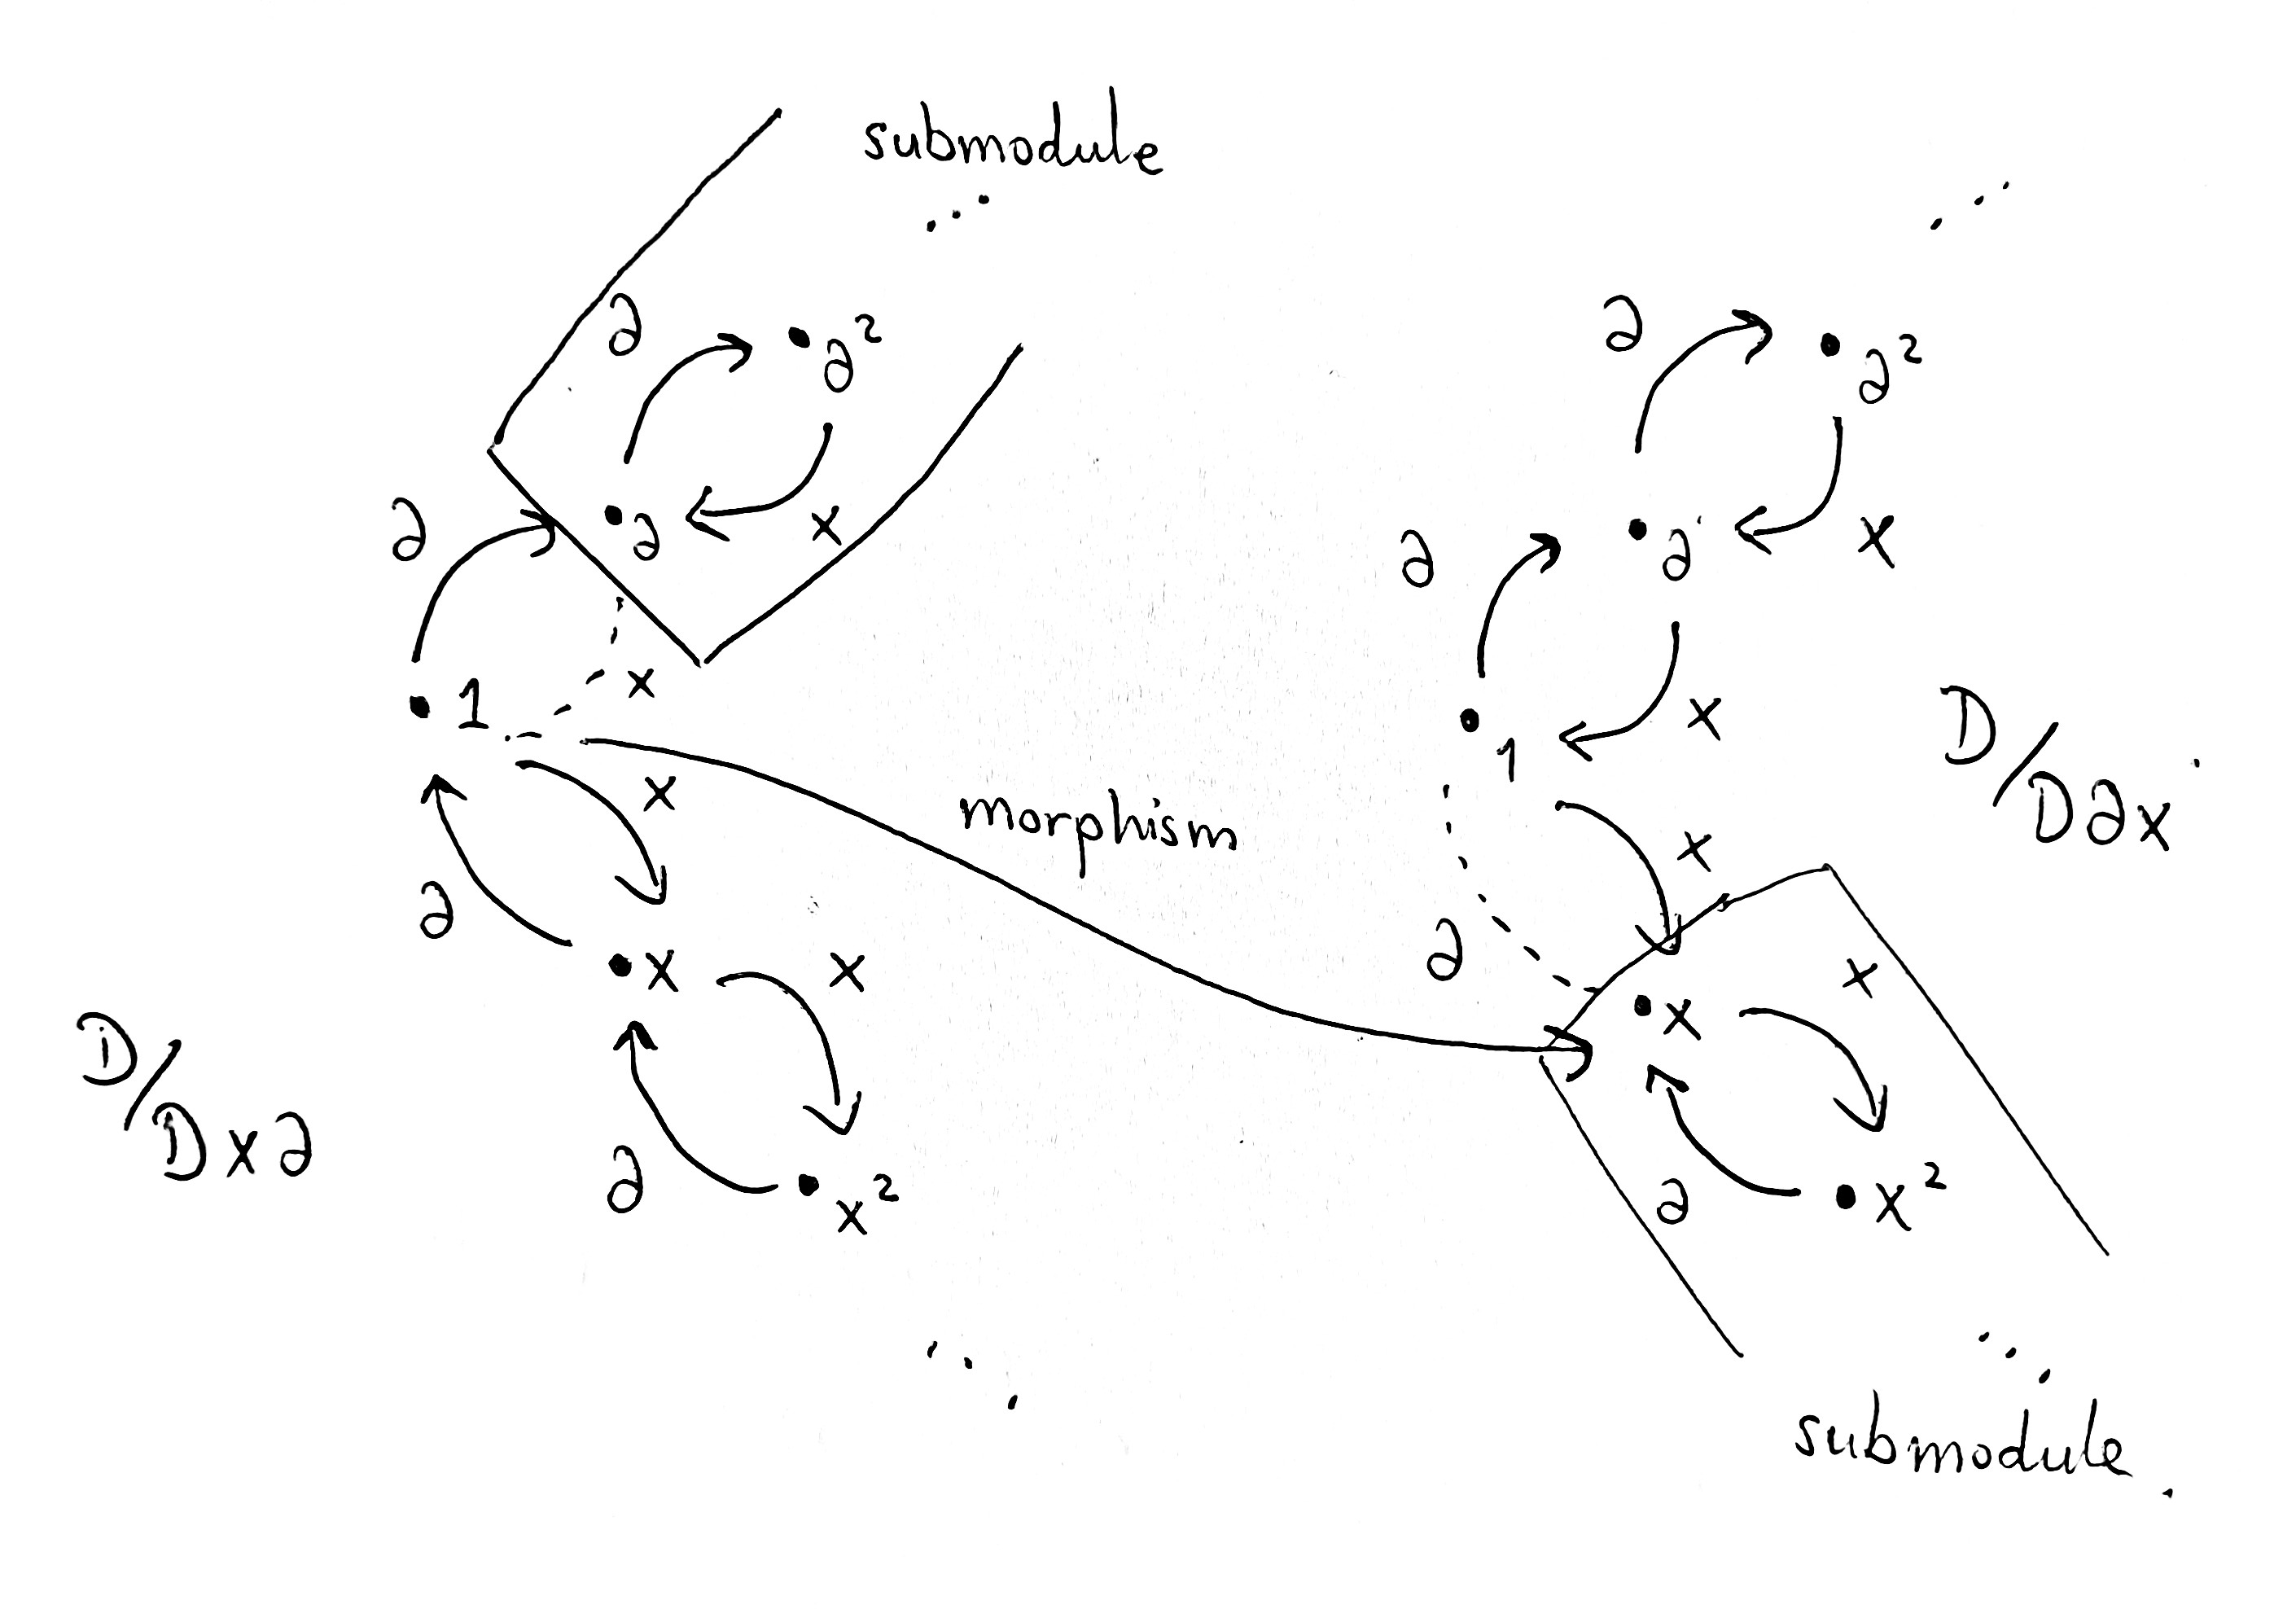
\includegraphics[width=100mm]{intext_1.jpg}
% \end{center}

Inside $\CD / \CD \cdot x \partial_x$ we have the submodule generated by $\partial_x$, the quotient by this submodule is generated by $1$. There is a well-defined morphism of $\CD$-modules killing the submodule and sending $1 \mapsto x$. The image is isomorphic to $\C[x]$ with $x^{k+1}$ playing the role of $x^k$. This might seem peculiar, but consider $\partial_x x =0$ in this module, so indeed $x$ is behaving like $1$.

Anyway we have computed $j_{!*} \OO_U$ to be $\C[u]$ on $u$ and $\C[x]$ on $V$. One can check things match up as expected on the intersection, and indeed
\[
j_{!*} \OO_U \cong \OO_{\bbP^1} = \D(L_\sigma).
\]



\section{Roadmap from here}

\newcommand{\heckat}{\mathbb{H}}

The multiplicities of irreducibles $L_y$ in Vermas $M_w$ (here $w, y \in W$) are computed from a certain weird change-of-basis in the Hecke algebra. To make the connection, the idea roughly is to construct an associative product of $\CD$-modules on $X = G / B$.

The way to do this is to consider the product variety $X \times X$, which carries two left actions of $G$ -- on the left and right factors, respectively. Denote by $\D G$ the diagonal action, i.e.,
\[
g (x_1 B, x_2 B) = (gx_1 B, gx_2 B).
\]
It is easy to check that as sets
\[
X \times X / \D G \cong X / B = B \backslash G / B.
\]
Indeed the action of $G$ on $X$ is transitive, so each $\D G$-orbit contains an element of the form $(eB, gB)$, and now we just note that
\[
(eB, g_1B) \sim (eB, g_2B)
\]
if and only if $g_2 = b g_1$ for some $b \in B$.


It follows that we can write
\[
X \times X = \bigcup_{w \in W} Z_w
\]
where the $Z_w = \D G (eB, n_w B)$ are $\D G$-orbits, similarly to how we wrote
\[
X = \bigcup_{w \in W} X_w
\]
where the $X_w$ are $B$-orbits.

It is now possible to introduce a product on $D$-modules. It is called the convolution product, and is actually an instance of quite a general construction. We consider the following pair of morphisms:
\begin{align*}
\xymatrix{
& (a, b, c) \ar@{|->}[dl] & X^3 \ar@{->}[dl]_{p_{13}} \ar@{->}[dr]^{r} & (a, b, c) \ar@{->}[dr] \\
%
(a, c) & X^2 & & X^2 \times X^2 & (a, b, b, c) \\
}
\end{align*}
Now given $\CD$-modules $M$ and $N$ on $X^2$, we define
\[
[M] * [N] = \sum_{k \in \Z} (-1)^k H^k \int_{p_{13}} r^*(M \boxtimes N).
\]
If $M$ and $N$ are $\D G$-equivariant, then so is their product.



Then we consider coherent $\D G$-equivariant $\CD$-modules on $X \times X$. Call this category $\heckat$.

Turns out {\cite[Proposition 13.1.3]{HTT}} and  $K(\heckat) \cong \C[W]$ with isomorphism
\[
[\bbD \int_{i_w}\OO_{Z_w}] \mapsto (-1)^{\ell(w)} T_w.
\]
One finds that the irreducibles go to $(-1)^{\ell(w)} C_w|_{q=1}$. Now these elements lie in $\C[W]$ but their definition requires the passage to the Hecke algebra (they are characterised by being invariant under some involution).

So it is necessary to somehow put $q$ into the structure of our category $\heckat$. Then it will turn out, roughly, that the involution corresponds to Verdier duality, and the invariance of the $\CL_w$ comes from a deep result called the decomposition theorem.



\begin{defn}
Let $A = \Z[q^{1/2}, q^{-1/2}]$. The Hecke algebra $H$ is quotient of the free associative $A$-algebra with generators $T_s$ for $s = 1, \ldots, \ell$ by the relations
\[
(T_i T_j)^{m_{ij}} = (T_j T_i)^{m_{ij}},
\]
and
\[
T_s^2 = (q-1)T_s + q T_e.
\]
\end{defn}
It turns out that $H$ is a free $A$-module of rank equal to the cardinality $|W|$ of the Weyl group $W$, and a basis of $H$ is given by
\[
T_w = T_{s_{i_1}} T_{s_{i_2}} \cdots T_{s_{i_\ell}}, \qquad w \in W
\]
where $w = s_{i_1}s_{i_2}\cdots s_{i_\ell}$ is a reduced expression (Remarkably, different reduced expressions for $w$ yield the same element $T_w$).

There is an involution, denoted $X \mapsto \ov{X}$ on $H$ (as a $\Z$-algebra) which interchanges $q^{1/2}$ with $q^{-1/1}$ and $T_w$ with $(T_{w^{-1}})^{-1}$. There is a unique basis $\{ C_{w} \mid w \in W \}$ of $H$ with the property $\ov{C_w} = C_w$ for each $w \in W$, and
\[
C_w = q^{-\ell(w)/2} \sum_{y \leq w} Q_{y, w}(q^{1/2}) T_y,
\]
for some polynomials $Q_{y, w}(t)$ where $Q_{w, w}(t) = 1$ and $\deg(Q_{y, w}) \leq \ell(w) - \ell(y) - 1$. This is reasonably easy to prove, actually.

It turns out, furthermore, that $Q_{y, w}(q^{1/2}) = P_{y, w}(q)$ (i.e., only even powers of $t$ appear in $Q_{y, w}(t)$).

Then the Kazhdan-Lusztig conjecture (now theorem) says:
\begin{thm}
At the level of characters
\[
[L_{w}] = \sum_{x \leq w} (-1)^{\ell(w)-\ell(x)} {P}_{x, w}(1) [M_x].
\]
\end{thm}
Here are some examples, which I have taken from the nice review paper \cite{Riche}. For example for $G = SL_3$ the algebra $H$ has a basis
\[
T_e, \quad T_1, \quad T_2, \quad T_{12}, \quad T_{21}, \quad \text{and} \quad T_\circ,
\]
and we have
\begin{align*}
C_e &= T_e \\
%
C_1 &= q^{-1/2}(T_1 + 1), \\
%
C_2 &= q^{-1/2}(T_2 + 1), \\
%
C_{12} &= q^{-1}(T_{12} + T_1 + T_2 + 1), \\
%
C_{21} &= q^{-1}(T_{21} + T_1 + T_2 + 1), \\
%
C_\circ &= q^{-3/2}(T_\circ + T_{12} + T_{21} + T_1 + T_2 + 1).
\end{align*}
Examining the expression for $C_{\circ}$, we see that the Weyl-Kac character formula is confirmed. In fact this particular expression is always particularly simple, i.e., $P_{x, w_\circ}(q) = 1$ for all $x$. For larger groups, the polynomials become more complicated. Already in the case of $G = SL_4$ one has
\begin{align*}
C_{2132} = {} & q^{-2} ( T_{2132} + T_{213} + T_{212} + T_{232} + T_{132} + \\
%
 &+ T_{21} + T_{12} + T_{13} + T_{23} + T_1 + T_3 + (1+q)T_2 + (1+q)T_e ).
\end{align*}


The proof revolves around the geometry of $X = G / B$, the Bruhat cells $X_w = B w B / B \subset X$ and the Schubert varieties $\ov{X}_w$. One has $X_x \subset \ov{X}_w$ if and only if $x \leq w$.

Poincaré polynomial of $\ov{X}_w$:
\[
P_w(q) = \sum_{i \in \Z} \dim H^{2i}(\ov{X}_w) q^i
\]

The Kazhdan-Lusztig polynomials are Poincaré polynomials of intersection homology groups
\[
P_{x, w}(q) = \sum_{i \in \Z} \dim IH_x^{2i}(\ov{X}_w) q^i.
\]
There is also $IH(\ov{X}_w)$ (no subscript) around
\[
\sum_{i \in \Z} \dim IH^{2i}(\ov{X}_w) q^i = \sum_{x \leq w} q^{\ell(x)} {P}_{x, w}(q).
\]


Sometimes Poincaré duality fails for $H$, but is always maintained by $IH$


(A) Let $D = D_X = \Gamma(X, \CD_X)$, and let $U_0 = U(\g) / \ker(\chi_0)$. Prove that $D_X \cong U_0$.

(B) Let $\CC'$ be the category of all $D$-modules, and $\CC$ be the category of $\OO$-quasicoherent $\CD$-modules on $X$. There are functors of localisation and global sections. Highly nontrivial theorem: these are equivalences of categories.


There is the subcategory $\CC_0'$ of $U(\frakb)$-finite finitely generated modules. This corresponds to $\CC_0 \subset \CC$ of $\CD$-modules (1) killed by an ideal of finite codimension in $U(\frakb)$ and (2) with a $U(\frakb)$-stable good filtration.

Another important theorem: all objects of $\CC_0$ are regular and holonomic.

(C) The Riemann-Hilbert correspondence {\cite[Theorem 7.2.2]{HTT}} says that if $X$ is a smooth algebraic variety, then
\[
DR : D^b_{rh}(D_X) \rightarrow D^b_c(X)
\]
is a equivalence, and {\cite[Theorem 7.2.5]{HTT}} The image of $\CD_X-mod_{rh}$ under $DR$ is the abelian category of perverse sheaves.

By the way, the definition of $DR_X$ appears on p. 103, and is basically
\[
DR_X(M^\bullet) = \Om_X \otimes^L_{D_X} M^\bullet.
\]
This definition makes it look like one can work algebraically. But it's very important, actually, to first analytify. I have very little intuition for why it's so vital. But a remark is that the solution functor $\Hom_{D_X}(-, \OO_X)$ is quite similar, in that it coincides with $\otimes$ up to shift or something. And it's quite clear that the solution functor gives drastically different results if we work analytically or algebraically, as the example the exponential function illustrates.

(The definition of the RHS involves the Bruhat stratification, it must enter the definition of the LHS too).

So Vermas $M_w$ and simples $L_w$ go to specific perverse sheaves. The Verma modules are each sent to a constructible sheaf supported on a single Bruhat cell. The simple objects are sent to ``intersection cohomology'' sheaves.

%The description in Humphreys ends here. Need to take up the story with HTT.




\section{The Hecke algebra}


The proof of the Borel-Weil theorem suggests that the set $B \backslash G / B$ is important. In fact functions on this set form a remarkable algebra called the Hecke algebra.


Let $G$ be a finite group and $B$ a subgroup of $G$. For the development of this course, the groups $G$ and $B$ will be the $\F_p$-points of a simple algebraic group $G$ and $B$ a Borel subgroup. But the general construction works in general.

If $S$ is any set, we denote by $C(S)$ the vector space of functions $f : S \rightarrow \C$ with pointwise addition.

The convolution $* : C(G) \times C(G) \rightarrow C(G)$ is defined by
\[
[f_1 * f_2](g) = \frac{1}{|G|} \sum_{x \in G} f_1(x) f_2(x^{-1}g).
\]

Obviously $C(G / B)$ is naturally identified with the subset
\[
\{f : G \rightarrow \C | \text{$f(gb) = f(g)$ for all $g \in G$, $b \in B$}\},
\]
of $C(G)$. Then
\[
[f_1 * f_2](gb) = \frac{1}{|G|} \sum_{x \in G} f_1(x) f_2(x^{-1}gb),
\]
and so $f_1 * f_2 \in C(G/B)$ whenever $f_2 \in C(G/B)$. So we have
\[
*: C(G) \times C(G/B) \rightarrow C(G/B).
\]
In a similar way we have
\[
*: C(B \backslash G) \times C(G) \rightarrow C(B \backslash G).
\]
The second one is the same argument, but with a change of summation variable in the middle.

%On the other hand if
%\[
%f_1, f_2 \in C(B \backslash G) = \{f : G \rightarrow \C | \text{$f(bg) = f(g)$ for all $g \in G$, $b \in B$}\}
%\]
%then
%\begin{align*}
%[f_1 * f_2](bg) = \frac{1}{|G|} \sum_{x \in G} f_1(x) f_2(x^{-1}bg) \\
%%
%= \frac{1}{|G|} \sum_{y \in G} f_1(by) f_2(y^{-1}g) = [f_1 * f_2](g),
%\end{align*}
%where I substituted $y^{-1} = x^{-1} b$, so $x = by$.

The Hecke algebra associated to $(G, B)$ is now defined to be $H(G, B) := C(B \backslash G / B)$ with the convolution product, which it is indeed closed under.

If $G$ is the $\mathbb{F}_q$-points of a simple/semisimple/reductive algebraic group and $B \subseteq G$ the corresponding Borel then there is a theorem that $B \backslash G / B$ is in bijection with $W$ the Weyl group (Bruhat decomposition?).

This Hecke algebra can be explicitly described (first studied by Iwahori?) by generators (the $T_s$ associated to generating reflections $s \in W$) and relations, which are like
\[
(T_s + 1)(T_s + q) = 0.
\]

Comparing with the usual answer for $SL_2(\Z_2)$ checks out except the normalisation is a bit off. Probably the standard normalisation is to divide by $|B|$ rather than $|G|$.

More symmetrically
\[
[f_1 * f_2](g) = \sum_{xy = g} f_1(x) f_2(y).
\]
The double coset of $g$ only depends on $Bx$ and $yB$. So we can figure out the convolution of two indicator functions (on the double cosets $Bw_1B$ and $Bw_2B$ say) by writing $Bw_1B = \cup_i Ba^{(1)}_i$ and $Bw_2B = \cup_j a^{(2)}_jB$. The we look at the products $a^{(1)}_i a^{(2)}_j$ and count how many lie in each double coset, these numbers give the coefficients of the indicator functions that occur in the product of our two double cosets.

Though if you think about it, the convolution $\delta_B * \delta_B$ is now $|B| \delta_B$ because each $x \in B$ contributes $1$ in the sum and they all contribute to the double coset $B$. So indeed the correct normalisation is to divide by $|B|$.

















\section{The (weak) BGG resolution}


Let $\g$ be a finite dimensional simple Lie algebra. Recall the Weyl character formula
\begin{align*}
\ch_{L(\La)} = \sum_{w \in W} \varepsilon(w) \ch_{M(w \circ \La)},
\end{align*}
valid whenever $\La \in P_+$. Imagine there were a complex $D_\bullet$ in which $D_0 = M(\La)$, $D_1 = \bigoplus_{i=1}^\ell M(s_i \circ \La)$ and in general $D_n = \bigoplus_{\ell(w)=n} M(w \circ \La)$, so that
\begin{align*}
H_i(D_\bullet) = \begin{dcases}
L(\La) & i=0 \\
0 & i \neq 0
\end{dcases}
\end{align*}
That would be very nice since, because $\varepsilon(w) = (-1)^{ell(w)}$, the Poincaré principle applied to $D_\bullet$ would immediately yield the Weyl character formula.

In fact it is true, and the resolution is called the BGG resolution. We will construct something a little weaker than $D_\bullet$ as described above, instead we will construct a complex $D_\bullet$ for which each $D_n$ carries a filtration
\[
D_n = D_n^{(0)} \supset D_n^{(1)} \supset \ldots \supset D_n^{(N)} = 0,
\]
whose successive quotients are precisely the $M(w \circ \La)$ for $\ell(w)=n$ in some order. Since a filtered module and its associated graded always have the same character, the existence of this weak BGG resolution is still sufficient to prove the Weyl character formula.

The material in this section is taken quite directly from {\cite[Sections 6.1-6.4]{humbgg}}.

-----------------------


We will construct a first approximation to the desired complex by imitating the Chevalley-Eilenberg complex of usual Lie algebra homology. Instead of
\[
V_n = U(\g) \otimes_{\C} \wedge^n \g,
\]
we take
\[
D_n = U(\g) \otimes_{U(\fb)} \wedge^n(\g/\fb).
\]
The differential looks similar, in detail it will be
\begin{align*}
d(u \otimes \xi_1 \wedge \ldots \wedge \xi_n) = {} & \sum_{i=1}^{n} (-1)^{i+1} (u z_i) \otimes \xi_1 \wedge \ldots \wedge \what\xi_i \wedge \ldots \wedge \xi_n \\
&+ \sum_{i < j} (-1)^{i+j} u \otimes \ov{{[\xi_i, \xi_j]}} \wedge \xi_1 \wedge \ldots \wedge \what\xi_i \wedge \ldots \wedge \what\xi_j \wedge \ldots \wedge \xi_n.
\end{align*}
Here $\xi_i \in \g/\fb$ and $z_i$ means any representative in $\g$ of $\xi_i$. Then the overline means to project back to $\g/\fb$. In addition to checking that $d \circ d = 0$ we have to prove that $d$ is actually well-defined. For this it is essential that the tensor product is over $U(\fb)$, which we use to pass elements of $\fb$ back and forth across it.

Proving that $D_\bullet$ is exact, in general, requires a spectral sequence argument like in the usual case. If we happen to be in a situation where $\g = \fb \oplus \n_-$ a splitting of vector spaces in which $\fb$ and $\n_-$ are both subalgebras... then we can cheat and prove the result very easily.

The idea is this: by the PBW theorem we have
\[
U(\g) \cong U(\n_-) \otimes_\C U(\fb),
\]
we also have $\g / \fb \cong \n_-$. So we have vector space isomorphisms
\[
U(\g) \otimes_{U(\fb)} \wedge^n(\g/\fb) \cong U(\n_-) \otimes_\C \wedge^n(\n_-),
\]
choose all coset representatives to actually lie in $\n$. Then the differential coincides exactly with the usual Chevalley-Eilenberg differential for $\n_-$. So we have an isomorphism of complexes at the level of vector spaces, which yields exactness.



\begin{rem}
One might ask, given that $D_\bullet(\g, \fb) \cong V_\bullet(\n_-)$, what advantage is gained by introducing $D_\bullet(\g, \fb)$? One way to say it would be to observe that $V_\bullet(\n_-)$ acquires a $\g$-module structure compatible with the differentials. If we did not know the isomorphism to $D_\bullet(\g, \fb)$ then this would not be at all easy to see. Indeed the action of $x \in \g$ would involve multiplying by $x$ from the left, commuting it through, writing it as $x=n+b$, letting $b$ pass to the exterior algebra factors.
\end{rem}



-----------------------

Sumarising, we have
\begin{align*}
H_i(D_\bullet) = \begin{dcases}
\C & i=0 \\
0 & i \neq 0
\end{dcases}
\end{align*}
a resolution of the trivial $\g$-module $\C$. We would like to check that the $D_n$ are filtered by Verma modules. This follows from the general Lemma \ref{lem:Verma.filtration}.

This lemma also tells which Verma factors appear in each $D_n$ and with what multiplicities. A little thought reveals that $D_n$ is much larger than $\{w \in W \mid \ell(w) = n\}$. Indeed if that were the case, we would have a total of $\# W$ Vermas, but actually if $m = \dim(\g/\fb)$ we have $\dim \wedge^\bullet(\g/\fb) = 2^m$ and so we have $2^m$ Vermas, which is much more.

Luckily $D_\bullet$ splits into many subcomplexes, only one of which has a nonzero morphism to $\C$, we need to single out this summand, and we will see that it has the desired number of Verma factors.

{\color{red}
Next we are going to prove a key property of the weights occuring in the $\fb$-module $\wedge^*(\g/\fb)$. First we need some lemmas.

\begin{defn}
For a subset $\Sigma \subset \D_+$ we will denote by $|\Sigma|$ the sum of all the elements in $\Sigma$.
\end{defn}
So for example $|\D_+| = 2\rho$.

\begin{defn}
For $w \in W$ we will denote
\[
\Pi_w = \D_+ \cap w(\D_-).
\]
\end{defn}
The first lemma is this:
\begin{lemma}\label{lem:w.0}
\[
w \circ 0 = -|\Pi_w|.
\]
\end{lemma}


We will also require two other lemmas which we have already proved. Namely
\begin{lemma}
For each simple root $\al_i$ we have
\begin{align*}
s_i(\D_+ \backslash \{\al_i\}) = \D_+ \backslash \{\al_i\}.
\end{align*}
\end{lemma}
And
\begin{lemma}
Let $w \in W$ of length $\ell(w) = k$. Then there exists $i$ such that $r_i w$ has length $k-1$. Furthermore
\[
w^{-1}(\al_i) \in \D_- \qquad \text{and} \qquad (r_iw)^{-1}(\al_i) \in \D_+.
\]
\end{lemma}
(Although not identical, convince yourself that this follows from Lemma \ref{lem:reduced.expression.lemma}.)
}


\begin{prop}
For each $w \in W$ the weight $w \circ 0$ appears among the weights of $\wedge^*(\g/\fb)$ with multiplicity $1$.
\end{prop}

\begin{proof}
We write $m = \dim(\g/\fb) = \# \D_+$. The dimension of $\wedge^*(\g/\fb)$ is $2^m$ with a contribution of $1$ from each subset $\Sigma \subset \D_+$. The nonzero basis vector contributed by $\Sigma$ is
\[
 \pm e_{-\al_1} \wedge \cdots \wedge e_{-\al_n} \quad \text{where} \quad \Sigma = \{\al_1, \ldots \al_n\}.
\]

Suppose $\mu = w \circ 0$, then by Lemma \ref{lem:w.0} we have $\mu = -|\Pi_w|$. This interpretation allows us to deduce the multiplicity $1$ property from the following lemma.
\end{proof}

\begin{lemma}
Let $w \in W$ and $\Sigma \subset \D_+$. If $|\Sigma| = |\Pi_w|$ then $\Sigma = \Pi_w$.
\end{lemma}


\begin{proof}
The proof is by induction on the length $\ell(w)$. For the base case we note that $\ell(w) = 0$ only for $w=e$, we have $\Pi_e = \emptyset$ and $|\Pi_e| = 0$, and then since all the elements of $\D_+$ are on one side of a hyperplane, clearly $|\Sigma| = 0$ only for $\Sigma = \emptyset = \Pi_e$.

Now we suppose the result has been established for all $w$ of length at most $k$, and choose $w$ of length $\ell(w) = k > 0$. There exists a simple root $\al \in \Pi$ such that
\begin{align*}
\ell(s_\al w) &= k-1 \\
%
w^{-1}(\al) &\in \D_- \\
%
(s_\al w)^{-1}(\al) &\in \D_+.
\end{align*}
Write $w' = s_\al w$. In particular $\al \in \Pi_w$ and $\al \notin \Pi_{w'}$.

Recall that
\begin{align*}
s_\al(\D_+ \backslash \{\al\}) = \D_+ \backslash \{\al\}.
\end{align*}
From this we will deduce that
\begin{align*}
\Pi_w = s_{\al}(\Pi_{w'}) \cup \{\al\}.
\end{align*}
Indeed
\begin{align*}
s_{\al}(\Pi_{w'}) &= s_{\al}(\Delta_+) \cap s_{\al}(w'(\Delta_-)) \\
%
&= ((\Delta_+ \backslash \{\al\}) \cup \{-\al\}) \cap w(\Delta_-) \\
%
&= (\Delta_+ \backslash \{\al\}) \cap w(\Delta_-) \qquad \text{(since $\{-\al\} \cap w(\Delta_-) = \emptyset$)} \\
%
&= \Pi_w \backslash \{\al\}.
\end{align*}


Now suppose that $\Sigma \subset \D_+$ with $|\Sigma| = |\Pi_w|$. Since we have $\al \in \Pi_w$ and $\al \notin \Pi_{w'}$, and we are supposed to be proceding by induction, it seems like a good idea to try to relate $\Pi_{w'}$ with $\Sigma \backslash \{\al\}$.

First suppose $\al \in \Sigma$. Then
\begin{align*}
|\Sigma \backslash \{\al\}| = |\Sigma| - \al = |\Pi_w| - \al = \rho - w(\rho) - \al,
\end{align*}
whence
\begin{align*}
|s_\al(\Sigma \backslash \{\al\})| = s_\al|\Sigma \backslash \{\al\}| = s_\al(\rho - w(\rho) - \al) = \rho - \al - w'(\rho) + \al = \rho - w'(\rho) = |\Pi_{w'}|.
\end{align*}
Hence by induction $s_\al(\Sigma \backslash \{\al\}) = \Pi_{w'}$, and so
\[
\Sigma = s_{\al}(\Pi_{w'}) \cup \{\al\} = \Pi_w
\]
as required.


Next suppose $\al \notin \Sigma$. We shall derive a contradiction, thus completing the proof. Well in this case $\Sigma \subset \D_+ \backslash \{\al\}$, so $s_\al(\Sigma) \subset \D_+ \backslash \{\al\}$ and thus
\[
s_\al(\Sigma) \cup \{\al\} \subset \D_+.
\]
By a similar calculation as above, we have
\begin{align*}
|s_\al(\Sigma) \cup \{\al\}| &= s_\al|\Sigma| + \al = s_\al|\Pi_w| = s_\al(\rho - w(\rho)) + \al \\
%
&= \rho - \al - w'(\rho) + \al = \rho - w'(\rho) = |\Pi_{w'}|.
\end{align*}
By induction $s_\al(\Sigma) \cup \{\al\} = \Pi_{w'}$, but we already know that $\al \notin \Pi_{w'}$, so there is a contradiction and this case (namely $\al \notin \Sigma$) does not occur.

\end{proof}

OK that was pretty exhausting, but we have the conclusion that



\section{The Chevalley restriction theorem}

The material of this section is explained in {\cite[Chapter 10]{HTT}}.

Let $V$ be a vector space over $\C$. We denote by $\C[V]$ the algebra of polynomial functions on $V$. (If we choose a basis of the dual of $V$ then each of these is by definition a linear, hence polynomial, function on $V$ and $\C[V]$ is the unital algebra generated by these.)

Let $K$ be a group and $V$ a $K$-module. Then we have a representation of $K$ on $\C[V]$ by
\[
[g \cdot f](v) = f(g^{-1} \cdot v).
\]
We denote by $\C[V]^K$ the set of $K$-invariant elements, which is a subalgebra.

Suppose $K$ is a finite group now. Then it is possible to show that $\C[V]^K$ is finitely generated.

\begin{thm}[Chevalley restriction theorem]
Let $G$ be a simple complex Lie group with Lie algebra $\g$ and Cartan subalgebra $\h$. Then under the restriction map
\[
\rho : \C[\g] \rightarrow \C[\h],
\]
we have
\[
\rho(\C[\g]^G) = \C[\h]^W.
\]
\end{thm}

\begin{proof}
For definiteness let us write $\sigma$ for the map $\C[\g]^G \rightarrow \C[\h]$. First we show that $\sigma$ is injective.

Let $f \in \ker(\sigma)$, which is to say $f(h) = 0$ for all $h \in \h$. At the same time $f$ is $G$-invariant. So if we can show $\Ad(G) \h \subset \g$ is Zariski dense then we will know that $f = 0$. So consider the action
\begin{align*}
\varphi : G \times \h \rightarrow \g \\
%
(g, h) \mapsto \Ad(g)h
\end{align*}
At a point $p = (e, h)$, the differential $d\varphi_p$ is
\begin{align*}
d\varphi_p(X, h') = h' + [X, h].
\end{align*}
If we choose $h$ so that $\al(h) \neq 0$ for all $\alpha \in \D$ then we see that $d\varphi_p$ is surjective. This implies that the image of $\varphi$ contains an open set in the metric topology, and hence is Zariski dense in $\g$.

Now we show that $\sigma(\C[\g]^G) \subset \C[\h]^W$. We think of $W$ as
\[
W = N_G(H) / H,
\]
The action of $w$ on $\h$ coincides with the adjoint action $\Ad(\wtil{w})$ of any chosen lift $\wtil{w}$ of $w$ to $N_G(H)$. But since the restriction of $\Ad$-invariant functions are $\Ad$-invariant, the inclusion follows immediately.


Finally we show equality $\sigma(\C[\g]^G) = \C[\h]^W$.

Recall $L(\lambda)$ the finite dimensional irreducible r$\g$-module (and $G$-module by exponentiation) of highest weight $\la \in P_+$. Set $f_{\la, m} \in \C[\g]$ defined by
\[
f_{\la, m}(X) = \tr_{L(\la)} X^m.
\]
We claim that $f_{\la, m} \in \C[\g]^G$, which is easy to see because
\[
\tr_{L(\la)} g X g^{-1} =  \tr_{L(\la)} X.
\]
If we can show that $\sigma(f_{\la, m})$ span $\C[\h]^W$ then we will be done.

Now we conisder also the \emph{formal} character of $L(\la)$, namely
\[
\chi_{L(\la)} = \sum_{\mu \in \h^*} \dim(L(\la)_\mu) e^\mu \in \C[P],
\]
where $\C[P]$ denotes the $\C$-algebra $\bigoplus_{\mu \in P} \C e^\mu$ with product $e^\mu \cdot e^{\mu'} = e^{\mu + \mu'}$. Alternatively think of $\C[P]$ as the collection of all functions $f : P \rightarrow \C$ with finite support.

{\color{red}There are two natural products on $\C[P]$ -- considered as set functions $P \rightarrow \C$ -- the pointwise product, which is what is implicit when we speak of the algebra $\C[V]$ above, and the convolution product.}

The action of $W$ on $\h$ induces an action on $\h^*$, under which $P$ is invariant. So we can speak of $\C[P]^W$. We claim that $\C[P]^W$ is spanned by $\chi_{L(\la)}$ for $\la \in P_+$. Note first that each $W$-orbit in $P$ meets $P_+$. Now let $f \in \C[P]^W$ and cosider its support, let $\mu \in P$ be the highest weight in the support of $f$. Proceed by reverse induction on height now, the weight $\mu$ lies in $P_+$, and we subtract
\[
f - f_\mu \chi_{L(\mu)}
\]
to get another $W$-invariant function of strictly lower height. That dispenses with the claim.

Next we consider
\begin{align*}
\C[P] \rightarrow \C[[\h]] \rightarrow \C[\h]_m
\end{align*}
given by
\[
e^{\la} \mapsto \sum \la^j / j!, \quad \text{and} \quad \text{(extract homogeneous degree $m$ component)}.
\]
We prove $\C[P]^W \rightarrow \C[\h]_m^W$ is surjective, then we will be done. First note that $\C[P] \rightarrow \C[\h]_m$ is surjective. Why is this? Well we could grab a basis $\{\varpi_1, \ldots, \varpi_\ell\}$ of $P$, on which the map gives $e^{\varpi_i} \mapsto \varpi_i^m$. These images do not span, but if we also take $e^{\varpi_1 + \varpi_2}$, for instance, then it goes to $(\varpi_1+\varpi_2)^m$, and together we get all the degree $m$ monomials as linear combinations. So grab $f \in \C[\h]_m^W$, choose a preimage in $\wtil{f} \in \C[P]$, do an averaging
\[
\what{f} = \frac{1}{\# W} \sum_{w \in W} w \wtil{f} \in \C[P]^W
\]
and observe that $\what{f} \mapsto f$.
\end{proof}

\begin{prop}
Let $X \in \g$, then the intersection of $\Ad(G) \cdot X$ with $\h$ is either empty or a single $W$-orbit.
\end{prop}

\begin{proof}
Since for every $w \in W$ the action of $w$ on $\h$ is given by the action of some $\wtil w \in G$, the intersection (if nonempty) must be a union of $W$-orbits. Now let $h_1, h_2 \in \h$ in the same $G$-orbit, we wish to show that they are in the same $W$-orbit.

We are supposed to use $\rho(\C[\g]^G) = \C[\h]^W$ somehow. To do so it helps to think of the points $h_1, h_2$ algebraically: they correspond to two homomorphisms $\ev_{h_1}$, $\ev_{h_2}$ of $\C$-algebras $\C[\g] \rightarrow \C$ (namely, evaluation of a function at the point). By composing with $\sigma$ they give two homomorphisms $\C[\g] \rightarrow \C$ (this just corresponds to the )
\end{proof}


Let $Z(\g)$ denote the centre of $U(\g)$, i.e.,
\[
Z(\g) = \{z \in U(\g) \mid \text{$zu = uz$ for all $u \in U(\g)$}\}.
\]
\begin{lemma}\label{lem:verma.has.char}
Let $M(\La)$ be a Verma module for $\g$. Every $z \in Z(\g)$ acts in $M(\La)$ as some constant.
\end{lemma}

\begin{exer}
Prove the lemma.
\end{exer}
% Step 1: $z$ commutes with every $h \in \h$ so it maps the highest weight vector to some multiple of itself.

% Step 2: Actually that's it.

Let $M$ be a $\g$-module, and suppose each $z \in Z(\g)$ acts in $M$ by a constant, which we denote $\chi(z)$. Then $\chi : Z(\g) \rightarrow M$ is a homomorphism, which we call the central character of $M$.





The Harish-Chandra theorem.
\begin{thm}
Suppose $L(\la)$ is a composition factor of $M(\La)$. Then $\la \leq \La$ and $\la = w \circ \La$ for some $w \in W$.
\end{thm}

\begin{proof}
From Lemma \ref{lem:verma.has.char} we know that $M(\La)$ has some central character $\chi = \chi_\La$. Every submodule and quotient (and therefore $L(\la)$) has the same central character. That is,
\[
\chi_\la = \chi_\La.
\]

\end{proof}



\section{The Nilpotent cone}


Theorem of Kostant is 3.2.5 in the book Chriss-Ginzburg.

This theorem is needed later in the proof that $G/B$ is $D$-affine.





\section{Pushforward with compact support}

...

{\color{blue} I see this used in the material on constructible sheaves, but not really for $\CD$-modules. Indeed for $\CD$-modules I see $f^*$ and $f^!$, with the latter being defined as a homological shift of $f^*$ (HTT p. 33 and Bernstein p. 5).

On the other Verdier duality is an essential ingredient of the perverse sheaves story, and it totally uses $f_!$ and its left adjoint. So I guess I need to cover this stuff.

}


Let $f : X \rightarrow Y$ be a continuous map of topological spaces. By definition the proper direct image $f_!\CF$ is defined by
\[
f_!\CF(V) = \{ s \in \CF(f^{-1}(V)) \mid \text{The restriction $f|_{\supp(s)} : \supp(s) \rightarrow V$ is a proper map} \}
\]
By its definition we have an injective morphism of sheaves $f_!\CF \rightarrow f_*\CF$.

The support of a section of a sheaf is the set of points at which the germ is nonzero. The support of a sheaf is a different notion, it is the set of points at which the stalk is nonzero. The support of a section of any sheaf is always a closed set. Not necessarily so for the support of a sheaf. [Hartshorne, II. Exercise 1.14, p. 67]

One can find the definition of ``proper morphism'' of schemes in Hartshorne, p. 100. But here we are talking about topological spaces in general. The definition is
\begin{defn}
A continuous function $f : X \rightarrow Y$ is proper if for all $K \subset Y$ compact, the imverse image $f^{-1}(K)$ is compact.
\end{defn}
%It's probably instructive to prove that $f_!\CF$ is a sheaf, though I have never done this.

If $f$ is a proper map then evidently the preimage of every point is compact. Perhaps this is a sensible intuition for the notion of proper.


We reserve the symbol $\Gamma_c(X, -)$ for $\pi_!(-)$ the compactly supported pushforward along the surjection $\pi : X \rightarrow *$ to a point.


{\color{red}Recovering Poincare from Verdier is HTT Example C.2.16}





\section{The derived category}

This section based on {\cite[Chapter 2]{Huybrechts}}.

Let $\CA$ be an abelian category. A complex of objects of $\CA$ is a collection of objects and morphisms as follows
\[
\cdots \rightarrow A^{-1} \rightarrow A^0 \rightarrow A^1 \rightarrow \cdots,
\]
in which $d \circ d = 0$. A morphism $A \rightarrow B$ of complexes is a set of $f^i : A^i \rightarrow B^i$ such that all the obvious squares commute. There is a category, denoted $Kom(\CA)$, whose objects are complexes and morphisms are morphisms of complexes.

This category is again abelian (Proposition 2.3). It comes with an operation called ``shift'' or ``suspension'': $A \mapsto A[1]$ defined by $A[1]^i = A^{i+1}$, and $d[1]^i = -d^{i+1}$. Think of $A[1]$ as ``$A$ shifted one step left''.



Given a complex $A$, one can form cohomology
\[
H^i(A) = \frac{\ker(d : A^i \rightarrow A^{i+1})}{\im(d : A^{i-1} \rightarrow A^i)},
\]
thus obtaining an infinite sequence of elements of $\CA$.


The notion of short exact sequence applies to any abelian category, and it turns out that
\[
0 \rightarrow A \rightarrow B \rightarrow C \rightarrow 0
\]
being a SES is equivalent to
\[
0 \rightarrow A^i \rightarrow B^i \rightarrow C^i \rightarrow 0
\]
being a SES in $\CA$, for each $i$.

By the magic of diagram chasing, a SES of complexes, yields a LES of cohomology
\[
\cdots \rightarrow H^i(A) \rightarrow H^i(B) \rightarrow H^i(C) \rightarrow H^{i+1}(A) \rightarrow \cdots,
\]
This is the quintessential construction of homological algebra.

Homotopy and quasi-isomorphism.

Let $f, g$ be two morphisms $A \rightarrow B$. They induce two morphisms $H^i(A) \rightarrow H^i(B)$, for each $i$, which we denote $H^i(f)$ and $H^i(g)$. We say $f$ and $g$ are ``homotopic'' if there exist $h^i : A^i \rightarrow B^{i-1}$ such that
\[
f^i - g^i = d \circ h^i + h^{i+1} \circ d.
\]
We also say ``$f$ is nullhomotopic'' if $f$ is homotopic to $0$. Homotopy is an equivalence relation, and has the wonderful property that $H^i(f) = H^i(g)$ for homotopic maps $f$, $g$.

If we are given morphisms $f : A \rightarrow B$ and $g : B \rightarrow A$ whose compositions are homotopic to the identity morphisms on $A$ and $B$, then they induce inverse isomorphisms of all homology objects. Each of $f$, $g$ is then an example of a ``quasi-isomorphism'' (qis), that is, a morphism of complexes which induces isomorphisms between all corresponding cohomology objects. Such pairs $(f, g)$ are called homotopy equivalences.

The homotopy category of $\CA$, denoted $K(\CA)$, is defined to have the same set of objects as $Kom(\CA)$, and for objects $A$, $B$ the set of morphisms is the quotient of the set of morphisms in $Kom(\CA)$ by the relation of homotopy. It's still additive, but no longer an abelian category. Many objects of $Kom(\CA)$ that were not isomorphic in that category, become isomorphic in $K(\CA)$. Indeed objects related by a pair of homotopy equivalences, become isomorphic.

The derived category of $\CA$ appears when we attempt to make, not just homotopy equivalences, but all quasi-isomorphisms into isomorphisms between corresponding objects. The derived category of $\CA$, denoted $D(\CA)$, is defined to have the same set of objects as $Kom(\CA)$, and for objects $A$, $B$ a morphism from $A$ to $B$ is an equivalence class of ``roofs'':
\begin{align*}
\xymatrix{
 & C \ar@{->}[dl]_{qis} \ar@{->}[dr]^{.} & \\
%
A & & B \\
}
\end{align*}
We will explain the equivalence relation between roofs later on, after describing composition of roofs.

First note that in particular every morphism $f : A \rightarrow B$ of complexes gives rise to a morphism between corresponding objects in $D(\CA)$:
\begin{align*}
\xymatrix{
 & A \ar@{->}[dl]_{id} \ar@{->}[dr]^{f} & \\
%
A & & B \\
}
\end{align*}
But one also has more curious morphisms like, if $q : B \rightarrow A$ is a quasi-isomorphism, then
\begin{align*}
\xymatrix{
 & B \ar@{->}[dl]_{q} \ar@{->}[dr]^{id} & \\
%
A & & B \\
}
\end{align*}
is a morphism $A \rightarrow B$ in $D(\CA)$, which functions as an inverse of $q$. Before checking that this is an inverse of $q$ we need to define composition of morphisms in $D(\CA)$.

Let us consider two compatible morphisms, which we would like to compose
\begin{align*}
\xymatrix{
 & C_1 \ar@{->}[dl]_{qis} \ar@{->}[dr]^{.} &  & C_2 \ar@{->}[dl]_{qis} \ar@{->}[dr]^{.} & \\
%
A & & B & & C \\
}
\end{align*}
We would like to construct
\begin{align*}
\xymatrix{
 & & C_0 \ar@{->}[dl]_{qis} \ar@{->}[dr]^{.} &  \\
%
& C_1 \ar@{->}[dl]_{qis} \ar@{->}[dr]^{.} &  & C_2 \ar@{->}[dl]_{qis} \ar@{->}[dr]^{.} & \\
%
A & & B & & C \\
}
\end{align*}
Such that the square commutes. (Why do we care if the square commutes or not?) If we ignored the condition that $C_0 \rightarrow C_1$ be a qis, there would be a natural thing to do: define $C_0 = C_1 \times_{B} C_2$, with its canonical projections.

Perhaps it is worth remarking that, given a category $\CC$, there is something called the category of spans (or correspondences) of $\C$, whose objects are roofs without the qis condition. Then if $\CC$ has fibred products, then the definition above is the composition in this category.

But with the qis condition in place, this does not work. We require an idea from algebraic topology (not the first, as we saw homotopy above already).

The cone of a morphism. Let $f : A \rightarrow B$ be a morphism of complexes. Then we define a new complex $C(f)$ as follows:
\[
C(f)^i = A^{i+1} \oplus B^i, \qquad d(a, b) = (d_A(a), d_B(b) + f(a))
\]
I like to draw the cone this way, even though it takes a lot of space.
\begin{align*}
\xymatrix{
A^{i+1} \ar@{->}[rrr]^{d} \ar@{->}[drrr]_{f} & & & A^{i+2} \\
%
B^i \ar@{->}[rrr]_{d} & & & B^{i+1} \\
}
\end{align*}
Suppose we have two morphisms $f : A \rightarrow B$ and $g : B \rightarrow C$, so that we also have the composition $g \circ f$. Pondering the cones of these morphisms for a while, we see that there are canonical morphisms as shown:
\begin{align*}
\xymatrix{
C(f) \ar@{->}[dd] & A^{i+1} \ar@{->}[rrr]^{d} \ar@{->}[drrr]_{f} & & & A^{i+2} \\
%
 & B^i \ar@{->}[rrr]_{d} & & & B^{i+1} \\
%
C(g \circ f) \ar@{->}[dd] & A^{i+1} \ar@{->}[rrr]^{d} \ar@{->}[drrr]_{g \circ f} & & & A^{i+2} \\
%
 & C^i \ar@{->}[rrr]_{d} & & & C^{i+1} \\
%
C(g) & B^{i+1} \ar@{->}[rrr]^{d} \ar@{->}[drrr]_{g} & & & B^{i+2} \\
%
 & C^i \ar@{->}[rrr]_{d} & & & C^{i+1} \\
}
\end{align*}

Now let $f : A \rightarrow B$ again, and $C(f)$ the cone of this morphism. Then in fact we have a SES
\[
0 \rightarrow B \rightarrow C(f) \rightarrow A[1] \rightarrow 0,
\]
(denote the morphisms here $\tau$ and $\pi$) and thus a LES
\[
\cdots \rightarrow H^i(B) \rightarrow H^i(C(f)) \rightarrow H^{i+1}(A) \rightarrow H^{i+1}(B) \rightarrow \cdots,
\]


{\color{red}Remark that the composition
\[
A \rightarrow B \rightarrow C(f)
\]
is not zero, but is nullhomotopic.
}

Now comes a key lemma (Proposition 2.16 in Huybrechts). First one writes down a funny morphism
\[
g : A[1] \rightarrow C(\tau)
\]
as follows. Note that
\[
C(\tau)^i = B^{i+1} \oplus C(f)^i =  B^{i+1} \oplus A^{i+1} \oplus B^i.
\]
and $A[1]^i = A^{i+1}$, so the morphism will be
\[
g = (-f^{i+1}, 1, 0).
\]
The lemma states that this morphism is an isomorphism in the homotopy category $K(\CA)$. The morphism $C(f) \rightarrow A[1]$ completing $g$ to a homotopy equivalence is the projection to the middle factor. Actually the lemma says more, it says that $g$ fits into a homotopy commutative diagram
\begin{align*}
\xymatrix{
B \ar@{->}[r]_{} \ar@{=}[d] & C(f) \ar@{->}[r]_{} \ar@{=}[d] & A[1] \ar@{->}[r]_{} \ar@{->}[d]^{g} & B[1] \ar@{=}[d] \\
%
B \ar@{->}[r]_{} & C(f) \ar@{->}[r]_{} & C(\tau) \ar@{->}[r]_{} & B[1]
}
\end{align*}


\begin{prop}[{Prop 2.17}]
Given
\begin{align*}
\xymatrix{
& C \ar@{->}[dr]^{g} &  & A \ar@{->}[dl]_{q} & \\
%
 & & B & &  \\
}
\end{align*}
with $q$ qis, there exists
\begin{align*}
\xymatrix{
 & & C_0 \ar@{->}[dl]_{qis} \ar@{->}[dr]^{.} &  \\
%
& C \ar@{->}[dr]^{g} &  & A \ar@{->}[dl]_{q} & \\
%
 & & B & &  \\
}
\end{align*}
which is commutative in the homotopy category $K(\CA)$.
\end{prop}

\begin{proof}
We have the triangle ({\color{red}What's a triangle?})
\[
A \rightarrow B \rightarrow C(q) \rightarrow A[1]
\]
and we also form the cone on $\tau \circ g : C \rightarrow C(q)$, wich gives the triangle
\[
C \rightarrow C(q) \rightarrow C(\tau \circ g) \rightarrow C[1].
\]
We rotate the triangle to get
\[
C(\tau \circ g)[-1] \rightarrow C \rightarrow C(q) \rightarrow  C(\tau \circ g),
\]
and match up with the first one:
\begin{align*}
\xymatrix{
C(\tau \circ g)[-1] \ar@{->}[r]_{} \ar@{.>}[d]^{?} & C \ar@{->}[r]_{} \ar@{->}[d]^{g} & C(q) \ar@{->}[r]_{} \ar@{=}[d] & C(\tau \circ g) \ar@{.>}[d]^{?} \\
%
A \ar@{->}[r]_{} & B \ar@{->}[r]_{} & C(q) \ar@{->}[r]_{} & A[1]
}
\end{align*}
It is starting to look like our desired object $C_0$ is $C(\tau \circ g)[-1]$, we just need to find the map $(?)$ and prove it is qis.

But we know there is a natural map $C(\tau \circ g) \rightarrow C(\tau)$, and we know from the key lemma that $C(\tau)$ and $A[1]$ are isomorphic in the homotopy category. So this gives us our map. Why is it a qis? Since $q$ is a qis, the cohomology groups of $C(q)$ all vanish, this is because of the long exact sequence associated with the bottom line. But then looking at the top line, we see that $C(\tau \circ g)[-1] \rightarrow C$ must be a qis. So we are done.
\end{proof}

Thus the construction of the composition of two roofs, only makes sense in the homotopy category $K(\CA)$. It is now time to describe the equivalence relation on roofs. Two roofs
\begin{align*}
\xymatrix{
 & C_1 \ar@{->}[dl]_{qis} \ar@{->}[dr]^{.} & &&& & C_2 \ar@{->}[dl]_{qis} \ar@{->}[dr]^{.}\\
%
A & & B & & & A & & B \\
}
\end{align*}
are equivalent if there exists
\begin{align*}
\xymatrix{
 & & C_0 \ar@{->}[dl]_{?} \ar@{->}[dr]^{.} & \\
%
 & C_1 \ar@{->}[dl]_{qis} \ar@{->}[drrr]^{.} & & C_2 \ar@{->}[dlll]_{qis} \ar@{->}[dr]^{.} \\
%
A & & & & B \\
}
\end{align*}
in which the squares commute up to homotopy, and {(\color{red}Not sure which)} the morphism $C_0 \rightarrow C_1$ is qis or the composition $C_0 \rightarrow C_1 \rightarrow A$ is qis.

Maybe we could check that quasi-isomorphisms are invertible in this category now.


\section{Derived functors}



Comment that the main purpose of derived categories is to provide a convenient formalism for derived functors. That is, given an additive functor $F : \CA \rightarrow \CA'$ between abelian categories, we would like to construct an additive functor
\[
RF : D(\CA) \rightarrow D(\CA')
\]
with the property that the cohomology objects $H^i(DF(A))$ recover the derived functors $RF^i(A)$. Since a functor always sends isomorphisms to isomorphisms,

It's pretty clear that

The solution to this problem is actually pretty lame. One essentially declares that $RF(A)$ is the complex
\[
RF(A)^i = F(A^i),
\]
only for objects $A$ that lie in a certain small part of the category $D(\CA)$.



\subsection{Some tricky points}


Let $F$ be a left exact functor, and $RF$ its right derived functor. If you want to apply $RF$ to a complex $A$ concentrated in degree $0$, you resolve it by an injective complex $A \rightarrow I$ and hit that with the functor $F$ object-by-object. What about applying $RF$ to a true complex $A$ (bounded below, say)? Since the complex is bounded below, one can map the first nonzero term to an injective object, and inductively build a complex $I^\bullet$ of injectives such that $A \rightarrow I$ is an injective resolution. Then $RF(A)$ is defined by applying $F$ object-by-object to $I$.

There is a spectral sequence for this. On the first page we have $E_1^{p, q} = RF^q(A^p)$, with horizontal maps $RF^q(A^p) \rightarrow RF^q(A^{p+1})$ the ones induced from the complex $A^\bullet$.

So far so good, but how does one \emph{construct} this spectral sequence? It comes from a double complex called the Cartan-Eilenberg complex. You might think the construction is as follows: Grab an injective resolution $I^\bullet_{(p)}$ of each $A^p$, and put them vertically on top of each $A^p$, i.e., $I^q_{(p)}$ in position $(p, q)$. Or rather maybe choose these resolutions inductively, starting from the lowest nonzero degree of $A$, and choosing each with maps from the previous. Whatever. This is NOT the definition of Cartan-Eilenberg resolution given in Weibel {\cite[Definition 5.7.1]{Weibel}}. Instead one chooses resolutions of the boundary subgroups $B^p \subset A^p$ and of the cohomology groups $H^p = Z^p / B^p$, and does some horshoe lemma trick to stitch them together. The resulting columns $I^{p, \bullet}$ ARE injective resolutions of the $A^p$, but it appears you are not allowed to simply choose any such set of resolutions you wish. Tricky.


Some discussion on Mathoverflow \texttt{https://mathoverflow.net/questions/89598/higher-cartan-eilenberg-resolutions} led to the following puzzle. The book of Benson {\cite[Definition 2.7.4]{Benson}} defines projective resolution as follows:
\begin{displayquote}
Suppose that $C$ is a chain complex of left $A$-modules, bounded below. Then a projective resolution of $C$ is a chain complex $P$ of projective left $A$-modules, bounded below, together with a map of chain complexes $P \rightarrow C$ which is an isomorphism on homology.
\end{displayquote}
According to the Mathoverflow discussion, there is an erratum to this book in which Benson concedes that ``The definition is incorrect; the Cartan-Eilenberg theory of proper resolutions cannot be avoided here.'', and the problem is that complexes of projectives are not necessarily projectively cofibrant.

On the other hand {\cite[Theorem 10.5.6]{Weibel}} seems to assert that for bounded below/above complexes it's OK to grab a quiso complex of injective/projective objects. So I don't see what's wrong with the definition as stated by Benson.

{\color{red}Question: What's the deal with Benson's erratum? The discussion around it seems to suggest that one is not supposed to use arbitrary injective resolutions to compute derived functors, only resolutions of the form $Tot(I^{\bullet, \bullet})$. I can see this being true for unbounded complexes, but for lower-bounded ones I think this difficulty does not arise.}


In Spaltenstein's paper {\cite[p. 124]{Spaltenstein}} it is explained that an unbounded-in-both-directions acyclic complex of projectives might not be homotopic to the zero complex. If we consider both of them resolutions of the zero complex then we are in trouble. He introduces the notions of $K$-injective and $K$-projective complexes to substitute the bad notion of ``complex all of whose terms are projective/injective''. Again, I see this as being a problem about complexes unbounded-in-both-directions.






\section{Perverse sheaves}


Notion of stratification of an algebraic variety. The Whitney properties.

We fix a stratification $X = \cup S_i$ of a variety $X$. A sheaf $\CF$ on $X$ is said to be constuctible (relative to the chosen stratification) if for each $i$ the restriction $\CF|_{s_i}$ is a locally constant sheaf with finite dimensional vector spaces for stalks. Recall $D^b(X)$ is a derived category of bounded complexes of arbitrary sheaves on $X$. The constructible derived category $D^b_c(X)$ is the full subcategory of $D^b(X)$ consisting of objects $\CF^\bullet$ whose cohomology sheaves (not Cech cohomology, here we just mean kernel over image in the literal sense) are all constructible sheaves.

{\color{red}In theory this category contains complexes with terms very far from being local systems, since only the cohomologies are required to be constructible. Indeed it seems to me (find explicit reference) that a primordial example of this is the de Rham complex resolving the constant sheaf of a smooth variety
\[
qis : \wedge^\bullet \Omega_X \rightarrow \underline{\C}_{X}.
\]

On the other hand see the discussion in {\cite[Section 4.1]{Dimca}}: the constructible sheaves on $X$ form an abelian subcategory $Sh_{constr}(X)$ of the category $Sh(X)$ of all sheaves on $X$. One can then form the derived category $D^b(Sh_{constr.}(X))$ and it turns out there is a naatural functor
\[
D^b(Sh_{constr.}(X)) \rightarrow D^b_c(X).
\]
Apparently {\cite[Theorem 4.1.4]{Dimca}} if $X$ is a complex algebraic variety, and the stratification is by Zariski subsets, then this functor is an equivalence. This would not be the case for a general analytic stratification.
}


The slides \cite{fratila} are quite advanced, but seem to be good.

Consider a variety $X$ with an algebraic Whitney stratification (such as $X = G/B$ with the stratification by Bruhat cells). Let $U \subset X$ denote the open cell and $i : U \rightarrow X$ the inclusion. The idea is that there is a ''preferred'' way to extend sheaves from $U$ to $X$, different from the two pushforwards $i_*$ and $i_!$. Two questions and an observation arise:
\begin{itemize}
 \item (Observation) The resulting objects are not sheaves but rather objects of the derived category $D^b_c(X)$ of constructible sheaves on $X$


\item (Question 1) What actually is the ''extension''? It is called intermediate extension and its symbol is $i_{!*}$. Definition below.

\item (Question 2) What is preferred about this extension?
\end{itemize}

The image of $i_{!*}$ lands in a subcategory of $D_c^b(X)$, and the restriction of $i_{!*}$ to local systems on $U$ lands in a sub-subcategory which are called perverse sheaves on $X$, this is an equivalence.





\section{Mixed Hodge modules}

Not sure how much we will get into this.

But the volume on motives (Jannsen, Kleiman) has a nice little chapter on the definition of Hodge structure, etc.







{\color{blue} NOT SURE WHERE TO PUT THIS SECTION

\section{Symplectic structure of projective varieties}

\begin{defn}
Let $V$ be a vector space over the field of complex numbers $\C$. A Hermitian form on $V$ is a function
\[
(\cdot, \cdot) : V \times V \rightarrow \C
\]
which is
\begin{itemize}
\item $\C$-linear in the second argument, i.e., $(u, a_1v_1 + a_2v_2) = a_1(u, v_1) + a_2(u, v_2)$,

\item conjugate symmetric, i.e., $(v, u) = \overline{(u, v)}$.
\end{itemize}
The standard Hermitian form on $\C^n$ is given by
\[
( (u_1, \ldots, u_n), (v_1, \ldots, v_n) ) = \sum_{i} \ov{u}_i v_i.
\]
\end{defn}
A nifty thing about the standard Hermitian form is that $(v, v) \in \R$ and $(v, v) \geq 0$ with equality only for $v = 0$.

\begin{defn}
Let $W$ be a vector space over the field of real numbers $\R$. A symplectic form on $W$ is a function
\[
\omega(\cdot, \cdot) : W \times W \rightarrow \R
\]
which is
\begin{itemize}
\item $\R$-linear in both arguments,

\item skew-symmetric, i.e., $\omega(v, u) = -\omega(u, v)$,

\item Non-degenerate, i.e., for each $u \in W$ the set $\{v \in W \mid \omega(u, v) = 0\}$ is not all of $W$.
\end{itemize}
\end{defn}
Let $V$ be a complex vector space. It becomes a real vector space (of twice the dimension) by restricting scalars from $\C$ to $\R$. Denote this space $W$. If $()$ is a \emph{non degenerate} Hermitian form on $V$ then $\omega(u, v) = \Im(u, v)$ is a symplectic form on $W$.

So $\C^n$ acquires a standard symplectic form from its standard Hermitian form.

Now let $V$ be a complex vector space with a nondegenerate Hermitian form. Let's think about the complex projective space $\bbP V$. The points of projective space are lines through the origin. Each vector $v \neq 0$ determines such a line uniquely, which we denote $[v]$.


\begin{exer}
Show that $\bbP^N$ is a compact topological space. You might enjoy proving this by doing the quotient in two stages:
\[
\C^{N+1} \backslash \{0\} \rightarrow (\C^{N+1} \backslash \{0\}) / \R \rightarrow (\C^{N+1} \backslash \{0\}) / \C = \bbP^N.
\]
\end{exer}

\begin{defn}
A symplectic manifold is a smooth real manifold $M$ together with a smoothly varying symplectic form $\omega_p$ on the tangent space $T_pM$. Also the form should be closed.
\end{defn}
What does smoothly varying symplectic form mean, concretely? Well, on any coordinate chart of an atlas of $M$, with coordinates $x_1, \ldots, x_n$, we have the vector fields $\partial/\partial x_i$, which form a basis of $T_pM$ at each $p$. Relative to this basis, $\omega_p$ has a Gram matrix. The entries of the Gram matrix are then functions of $p$. We are just requiring that these functions are all smooth.

Closed means closed as a differential $2$-form.

It turns out $\bbP V$ is a symplectic manifold. Let $[v] \in \bbP V$ and let $\xi_1$ and $\xi_2$ be two tangent vectors at $[v]$. Thinking of tangent vectors at $[v]$ as equivalence classes of smooth curves, we can lift representatives of $\xi$ and $\xi_2$ to smooth curves $\gamma_1(t)$ and $\gamma_2(t)$ passing through $v$. Convince yourself that if $w = \alpha v$ is another representative of $[v]$, then $\alpha \gamma_i(t)$ is a representative of $\xi_i$ through $w$. If we add the proviso that our $\wtil{\xi}_i = \gamma'_i(t)$ be \emph{orthogonal} to $v$ with respect the Hermitian form on $V$, then
\begin{align*}
\omega_{[v]}(\xi_1, \xi_2) = \frac{(\wtil{\xi}_1, \wtil{\xi}_2)}{(v, v)}.
\end{align*}
is well-defined, and it is a symplectic form. See \cite{Woodward}.

Now let $X$ be a smooth projective algebraic variety, with embedding $X \rightarrow \bbP V$ into projective space. As a general rule if $N \subset M$ is a submanifold, and $M$ is symplectic, the restriction of $\omega_p$ to $T_pN$ might be degenerate, so $N$ might not be symplectic.
\begin{exer}
Use the magic of Hermitian property to show that $X \subset \bbP V$ is symplectic.
\end{exer}

Now suppose our smooth projective variety $X$ carries an action of the complex Lie group $G$.

Moment map

}





\bibliography{refs}{}
\bibliographystyle{plain}




\end{document}

















